\documentclass{book}%
\usepackage[T1]{fontenc}%
\usepackage[utf8]{inputenc}%
\usepackage{lmodern}%
\usepackage{textcomp}%
\usepackage{lastpage}%
%
\input{livre_pbs_pylatex.tex}%
\title{   \Huge \textbf{MATHÉMATIQUES EN MPSI} \\ \vspace{10pt}   \huge \textbf{ Problèmes d'approfondissement}}%
\author{Rémy Nicolaï}%
\date{\today}%
%
\begin{document}%
\normalsize%
\maketitle \newpage \pagestyle{empty} \renewcommand{\contentsname}{Liste des problèmes} \tableofcontents \pagestyle{fancy} \addtolength{\headheight}{\baselineskip} \cfoot{\thepage} \newpage \fancyhead[LO,RE]{} \begin{center} \LARGE{\textbf{Introduction}} \end{center} %
Cet ouvrage a été publié en 2014 chez l'éditeur "In Libro Veritas". Depuis cette date, les textes qui le composent ont continués à être mis à jour. La préface de l'ouvrage publié est reproduite au dessous.


La collection "MATH\'EMATIQUES EN MPSI" propose des documents pédagogiques (recueils de problèmes corrigés, livres de cours) en complément de ceux distribués en classe.\newline
Les ouvrages de la collection sont  disponibles sur internet. En fait, ils sont \emph{produits en ligne} à partir d'une base de données (le \emph{maquis documentaire}) accessible à l'adresse
\begin{center}
 \href{http://maquisdoc.net}{http://maquisdoc.net}
\end{center}
Cette base est conçue pour être très souple. Elle accompagne les auteurs et les utilisateurs en leur permettant de travailler librement et au jour le jour.

Il est devenu impossible de travailler sans internet (y compris pour rédiger des problèmes de mathématiques) mais il est également impossible de ne travailler que sur écran. Le papier garde donc toute sa validité et la publication de livres sous la forme imprimée habituelle (à coté d'autres types de services) est encore totalement justifiée.\newline
En revanche, le modèle économique de l'édition est devenu obsolète pour de tels ouvrages péri-scolaires produits à partir de structures web. L'éditeur (\emph{In Libro Veritas}) a accepté de diffuser cette collection sous licence Creative Commons. Les auteurs peuvent ainsi user plus libéralement de leur droit d'auteur et offrir davantage de liberté aux lecteurs.

\begin{center}
 \textbf{"\emph{Problèmes d'approfondissement}"}
\end{center}
est un recueil de problèmes corrigés.\newline
Les énoncés sont le plus souvent des adaptations pour la première année de problèmes de concours portant sur des sujets classiques. Divers thèmes sont abordés qui couvrent l'essentiel du programme de MPSI.  Les solutions mettent en \oe{}uvre de façon non immédiates des éléments de cours. Tous ces textes ont en commun de nécessiter une bonne maitrise des calculs, des concepts et de leurs relations.\newline
Une attention particulière a été portée à une redaction soigneuse et complète des corrigés. L'étudiant ne doit pas se condamner à trouver. La lecture de la solution, après un temps de recherche assez court, s'avèrera plus rentable qu'un acharnement infructueux. Lire un texte mathématique correct (un corrigé comme une copie d'élève doit en être un) aide à s'imprégner des conventions de rédaction, à dégager les concepts et les relations. L'étudiant ne doit pas non plus se contenter de trouver. Il faut s'obliger à repérer les tournures qui cristallisent les idées, à reproduire les présentations qui valorisent la copie. Il faut rédiger !


D'autres ouvrages de la collection proposent des textes plus simples (\emph{Problèmes basiques}) ou plus spécifiques (\emph{Problèmes d'automne}).
 
%
\part*{Énoncés} \addcontentsline{toc}{part}{Énoncés.} %
\section*{Problème 1}%
\addcontentsline{toc}{section}{Pb 1 : Familles de sous-espaces de même dimension.}%
\fancyhead[LO,RE]{Énoncés - Pb 1 : Familles de sous-espaces de même dimension.}%
%<dscrpt>Familles de sous-espaces de même dimension.</dscrpt>
Dans tout le problème, $\K$ est un sous-corps de $\C$. On utilisera en particulier que $\K$ n'est pas un ensemble fini.\newline
Tous les espaces vectoriels considérés sont des $\K$ espaces vectoriels de dimension finie.\newline
L'objet du problème est d'établir des propriétés des familles de sous-espaces vectoriels de même dimension.\newline
Si $A$ et $B$ sont deux sous-espaces vectoriels d'un $\K$-espace vectoriel $E$, on dira que $A$ est un \emph{hyperplan} de $B$ si et seulement si $A\subset B$ et $\dim A = \dim B -1$. Seule cette définition est utilisée dans le problème, aucune interprétation en terme de forme linéaire n'est nécessaire.\newline
La partie III  est indépendante des deux premières.
\subsection*{Partie I.}
Dans cette partie, $E$ désigne un espace vectoriel fixé. 
\begin{enumerate}
 \item (question de cours) Soit $A$ et $B$ deux sous-espaces vectoriels de $E$.
   \begin{enumerate}
      \item Montrer que l'application :
\begin{displaymath}
 \varphi \:: \left\lbrace
\begin{aligned}
 A\times B &\rightarrow E \\
 (a,b) &\rightarrow a+b
\end{aligned}
 \right. 
\end{displaymath}
 est linéaire. Préciser son image.
\item Montrer, en précisant l'isomorphisme, que $\ker \varphi$ est isomorphe à $A\cap B$.
\item En déduire
\begin{displaymath}
 \dim (A+B) = \dim A + \dim B - \dim (A\cap B)
\end{displaymath}
\end{enumerate}
\item Soit $A$ un sous-espace vectoriel de $E$ et $x\in E$ qui n'appartient pas à $A$. Montrer que
\begin{displaymath}
 \dim (\Vect(A\cup\{x\})) = \dim A +1
\end{displaymath}
\item Soit $A \neq B$ deux hyperplans de $E$. Montrer que $A\cap B$ est un hyperplan de $B$.
\item Montrer que tout sous-espace vectoriel de $E$ autre que $E$ lui même est contenu dans un hyperplan.
\end{enumerate}


\subsection*{Partie II. Supplémentaires d'un sous-espace donné.}
Soit $A$ et $B$ deux sous-espaces supplémentaires d'un espace vectoriel $E$. On se propose de montrer que l'ensemble des supplémentaires de $B$ est en bijection avec l'ensemble $\mathcal L (A,B)$ des applications linéaires de $A$ dans $B$.
\begin{enumerate}
 \item Soit $f\in \mathcal L (A,B)$. Montrer que l'application 
\begin{displaymath}
 \varphi_f \: : \left\lbrace 
\begin{aligned}
 A &\rightarrow E \\
 a &\rightarrow a + f(a)
\end{aligned}
\right. 
\end{displaymath}
est linéaire et injective. Que peut-on en déduire pour $\dim (\Im \varphi_f)$? Dans toute la suite, on notera :
\begin{displaymath}
 \forall f\in \mathcal L (A,B) : A_f = \Im \varphi_f
\end{displaymath}
\item Montrer que pour tout $f\in \mathcal L (A,B)$, $A_f$ est un supplémentaire de $B$.
\item Montrer que si $f$ et $g$ sont deux applications linéaires de $A$ vers $B$ :
\begin{displaymath}
 A_f = A_g \Rightarrow f=g
\end{displaymath}
\item Soit $A_1$ un supplémentaire quelconque de $B$. On note :
\begin{align*}
 p_{A_1,B} &\text{ la projection sur } A_1 \text{ parallélement à } B \\
 p_{B,A_1} &\text{ la projection sur } B \text{ parallélement à } A_1 
\end{align*}
Soit $f$ la restriction à $A$ de $-p_{B,A_1}$. Montrer que
\begin{displaymath}
 A_f = A_1
\end{displaymath}
\item Conclure en précisant le rôle des questions précédentes.
\item Montrer que l'ensemble des hyperplans d'un $\K$-espace vectoriel $E$ est infini.
\item (hors barème - hors programme) Dans le cas où le $\K$ n'est plus dans $\C$ mais un corps fini de cardinal $q$ et $E$ de dimension $n$, montrer que $E$ est fini. Combien a-t-il d'éléments ? Pourquoi le résultat qui est l'objectif de la partie III est-il faux dans ce cas? Combien un sous-espace vectoriel $B$ de dimension $s$ admet-il de supplémentaires ?
\end{enumerate}

\subsection*{Partie III. Supplémentaire commun}
\begin{figure}[ht]
\centering
 \input{Ealglin20_1.pdf_t}
\caption{Partie III. $\dim E =2$.}
\label{fig:Ealglin20_1}
\end{figure}
Dans cette partie, on considère des familles $(A_1,A_2,\cdots,A_p)$ de sous-espaces deux à deux distincts d'un espace vectoriel $E$. Les $A_i$ sont de même dimension $m \in \llbracket 1, \dim E -1\rrbracket$. 
On veut montrer qu'il existe un sous-espace vectoriel $B$ qui est un supplémentaire de \emph{chacun} des sous-espaces $A_i$.
\begin{enumerate}
\item Cas $\dim E =2$. Dans ce cas, chaque $A_i$ est une droite vectorielle (c'est aussi un hyperplan). Il existe des vecteurs non nuls $a_1,\cdots,a_p$ tels que 
\begin{displaymath}
A_1 =\Vect (a_1), \cdots , A_p=\Vect (a_p) 
\end{displaymath}
\begin{enumerate}
 \item Justifier l'existence d'un vecteur $b_1$ tel que $(a_1,b_1)$ soit une base de $E$.
\item Pour $i$ entre $2$ et $p$, on note $\alpha_i$ et $\beta_i$ les coordonnées de $a_i$ dans la base $(a_1,b_1)$. Montrer que $\beta_i \neq 0$ pour $i$ entre $2$ et $p$.
\item Justifier l'existence d'un scalaire $\lambda$ tel que 
\begin{displaymath}
 b=\lambda a_1 + b_1 \not\in A_1\cup A_2\cup \cdots \cup A_p
\end{displaymath}
\end{enumerate}
\item Dans cette question, on pourra utiliser le résultat de la question II.6 (dans un espace vectoriel il existe une infinité d'hyperplans). Soit $(A_1,A_2,\cdots,A_p)$ une famille \emph{d'hyperplans} vérifiant les conditions indiquées en début de partie. Montrer que
\begin{displaymath}
 A_1\cup A_2\cup \cdots \cup A_p \neq E
\end{displaymath}
\item Soit $(A_1,A_2,\cdots,A_p)$ une famille vérifiant les conditions indiquées en début de partie. Montrer que
\begin{displaymath}
 A_1\cup A_2\cup \cdots \cup A_p \neq E
\end{displaymath}
\item On veut maintenant montrer le résultat annoncé; c'est à dire l'existence d'un supplémentaire commun $B$ aux sous-espaces d'une famille $(A_1,A_2,\cdots,A_p)$ vérifiant les conditions indiquées en début de partie.
\begin{enumerate}
 \item Cas $m=\dim E -1$. Soit $x$ un vecteur qui n'est pas dans $A_1\cup A_2\cup \cdots \cup A_p$, montrer que $\Vect (x)$ est un supplémentaire commun.
\item Montrer le résultat dans le cas général.
\end{enumerate}

\end{enumerate}
%
\newpage%
\section*{Problème 2}%
\addcontentsline{toc}{section}{Pb 2 : Propriétés du reste d'un développement fonctionnel.}%
\fancyhead[LO,RE]{Énoncés - Pb 2 : Propriétés du reste d'un développement fonctionnel.}%
%<dscrpt>Propriétés du reste d'un développement fonctionnel.</dscrpt>
Ce problème porte sur des propriétés de $R_n(\varphi)$ défini par :
\begin{displaymath}
 \frac{\varphi}{2} =\sin \varphi - \frac{1}{2}\sin (2\varphi) + \frac{1}{3}\sin (3\varphi) +\cdots + \frac{(-1)^{n+1}}{n}\sin (n\varphi) + R_n(\varphi)
\end{displaymath}
où $n$ est un entier naturel non nul et $\varphi \in [-\frac{\pi}{2},\frac{\pi}{2}]$.

\subsection*{Partie I. Aspect euclidien.}
On définit un produit scalaire $(./ .)$ dans $E=\mathcal{C}(I,\R)$ avec $I=[-\pi,\pi]$ en posant :
\begin{displaymath}
 \forall (f,g)\in E^2:\; (f/ g) = \int_{-\pi}^{\pi}f(t)g(t)\,dt
\end{displaymath}
La démonstration qu'il s'agit bien d'un produit scalaire n'est pas demandée.\newline
On définit les fonctions $u$ et (pour tout entier naturel $n$) $c_n$, $s_n$ en posant:
\begin{displaymath}
 \forall t\in I:\; u(t) = \frac{t}{2}, \; c_n(t)=\cos(nt), \; s_n(t)=\sin(nt)
\end{displaymath}
\begin{enumerate}
 \item Calculer, pour tout couple $(m,n)$ d'entiers naturels
\begin{displaymath}
 (c_m / c_n), \; (c_n / s_m), \; (s_n / s_m)
\end{displaymath}
Soit $n$ naturel fixé, que peut-on conclure pour la famille formée par toutes les fonctions $c_k$ et $s_k$ pour  $k$ entre 0 et $n$ ?

\item Calculer $(u/c_0)$ et, pour tout entier $k$ non nul,
\begin{displaymath}
\frac{(u / c_k)}{\Vert c_k \Vert^2},\hspace{1cm} \frac{(u / s_k)}{\Vert s_k \Vert^2}, 
\end{displaymath}
Que peut-on en conclure pour la fonction $R_n$ ?
\end{enumerate}

\subsection*{Partie II. Reste intégral.}
Dans cette partie, $n\in \N^*$, $x$ est un réel strictement positif et 
\begin{displaymath}
 \varphi = \arctan \frac{1}{x} ,\quad y = x+ \sqrt{1+x^2}
\end{displaymath}
\begin{enumerate}
 \item \begin{enumerate}
 \item Montrer que
\begin{displaymath}
 \arctan^{(n)}(x)=(-1)^{n-1}(n-1)!\,(\sin n\varphi)(\sin \varphi)^n
\end{displaymath}
 \item Former (en le démontrant) le développement limité de $\arctan$ en $0$ à l'ordre $n$. En déduire $\arctan^{(n)}(0)$.
\end{enumerate}

\item \begin{enumerate}
 \item Exprimer $\arctan x$ en fonction de $\varphi$.
 \item Exprimer $\arctan y$ en fonction de $\varphi$.
 \item Exprimer $y- x$ en fonction de $\varphi$.
\end{enumerate}

\item Former le développement de Taylor avec reste intégral de la fonction $\arctan$ entre $x$ et $y$ à l'ordre $n$.
\item Montrer que
\begin{displaymath}
 R_n(\varphi)= \int_{x}^y \frac{(y-t)^n}{n!}\arctan^{(n+1)}t\, dt
\end{displaymath}
\item Effectuez le changement de variable $ \theta = \arctan \frac{1}{t}$ dans l'expression intégrale de $R_n$.

\end{enumerate}


\subsection*{Partie III. Reste de Lagrange et convergence.}
Les relations entre $x$, $y$ et $\varphi$ sont les mêmes que pour la partie II. On se propose de montrer que la suite $(R_n(\varphi))_{n\in \N}$ converge vers $0$.
\begin{enumerate}
 \item Montrer que pour tout $n$ naturel, il existe un $z_n(\varphi)\in [x,y]$ tel que
\begin{displaymath}
 R_n(\varphi) = \frac{(y-x)^{n+1}}{(n+1)!}\arctan^{(n+1)} z_n(\varphi)
\end{displaymath}

\item Montrer qu'il existe un $\theta_\varphi\in [\frac{\varphi}{2},\varphi]$ tel que
\begin{displaymath}
 R_n(\varphi) = \frac{(-1)^n}{(n+1)} \frac{(\sin(n+1)\theta_\varphi)(\sin \theta_\varphi)^{n+1}}{(\sin \varphi)^{n+1}}
\end{displaymath}

\item Montrer que la suite $(R_n(\varphi))_{n\in \N}$ converge vers $0$.
\end{enumerate}


%
\newpage%
\section*{Problème 3}%
\addcontentsline{toc}{section}{Pb 3 : Polynômes de Bernoulli, formule sommatoire d'Euler-Mac Laurin.}%
\fancyhead[LO,RE]{Énoncés - Pb 3 : Polynômes de Bernoulli, formule sommatoire d'Euler-Mac Laurin.}%
%<dscrpt>Polynômes de Bernoulli, formule sommatoire d'Euler-Mac Laurin.</dscrpt>
\subsection*{Partie I. Polynômes de Bernoulli}
\begin{enumerate}
  \item Préciser les polynômes $P_0, P_1, P_2, \cdots, P_n,\cdots$ tels que $ P_0 = 1$ et:
\begin{displaymath}
  \forall n\in \N^*, \;  P_n' = n P_{n-1} \;\text{ et }\; P_n(0) = 0
\end{displaymath}

 \item Montrer qu'il existe une \emph{unique} suite de polynômes $B_n$ (polynômes de Bernoulli) vérifiant $B_0=1$ et :
\begin{displaymath}
\forall n\in \N^*, \; B_{n}' = nB_{n-1}\; \text{ et }\; \int_0^1 \widetilde{B_{n}}(t)\,dt = 0
\end{displaymath}
Vérifier que $B_1 = X - \frac{1}{2}$. Calculer $B_2$, $B_3$ et factoriser $B_3$. Préciser le degré de $B_n$ et son coefficient dominant. On note $\beta_n = B_n(0)$ la valeur en $0$.
\item
\begin{enumerate}
 \item Montrer que $\widetilde{B_n}(0)=\widetilde{B_n}(1)$ pour $n\geq2$.
 \item Montrer que $(-1)^n\widehat{B_n}(1-X)= B_n$ pour tout naturel $n$.
 \item Préciser $\widetilde{B_n}(0)$, $\widetilde{B_n}(\frac{1}{2})$, $\widetilde{B_n}(1)$ pour $n\geq 3$ impair. 
\end{enumerate}
\item Montrer par récurrence que $B_{n}$ (avec $n \geq 3$ impair) n'admet pas de racine dans $]0,\frac{1}{2}[$.\newline
En déduire que, pour $m$ pair,  $B_m - \beta_{m}$ garde un signe constant sur $[0,1]$.

\item Fonctions de Bernoulli. Pour tout nombre réel $x$, on désigne par $\lfloor x\rfloor$ sa partie entière et on note $\left\lbrace x\right\rbrace = x - \lfloor x \rfloor$. On définit les \emph{fonctions} de Bernoulli $b_n$ par:
\begin{displaymath}
\forall n\in \N,\;  \forall x \in \R, \; b_n(x) = \widetilde{B_n}(\{x\})
\end{displaymath}
\begin{enumerate}
  \item Montrer que $b_n\in \mathcal{C}^{\infty}(\R\setminus \Z)$ et préciser $b_n'(x)$ pour $x\notin \Z$.
  \item Montrer que la restriction de $b_1$ à un segment quelconque de $\R$ est intégrable sur ce segment.
  \item Montrer que $b_2$ est continue sur $\R$. Montrer que $b_n\in \mathcal{C}^{n-2}(\R)$ pour $n>2$.
\end{enumerate}
\end{enumerate}
 
\subsection*{Partie II. Formule sommatoire d'Euler - Mac Laurin.}
On considère deux \emph{entiers} $a$ et $b$ avec $a<b$ et $f \in\mathcal{C}^{\infty}([a,b]$. On note
\begin{displaymath}
\forall m\in \N^*, \hspace{0.5cm} M_{m} = \sup_{[a,b]}\left| f^{(m)}\right|
\; \text{ et } \;
R_{m} = \int_a^bf^{(m)}(t)\,b_{m}(t)\, dt  
\end{displaymath}

\begin{enumerate}
  \item Pour une fonction $f\in \mathcal{C}^{n+1}([a,b])$, rappeler la formule de Taylor avec reste intégral et le principe de sa démonstration.
  \item Montrer que 
\begin{displaymath}
R_1 = \frac{1}{2}\sum_{k=a}^{b-1}\left( f(k)+f(k+1)\right) - \int_a^bf(t)\,dt   
\end{displaymath}
En déduire
\begin{displaymath}
  \sum_{k=a}^bf(k) = \int_a^bf(t)\,dt +\frac{1}{2}\left( f(a)+f(b)\right) + R_1
\end{displaymath}

\item Montrer les relations suivantes
\begin{align*}
  \forall m\geq 3, \; R_m &= \beta_m\left(f^{(m-1)}(b) -f^{(m-1)}(a) \right) - mR_{m-1} \\ 
  R_2 &= \beta_2\left(f'(b) -f'(a) \right) - 2R_{1}
\end{align*}
En déduire la formule sommatoire d'Euler - Mac Laurin
\begin{multline*}
\forall n \in \N,\;  \sum_{k=a}^bf(k) 
= \int_a^bf(t)\,dt  +\frac{1}{2}\left( f(a)+f(b)\right) \\
+\sum_{m=1}^n \frac{(-1)^{m+1}\beta_{m+1}}{(m+1)!}\left( f^{(m)}(b)-f^{(m)}(a)\right) 
+ \frac{(-1)^{n}}{(n+1)!}R_{n+1}
\end{multline*}

 \item  Majoration du reste. Montrer que, pour tout entier $n\geq 2$,
\begin{displaymath}
 \int_a^b\left(\beta_{n+1}-b_{n+1}(t) \right) f^{(n+1)}(t)\,dt = (n+1) R_n \;
\end{displaymath} 
En déduire, pour $n$ impair,
\begin{displaymath}
  |R_{n}|\leq \frac{b-a}{n+1}\, M_{n+1} |\beta_{n+1}|
\end{displaymath}

  \item Le tableau suivant fournit les premières valeurs des $\beta_n$.
{
\renewcommand{\arraystretch}{2.2}
\begin{center}
\begin{tabular}{|c|c|c|c|c|c|}\hline
$k$       & $1$            & $2$           & $4$             & $6$            & $8$ \\ \hline
$\beta_k$ & $-\dfrac{1}{2}$ & $\dfrac{1}{6}$ & $-\dfrac{1}{30}$ & $\dfrac{1}{40}$ & $-\dfrac{1}{30}$ \\ \hline
\end{tabular}
\end{center}
}%
Exprimer $\sum_{k=0}^{n}k^{4}$ polynomialement en fonction de $n$.  

\end{enumerate}

%
\newpage%
\section*{Problème 4}%
\addcontentsline{toc}{section}{Pb 4 : Approximation par convolution.}%
\fancyhead[LO,RE]{Énoncés - Pb 4 : Approximation par convolution.}%
%<dscrpt>Approximation par convolution.</dscrpt>
Pour tout entier naturel $n$ non nul, on définit une fonction $\varphi_n$ dans $\R$ par:
\begin{displaymath}
 \forall t\in \R : \varphi_n(t)=\left\lbrace 
\begin{aligned}
 &\frac{3n}{4}(1-n^2t^2) &\text{ si } t\in \left[ -\frac{1}{n}, \frac{1}{n}\right]\\ 
 &0 &\text{ si } t \not \in \left[ -\frac{1}{n}, \frac{1}{n}\right]
\end{aligned}
\right. 
\end{displaymath}
Soit $f$ une fonction continue (mais non nécessairement dérivable) de $\R$ dans $\R$. Pour tout entier naturel $n$ non nul, on définit $f_n$ par :
\begin{displaymath}
 \forall x\in \R : f_n(x) = \int_{-\frac{1}{n}}^{\frac{1}{n}}\varphi_n(t)f(x+t)dt
\end{displaymath}
 
\begin{enumerate}
 \item \begin{enumerate}
 \item Tracer l'allure du graphe d'une fonction $\varphi_n$.\newline Préciser la "régularité" de $\varphi_n$. (Où est-elle continue, dérivable? Où la dérivée est elle continue, dérivable ? ... ).
\item Calculer
\begin{displaymath}
 \int_{-\frac{1}{n}}^{\frac{1}{n}}\varphi_n(t)dt
\end{displaymath}
\end{enumerate}
\item \begin{enumerate}
 \item En utilisant un changement de variable et diverses primitives, former une expression de $f_n(x)$ permettant de montrer que $f_n$ est dérivable dans $\R$.
\item Pour tout $x$ réel, montrer que
\begin{displaymath}
 f_n'(x) = \dfrac{3n^3}{2}\int_{-\frac{1}{n}}^{\frac{1}{n}}tf(x+t)dt
\end{displaymath}
\end{enumerate}
\item Pour tout réel $x$ et tout entier naturel non nul $n$, on pose
\begin{align*}
 I_n(x)= \left[ x-\dfrac{1}{n}, x+\dfrac{1}{n}\right] & &
M_n(x) = \max_{u\in I_n(x)} |f(u)-f(x)|
\end{align*}
\begin{enumerate}
 \item Montrer que \begin{displaymath}
|f_n(x)-f(x)|\leq M_n(x) 
\end{displaymath}
\item Soit $J$ un \emph{segment} (intervalle de la forme $[a,b]$) de $\R$. Pour tout naturel non nul $n$, on note
\begin{displaymath}
 K_n(J) = \max_{x\in J}|f_n(x)-f(x)|
\end{displaymath}
Montrer que $\left(K_n(J) \right)_{n\in\N^*}$ converge vers $0$.
\item Soit $x$ un réel fixé. Que peut-on déduire de la question précédente relativement à la suite
\begin{displaymath}
 \left(f_n(x) \right)_{n\in\N^*}
\end{displaymath}
\end{enumerate}
\item Soit $x$ un nombre réel en lequel la fonction $f$ est dérivable. On définit une fonction $R_x$ par :
\begin{displaymath}
 \forall t\in \R : f(x+t) = f(x) + tf'(x) + tR_x(t) 
\end{displaymath}
\begin{enumerate}
 \item Pour tout $n$ naturel non nul, exprimer $f_n'(x)$ en fonction de $f'(x)$ et de
\begin{displaymath}
 \int_{-\frac{1}{n}}^{\frac{1}{n}}t^2R_x(t)dt
\end{displaymath}
\item Montrer que $\left(f_n'(x) \right)_{n\in\N^*}$ converge vers $f'(x)$.
\end{enumerate}

\end{enumerate}
%
\newpage%
\section*{Problème 5}%
\addcontentsline{toc}{section}{Pb 5 : Fonctions à dérivées bornées.}%
\fancyhead[LO,RE]{Énoncés - Pb 5 : Fonctions à dérivées bornées.}%
%<dscrpt>Fonctions à dérivées bornées.</dscrpt>
L'objet de ce problème \footnote{d'après Centrale-Supélec 2001 PC Maths 1} est de montrer le résultat suivant.
\begin{quote}
 Lorsque $f\in\mathcal C^n(\R)$ est telle que $f$ et $f^{(n)}$ soient bornées alors, pour tous les $k$ entre $1$ et $n-1$, la fonction $f^{(k)}$ est bornée.
\end{quote}
Pour cela, on introduit des matrices et on utilisera un résultat relatif à ces matrices.\newline
Soit $m$ un entier non nul, on définit une matrice carrée $V_m\in \mathcal M_m(\R)$  et une matrice ligne $L_m\in\mathcal M_{1,m}(\R)$ par :
\begin{displaymath}
 V_m = 
\begin{bmatrix}
 1 & 1^2 & \cdots & 1^m \\
 2 & 2^2 & \cdots & 2^m \\
 \vdots & \vdots & \vdots & \vdots \\
 m & m^2 & \cdots & m^m
\end{bmatrix}
\end{displaymath}
\begin{displaymath}
L_m =
\begin{bmatrix}
 (-1)^{m-1}\dbinom{m}{1} & \cdots & (-1)^{m-k}\dbinom{m}{k} & \cdots & (-1)^0\dbinom{m}{m}
\end{bmatrix} 
\end{displaymath}
On se propose de montrer \emph{de deux manières différentes }que :
\begin{displaymath}
 L_m V_m =
\begin{bmatrix}
 0 & 0 & \cdots & 0 & m!
\end{bmatrix}
\end{displaymath}

\subsection*{Partie I}
Soit $E$ le $\R$-espace vectoriel des polynômes à coefficients réels de degré inférieur ou égal à $m$ (y compris le polynôme nul) et divisibles par $X$.
\begin{enumerate}
 \item Montrer que, pour tout $i$ entre $1$ et $m$, il existe un unique polynôme $\Lambda_i\in E$ tel que :
\begin{displaymath}
 \forall j\in \{1,\cdots, m\} : \widetilde{\Lambda_i}(j) = \delta_{i,j}
\end{displaymath}
\item Préciser, pour $i$ entre $1$ et $m$, le coefficient dominant de $L_i$.
\item Montrer que $\mathcal L = (\Lambda_1,\cdots,\Lambda_m)$ est une base de $E$. Soit $P\in E$, préciser la matrice $\Mat_\mathcal L P$ des coordonnées. Que peut-on en déduire pour $V_m$ ?
\item Montrer que l'application $\varphi$
\begin{displaymath}
 \varphi :
\left\lbrace 
\begin{aligned}
 E &\rightarrow \R \\
 P &\rightarrow \widetilde{P^{(m)}}(0)
\end{aligned}
\right. 
\end{displaymath}
est une forme linéaire. Préciser $\Mat_\mathcal L (\varphi)$.
\item Montrer sans calcul que $V_m$ est inversible. Quel renseignement la question 2. nous donne-t-elle sur $V_m^{-1}$ ?
\item Démontrer la formule annoncée :
\begin{displaymath}
 L_m V_m =
\begin{bmatrix}
 0 & 0 & \cdots & 0 & m!
\end{bmatrix}
\end{displaymath}
\end{enumerate}

\subsection*{Partie II}
Dans cette partie $m$ est un entier naturel non nul. Par développement limité à l'ordre $m$ en $0$ on entend un développement limité dont le reste est $o(x^m)$.
\begin{enumerate}
 \item Soit $k\in\{1,\cdots,m\}$. Former le développement limité à l'ordre $m$ en $0$ de
\begin{displaymath}
 x \rightarrow e^{kx}
\end{displaymath}
\item Former le développement limité à l'ordre $m$ en $0$ de
\begin{displaymath}
 x \rightarrow (e^{x}-1)^m
\end{displaymath}
\item Soit $j$ un entier entre $1$ et $m$. \'Ecrire le terme $1,j$ du produit matriciel $L_m V_m$.
\item Démontrer la formule annoncée :
\begin{displaymath}
 L_m V_m =
\begin{bmatrix}
 0 & 0 & \cdots & 0 & m!
\end{bmatrix}
\end{displaymath}
\end{enumerate}

\subsection*{Partie III}
\begin{enumerate}
 \item Soit $f\in\mathcal C^2(\R)$ telle que $|f|$ est bornée par un réel $M_0$ et $|f^{(2)}|$ bornée par un réel $M_2$.
\begin{enumerate}
\item Soit $x$ un réel quelconque et $h$ un réel strictement positif quelconque. \'Ecrire les formules de Taylor avec reste de Lagrange à l'ordre deux entre $x$ et $x+h$ puis entre $x$ et $x-h$.
\item En déduire :
\begin{displaymath}
 \forall x\in \R, \forall h> 0 : |f'(x)|\leq
\dfrac{M_0}{h}+\dfrac{M_2}{2}h
\end{displaymath}
\item En déduire que $|f'|$ est bornée par
\begin{displaymath}
 \sqrt{2M_0M_2}
\end{displaymath}
\end{enumerate}

\item Soit $f\in\mathcal C^3(\R)$ telle que $|f|$ est bornée par un réel $M_0$ et $|f^{(3)}|$ bornée par un réel $M_3$.
\begin{enumerate}
\item Soit $x$ un réel quelconque et $h$ un réel strictement positif quelconque. \'Ecrire les formules de Taylor avec reste de Lagrange à l'ordre trois entre $x$ et $x+h$ puis entre $x$ et $x-h$.
\item En déduire que $|f'|$ est bornée par
\begin{displaymath}
 \dfrac{1}{2}\left(9M_0^2M_3 \right)^{\frac{1}{3}} 
\end{displaymath}
\item La fonction $|f''|$ est-elle bornée ?
\end{enumerate}
\end{enumerate}

\subsection*{Partie IV}
Soit $f\in \mathcal C^n(\R)$, on suppose $|f|$ bornée par $M_0$ et $|f^{(n)}|$ bornée par $M_n$. On définit aussi $K_h$ par :
\begin{displaymath}
 K_h = 2M_0 + \dfrac{((n-1)h)^n}{n!}M_n
\end{displaymath}
Soit $x$ un réel quelconque et $h$ un réel strictement positif quelconque. On définit des réels $y_1,y_2,\cdots,y_{n-1}$ par :
\begin{displaymath}
 \begin{bmatrix}
  y_1 \\ y_2 \\ \vdots \\ y_{n-1}
 \end{bmatrix}
= V_{n-1}\,
\begin{bmatrix}
 \dfrac{h}{1!}f'(x)\vspace{5pt} \\ \dfrac{h^2}{2!}f''(x) \vspace{5pt}\\ \vdots \vspace{5pt} \\ \dfrac{h^{n-1}}{(n-1)!}f^{(n-1)}(x)
\end{bmatrix}
\end{displaymath}
\begin{enumerate}
 \item Montrer que,
\begin{displaymath}
 \forall i \in\{1,\cdots n-1\} : |y_i|\leq K_h
\end{displaymath}
\item Montrer que
\begin{displaymath}
 \sum_{i=1}^{n-1}(-1)^{n-1-i}\dbinom{n-1}{i}y_i = h^{n-1}f^{(n-1)}(x)
\end{displaymath}
\item Montrer que $|f^{(n-1)}|$ est bornée par
\begin{displaymath}
 \left( \dfrac{2}{h}\right)^{n-1}K_h
\end{displaymath}
\item En déduire que pour tout entier $k$ entre $1$ et $n-1$ la fonction $|f^{(k)}|$ est bornée.
\end{enumerate}


%
\newpage%
\section*{Problème 6}%
\addcontentsline{toc}{section}{Pb 6 : Disque elliptique comme union de cercles.}%
\fancyhead[LO,RE]{Énoncés - Pb 6 : Disque elliptique comme union de cercles.}%
%<dscrpt>Disque elliptique comme union de cercles.</dscrpt>
\noindent
Un plan $\mathcal P$ est muni d'un repère orthonormé. L'affixe complexe d'un point est relative à ce repère.\newline
L'objet de ce problème est de préciser, pour des nombres complexes $a$, $b$, $c$ fixés ($a\neq b$), l'ensemble (noté $\mathcal D$) des points du plan dont l'affixe complexe appartient à
\begin{displaymath}
 \left\lbrace a|z_1|^2 + b|z_2|^2 + cz_1\overline{z_2}, (z_1,z_2)\in \C^2 \text{ tq } |z_1|^2 + |z_2|^2 = 1 \right\rbrace 
\end{displaymath}

\subsection*{Partie I. Ellipses.}
Dans cette partie, $a$ et $b$ sont des réels tels que $0 < b < a$.
\begin{enumerate}
  \item Soit $(x,y,z) \in \R^3$. Pour $c$ et $d$ réels, on considère l'expression  
\[
  \frac{1}{b^2}\left( (x-cz)^2 + y^2\right) -\left( \frac{1}{b^2}-\frac{1}{a^2}\right) (x - dz)^2. 
\]
\begin{enumerate}
  \item Préciser le coefficient de $xz$ et celui de $z^2$ dans le développement de l'expression au dessus.
  \item Déterminer $c$ et $d$ réels positifs tels que, pour tous $x$, $y$ réels,
\begin{multline*}
\frac{1}{a^2}\,x^2 + \frac{1}{b^2}\,y^2 - 1 
= \frac{1}{b^2}\left( (x-c)^2 + y^2\right) -\left( \frac{1}{b^2}-\frac{1}{a^2}\right) (x - d)^2\\
= \frac{1}{b^2}\left( (x+c)^2 + y^2\right) -\left( \frac{1}{b^2}-\frac{1}{a^2}\right) (x + d)^2.
\end{multline*}
  \item  Montrer que $0 < c < a < d$. On note $e = \frac{c}{a}$. Vérifier que $a = ed$.
\end{enumerate}
\item Montrer que, pour tout $x$ et $y$ réels,
\[
  \frac{x^2}{a^2} + \frac{y^2}{b^2} = 1
  \Leftrightarrow 
  (x-c)^2 + y^2 = e^2(x-d)^2
  \Leftrightarrow
  (x + c)^2 + y^2 = e^2(x + d)^2.
\]
\setcounter{numquestion}{\value{enumi}}
\end{enumerate}
On introduit des points $F_+$ et $F_-$ respectivement de coordonnées $(c,0)$ et $(-c,0)$.\newline
On note $\mathcal{E}$ l'ensemble des points dont les cordonnées $(x,y)$ vérifient 
\[
  \frac{x^2}{a^2} + \frac{y^2}{b^2} = 1 .
\]
Le tableau suivant définit le vocabulaire usuel dans ce cadre
\begin{center}
\renewcommand{\arraystretch}{1.3}
\begin{tabular}{|c|c|c|p{2cm}|c|c|}\hline
ellipse       & excentricité    & foyers             & \centering directrices                                      & grand axe & petit axe\\ \hline
$\mathcal{E}$ & $e=\frac{c}{a}$ & points $F$ et $F'$ & \centering droites d'equ \newline $x = d$,\newline $x = -d$ & $2a$      & $2b$ \\ \hline
\end{tabular}
\end{center}

\begin{enumerate}
  \setcounter{enumi}{\value{numquestion}}
  \item Soit $M$ un point de coordonnées $(x,y)$.
  \begin{enumerate}
    \item Montrer que $M\in \mathcal{E}$ entraine $|x| \leq a$.
    \item Montrer les équivalences suivantes:
\[
  M\in \mathcal{E}
  \Leftrightarrow MF_+ = e(d-x) \Leftrightarrow MF_- = e(d+x) \Leftrightarrow MF_+ + MF_- = 2a.
\]
  \end{enumerate}
  \setcounter{numquestion}{\value{enumi}}
\end{enumerate}
Il est clair que pour tout réel $t$, le point de coordonnées $(a\cos t, b\sin t)$ appartient à $\mathcal{E}$. On en déduit le tracé de cette courbe (ellipse).\newline
La figure \ref{fig:disqell_1} présente des ellipses de mêmes foyers $F$ et $F'$ ( avec $c = 1$) et de demi-grand-axe $a$ entre 1.05 et 1.25
\begin{figure}[h!]
  \centering
  \includegraphics{Edisqell_1.pdf}
  % Edisqell_1.pdf: 114x58 px, 72dpi, 4.02x2.05 cm, bb=0 0 114 58
  \caption{Ellipses homofocales}
  \label{fig:disqell_1}
\end{figure}

\begin{enumerate}
  \setcounter{enumi}{\value{numquestion}}
  \item Soit $u$ et $v$ deux nombres complexes avec $u\neq 0$ et $S$ l'application de $\mathcal P$ dans $\mathcal P$ qui à un point $M$ d'affixe $z$ associe le point $S(M)$ d'affixe $uz+v$.\newline
 On note $\mathcal E ^\prime$ l'image de $\mathcal E$ par $S$. Préciser les points $F_+'$, $F_-'$ et le réel positif $a'$ tel que
\[
\forall m \in \mathcal{P},\;  M \in \mathcal{E}' \Leftrightarrow MF_+' + MF_-' = 2a'.
\]
\end{enumerate}

\subsection*{Partie II. Cercles.}
\begin{enumerate}
\begin{figure}[ht]
 \centering
 \includegraphics{Edisqell_2.pdf}
 \caption{Tracé de quelques $\mathcal C_\rho$ pour $\lambda=1$.}
 \label{fig:Edisqell_2}
\end{figure}
\item Dans cette question $\lambda > 0$, $\rho\in ]0,1[$ et $\mathcal C_\rho$ est le cercle défini par:
\begin{align*}
 \text{affixe du centre : } -1+2\rho & & \text{rayon : } \lambda\sqrt{\rho - \rho^2}.
\end{align*}
 \begin{enumerate}
 \item Former un équation de $\mathcal C_\rho$.
 \item Montrer que l'ensemble (noté $\mathcal E_\lambda$) des points du plan par lesquels \emph{passe exactement} un cercle $\mathcal C_\rho$ est une conique dont on donnera une équation réduite. Préciser le centre, l'axe focal et les foyers.
 \item Quel est l'ensemble (noté $\Delta _\lambda)$ des points par lesquels passe au moins un cercle $\mathcal C_\rho$ ?
 \end{enumerate}

\item Soit $S$ la fonction du plan dans lui même qui à un point d'affixe $z$ associe le point d'affixe 
\begin{displaymath}
 \dfrac{2}{a-b}z-\dfrac{a+b}{a-b}
\end{displaymath}

\begin{enumerate}
 \item Montrer que $S$ est bijective. Préciser la bijection réciproque notée $S^\prime$.
 \item Quelle est l'image par $S$ d'un cercle de centre $C$ et de rayon $r$?
 \item Soit $r\in]0,1[$, montrer que l'image par $S$ d'un cercle vérifiant
  \begin{align*}
 \text{affixe du centre : } ar^2+b(1-r^2) & &  \text{rayon : } |c|r\sqrt{1-r^2}
  \end{align*}
est un cercle $\mathcal C_\rho$ pour des $\rho$ et $\lambda$ à préciser en fonction de $a$, $b$, $c$.
\end{enumerate}

 \item Soit $r\in]0,1[$ fixé, montrer que l'ensemble des points d'affixe
\begin{align*}
 a|z_1|^2 + b|z_2|^2 +cz_1\overline{z_2} & & \text{ avec } & & |z_1|^2+|z_2|^2 = 1 & &  \text{ et }  & & |z_1| =r 
\end{align*}
est un cercle.  Préciser son centre et son rayon.

\item Montrer que $\mathcal D$ est l'image par $S^\prime$ d'un ensemble $\mathcal E_\lambda$ pour un $\lambda$ à exprimer en fonction de $a$, $b$, $c$. Pour ce $\lambda$, quels sont les foyers de $S^\prime(\mathcal E_\lambda)$ ?
\end{enumerate}
%
\newpage%
\section*{Problème 7}%
\addcontentsline{toc}{section}{Pb 7 : Transformation de Legendre : continuité, dérivablité, borne supérieure.}%
\fancyhead[LO,RE]{Énoncés - Pb 7 : Transformation de Legendre : continuité, dérivablité, borne supérieure.}%
%<dscrpt>Transformation de Legendre : continuité, dérivablité, borne supérieure.</dscrpt>

Ce problème porte sur la \emph{transformée de Legendre} d'une fonction.

La transformation de Legendre est un procédé qui à une fonction $f$ définie sur une partie $X$ de $\R$ associe une fonction $f^{\circ}$ définie sur une partie $X^{\circ}$ de $\R$.
Il est à noter que $f$ doit vérifier certaines propriétés pour que $f^{\circ}$ soit bien définie c'est à dire $X^{\circ}$ non vide.\newline
Les définitions précises sont données dans la partie Préliminaires qui ne comporte pas de questions. Cette partie introduit aussi des conventions de notation qui pourront être utilisées dans tout le problème.

La partie III est indépendante du reste, elle prépare la partie IV.

\subsection*{Préliminaires.}
\`A chaque couple $(m,f)$ o\`{u} $f$ est une fonction \`{a} valeurs r\'{e}elles d\'{e}finie dans une partie non vide $X$ de $\R$ et $m$ un nombre r\'{e}el, on associe une fonction $h_{m}$ dans $X$ en posant
\[
\forall x\in X,\mathbf{\quad }h_{m}(x)=mx-f(x)
\]
On appelle $X^{\circ }$ l'ensemble des $m$ tels que $h_{m}$ soit major\'{e}e. Lorsque $X^{\circ }$ est non vide, on d\'{e}finit la fonction $f^{\circ }$ dans $X^{\circ }$ en posant
\[
\forall m\in X^{\circ },\quad f^{\circ }(m)=\sup_{X}h_{m}
\]
Au couple $(X,f)$ on associe alors le couple $(X^{\circ },f^{\circ })$. Pour tout r\'{e}el $u$, on note $k_{u}$ la fonction associ\'{e}e \`{a} $(u,f^{\circ })$ comme $h_{m}$ l'\'{e}tait \`{a} $(m,f)$ c'est \`{a} dire
\[
\forall u\in \R ,\forall x\in X^{\circ }\mathbf{\quad }%
k_{u}(x)=ux-f^{\circ }(x)
\]
et on notera $(X^{\circ \circ },f^{\circ \circ })$ le couple $((X^{\circ})^{\circ },(f^{\circ })^{\circ })$. De m\^{e}me, on notera $l_{p}$ la fonction associ\'{e}e au couple $(p,f^{\circ \circ })$ pour un nombre $p$ r\'{e}el et $(X^{\circ \circ \circ },f^{\circ \circ \circ })$ le couple $%
((X^{\circ \circ })^{\circ },(f^{\circ \circ })^{\circ })$.

\subsection*{Partie I. Exemples. Une inégalité générale.}

Pour chacun des exemples suivants, on pourra  s'aider des d\'{e}riv\'{e}es et des tableaux de variations des fonctions $h_{m}$ et $k_{u} $. On justifiera soigneusement tous les r\'{e}sultats.

\begin{enumerate}
\item Ici $X=\R$ et $f(x)=Kx^{2}$ où $K$ est un nombre réel non nul. D\'{e}terminer $(X^{\circ},f^{\circ})$. Pour quels $K$ a-t-on $f=f^{\circ}$ ?

\item  Ici $X=\left[ a,b\right] $ et $f$ est continue sur $\left[ a,b\right]$. D\'{e}terminer $X^{\circ }$. Montrer que pour tout $m$ dans $X^{\circ }$, il existe $x_m$ dans $\left[ a,b\right] $ tel que $f^{\circ }(m)=mx_m-f(x_m)$.

\item  Ici $X=\R$ et $f(x)=\frac{1}{3}x^{3}$. D\'{e}terminer $X^{\circ }$.

\item  Ici $X=\R$ et $f(x)=e^{x}$. D\'{e}terminer $(X^{\circ },f^{\circ })$ puis $(X^{\circ \circ },f^{\circ \circ })$.

\item  Soit $\alpha $ et $\beta $ deux r\'{e}els fix\'{e}s. On consid\`{e}re $X=\R$ et la fonction affine
\[
f(x)=\alpha x+\beta
\]
D\'{e}terminer $(X^{\circ },f^{\circ })$ puis $(X^{\circ \circ },f^{\circ \circ })$.

\item  On suppose que $X$ est l'ensemble fini $\left\{ -1,0,1,2\right\} $ et que $f$ est d\'{e}finie par
\[
f(-1)=1,\quad f(0)=0,\quad f(1)=2,\quad f(2)=1
\]
D\'{e}terminer $(X^{\circ },f^{\circ })$ puis $(X^{\circ \circ },f^{\circ \circ })$ et les repr\'{e}senter graphiquement.

\item  Montrer que $\forall x\in X,\forall m\in X^{\circ }\quad f(x)+f^{\circ }(m)\geq mx$.

\end{enumerate}

\subsection*{Partie II. Un autre exemple. Inégalité de Hölder.}
Dans cette partie, $p > 1$. On définit $q\in \R$ et une fonction $u_p$ dans $X=]0,+\infty[$ :
\begin{displaymath}
 \forall x>0: u_p(x) = \frac{1}{p}x^p\hspace{0.5cm}\text{et}\hspace{0.5cm} \frac{1}{p}+\frac{1}{q}=1
\end{displaymath}
\begin{enumerate}
\item Préciser $X^\circ$ et $u_p^\circ$.
\item \begin{enumerate}
\item Montrer que, pour tout couple $(x,y)$ de réels strictement positifs :
\[xy\leq \frac{x^p}{p} + \frac{y^q}{q}\]
et que pour tous réel $\lambda >0$ on a aussi :
\[xy\leq \frac{\lambda ^p x^p}{p} + \frac{y^q}{q \lambda ^q }\]
\item Soit $n$ un entier naturel non nul et $(x_1,\cdots,x_n)$, $(y_1,\cdots,y_n)$ deux $n$-uplets de réels strictement positifs. Justifier pour tout réel $\lambda>0$, l'inégalité :
\[\sum_{i=1}^{n}x_i y_i \leq \frac{\lambda ^p}{p}\sum_{i=1}^{n}x_{i}^{p} + \frac{1}{q\lambda ^q}\sum_{i=1}^{n}y_{i}^{q}\]
      \end{enumerate}
\item \begin{enumerate}
\item Soient $a$ et $b$ deux réels strictement positifs. Déterminer le minimum de la fonction $v$ définie pour tout $x>0$ par :
\[v(x)=a\frac{x^p}{p}+\frac{b}{qx^q}\]
\item En déduire l'inégalité de Hölder pour tout couple de $n$-uplets de réels strictement positifs
\[\sum_{i=1}^{n}x_i y_i \leq \left( \sum_{i=1}^{n}x_{i}^{p}\right) ^{\frac{1}{p}} \left( \sum_{i=1}^{n}y_{i}^{q}\right) ^{\frac{1}{q}}\]
\end{enumerate}
\end{enumerate}

\subsection*{Partie III. Espaces $\mathcal{N}$ et $\mathcal{N}_0$ de fonctions convexes.}
Dans cette partie, $\mathcal{N}$ désigne l'ensemble des fonctions $\mathcal{C}^2$ de $\R_+$ dans $\R_+$,  telles que $f(0)=0$ et $f'(x)>0$, $f''(x)>0$ pour $x>0$ .\newline
On notera $\mathcal{N}_0$ la partie de $\mathcal{N}$ formée par les fonctions $f$ telles que $f'(0)=0$ et dont la dérivée diverge vers $+\infty$ en $+\infty$.\newline
On citera précisément les résultats de cours utilisés.
On se propose d'établir, pour une fonction $f\in \mathcal{N}$ l'équivalence entre les deux propriétés $f'\rightarrow +\infty$ et $\frac{f(x)}{x}\rightarrow +\infty$ au voisinage de $+\infty$.
\begin{enumerate}
\item Montrer que $\frac{f(x)}{x}\rightarrow +\infty$ entraîne $f'\rightarrow +\infty$.
\item Soit $x>0$, en considérant $f(2x)-f(x)$, montrer que $xf'(x)\leq f(2x)$.
\item Montrer que $f'\rightarrow +\infty$ entraîne $\frac{f(x)}{x}\rightarrow +\infty$.
\end{enumerate}

\subsection*{Partie IV. Transformée de Legendre dans $\mathcal{N}_0$.}
Dans cette partie $f$ désigne une fonction dans $\mathcal{N}_0$.
\begin{enumerate}
\item Soit $m\in \R _+$, montrer que $h_m$ (définie à partir de $f$ comme dans le préliminaire) admet un maximum qu'elle atteint en un unique réel positif $x_m$. On notera $\varphi$ la fonction qui à tout $m\geq 0$ associe $x_m$.
\item \begin{enumerate}
\item Montrer que $f'$ est une bijection de $\R _+$ dans $\R _+$.
\item Exprimer $\varphi$ à l'aide de $f'$, en déduire que $\varphi$ est continue strictement croissante avec $\varphi (0)=0$ et $\varphi \rightarrow \infty$ en $+\infty$.
\end{enumerate}
\item Montrer que $f^\circ$ est $\mathcal{C}^2$ dans $]0,+\infty[$, préciser ${f^{\circ}}'$ et ${f^{\circ}}''$.
\item Montrer que $f^\circ \in \mathcal{N}_0$ et que $f^{\circ\circ}=f$
\end{enumerate}

\subsection*{Partie V. Un résultat général.}
On revient au cas g\'{e}n\'{e}ral et on suppose $X^{\circ }$ non vide.
\begin{enumerate}
\item Montrer que $\forall x\in X,\quad f(x)\geq \sup \left\{ mx-f^{\circ}(m),m\in X^{\circ }\right\} $.

\item
\begin{enumerate}
\item  Soit $m_{1}$, $m_{2}$ deux r\'{e}els tels que $m_{1}<m_{2}$.
V\'{e}rifier que $m\in \left[ m_{1},m_{2}\right] $ si et seulement si il
existe $t\in \left[ 0,1\right] $ tel que $m=tm_{1}+(1-t)m_{2}$.

\item  Montrer que si $m_{1}$ et $m_{2}$ sont dans $X^{\circ }$ avec $%
m_{1}<m_{2}$ alors $\left[ m_{1},m_{2}\right] \subset X^{\circ }$

\item  Qu'en d\'{e}duit-on pour $X^{\circ }$?
\end{enumerate}

\item \begin{enumerate}
\item  Montrer que $X\subset X^{\circ \circ }$ et que $\forall x\in X,\quad
f^{\circ \circ }(x)\leq f(x)$.

\item  A-t-on toujours $X^{\circ \circ }=X$ ?

\item  Montrer que $X^{\circ \circ \circ }=X^{\circ }$ et $f^{\circ \circ \circ
}=f^{\circ }$.
\end{enumerate}

\end{enumerate}%
\newpage%
\section*{Problème 8}%
\addcontentsline{toc}{section}{Pb 8 : Familles de vecteurs et de reflexions.}%
\fancyhead[LO,RE]{Énoncés - Pb 8 : Familles de vecteurs et de reflexions.}%
%<dscrpt>Familles de vecteurs et de reflexions.</dscrpt>
Dans tout le problème\footnote{d'après Centrale Supélec 2 PC 2005}, on désigne par $n$ un entier égal à 2 ou 3 et par  $A$ une matrice $(n,n)$ symétrique dont les coefficients $a_{ij}$ sont des \emph{entiers naturels non nuls}. Les coefficients de la diagonale principale de $A$ sont des 1.\newline
On désigne par $M$ la matrice réelle carrée d'ordre $n$ et de coefficient $m_{ij}$ défini par :
\[m_{ij}=-\cos \frac{\pi}{a_{ij}}\]
Dans le cas $n=2$, on notera
\begin{eqnarray*}
 a=a_{12}=a_{21},& m=m_{12}=m_{21}=-\cos \frac{\pi}{a}
\end{eqnarray*}
On désigne par $E$ un espace vectoriel euclidien orienté de dimension $n$ dont le produit scalaire est noté $(./.)$. On se propose d'étudier les  bases $\mathcal{B}=(e_1,\cdots,e_n)$ telles que:
\begin{displaymath}
\forall (i,j)\in \llbracket 1,n \rrbracket^2,\hspace{0.5cm} (e_i/e_j)=m_{ij} 
\end{displaymath}
On dira alors que $\mathcal B$ vérifie la propriété $\mathcal M$.

\subsubsection*{Partie I. Existence d'une famille vérifiant $\mathcal M$.}
\begin{enumerate}
 \item Calculer le déterminant de $M$ pour $n$ égal à 2 ou 3.
\item Montrer que s'il existe une base $\mathcal B$ vérifiant $\mathcal M$ alors $a_{ij}\geq 2$ pour tous les couples $(i,j)$ tels que $i\neq j$.
\begin{quote}
  Dans toute la suite du problème, on suppose $a_{ij}\geq 2$ pour tous les couples $(i,j)$ tels que $i\neq j$.
\end{quote}
\item Cas $n=2$. Construire une base directe vérifiant $\mathcal M$.
\item Cas $n=3$. On veut  construire une base directe $\mathcal{B}=(e_1,e_2,e_3)$ vérifiant $\mathcal M$. Soit $(a_1,a_2,a_3)$ une base orthonormée directe de $E$, on pose $e_1=a_1$.
\begin{enumerate}
 \item Préciser un vecteur $e_2\in\Vect (a_1,a_2)$ tel que
\begin{align*}
 (e_1,e_2,a_3)  \text{ directe et }
 (e_1/e_2)=m_{12} 
\end{align*}

\item L'ensemble des vecteurs $x$ de $E$ tels que
\begin{displaymath}
 \left\lbrace 
\begin{aligned}
 (x/e_1) &= m_{13}\\
 (x/e_2) &= m_{23}
\end{aligned}
\right. 
\end{displaymath}
forme une droite affine $\mathcal D$.\newline
Quelle est sa direction? Calculer les coordonnées dans $(a_1,a_2)$ du point d'intersection $\mathcal D$ avec le plan $\Vect (a_1,a_2)$. En déduire la distance du vecteur nul à la droite $\mathcal D$.
\item Traduire par une propriété géométrique faisant intervenir $\mathcal D$ l'existence d'un vecteur $e_3$ tel que $(e_1,e_2,e_3)$ vérifie $\mathcal M$.
\item Montrer que si $\det M >0$ il existe une base $\mathcal B$ vérifiant $\mathcal M$.
\end{enumerate}
\item Cas particulier $n=3$ et
\begin{displaymath}
 A= \begin{bmatrix}
 1 & 3 & 2 \\
3 & 1 & 4 \\
2 & 4 & 1
\end{bmatrix}
\end{displaymath}
Préciser $M$ et montrer qu'il existe une base $\mathcal B$ vérifiant $\mathcal M$.
\end{enumerate}

\subsubsection*{Partie II. Famille de réflexions.}
Dans cette partie, $\mathcal B =(e_1,\cdots,e_n)$ est une base directe vérifiant $\mathcal M$.
On désigne par $\sigma_i$ la \emph{réflexion} telle que
\[\sigma_i(e_i)=-e_i\]
\begin{enumerate}
 \item On considère deux vecteurs $x$ et $y$ de $E$ admettant pour coordonnées dans $\mathcal B$ respectivement $(x_1,\cdots,x_n)$ et $(y_1,\cdots,y_n)$. Comment peut-on traduire matriciellement qu'ils sont orthogonaux ?

 \item Cas $n=2$. \begin{enumerate}
 \item Former les matrices $S_1$, $S_2$, $T$ dans $\mathcal B$ de $\sigma_1$, $\sigma_2$ et $\tau=\sigma_1 \circ \sigma_2$. Pour trouver $S1$, on pourra par exemple considérer le vecteur $me_1-e_2$ qui est orthogonal à $e_1$.
\item Soit $\mathcal{C}=(a_1,a_2)$ une base orthonormée directe avec $a_1=e_1$. Former les matrices dans $\mathcal C$ de $\sigma_1$, $\sigma_2$ et $\tau$. En déduire la nature et les éléments géométriques de $\tau$.
\end{enumerate}
\item Cas $n=3$. Former les matrices  $S_1$, $S_2$, $S_3$ dans $\mathcal B$ de $\sigma_1$, $\sigma_2$, $\sigma_3$. On pourra par exemple considérer les vecteurs $m_{12}e_1-e_2$ et $m_{13}e_1-e_3$ qui sont orthogonaux à $e_1$.
\item Cas particulier $n=3$ et
\begin{displaymath}
 A= \begin{bmatrix}
 1 & 3 & 2 \\
3 & 1 & 4 \\
2 & 4 & 1
\end{bmatrix}
\end{displaymath}
\begin{enumerate}
 \item Former la matrice $T$ de $\tau=\sigma_1 \circ \sigma_2 \circ \sigma_3$ dans $\mathcal B$.
 \item Déterminer un vecteur unitaire $u$ tel que $\tau(u)=-u$ puis une base orthonormée directe $\mathcal{D}=(u,v,w)$. On choisira un vecteur $v$ combinaison linéaire de $e_1$ et $e_3$.
 \item Former la matrice de $\tau$ dans $\mathcal D$. En déduire sa nature et ses éléments géométriques.
\end{enumerate}
\end{enumerate}

%
\newpage%
\section*{Problème 9}%
\addcontentsline{toc}{section}{Pb 9 : Intégrales, parties entières, fonctions en escalier}%
\fancyhead[LO,RE]{Énoncés - Pb 9 : Intégrales, parties entières, fonctions en escalier}%
%<dscrpt>Intégrales, parties entières, fonctions en escalier</dscrpt>
On note respectivement $\lfloor x \rfloor$ et $\{x\}=x-\lfloor x \rfloor$ la partie entière et la partie fractionnaire d'un nombre réel. Dans tout le problème $m$, $n$, $k$ désignent des entiers naturels non nuls.\\
Pour tout entier naturel non nul $n$, on introduit un ensemble $D_n$ et un nombre $d_n$:
\begin{displaymath}
 D_n = \left\lbrace k\in \llbracket 1,n \rrbracket \text{ tq } \{\frac{n}{k}\}\geq \frac{1}{2}\right\rbrace, \hspace{0.5cm} d_n = \frac{\sharp D_n}{n}
\end{displaymath}
On peut interpréter $d_n$ comme la \emph{densité} de $D_n$ dans $\llbracket 1,n \rrbracket$.\newline
L'objet de ce problème\footnote{d'après \emph{Problems and Theorems in Analysis I} G. P\'olya - G. Szeg\H{o} (Springer)  p55} est de montrer que $\left( d_n\right) _{n\in \N^*}$ converge vers $2\ln 2 -1$.
\subsection*{Partie I. Parties entières.}
On définit une fonction $\varphi$ dans $]0,+\infty[$ par :
\begin{displaymath}
 \forall x>0 :\;\varphi(x) = \lfloor\frac{2}{x}\rfloor -2\lfloor \frac{1}{x} \rfloor
\end{displaymath}
Pour tout naturel non nul $m$, on définit $\varphi_m$ comme la restriction de $\varphi$ au segment $[\frac{1}{m},1]$.
 \begin{enumerate}
  \item Les fonctions $\varphi$ et $\varphi_m$ sont-elles continues par morceaux ? en escalier ? intégrables ?
  \item 
  \begin{enumerate}
    \item Montrer que $\varphi$ ne prend que les valeurs $0$ ou $1$.
    \item Pour un naturel $k$ non nul, tracer le graphe de $\varphi$ restreint à $[\frac{1}{k+1},\frac{1}{k}]$.
    \item Soit $n$ fixé et $k\in\ \llbracket 1, n\rrbracket$, montrer que $k\in D_n$ si et seulement si $\varphi(\frac{k}{n})=1$.
  \end{enumerate}
\item Montrer que 
\begin{displaymath}
 \int_{[\frac{1}{m},1]}\varphi = \sum_{k=2}^m\frac{1}{k-\frac{1}{2}} - \sum_{k=2}^m\frac{1}{k}.
\end{displaymath}
\item On introduit une suite $\left( h_n\right)_{n\in \N^*}$ et on admet qu'il existe un réel $\gamma$ (constante d'Euler) tel que
\begin{displaymath}
 h_n = 1+\frac{1}{2}+\cdots+\frac{1}{n} = \ln n + \gamma + o(1).
\end{displaymath}

\begin{enumerate}
 \item Exprimer $\int_{[\frac{1}{m},1]}\varphi$ en utilisant $h_{2m}$ et $h_m$.
 \item Montrer que
\begin{displaymath}
 \left(\int_{[\frac{1}{m},1]}\varphi \right)_{m\in \N^*} \rightarrow 2\ln2 -1 .
\end{displaymath}
\end{enumerate}
\end{enumerate}

\subsection*{Parties II. Sommes de Riemann.}
\begin{enumerate}
 \item Soit $\psi$ une fonction en escalier définie sur un segment $[a,b]$ et $M$ un majorant de $|\psi|$. Soit $\mathcal S =(x_0,\cdots,x_s)$ une subdivision adaptée à $\psi$ qui n'est pas supposée régulière. On note $\alpha$ le plus petit des $x_{i+1}-x_i$ pour $i$ entre $0$ et $s-1$.\newline
Pour tout naturel $n$ tel que $\frac{1}{n}<\alpha$, on introduit $\mathcal I_n$ et $S_n$:
\begin{displaymath}
  \mathcal I_n = \left\lbrace k\in \N \text{ tq } a\leq \frac{k}{n}\leq b\right\rbrace, \hspace{0.5cm}
  S_n =\frac{1}{n}\sum_{k\in \mathcal I_n}\psi(\frac{k}{n}) .
\end{displaymath}
 Montrer que
\begin{displaymath}
 \left\vert S_n - \int_{[a,b]}\psi\right\vert \leq (s + 1)\frac{2M}{n}.
\end{displaymath}

\item 
\begin{enumerate}
\item Montrer que
\begin{displaymath}
 d_n = \frac{1}{n}\sum_{k=1}^n\varphi(\frac{k}{n}) .
\end{displaymath}
\item Soit $m$ entier naturel non nul fixé, montrer que
\begin{displaymath}
\left \vert \frac{1}{n}\sum_{k\geq\frac{n}{m}}^n\varphi(\frac{k}{n})
-\int_{[\frac{1}{m},1]}\varphi
\right\vert \leq \frac{4m}{n} .
\end{displaymath}
\end{enumerate}
\item Montrer que $\left( d_n\right) _{n\in \N^*}$ converge vers $2\ln 2 -1$.
\end{enumerate}

%
\newpage%
\section*{Problème 10}%
\addcontentsline{toc}{section}{Pb 10 : Calcul de la somme des inverses des carrés par la méthode des coefficients de Fourier.}%
\fancyhead[LO,RE]{Énoncés - Pb 10 : Calcul de la somme des inverses des carrés par la méthode des coefficients de Fourier.}%
%<dscrpt>Calcul de la somme des inverses des carrés par la méthode des coefficients de Fourier.</dscrpt>
L'objet de ce problème est le calcul de la somme des inverses des carrés par la méthode des coefficients de Fourier.
\begin{enumerate}
\item \begin{enumerate}
\item Calculer
\begin{align*}
 \int_0^1t\cos(k\pi t)\,dt & & \int_0^1t^2\cos(k\pi t)\,dt
\end{align*}
\item En déduire qu'il existe un unique couple $(a,b)$ de réels à préciser tel que,
\begin{displaymath}
\forall k \in \N^*,\; \int_0^1(at^2+bt)\cos(k\pi t)dt = \frac{1}{k^2} 
\end{displaymath}

\item Transformer, pour le couple $(a,b)$ de la question précédente
\[\int_0 ^1(at^2+bt)\left( \frac{1}{2} + \sum_{k=1}^n \cos (k\pi t)\right) dt \]
\end{enumerate}
\item Pour tout $n \in \N ^*$ et tout $\theta \in]0 , \pi[$, exprimer
\[1+2\sum_{k=1}^n\cos (2k\theta)\]
comme un quotient de deux sinus.
\item Soit $f$ une fonction réelle de classe $\mathcal{C}^1$ sur $[0,1]$. Montrer que la fonction
\[ \lambda \rightarrow \int _0 ^1 f(t) \sin(\lambda t) dt \]
converge vers 0 en $+\infty$.
\item On considère la fonction réelle définie dans $[0,1]$ par :
\begin{displaymath}
f(t) =\left\lbrace  
\begin{aligned}
&\frac{\pi^2 (t^2-2t)}{4\sin(\frac{\pi}{2}t)} &\text{ si }&  &t\neq 0 \\ 
& -\pi   &\text{ si }&  &t=0
\end{aligned}
\right. 
\end{displaymath}
\begin{enumerate}
\item Montrer que $f$ est de classe $\mathcal{C}^1$ sur $[0,1]$.
\item Montrer la convergence de la suite
\[(\sum_{k=1}^n \frac{1}{k^2})_{n\in\N^*}\]
ainsi que la valeur de la limite.
\end{enumerate}

\end{enumerate}
%
\newpage%
\section*{Problème 11}%
\addcontentsline{toc}{section}{Pb 11 : Intégrales et formes linéaires.}%
\fancyhead[LO,RE]{Énoncés - Pb 11 : Intégrales et formes linéaires.}%
%<dscrpt>Intégrales et formes linéaires.</dscrpt>
On note $E$ l'espace vectoriel réel des polynômes de degré inférieur ou égal à 3. Lorsque $P\in E$ et $t\in\R$, on désigne par $P(t)$ (au lieu de $\widetilde{P}(t)$) la valeur en $t$ de la fonction réelle associée à $P$.\newline
Si vous utilisez des polynômes d'interpolation, il convient de les définir soigneusement.
\begin{enumerate}
 \item \`A tout réel $\xi$ on associe la forme linéaire $f_\xi$ définie par :
\begin{displaymath}
 \forall P\in E \;:\; f_\xi(P)= P(\xi)
\end{displaymath}
Montrer que les formes linéaires $f_a$, $f_b$, $f_c$, $f_d$ sont indépendantes si et seulement si les quatre réels $a$, $b$, $c$, $d$ sont distincts.

\item Montrer l'existence d'une unique famille de nombres réels $(x_0, x_1, x_2, x_3)$ telle que :
\begin{displaymath}
\forall P\in E \;:\; \int_{0}^{1}P(t)dt = x_0P(0) + x_1P(1)+ x_2P(2) + x_3P(3)
\end{displaymath}
Calculer $x_0$, $x_1$, $x_2$, $x_3$.

\item Montrer l'existence d'une unique famille de nombres réels $(A, B, a, b)$ (à déterminer numériquement) telle que :
\begin{displaymath}
\forall P\in E \;:\; \int_{0}^{1}P(t)dt = AP(a) + BP(b).
\end{displaymath}
On pourra utiliser un système linéaire de 4 équations à deux inconnues.

\item Montrer l'existence d'une famille de  nombres complexes $(u, v, w)$ unique à permutation près et telle que :
\begin{displaymath}
\forall P\in E \;:\; \int_{0}^{1}P(t)dt = \dfrac{1}{3}(P(u) + P(v) +P(w))
\end{displaymath}
Préciser le polynôme dont $u,v,w$ sont les racines. 
\end{enumerate}
 %
\newpage%
\section*{Problème 12}%
\addcontentsline{toc}{section}{Pb 12 : Lemme de Hochschild (par dualité).}%
\fancyhead[LO,RE]{Énoncés - Pb 12 : Lemme de Hochschild (par dualité).}%
%<dscrpt>Lemme de Hochschild (par dualité).</dscrpt>
Dans cet exercice, $X$ est un ensemble fini quelconque. Il faut bien noter \emph{qu'aucune opération n'est définie sur} $X$.\newline
On considère un sous-espace vectoriel $V$ du $\C$-espace vectoriel $\mathcal F (X,\C)$ des fonctions définies sur $X$ et à valeurs complexes. Ce sous-espace $V$ est de dimension $p\geq 1$.\newline
On note $V^*=\mathcal L(V,\C)$ l'espace des applications linéaires de $V$ vers $\C$ (formes linéaires). Pour tout $x\in X$, on définit $x^*\in V^*$ par :
\begin{displaymath}
 \forall v\in V : x^*(v) = v(x)
\end{displaymath}
On se propose de montrer qu'il existe une famille $(x_1,\cdots, x_p)$ d'éléments de $X$ et une base $(v_1,\cdots,v_p)$ de $V$ telles que :
\begin{displaymath}
 \forall (i,j)\in\{1,2,\cdots \}^2 : v_i(x_j)=
\left\lbrace 
\begin{aligned}
 1 &\text{ si } i=j \\
 0 &\text{ si } i\neq j
\end{aligned}
\right. 
\end{displaymath}

\begin{enumerate}
 \item Montrer que la dimension de $\mathcal F (X,\C)$ est égale au nombre d'éléments de $X$. Que peut-on en déduire pour $p$?
\item On suppose qu'il existe une famille $(x_1,\cdots, x_p)$ d'éléments de $X$ telle que $(x^*_1,\cdots, x^*_p)$ soit une base de $V^*$. On note
\begin{displaymath}
 A = \{x_1,\cdots,x_p\}
\end{displaymath}
Pour tout $v\in V$, on désigne par $v_{|A}$ la restriction de $v$ à $A$.
\begin{enumerate}
\item Montrer que l'application $R$ définie par :
\begin{displaymath}
 R :\left\lbrace 
\begin{aligned}
 V &\rightarrow \mathcal F(A,\C) \\
 v &\rightarrow v_{|A}
\end{aligned}
\right. 
\end{displaymath}
est un isomorphisme.
\item Montrer qu'il existe une base $(v_1,\cdots,v_p)$ de $V$ telles que :
\begin{displaymath}
 \forall (i,j)\in\{1,2,\cdots \}^2 : v_i(x_j)=
\left\lbrace 
\begin{aligned}
 1 &\text{ si } i=j \\
 0 &\text{ si } i\neq j
\end{aligned}
\right. 
\end{displaymath}
\end{enumerate}
\item On se propose de montrer maintenant qu'il existe une famille  $(x_1,\cdots, x_p)$ d'éléments de $X$ telle que $(x^*_1,\cdots, x^*_p)$ soit une base de $V^*$.
\begin{enumerate}
\item Montrer qu'il existe un élément $x$ de $X$ tel que $(x^*)$ soit une famille libre de $V^*$.
\item Parmi les familles $(x_1,\cdots, x_q)$ d'éléments de $X$ telle que $(x^*_1,\cdots, x^*_q)$ soit libre, on en considère une \emph{maximale}. C'est à dire telle que :
\begin{align*}
 &(x^*_1,\cdots, x^*_q) \text{ libre }\\
 &\forall x\in X : (x^*_1,\cdots, x^*_q,x^*) \text{ liée }
\end{align*}
Montrer que $q\leq p$. Montrer que $V$ est inclus dans un sous-espace vectoriel de $\mathcal F (X,\C)$ engendré par $q$ fonctions. En déduire que $p=q$ et que $(x^*_1,\cdots, x^*_p)$ est une base de $V^*$.
\end{enumerate}
\end{enumerate}%
\newpage%
\section*{Problème 13}%
\addcontentsline{toc}{section}{Pb 13 : Un exercice avec des sommes de Riemann.}%
\fancyhead[LO,RE]{Énoncés - Pb 13 : Un exercice avec des sommes de Riemann.}%
%<dscrpt>Un exercice avec des sommes de Riemann.</dscrpt>
\emph{Cet exercice repose sur l'utilisation de sommes de Riemann. Il convient de citer le théorème utilisé et de préciser la fonction à laquelle on l'applique.}\newline
Deux suites $(a_{n})_{n\in \N^*}$ et $(b_{n})_{n\in \N^*}$ sont d{\'e}finies par :
\[
\forall n \in \N^*, \;
a_{n} = \sum_{k = 0}^{n - 1}\frac{n}{(n+k)^{2}}, \hspace{0.5cm}
b_{n} = \frac{1}{2} - \sum_{k = 0}^{n - 1}\frac{n}{(n + k)^{2}}.
\]

\begin{enumerate}
 \item Calculer 
\[
 \int_{0}^{1}\frac{dx}{(1+x)^2}.
\]

\item  Montrer la convergence et calculer la limite de $(a_{n})_{n\in \N^*}$.

\item Soit $F\in \mathcal{C}^2(\left[ a,b\right])$. 
\begin{enumerate}
 \item Appliquer à la fonction $F$ la formule de Taylor avec reste intégral entre $a$ et $b$ à l'ordre $1$. 
 \item En déduire l'existence d'un $c\in \left[ a,b \right]$ tel que 
\[
 F(b) = F(a) + (b-a)F'(a) + \frac{(b-a)^2}{2}F''(c) \;\text{ (reste de Lagrange)}.
\]
\end{enumerate}

\item  
\begin{enumerate}
 \item Pour $n \in \N^*$, en utilisant la question 3.b. à des intervalles et à une fonction soigneusement précisés, montrer que $nb_n$ est une somme de Riemann.
 \item En déduire un développement limité de la suite $(a_{n})_{n\in \N^*}$. 
\end{enumerate}
\end{enumerate}%
\newpage%
\section*{Problème 14}%
\addcontentsline{toc}{section}{Pb 14 : Inversibles dans un anneau quadratique.}%
\fancyhead[LO,RE]{Énoncés - Pb 14 : Inversibles dans un anneau quadratique.}%
%<dscrpt>Inversibles dans un anneau quadratique.</dscrpt>
Soit $d$ un nombre entier strictement positif dont la racine carrée est irrationnelle. On pose
$$\Z[\sqrt d ]=\{a+b\sqrt d,(a,b)\in\Z^2\}$$
On utilisera librement le fait que pour tout élément $z\in\Z[\sqrt d ]$ il existe un \emph{unique} couple $(a,b)$ d'entiers tels que $$z=a+b\sqrt d$$
On définit des applications $c$ et $N$ dans $ \Z[\sqrt d ]$ en posant
\begin{eqnarray*}
\forall (a,b) \in \Z&:&c(a+b\sqrt d)= a-b\sqrt d\\
\forall (a,b) \in \Z&:&N(a+b\sqrt d)=a^2-db^2
\end{eqnarray*}
On démontre dans la partie I que $\Z[\sqrt d ]$ est un sous-anneau de $\R$, on désigne par $I$ l'ensemble des inversibles de ce sous-anneau.\newline
On suppose que $d$ est tel que $I$ ne se réduit pas à $\{-1,1\}$. On ne cherchera pas ici à savoir pour quel $d$ cela se produit.\newline
On introduit aussi les parties $I_{++}, I_{+-}, I_{-+}, I_{--}$ définies par
\begin{eqnarray*}
z\in I_{++} \Leftrightarrow z\in I,z>0,c(z)>0\\
z\in I_{+-} \Leftrightarrow z\in I,z>0,c(z)<0\\
z\in I_{-+} \Leftrightarrow z\in I,z<0,c(z)>0\\
z\in I_{--} \Leftrightarrow z\in I,z<0,c(z)<0
\end{eqnarray*}

\subsubsection*{Partie I}
\begin{enumerate}
\item Montrer que $ \Z[\sqrt d ]$ est un sous anneau de $\R$.
\item Montrer que $c$ est bijectif et:
\begin{displaymath}
 c(1)=1,\hspace{0.5cm} \forall (x,y)\in \Z[\sqrt d ]^2:\; c(x+y)=c(x)+c(y),\; c(xy)=c(x)c(y)
\end{displaymath}
On dit que $c$ est un automorphisme de l'anneau $\Z[\sqrt d ]$.
\item Montrer que $N(zz')=N(z)N(z')$ pour tous les $z$,$z'$ dans $\Z[\sqrt d ]$.

\item Montrer qu'un entier $z$ de $\Z[\sqrt d ]$ est inversible si et seulement si $$N(z)\in \{-1,1\}$$
\end{enumerate}

\subsubsection*{Partie II}
\begin{enumerate}
\item Soit $z$ et $z'$ dans l'un des ensembles $I_{++}$, $I_{+-}$, $I_{-+}$, $I_{--}$. Préciser parmi $I_{++}$, $I_{+-}$, $I_{-+}$, $I_{--}$, l'ensemble contenant $\frac{1}{z}$ et $zz'$. Présenter les résultats dans un tableau.
\item Montrer que $I_{++}\cup I_{+-}$ est un sous groupe de I pour la multiplication. On le note $I_{+}$. Montrer que $I_{++}$ est un sous-groupe de $I_{+}$.
\item Montrer que $ I_{++}$ ne se réduit pas à $\{1\}.$
\end{enumerate}
\subsubsection*{Partie III}
On admet que les points de coordonnées $(x,y)$ vérifiant
$$x^2-dy^2\in \{1,-1\}$$
forment les quatre branches de deux hyperboles d'asymptotes d'équations $$x-\sqrt{d}y=0, x+\sqrt{d}y=0$$
On note $\mathcal{H}$ l'ensemble de ces points.

\`A chaque élément $ x+\sqrt{d}y$ de $I$ on associe le point de coordonnées $(x,y)$ sur $\mathcal{H}$. Préciser sur un dessin les branches sur lesquelles sont situés les points associés à $I_{++}, I_{+-}, I_{-+}, I_{--}$

\subsubsection*{Partie IV}
\begin{enumerate}
\item Soit $x$ et $y$ deux entiers et $z=x+y\sqrt d$, montrer que
\begin{eqnarray*}
z\in I_{++} &\Rightarrow& x>0\\
z\in I_{++}\,\mathrm{ et }\,z>1 &\Rightarrow& y>0
\end{eqnarray*}

\item
On définit une partie $X$ de $\R$ par
\begin{displaymath}
 X=\left\lbrace \frac{z+c(z)}{2}\text{ tq } z\in I_{++}\,\text{ et }z>1\right\rbrace 
\end{displaymath}
Montrer que $X$ admet un plus petit élément.

\item Montrer que 
\begin{displaymath}
\left\lbrace z\in I_{++} \text{ tq } z>1\right\rbrace 
\end{displaymath}
admet un plus petit élément.\newline
Dans toute la suite, on notera $m$ ce nombre réel élément de $I_{++}$.
\end{enumerate}

\subsubsection*{Partie V}
\begin{enumerate}
\item Montrer que le sous-groupe de $I_{++}$ engendré par $m$ est égal à $I_{++}$.
\item On suppose que $I_{+-}$ contient un entier $z$.
\begin{enumerate}
\item Montrer que $z^2$ est dans $I_{++}$.
\item Montrer qu'il existe $w$ dans $I_{+-}$ tel que $m=w^2$.
\item Montrer que le sous-groupe de $I_{+}$ engendré par $w$ est égal à $I_{+}$.
\end{enumerate}
\end{enumerate}

\subsubsection*{Partie VI}
\begin{enumerate}
\item Dans cette question $d=2$, montrer que le sous-groupe de $I_{++}$ engendré par $3+2 \sqrt 2$ est égal à $I_{++}$ et que le sous-groupe de $I_{+}$ engendré par $1+\sqrt 2 $ est égal à $I_{+}$.
\item Dans cette question $d=3$.
\begin{enumerate}
\item Montrer qu'il n'existe pas d'entiers $x,y$ tels que
$$x^2- 3y^2=-1$$
On pourra considérer les restes dans la division par 4.
\item Montrer que le sous-groupe de $I_{++}$ engendré par $2+\sqrt 3$ est égal à $I_{++}$.
\item Décrire, à l'aide d'une suite définie par récurrence l'ensemble des couples d'entiers naturels tels que
$$x^2-3y^2=1$$
\end{enumerate}
\end{enumerate}
%
\newpage%
\section*{Problème 15}%
\addcontentsline{toc}{section}{Pb 15 : Irrationnalité de e. Généralisation de la formule du binôme avec un élément nilpotent.}%
\fancyhead[LO,RE]{Énoncés - Pb 15 : Irrationnalité de e. Généralisation de la formule du binôme avec un élément nilpotent.}%
%<dscrpt>Irrationnalité de e. Généralisation de la formule du binôme avec un élément nilpotent.</dscrpt>
Dans tout le problème, on confondra un polynôme à coefficients réels avec la fonction polynomiale définie dans $\R$ qui lui est associée.
\subsubsection*{Partie I. Irrationnalité de $e^m$}
Dans cette partie, on \emph{admet} que pour tout entier naturel $n$, il existe des polynômes $A_n$ et $B_n$ à coefficients dans $\Z$ et de degré inférieur ou égal à $n$ définissant une fonction $f_n$
\[\forall x \in \R\; : \; f_n(x)= A_n(x)+B_n(x)e^x\]
telle que :
\begin{eqnarray*}
 \forall k \in \{0,\cdots,n\} &:& f_n^{(k)}(0)=0 \\
\forall x \in \R &:& f_n^{(n+1)}(x)=x^ne^x
\end{eqnarray*}
\begin{enumerate}
 \item Calculer des polynômes $A_n$ et $B_n$ satisfaisant aux conditions pour $n$ égal à 1 ou 2.
 \item \begin{enumerate}
   \item Calculer, à l'aide de la formule de Leibniz, la dérivée $n+1$ ème de la fonction
\[x \rightarrow \frac{x^{2n+1}e^x}{(n+1)!}\]
Montrer que le coefficient de $x^ne^x$ est un entier à préciser.
  \item Montrer que :
\[\forall x >0 \;:\; 0<f_n(x)<\frac{x^{2n+1}e^x}{(n+1)!}\]
(on pourra utiliser des tableaux de variations et des dérivations successives) 
  \end{enumerate}
 \item Soit $m$ un entier naturel non nul, on suppose qu'il existe un entier $q$ non nul tel que $qe^m$ soit entier. Montrer que pour tous les entiers $n$ :
\[qf_n(m)\in \Z\]
En déduire une contradiction et conclure.
\end{enumerate}

\subsubsection*{Partie II. Généralisation de la formule du binôme.}
Pour tout couple $(m,k)\in \Z\times\N$, on définit des nombres $c_{m,k}$ par les relations
\begin{displaymath}
% use packages: array
\left\lbrace 
\begin{array}{lll}
\forall m \in \Z & : & c_{m,0}=1 \\ 
\forall k \geq 1 & : & c_{0,k}=0
\end{array}
\right. 
\end{displaymath}
et
\[\forall k\geq1 \; : \; c_{m,k}=c_{m-1,k} + c_{m-1,k-1}\]
\begin{enumerate}
 \item Former le tableau des $c_{m,k}$ avec $m$ comme numéro de la ligne et $k$ comme numéro de la colonne pour $m$ entre $-4$ et $+4$ et $k$ entre $0$ et $4$. \newline
Formulez des remarques intéressantes relativement à ces coefficients.
\item On considère un anneau $A$ dont le neutre additif est noté $0_A$ et le neutre multiplicatif (élément unité) est noté $i$. Cet anneau $A$ contient un élément $d$ (dit \emph{nilpotent}) pour lequel il existe un entier $n\geq 1$ tel que 
\[d^{n+1} = 0_A\]
\begin{enumerate}
 \item Calculer
\[\left( \sum _{k=0}^{n}c_{-1,k}d^k \right) (i+d)\]
En déduire que $i+d$ est un élément inversible de $A$.
\item Montrer que pour tout $m\in \Z$ :
\[(i+d)^m = \sum _{k=0}^{n}c_{m,k}d^k\]
\end{enumerate}

\end{enumerate}

\subsubsection*{Partie III. Existence de $A_n$ et $B_n$.}
On désigne par $\R_n [X]$ l'espace des polynômes à coefficients réels et dont le degré est inférieur ou égal à $n$. On considère l'anneau des endomorphismes de $\R_n [X]$. On rappelle que, dans cet anneau, la loi multiplicative est la composition $\circ$ des endomorphismes.\newline
L'unité est l'application linéaire identité notée ici $i$:
\begin{displaymath}
i : 
\left\lbrace
\begin{aligned}
\R_n[X] & \rightarrow  \R_n[X] \\ 
P & \rightarrow  P
\end{aligned}
 \right. 
\end{displaymath}
L'élément nilpotent considéré est la dérivation notée ici $d$:
\begin{displaymath}
d : 
\left\lbrace 
\begin{aligned}
\R_n[X] & \rightarrow & \R_n[X] \\ 
P & \rightarrow & P^\prime
\end{aligned}
\right. 
\end{displaymath}
\begin{enumerate}
 \item Montrer que $i+d$ est un automorphisme de $\R_n[X]$.
\item Pour tout entier $n$ on pose :
\[B_n=(i+d)^{-(n+1)}(X^n)\]
et on définit la fonction $\beta_n$ par :
\[\forall x\in \R \; : \; \beta_n (x)=B_n(x)e^x\]
\begin{enumerate}
 \item Préciser, à l'aide d'une puissance de $i+d$ la dérivée $m$ ième de $\beta_n$ pour un entier naturel $m$ quelconque. Que se passe-t-il pour $m=n+1$ ?
\item Pour $m\in \{0, \cdots, n\}$, montrer que 
\[\frac{\beta_n^{(m)}(0)}{m!} \in \Z\]
Conclure.
\end{enumerate}

\end{enumerate}

%
\newpage%
\section*{Problème 16}%
\addcontentsline{toc}{section}{Pb 16 : Algèbre linéaire euclidienne : ensemble isogonal.}%
\fancyhead[LO,RE]{Énoncés - Pb 16 : Algèbre linéaire euclidienne : ensemble isogonal.}%
%<dscrpt>Algèbre linéaire euclidienne : ensemble isogonal.</dscrpt>
On d{\'e}signe par $E$ un espace euclidien dans lequel le produit scalaire de deux vecteurs $x$ et $y$ est not{\'e} $(x/y)$ et la norme d'un vecteur $x$ est not{\'e}e $||x||=\sqrt{(x/ x)}$.\newline
Soit $\alpha\in [-1,1]$, une partie $A$ de $E$ est dite \emph{$\alpha$-isogonale} si et seulement si elle vérifie les conditions suivantes :
\begin{align*}
  &\forall x\in A:\, \Vert x\Vert = 1\\
  &\forall (x,y)\in A^2:\, x\neq y \Rightarrow (x/y)=\alpha
\end{align*}
Une partie est dite \emph{isogonale} si et seulement si elle est $\alpha$-isogonale pour un certain $\alpha$.\newline 
L'objet de ce probl{\`e}me\footnote{premi{\`e}res  parties de l'{\'e}preuve Math2 ENSI de physique 1988} est l'{\'e}tude des parties isogonales.
\subsection*{Partie I. Dans un plan orienté.}
Dans cette partie, $E$ est un espace euclidien orienté de dimension 2. Pour tout r{\'e}el $\theta$, on d{\'e}signe par $r_\theta$ la rotation d'angle $\theta$ dans $E$.
\begin{enumerate}
\item Soit $\alpha\in [-1,1]$, $\theta=\arccos \alpha$ et $x$, $y$ deux vecteurs unitaires de $E$. Montrer que
\begin{displaymath}
(x/y)=\alpha \Leftrightarrow
\left( x=r_\theta (y)\,\text{ ou }\,  y=r_\theta (x)\right) 
\end{displaymath}
\item Soit $\alpha=-\frac{1}{2}$, $\theta=\frac{2\pi}{3}$ et $x$ unitaire. Montrer que $\left\lbrace x,r_\theta (x), r_\theta ^2(x)\right\rbrace$ est $\alpha$-isogonale.
\item L'objet de cette question est de montrer que les parties isogonales définies dans la question précédente sont \emph{les seules} parties isogonales contenant au moins trois éléments.
\begin{enumerate}
\item Soit $\alpha \in [-1,1]$, $\theta =\arccos \alpha$, $A$ une partie $\alpha$-isogonale à trois éléments et $x\in A$.\newline
Montrer que $\theta=\frac{2}{3}\pi$ et que $A=\{x,r_\theta(x),r_\theta^2(x)\}$.
\item  Soit $A$ une partie $\alpha$-isogonale à trois éléments et $B$ une partie $\alpha$-isogonale contenant $A$. Montrer que $B=A$. Conclure.
\end{enumerate}
\end{enumerate}
\subsection*{Partie II. En dimension 3.}
\begin{figure}[ht!]
 \centering
 \includegraphics{./Eisogo_1.pdf}
 % Eisogo_1.pdf: 0x0 pixel, 0dpi, 0.00x0.00 cm, bb=
 \caption{Parties isogonales.}
 \label{fig:Eisogo_1}
\end{figure}

Dans cette partie, $E$ est euclidien de dimension $3$.
\begin{enumerate}
\item Soit $\beta\in [-1,+1]$ et $A=\{u_1,\cdots, u_k\}$ une partie $\beta$-isogonale à $k$ éléments avec $k\geq 4$. On veut montrer que $k=4$ et $\beta=-\frac{1}{3}$.\newline
Pour $i\in\{1,\cdots,k-1\}$, on note $v_i$ le projeté orthogonal de $u_i$ sur le plan orthogonal à $u_k$ (noté $H$) et $w_i=\frac{1}{\Vert v_i\Vert}v_i$.
\begin{enumerate}
\item Montrer que $\beta \in ]-1,1[$.
\item Donner une expression de $v_i$ et calculer les $(v_i/v_j)$.
\item Montrer que $k=4$ et $\beta=-\frac{1}{3}$.
\end{enumerate}
\item Dans cette question, on veut \emph{construire} une partie isogonale à $4$ éléments.\newline
Soit $G$ un sous-espace de dimension 2 de $E$ et $t$ un vecteur unitaire orthogonal {\`a} $G$. Soit $\{u,v,w\}$ une partie $-\frac{1}{2}$-isogonale de $G$. Pour tout couple $(\mu,\nu)$ de r{\'e}els, on pose
\begin{displaymath}
A_{\mu,\nu}=\{t,\mu u+\nu t,\mu v+\nu t,\mu w+\nu t\} 
\end{displaymath}
D{\'e}terminer les couples $(\mu,\nu)$ de r{\'e}els tels que $A_{\mu,\nu}$ soit $-\frac{1}{3}$-isogonale.
\end{enumerate}
\subsection*{Partie III. En dimension quelconque}
Dans cette partie $E$ est euclidien de dimension $n\geq3$.\newline
Pour tout entier $k\geq 2$ et pour tous r{\'e}els $a$ et $b$, on d{\'e}signe par $P_k(a,b)$ la matrice {\`a} $k$ lignes et $k$ colonnes dont tous les termes diagonaux sont {\'e}gaux {\`a} $a$ et tous les termes non diagonaux sont {\'e}gaux {\`a} $b$.\newline
Dans la première question, il peut être utile de considérer les colonnes
\begin{displaymath}
 \begin{pmatrix}
  1 \\ 1 \\ \vdots \\ 1
 \end{pmatrix}
,
 \begin{pmatrix}
  1 \\ 0 \\ \vdots \\ 0
 \end{pmatrix}
,
 \begin{pmatrix}
  0 \\ 1 \\ \vdots \\ 0
 \end{pmatrix}
,\cdots
,
 \begin{pmatrix}
  0 \\ 0 \\ \vdots \\ 1
 \end{pmatrix}
\end{displaymath}
\begin{enumerate}
\item Calculer le d{\'e}terminant de $P_k(a,b)$.
\item Soit $k\geq 3$ et $\{u_1,\cdots,u_k\}$ un ensemble $c$-isogonal. Montrer que 
\begin{displaymath}
\forall (\lambda_1,\cdots,\lambda_k)\in \R^k : \lambda_1 u_1 + \cdots +\lambda_ku_k=0_E 
\Rightarrow
P_k(1,c)
\begin{pmatrix}
 \lambda_1 \\ \vdots \\ \lambda_k         
\end{pmatrix}
=
\begin{pmatrix}
 0 \\ \vdots \\ 0         
\end{pmatrix}
\end{displaymath}
En d{\'e}duire que si $c$ est different de 1 et de $-\frac{1}{k-1}$, les vecteurs $u_1,\cdots,u_k$ constituent une partie libre de $E$.
\item Montrer que toute partie isogonale contient au plus $\dim E +1$ éléments.
\end{enumerate}

\subsection*{Partie IV. Tétraèdre isogonal et transformations}
\begin{figure}[ht!]
 \centering
 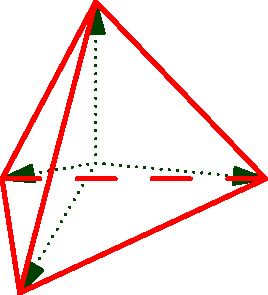
\includegraphics{./Eisogo_2.pdf}
 % Eisogo_2.pdf: 0x0 pixel, 0dpi, 0.00x0.00 cm, bb=
 \caption{Tétraèdre isogonal}
 \label{fig:Eisogo_2}
\end{figure}
Dans cette partie, $B=\{u_1,u_2,u_3,u_4\}$ est un ensemble $-\frac{1}{3}$-isogonal dans un espace $E$ euclidien de dimension $3$.
\begin{enumerate}
\item Montrer que trois vecteurs de $B$ deux {\`a} deux distincts forment une base de $E$. Quelles sont les composantes du vecteur $u_4$ dans la base $\{u_1,u_2,u_3\}$ ?
\item Montrer que pour tout $x$ de $E$, il existe un unique quadruplet $(m_1,m_2,m_3,m_4)\in \R^4$ tel que
\[ \sum_{i=1}^4 m_i=1 \quad \text{et} \quad x=\sum_{i=1}^4m_iu_i\]
On dira que $m_1$, $m_2$, $m_3$, $m_4$ sont les \emph{coordonnées barycentriques} de $x$ dans $B$.
\item On d{\'e}signe par $T$ l'ensemble des vecteurs dont les coordonnées barycentriques dans $B$ sont positives ou nulles. Soit $f$ un automorphisme orthogonal de $E$. On se propose de d{\'e}montrer 
\begin{displaymath}
 f(B)=B \Leftrightarrow f(T)=T
\end{displaymath}
\begin{enumerate}
\item Montrer que $f(B)=B \Rightarrow f(T)=T $.
\item On suppose $f(T)=T$, soit $u\in B$ et $v=f(u)$.\newline
Pourquoi $v$ est-il {\'e}l{\'e}ment de $T$?\newline
On note $(m_1,m_2,m_3,m_4)$ la famille des coordonnées barycentriques de $v$. Montrer que
\[||v||^2=\sum_{i=1}^4m_i^2-\frac{2}{3}\sum_{1\leq i < j \leq  4}m_im_j\]
Calculer
\[\left( \sum_{i=1}^4m_i \right)^2-||v||^2\]
et montrer que
\[\sum_{1\leq i < j \leq 4}m_im_j=0\]
En d{\'e}duire qu'il existe un entier $i$ entre 1 et 4 tel que $m_i=1$ et que les autres $m_j$ soient nuls. Conclure.
\end{enumerate}
\item On d{\'e}signe par $G$ le groupe des bijections de $B$ sur $B$. Soit $\sigma$ un {\'e}l{\'e}ment de $G$.
\begin{enumerate}
\item Montrer qu'il existe un unique endomorphisme $\overline{\sigma}$ du $\R$-espace vectoriel $E$ tel que $\overline{\sigma}(u_i)=\sigma(u_i)$ pour $i=1,2,3$.
\item Montrer que $\overline{\sigma}$ est un automorphisme orthogonal de $E$.
\item Montrer que  $\overline{\sigma}(u_4)=\sigma(u_4)$.
\item Montrer que l'ensemble $\mathcal{G}$ des automorphismes orthogonaux $g$ de $E$ tels que $g(T)=T$ est un sous-groupe du groupe orthogonal de $E$.\newline
Montrer que l'application qui {\`a} $g\in \mathcal{G}$ associe la restriction de $g$ {\`a} $B$ est un isomorphisme de groupe de $\mathcal{G}$ vers $G$. Quel est le cardinal de $\mathcal{G}$?
\item Pour tout couple $(i,j)$ d'entiers distincts entre 1 et 4, on d{\'e}signe par $H_{i,j}$ le plan vectoriel orthogonal {\`a} $u_i-u_j$ et par $\tau_{i,j}$ la r{\'e}flexion par rapport {\`a} $H_{i,j}$. Utiliser l'isomorphisme entre $\mathcal{G}$ et $G$ pour montrer que tout
{\'e}l{\'e}ment de $\mathcal{G}$ est une composition d'un nombre fini de $\tau_{i,j}$.
\end{enumerate}
\end{enumerate}
%
\newpage%
\section*{Problème 17}%
\addcontentsline{toc}{section}{Pb 17 : Un problème d'analyse "à la Cauchy" sur un ensemble de réels défini à partir d'une fonction.}%
\fancyhead[LO,RE]{Énoncés - Pb 17 : Un problème d'analyse "à la Cauchy" sur un ensemble de réels défini à partir d'une fonction.}%
%<dscrpt>Un problème d'analyse "à la Cauchy" sur un ensemble de réels défini à partir d'une fonction.</dscrpt>
Soit $g$ une application continue dans un segment r{\'e}el $\left[a,b\right]$ et {\`a} valeurs r{\'e}elles. On se propose d'{\'e}tudier l'ensemble
\[
E= \left\lbrace  x\in \left] a,b\right[ \text{ tq }\exists \xi \in \left]
x,b\right] \text{ tq }g(x)<g(\xi )\right\rbrace  \text{.}
\]

\subsection*{Partie I}

\begin{enumerate}
\item  D{\'e}terminer $E$ dans les cas suivants.

\begin{enumerate}
\item La fonction $g$ est strictement croissante,

\item  $a=-1$, $b=1$ et $g(t)=1-t^{2}$.

\item  $a=0$, $b=2\pi $ et $g(t)=\sin t$.

\item  $a=-1$, $b=1$ et $g(t)=-t^{4}+t^{2}$.
\end{enumerate}

\item  Dessiner le graphe d'une fonction $g$ telle que $E$ contienne un maximum local.

\item  En g{\'e}n{\'e}ral, une fonction strictement d{\'e}croissante dans $\left] a,b \right] $ l'est-elle encore dans $\left[ a,b \right] $? Et si on suppose
de plus la continuit{\'e} en $a$ ?

\item
\begin{enumerate}
\item  Montrer que $E$ est vide si et seulement si $g$ est d{\'e}croissante dans $\left[ a,b \right]$.

\item Soit $M=\sup_{\left[ a,b \right]}(g)$, montrer que $E=]a,b[$ entra\^{\i }ne $M\in \{ g(a),g(b)\}$. Illustrer les deux possibilit{\'e}s en dessinant un graphe. La r{\'e}ciproque est-elle vraie?
\end{enumerate}
\end{enumerate}

\subsection*{Partie II}

La fonction $\psi $ est d{\'e}finie dans $\left[ a,b \right]$ par
\[
\psi (x)=\sup_{[x,b]}g.
\]

\begin{enumerate}
\item  Montrer que $\psi $ est monotone et continue, pr{\'e}ciser son sens de variation.

\item
\begin{enumerate}
\item  Caract{\'e}riser les {\'e}l{\'e}ments de $E$ {\`a} l'aide des fonctions $\psi $ et $g$.
\item  Montrer que si $x\in E$, il existe $\alpha >0$ tel que $]x-\alpha ,x+\alpha[ \subset E$.
\end{enumerate}

\item Si $x\in E$, on note
\[
s(x)=\inf \left\{ \xi \in \left] x,b \right] \text{ tq } g(x) < g(\xi ) \right\}
\]

\begin{enumerate}
\item Montrer que $s(x)>x$ entraine $s(x)\in [x,b[$ et $g(y)\leq g(x)$ pour tout $y$ dans $[x,s(x)[$.

\item Montrer que $g(s(x))=g(x)$ et que $[x,s(x)[ \subset E$.
\end{enumerate}
\end{enumerate}
%
\newpage%
\section*{Problème 18}%
\addcontentsline{toc}{section}{Pb 18 : Nombres complexes et fonctions usuelles : autour de la formule de Machin.}%
\fancyhead[LO,RE]{Énoncés - Pb 18 : Nombres complexes et fonctions usuelles : autour de la formule de Machin.}%
%<dscrpt>Nombres complexes et fonctions usuelles : autour de la formule de Machin.</dscrpt>
L'objet de ce problème est de présenter la formule de Machin \footnote{John Machin (1680 - 1752). Grâce à cette formule, en 1706, Machin est le premier mathématicien à calculer 100 décimales de $\pi$.} et quelques résultats autour.
\[\frac{\pi}{4}=4\arctan\frac{1}{5}-\arctan\frac{1}{239}\]
On obtiendra diverses formules faisant intervenir des $\arctan$ d'inverses de nombres. En particulier, une formule du type Machin est de la forme
\begin{displaymath}
m\arctan\frac{1}{x}+\arctan\frac{1}{y}\equiv\frac{\pi}{4} \mod \pi \text{ avec } m, x, y \text{ entiers}
\end{displaymath}

\subsection*{Partie I. Introduction. Exemples}
Pour tout entier naturel non nul $m$, on appelle $\mathcal{C}_m$ l'ensemble des couples de réels non nuls $(x,y)$ tels que
\[m\arctan\frac{1}{x}+\arctan\frac{1}{y}\equiv\frac{\pi}{4}\;(\pi)\]
\begin{enumerate}
\item Pour $x$ réel non nul, on pose $\alpha=\arctan\frac{1}{x}$. Exprimer $x+i$ à l'aide de $\alpha$ et de l'exponentielle complexe. Donner un argument de $x+i$.
\item Montrer que
\[(x,y)\in \mathcal{C}_m\Leftrightarrow (x+i)^m(y+i)e^{-i\frac{\pi}{4}}\in \R\]
\item Montrer que
\[\frac{\pi}{4}=2\arctan\frac{1}{2}-\arctan\frac{1}{7}\]
\item Formule de Dodgson\footnote{plus connu pour son oeuvre littéraire sous le pseudonyme Lewis Carrol}\newline
Soit $p$, $q$, $r$ trois réels positifs tels que $1+p^2=qr$. Montrer que
\[\arctan\frac{1}{p}=\arctan\frac{1}{p+r}+\arctan\frac{1}{p+q}\]
\end{enumerate}

\subsection*{Partie II. {\'E}tude d'une famille de polynômes}
Pour $x$ réel et $m$ entier positif, on note respectivement $A_m(x)$ la partie réelle et $B_m(x)$ la partie imaginaire de de $(x+i)^m$. On définit également $F_m$ par :
\[F_m(x)=\frac{A_m(x)+B_m(x)}{A_m(x)-B_m(x)}\]
\begin{enumerate}
\item Calculer les polynômes $A_k(x)$ et $B_k(x)$ pour $k\in\{1,2,3,4\}$. Présenter les résultats dans un tableau.
\item Montrer les relations suivantes liant les polynômes et leurs dérivées
\begin{center}
\renewcommand{\arraystretch}{1.8}
\begin{tabular}{ll}
$A_{m+1}(x) = xA_m(x)-B_m(x)$   & $A_{m}(-x) = (-1)^m A_m(x)$   \\
$B_{m+1}(x) = A_m(x) +x B_m(x)$ & $B_{m}(-x) = -(-1)^m B_m(x)$  \\
$A'_{m}(x) = m A_{m-1}(x)$      & $B'_{m}(x) = m B_{m-1}(x)$
\end{tabular}
\end{center}
Montrer aussi que
\begin{center}
\renewcommand{\arraystretch}{1.8}
\begin{tabular}{c|c}
si $m$ pair & si $m$ impair\\ \hline
$A_{m}(x) = (-1)^{\frac{m}{2}}x^m A_{m}(-\frac{1}{x})$ & $A_{m}(x) = (-1)^{\frac{m-1}{2}}x^m B_{m}(-\frac{1}{x})$\\ \hline 
$B_{m}(x) = (-1)^{\frac{m}{2}}x^m B_{m}(-\frac{1}{x})$ & $B_{m}(x) = -(-1)^{\frac{m-1}{2}}x^m A_{m}(-\frac{1}{x})$
\end{tabular}
\end{center}

\item Pour un entier $m$ fixé, déterminer les solutions de $A_m(x)=B_m(x)$. Quelle est la plus grande de ces solutions ?
\item Montrer que la fonction $F_m$ est décroissante dans chaque intervalle de son domaine de définition. Quelle est la limite de $F_m$ en $+\infty$ et en $-\infty$ ?
\end{enumerate}

\subsection*{Partie III. Les formules du type Machin}
On cherche \emph{toutes} les formules du type Machin pour $m$ entre 1 et 4.
\begin{enumerate}
\item Montrer que pour tout $(x,y)$ de $\R^2$,
\begin{displaymath}
(x,y)\in \mathcal{C}_m \Leftrightarrow \left( A_m(x) \neq B_m(x) \text{ et } y=F_m(x)\right) 
\end{displaymath}

\item Des calculs numériques conduisent aux tableaux suivants:
\begin{center}
% use packages: array
\renewcommand{\arraystretch}{1.5}
\hspace{1cm}
\begin{tabular}{c|c}
 $m$ & $\cotan\left( \frac{\pi}{4m}\right) $ \\ \hline 
1 &  1 \\ \hline
2 &  2.414\\ \hline
3 & 3.732 \\ \hline
4 & 5.027
\end{tabular}
\hfill
\begin{tabular}{c|c|c|c|c}
$x$ & $F_1(x)$ & $F_2(x)$ & $F_3(x)$ & $F_4(x)$ \\ \hline
1   &          & -1.      & 0.       & 1.       \\ \hline
2   & 3.       & -7.      & -1.444   & -.5484   \\ \hline
3   & 2.       & 7.       & -5.500   & -1.824   \\ \hline
4   & 1.667    & 3.286    & 19.80    & -5.076   \\ \hline
5   & 1.500    & 2.429    & 5.111    & -239.0   \\ \hline
6   & 1.400    & 2.043    & 3.352    & 7.971    \\ \hline
7   & 1.333    & 1.824    & 2.659    & 4.518    \\ \hline
8   & 1.286    & 1.681    & 2.286    & 3.376    \\ \hline
9   & 1.250    & 1.581    & 2.052    & 2.802    \\ \hline
10  & 1.222    & 1.506    & 1.891    & 2.455    \\ \hline
11  & 1.200    & 1.449    & 1.774    & 2.222    \\ \hline
12  & 1.182    & 1.403    & 1.684    & 2.055    \\ \hline
13  & 1.167    & 1.366    & 1.613    & 1.929
\end{tabular} 
\hspace*{1.5cm}
\end{center}
{\`A} partir de ces tableaux, former (en justifiant soigneusement) toutes les formules du type Machin pour $m$ entier entre $1$ et $4$.
\end{enumerate}

\subsection*{Partie IV. Algorithme de Lehmer.}
Soit $z_0$ un nombre complexe dont la partie imaginaire est strictement positive. On définit des complexes $z_1$, $z_2$, $\cdots$ par récurrence en posant
\begin{displaymath}
 z_{k+1}=z_k(-\lfloor\frac{\Re (z_k)}{\Im (z_k)}\rfloor + i) \text{ lorsque } \Im (z_k) \neq 0
\end{displaymath}
(la notation $\lfloor . \rfloor$ désignant la fonction partie entière). L'algorithme s'arrête quand un nombre réel est obtenu. On pourra noter
\[n_k = \lfloor \frac{\Re (z_k)}{\Im (z_k)}\rfloor \]
\begin{enumerate}
\item Faire les calculs dans le cas particulier $z_0=17+7i$.
\item Montrer que la suite formée par les parties imaginaires des $z_k$ est strictement décroissante et à valeurs positives.
\item On suppose que $z_0=a+ib$ avec $a$ et $b$ entiers strictement positifs.
\begin{enumerate}
\item Montrer qu'il existe un $k$ tel que $z_k$ est réel.
\item En déduire que
\[\arctan(\frac{b}{a}) \equiv \arctan(\frac{1}{n_0})+\arctan(\frac{1}{n_1}) + \cdots + \arctan(\frac{1}{n_{k-1}}) \; (\pi)\]
en convenant que, si un des $n_i$ est nul, on remplace $\arctan(\frac{1}{n_i})$ par $\frac{\pi}{2}$.
\end{enumerate}
\end{enumerate}
%
\newpage%
\section*{Problème 19}%
\addcontentsline{toc}{section}{Pb 19 : Chemins et nombres de Catalan.}%
\fancyhead[LO,RE]{Énoncés - Pb 19 : Chemins et nombres de Catalan.}%
%<dscrpt>Chemins et nombres de Catalan.</dscrpt>
Pour tout le problème, $a$ et $b$ désignent des entiers naturels tels que $a < b$. 
Dans un plan muni d'un repère orthonormé $(O,(\overrightarrow i , \overrightarrow j))$ dont les fonctions coordonnées sont notées $x$ et $y$, on fixe certaines définitions et notations.
\begin{itemize}
 \item Un point $M$ est \emph{sur la diagonale} si et seulement si $x(M) = y(M)$.
 \item Un point $M$ est \emph{au dessous de la diagonale} si et seulement si $y(M) \leq x(M)$.
 \item Un point $M$ est \emph{strictement au dessous de la diagonale} si et seulement si $y(M) < x(M)$.
 \item On appelle \emph{chemin} une famille de points à coordonnées entières 
\begin{displaymath}
 (M_0,M_1,\cdots M_p) \text{ tq } \forall k\in \llbracket 0, p-1 \rrbracket,\; 
\overrightarrow{M_kM_{k+1}}\in \{\overrightarrow i , \overrightarrow j\}
\end{displaymath}
On dit que les $M_k$ sont les points du chemin, que ce chemin est de longueur $p$ et qu'il va de $M_0$ à $M_p$ (extrémités du chemin).
 \item On désigne par $\mathcal{P}_{a,b}$ l'ensemble des chemins allant du point de coordonnées $(a,a)$ au point de coordonnées  $(b,b)$.
 \item On désigne par $\mathcal{C}_{a,b}$ l'ensemble des chemins appartenant à $\mathcal{P}_{a,b}$ et dont tous les points sont au dessous de la diagonale.
 \item On désigne par $\mathcal{C}'_{a,b}$ l'ensemble des chemins appartenant à $\mathcal{P}_{a,b}$ et dont tous les points (sauf les extrémités) sont strictement au dessous de la diagonale.
 \item Si $\Gamma = (M_0,M_1,\cdots M_p)\in \mathcal{C}_{a,b}$, on note $m(\Gamma)$ le plus petit des $x(M_k)>0$ tels que $M_k$ soit sur la diagonale.
 \item Pour $n\in \N^*$, on note $c_n$ le nombre d'éléments de $\mathcal{C}_{0,n}$. On convient que $c_0=1$.
\end{itemize}
La figure \ref{fig: Enbcat_1} montre le dessin obtenu en reliant les points d'un chemin $\Gamma \in \mathcal{C}_{0,5}$ par des segments. Que vaut $m(\Gamma)$ sur cet exemple?
\begin{figure}[h!t]
 \centering
 \includegraphics{./Enbcat_1.pdf}
 % Enbcat_1.pdf: 0x0 pixel, 0dpi, 0.00x0.00 cm, bb=
 \caption{Chemin appartenant à $\mathcal{C}_{0,5}$}
 \label{fig: Enbcat_1}
\end{figure}
  
\begin{enumerate}
 \item Soit $n\in \N^*$.
\begin{enumerate} 
 \item Quelle est la longueur d'un chemin appartenant à $\mathcal{P}_{0,n}$ ?
 \item Calculer le nombre d'éléments de $\mathcal{P}_{0,n}$ en le mettant en bijection avec un ensemble usuel.
\end{enumerate}
\item 
\begin{enumerate}
 \item Préciser $c_1$ et $c_2$.
 \item Exprimer le nombre d'éléments de $\mathcal{C}_{a,b}$ à l'aide d'un $c_k$ pour un entier $k$ à préciser.
 \item Soit $m\in \N^*$, exprimer le nombre d'éléments de $\mathcal{C}'_{0,m}$ à l'aide d'un $c_k$ pour un entier $k$ à préciser.
 \item Montrer que
\begin{displaymath}
 \forall n\in \N^*,\; c_n =\sum_{m=1}^{n}c_{m-1}c_{n-m} 
\end{displaymath}
En déduire que
\begin{displaymath}
 \forall n\in \N,\; c_{n+1} =\sum_{k=0}^{n}c_{k}c_{n-k} 
\end{displaymath}
\end{enumerate}
\item Les nombres $c_n$ sont appelés les \emph{nombres de Catalan}, ils interviennent dans diverses questions de dénombrement. On se propose de démontrer par récurrence que
\begin{displaymath}
 c_n = \frac{\binom{2n}{n}}{n+1}
\end{displaymath}
Dans cette question, $n$ est un naturel quelconque, notons
\begin{displaymath}
 a_n= \frac{\binom{2n}{n}}{n+1}
,\hspace{0.5cm} S_{n} =\sum_{k=0}^{n}a_{k}a_{n-k}
,\hspace{0.5cm} T_{n} =\sum_{k=0}^{n}ka_{k}a_{n-k}
\end{displaymath}
en convenant que $a_0=1$. 
\begin{enumerate}
 \item Montrer $2T_n = n S_n$. En déduire $T_{n+1}+S_{n+1} = \frac{n+3}{2}S_{n+1}$.
 \item Montrer $(k+2)a_{k+1} = 2(2k+1)a_k$. En déduire $ T_{n+1}+S_{n+1} = a_{n+1} + 4T_n +2S_n $.
 \item Montrer que $S_n=a_{n+1}$ entraine $S_{n+1}=a_{n+2}$ et conclure.
\end{enumerate}

\end{enumerate}
%
\newpage%
\section*{Problème 20}%
\addcontentsline{toc}{section}{Pb 20 : Exemples de produits infinis.}%
\fancyhead[LO,RE]{Énoncés - Pb 20 : Exemples de produits infinis.}%
%<dscrpt>Exemples de produits infinis.</dscrpt>
Soit $(u_n)_{n\in \N^*}$ une suite de réels non nuls, on lui associe la suite $(p_n)_{n\in \N^*}$ définie par :
\[p_n=u_1 u_2 \cdots u_n\]
On dira que le produit infini $\prod_{n\geq 1}u_n$ converge si et seulement la suite $(p_n)_{n\in \N^*}$ converge vers un nombre \emph{non nul}. Cette limite sera notée  $\prod_{n\geq 1}u_n$. Si la suite $(p_n)$ ne converge pas, on dira que le produit diverge.
\subsection*{I. Exemples.}
\begin{enumerate}
  \item Soit $u_k = 1 + \frac{1}{k}$.\newline
  Simplifiez $p_n$. Le produit $\prod_{n\geq 1}(1+\frac{1}{n})$ est-il divergent ou convergent ?
  
  \item Soit $u_k=\cos \frac{a}{2^k}$ avec  $a \not \equiv 0 \mod \pi$.\newline
Pour tout $n\in \N^*$, calculer $p_n\sin\frac{a}{2^n}$. En déduire que le produit infini converge et préciser 
\[
 \prod_{n\geq 1}\cos \frac{a}{2^n} .
\]

  \item Soit $u_k = 1 - \frac{1}{k^2}$ pour $k\geq 2$. Montrer que le produit infini converge et calculer 
\[
 \prod_{n\geq 2}(1 - \frac{1}{n^2}).
\]

 \item Soit $a \in ]0,1[$ et $u_k = 1 + a^{(2^k)}$. Calculer $(1-a^2)p_n$. En déduire la convergence et la valeur du produit infini.  
\end{enumerate}

\subsection*{II. Conditions.}
\begin{enumerate}
 \item Montrer que si le produit infini $\prod_{n\geq 1}u_n$ converge alors la suite $(u_n)_{n\in \N^*}$ converge vers 1.
 
 \item On suppose $u_n >0$ à partir d'un certain rang $n_0$.\newline
 Montrer que la convergence du produit infini $\prod_{n\geq 1}u_n$ est équivalent à la convergence de la série $(\sum \ln(u_n))_{n \geq n_0}$. Dans ce cas, comment sont reliés la valeur du produit infini et la somme de la série?
 
 \item Montrer que, sous l'une des hypothèses suivantes
 \begin{itemize}
   \item à partir d'un certain rang $n_0$, $u_n = 1 - v_n$ avec $0 < v_n < 1$,
   \item à partir d'un certain rang $n_0$, $u_n = 1 + v_n$ avec $0 < v_n$,
 \end{itemize}
le produit infini $\prod_{n\geq 1} u_n$ converge si et seulement si la série  $ \left( \sum v_n \right)_{n\geq n_0}$ converge.
\end{enumerate}

\subsection*{III. Un expression de $\sin$ comme produit infini.}
Dans cette partie, $x\in ] -1 , 1[$.
\begin{enumerate}
 \item 
 \begin{enumerate}
  \item Montrer la convergence de la série $(\sum \frac{2x}{x^2 - n^2})_{n\geq 1}$.
  \item Montrer la convergence du produit infini $\prod_{n\geq 1}(1-\frac{x^2}{n^2})$.
 \end{enumerate}

 \item \'Etudes locales.
 \begin{enumerate}
  \item Former un développement asymptotique en $0$ avec un reste en $o(t)$ de 
 \[
  t \mapsto \pi \cot (\pi t).
 \]
  \item Montrer que l'on peut prolonger par continuité la fonction définie par : 
  \[
 \forall t \in ]-1,+1[\setminus\left\lbrace 0\right\rbrace,\;  t \mapsto \ln\left( \frac{\sin \pi t}{\pi t}\right).
  \]
On note $f$ la fonction ainsi prolongée.
  \item Montrer que $f$ est $\mathcal{C}^1$ dans $]-1,+1[$ et préciser $f'$.
 \end{enumerate}

   \item On admet la relation suivante
\[
 \forall x \in ]-1,1[,\; f'(x) = \sum_{n\geq 1} \frac{2x}{x^2 - n^2}. 
\]
\begin{enumerate}
 \item Montrer que 
 \[
  \forall t\in ]0,1[, \forall n\in \N\setminus\left\lbrace 0,1\right\rbrace,  \; \frac{t}{n^2 - t^2} \leq \frac{1}{n^2 - 1}
 \]
  \item Montrer que
\[
\forall N\in \N^*, \, \forall x \in ]-1, +1[\;
 \left|\ln\left( \frac{\sin(\pi x)}{\pi x}\right) - \sum_{n=1}^{N}\int_{0}^{x}\frac{2t}{t^2 - n^2}\, dt\right|
 \leq |x| \sum_{n = N+1}^{+\infty}\frac{2}{n^2 -1}.
\]

 \item En déduire 
\[
 \forall x\in ]-1 , +1 [, \; \sin(\pi x) = \pi x \prod_{n \geq 1}\left( 1 - \frac{x^2}{n^2}\right) .
\]

\end{enumerate}

\end{enumerate}

%
\newpage%
\section*{Problème 21}%
\addcontentsline{toc}{section}{Pb 21 : Introduction aux polynômes orthogonaux}%
\fancyhead[LO,RE]{Énoncés - Pb 21 : Introduction aux polynômes orthogonaux}%
%<dscrpt>Introduction aux polynômes orthogonaux</dscrpt>
On note\footnote{d'après \textit{Fractions et Polynômes} éd Ellipses} $E$ le $\R$ espace vectoriel $\R[X]$ des polynômes à coefficients réels et $E_n$ le sous-espace formé par les polynômes dont le degré est inférieur ou égal à $n$. On identifiera dans ce texte un polynôme avec la fonction polynomiale qui lui est associée. Le $\R$ espace vectoriel $E$ est muni d'un produit scalaire vérifiant la propriété suivante :
\begin{displaymath}
 \forall (P,Q)\in E^2,\quad (XP/Q)=(P/XQ)
\end{displaymath}
Il est important de bien comprendre que $(P/Q)$ désigne le nombre réel produit scalaire des éléments $P$ et $Q$ de $E$.\\
Notons $1_E$ le polynôme constant 1 et $c_i=(X^i/1_E)$ pour tout entier naturel $i$.\\
On dira que $(P_n)_{n\in \N}$ est une \emph{suite de polynômes orthogonaux} lorsque
\begin{displaymath}
  \begin{aligned}
    \forall n\in \N &, \deg (P_n)=n \\
    \forall (i,j)\in \N^2 &, i<j \Rightarrow (X^i / P_j)=0
  \end{aligned}
\end{displaymath}

On définit une suite de fonctions polynomiales $(D_n)_{n\in \N}$ et une suite de nombres réels $(\Delta_n)_{n\in \N}$ par $\Delta_0=1$, $D_0=1_E$ et les formules suivantes (déterminants) qui sont valables pour tout entier non nul $n$ 
\begin{displaymath}
 \Delta_n = \left \vert
\begin{array}{ccccc}
 c_0 & c_1 & \cdots & c_{n-1} & c_n \\
 c_1 & c_2 & \cdots & c_{n} & c_{n+1} \\
 \vdots & \vdots & \ddots & \vdots & \vdots \\
 c_{n-1} & c_n & \cdots & c_{2n-2} & c_{2n-1} \\
c_n & c_{n+1} & \cdots & c_{2n-1} & c_{2n}
\end{array}
\right \vert
\end{displaymath}
\begin{displaymath}
\forall x\in \R:  D_n(x) = \left \vert
\begin{array}{ccccc}
 c_0 & c_1 & \cdots & c_{n-1} & c_n \\
 c_1 & c_2 & \cdots & c_{n} & c_{n+1} \\
 \vdots & \vdots & \ddots & \vdots & \vdots \\
 c_{n-1} & c_n & \cdots & c_{2n-2} & c_{2n-1} \\
1 & x & \cdots & x^{n-1} & x^n
\end{array}
\right \vert
\end{displaymath}

\subsection*{Partie I}
\begin{enumerate}
 \item 
  \begin{enumerate}
    \item Cas particulier. Montrer que l'on définit un produit scalaire vérifiant les conditions de l'énoncé en posant
\begin{displaymath}
 (P/Q)=\int_{-1}^{1}P(x)Q(x)dx
\end{displaymath}
pour tout couple $(P,Q)$ de polynômes.
    \item Calculer $c_n$ pour tout entier $n$ ainsi que $\Delta_1$, $\Delta_2$, $D_1$, $D_2$, $D_3$.
\end{enumerate}
 
\item Montrer que $(D_n)_{n\in \N}$ est une suite de polynômes orthogonaux. Quels sont les coefficients dominants ?

\item \begin{enumerate}
 \item Soit $(P_n)_{n\in \N}$ une suite de polynômes orthogonaux et $Q$ un polynôme de degré strictement inférieur à $n$, montrer que
 \begin{displaymath}
   (P_n / Q)=0
 \end{displaymath}
 \item Soit $(P_n)_{n\in \N}$ une suite de polynômes orthogonaux et $(\lambda_n)_{n\in \N}$ une suite de nombres réels non nuls. Montrer que $(\lambda_n P_n)_{n\in \N}$ est une suite de polynômes orthogonaux.
 \item Soit $(P_n)_{n\in \N}$ et $(Q_n)_{n\in \N}$ deux suites de polynômes orthogonaux, montrer qu'il existe une suite $(\lambda_n)_{n\in \N}$ de nombres réels non nuls tels que $Q_n=\lambda_n P_n$ pour tous les entiers $n$.
\end{enumerate}

Dans toute la suite, on notera $(Q_n)_{n\in \N}$ l'\emph{unique} suite de polynômes orthogonaux telle que le coefficient dominant de chaque $Q_n$ soit égal à 1.

\item \begin{enumerate}
 \item Exprimer $D_n$ en fonction de $\Delta_{n-1}$ et de $Q_n$.
 \item Montrer que, pour tout entier $n$ :
\begin{displaymath}
 (Q_n / X^n) = \Vert Q_n \Vert ^2
\end{displaymath}
Exprimer cette quantité en fonction de $\Delta_{n-1}$ et $\Delta_n$
\end{enumerate}

\item Relation de récurrence.
\begin{enumerate}
 \item Soit $(P_n)_{n\in \N}$ une suite de polynômes orthogonaux. Montrer qu'il exsite des suites $(\alpha_n)_{n\in \N}$, $(\beta_n)_{n\in \N}$, $(\gamma_n)_{n\in \N}$ telles que, pour tous les entiers $n\geq1$:
\begin{displaymath}
 XP_n = \alpha_n P_{n-1}+ \beta_n P_n +\gamma_n P_{n+1}
\end{displaymath}
\item Montrer qu'il existe des suites $(a_n)_{n\in \N}$ et $(b_n)_{n\in \N}$ telles que 
\begin{displaymath}
 \forall n\geq 2 : \quad Q_n = (a_n + X)Q_{n-1}+b_nQ_{n-2}
\end{displaymath}


\end{enumerate}

\end{enumerate}

\subsection*{Partie II}
Dans cette partie, on se propose de calculer explicitement les coefficients de la relation de récurrence vérifiée par les polynômes orthogonaux qui prennent en 1 la valeur 1 (polynômes de Legendre) pour le cas particulier de la question I.1.\newline
On garde les notations de la partie I et on désigne par $(L_n)_{n\in \N}$ l'unique suite de polynômes orthogonaux vérifiant $L_n(1)=1$ pour tout entier $n$. 
\begin{enumerate}
 \item Comment s'expriment les $L_n$ en fonction des $Q_n$ ?
 \item Montrer que pour tout entier $n$ : 
\begin{displaymath}
L_n(-x)= (-1)^n L_n(x)
\end{displaymath}
\item Montrer que $\beta_n=0$ pour tout entier $n$. (on pourra prendre la valeur en $1$ et en $-1$)
\item Soit $\lambda_n$ le coefficient dominant de $L_n$, exprimer $\alpha_n$ en fonction de $\lambda_{n-1}$, $\lambda_{n}$, $\Vert L_{n-1}\Vert ^2$, $\Vert L_{n}\Vert ^2$. Exprimer $\gamma_n$ en fonction de $\lambda_{n+1}$, $\lambda_{n}$.

\item En considérant $(L_n^\prime / L_{n-1})$, montrer que
\begin{displaymath}
 n\frac{\lambda_n}{\lambda_{n-1}} \Vert L_{n-1} \Vert^2 = 2
\end{displaymath}

\item Montrer que
\begin{displaymath}
 \Vert L_n \Vert ^2 = \frac{1}{2n+1}
\end{displaymath}
Préciser la relation de récurrence vérifiée par la suite $(Q_n)_{n\in \N}$.
\end{enumerate}
%
\newpage%
\section*{Problème 22}%
\addcontentsline{toc}{section}{Pb 22 : Rotations, angles d'Euler, quaternions}%
\fancyhead[LO,RE]{Énoncés - Pb 22 : Rotations, angles d'Euler, quaternions}%
%<dscrpt>Rotations, angles d'Euler, quaternions</dscrpt>
Dans la première partie, on introduit des \emph{angles d'Euler} pour repérer les rotations d'un espace vectoriel euclidien orienté de dimension 3.\newline 
Dans la suite on introduit les \emph{quaternions de Hamilton} comme des matrices $2\times2$ à coefficients complexes et diverses structures sur cet espace. On définit en particulier un $\R$-espace vectoriel euclidien de dimension $3$ formé de quaternions dits \emph{purs}. Bien que, de nature matricielle par définition, les quaternions purs seront regardés le plus souvent comme des vecteurs. On retrouve à la fin les angles d'Euler en termes de quaternions.

\subsection*{Partie I - Angles d'Euler}
\begin{figure}
   \centering
   %\includegraphics[scale=0.5]{Equateuler.pdf}
   \input{Equateuler_1.pdf_t}
   \caption{Angles d'Euler}
   %\label{}
\end{figure}
 Soit $(\overrightarrow{i},\overrightarrow{j},\overrightarrow{k})$ et $(\overrightarrow{i_1},\overrightarrow{j_1},\overrightarrow{k_1})$ deux bases orthonormées directes. On suppose que $(\overrightarrow{k},\overrightarrow{k_1})$ est libre. Il existe alors une unique rotation $r$ telle que
 \[r(\overrightarrow{i})=\overrightarrow{i_1},
 r(\overrightarrow{j})=\overrightarrow{j_1},
 r(\overrightarrow{k})=\overrightarrow{k_1}\]
 On se propose de définir les trois \emph{angles d'Euler} $\theta, \varphi, \psi$ qui permettent de repérer $(\overrightarrow{i_1},\overrightarrow{j_1},\overrightarrow{k_1})$ et de décomposer $r$ en trois rotations d'angles $\theta, \varphi, \psi$ autour d'axes orientés s'exprimant très simplement avec $(\overrightarrow{i},\overrightarrow{j},\overrightarrow{k})$.
 
 Soit $\theta$ l'écart angulaire entre $\overrightarrow{k}$ et $\overrightarrow{k_1}$.
 Il existe un unique vecteur unitaire $\overrightarrow{u}$ orthogonal à $\overrightarrow{k}$ et $\overrightarrow{k_1}$ tel que $\overrightarrow{k_1}=r_{\overrightarrow{u},\theta}(\overrightarrow{k})$. On notera 
\begin{displaymath}
r_1=r_{\overrightarrow{u},\theta} 
\end{displaymath}
 Soit $\varphi$ l'unique réel dans $[0,2\pi[$ tel que $\overrightarrow{u} = r_{\overrightarrow{k},\varphi}(\overrightarrow{i})$. On notera
 \[r_2=r_{\overrightarrow{k},\varphi}\]
 Soit $\psi$ l'unique réel dans $[0,2\pi[$ tel que $\overrightarrow{i_1} = r_{\overrightarrow{k_1},\psi}(\overrightarrow{u})$. On notera
 \[r_3=r_{\overrightarrow{k_1},\psi}\]
 \begin{enumerate}
\item Calculer $r_3\circ r_1 \circ r_2 (\overrightarrow{i})$ et $r_3\circ r_1 \circ r_2 (\overrightarrow{k})$. En déduire que $r_3\circ r_1 \circ r_2=r$.
\item Soit $\overrightarrow{w}$ un vecteur non nul, $\alpha$ un réel quelconque et $f$ une rotation. Montrer que
\[f\circ r_{\overrightarrow{w},\alpha} \circ f^{-1}=r_{f(\overrightarrow{w}),\alpha}\]

\item On adopte les notations suivantes:
\begin{displaymath}
r_\varphi=r_2=r_{\overrightarrow{k},\varphi},\hspace{0.5cm} r_\psi=r_{\overrightarrow{k},\psi},\hspace{0.5cm} R_\theta=r_{\overrightarrow{i},\theta} 
\end{displaymath}
Que valent $r_\varphi(\overrightarrow{i})$ et $r_1(\overrightarrow{k})$ ? Exprimer $r_1$ à l'aide de $r_\varphi$ et $R_\theta$. En déduire
\[r=r_\varphi \circ R_\theta \circ r_\psi\] 
{\'E}crire sous la forme d'un produit, la matrice de $r$ dans la base $(\overrightarrow{i},\overrightarrow{j},\overrightarrow{k})$. 
\end{enumerate} 

\subsection*{Partie II - Quaternions.}
On appelle \emph{quaternion} toute matrice complexe
\[q=\begin{pmatrix}
 a & -\overline{b}  \\ 
 b & \overline{a}
\end{pmatrix} \quad \text{ avec } (a,b)\in\C ^2\]
On note $\mathbb{H}$ l'ensemble des quaternions et on adopte les conventions suivantes :
\begin{eqnarray*}
\overline{q} &=& \begin{pmatrix}
 \overline{a} & \overline{b}  \\ 
 -b & a
\end{pmatrix}\\
N(q) &=& \det(q)=|a|^2+|b|^2
\end{eqnarray*}
Un quaternion $q$ est dit \emph{vectoriel} ou \emph{pur} si et seulement si $\overline{q}=-q$.\newline
On note $E$ l'ensemble des quaternions purs, ils seront écrits généralement avec une flèche. On pose en particulier
\[1_{\mathbb{H}}=\begin{pmatrix}
 1 & 0  \\ 
 0 & 1
\end{pmatrix},\hspace{0.3cm}
\overrightarrow{i}=\begin{pmatrix}
 0 & i  \\ 
 i & 0
\end{pmatrix},\hspace{0.3cm}
\overrightarrow{j}=\begin{pmatrix}
 0 & -1  \\ 
 1 & 0
\end{pmatrix},\hspace{0.3cm}
\overrightarrow{k}=\begin{pmatrix}
 i & 0  \\ 
 0 & -i
\end{pmatrix}\]
\begin{enumerate}
\item Montrer que $\mathbb{H}$ est un sous-espace vectoriel du $\R$ espace vectoriel $\mathcal{M}_{2,2}(\C)$, stable pour la multiplication matricielle. Vérifier que $(1_{\mathbb{H}},\overrightarrow{i},\overrightarrow{j},\overrightarrow{k})$ est une base de $\mathbb{H}$ et que $(\overrightarrow{i},\overrightarrow{j},\overrightarrow{k})$ est une base de $E$.

Dans la suite, $E$ est orientée par cette base, c'est à dire que $(\overrightarrow{i},\overrightarrow{j},\overrightarrow{k})$ est directe.

\item Vérifier que $q \overline{q}=N(q)1_{\mathbb{H}}$. Montrer que si $q\neq 0_{\mathbb{H}}$, la matrice $q$ est inversible avec
\[q^{-1}=\frac{1}{N(q)}\overline{q}\]
En déduire que $q^{-1} \in \mathbb{H}$.

\item Montrer que pour tout couple $(q,q')$ de quaternions, $\overline{qq'}=\overline{q'}\overline{q}$
\item Soit $q\in \mathbb{H}$, montrer $\frac{1}{2}(q-\overline{q})\in E$. On posera
\[\overrightarrow{V_q}=\frac{1}{2}(q-\overline{q})\]
On dit que $\overrightarrow{V_q}$ est \emph{la partie vectorielle} de $q$. Vérifier que
\[q=\frac{1}{2}\tr (q) 1_{\mathbb{H}} + \overrightarrow{V_q}\]
\end{enumerate} 

\subsection*{Partie III - Multiplications}
On définit une application $S$ de $\mathbb{H}$ dans $\mathbb{H}$ par :
\[\forall q \in \mathbb{H} :\hspace{0.3cm} S(q)=\overline{q}\]
Soit $q\in \mathbb{H}$, on définit des applications $g_q$ et $d_q$ par :
\[\forall q \in \mathbb{H} : \hspace{0.3cm} g_q(q')=qq' , \hspace{0.5cm} d_q(q')=q'q\]
Soit $q\in \mathbb{H}$ non nul, on définit une application $C_q$ par :
\[\forall q \in \mathbb{H} :\hspace{0.3cm} C_q(q')=qq'q^{-1}\]
\begin{enumerate}
\item Vérifier que $S$, $g_q$, $d_q$, $C_q$ sont des endomorphismes de $\mathbb{H}$. Lorsque $q$ est un quaternion non nul, exprimer $d_{q^{-1}}$ puis $C_q$ à l'aide du réel $N(q)$ et des applications $S$ et $g_q$.
\item \begin{enumerate}
\item Calculer la matrice de $g_q$ dans la base $(1_{\mathbb{H}},\overrightarrow{i},\overrightarrow{j},\overrightarrow{k})$ en fonction de $\alpha , \beta , \gamma , \delta$ lorsque
\begin{displaymath}
q=\begin{pmatrix}
 a & -\overline{b}  \\ 
 b & \overline{a}
\end{pmatrix}
\hspace{0.5cm}\text{ avec } \hspace{0.5cm} a=\alpha +i \beta,\; b=\gamma + i\delta.
\end{displaymath}

\item Calculer $\det g_q$.
\end{enumerate} 
\item Calculer $\det C_q$.
\end{enumerate} 

\subsection*{Partie IV - Produit scalaire}
Pour tout couple $(\overrightarrow{u},\overrightarrow{v})$ de quaternions purs, on pose
\[(\overrightarrow{u}/\overrightarrow{v})=-\frac{1}{2}\tr ( \overrightarrow{u}\overrightarrow{v})\]
\begin{enumerate}
\item Vérifier que la formule du dessus définit un produit scalaire sur $E$ et que $(\overrightarrow{i}, \overrightarrow{j},\overrightarrow{k})$ est une base orthonormée.

\item L'espace vectoriel euclidien de dimension 3 $E$ est orienté en décrétant que $(\overrightarrow{i}, \overrightarrow{j},\overrightarrow{k})$ est directe. Le produit vectoriel dans cet espace est noté $\wedge$. Montrer que
\[\overrightarrow{u}\wedge\overrightarrow{v}=\overrightarrow{V}_{\overrightarrow{u}\overrightarrow{v}}=\frac{1}{2}(\overrightarrow{u}\overrightarrow{v}-\overrightarrow{v}\overrightarrow{u})\, , \, \overrightarrow{u}\overrightarrow{v} = -(\overrightarrow{u}/\overrightarrow{v})1_{\mathbb{H}} + \overrightarrow{u}\wedge\overrightarrow{v}\]
\end{enumerate}

Bien prendre garde à ne pas confondre
\begin{itemize}
\item le produit matriciel $\overrightarrow{u}\overrightarrow{v}$.
\item le produit vectoriel $\overrightarrow{u}\wedge\overrightarrow{v}$ qui s'écrit aussi $\frac{1}{2}(\overrightarrow{u}\overrightarrow{v}-\overrightarrow{v}\overrightarrow{u})$ à l'aide d'opérations matricielles.
\item le produit scalaire $(\overrightarrow{u} / \overrightarrow{v})$ qui s'écrit $-\frac{1}{2}\tr (\overrightarrow{u}\overrightarrow{v})$ à l'aide d'opérations matricielles.
\end{itemize}

\subsection*{Parties V - Rotations}
Dans cette partie, $q$ désigne un quaternion non nul avec
\begin{displaymath}
 q=\begin{pmatrix}
 a & -\overline{b}  \\ 
 b & \overline{a}
\end{pmatrix}
\hspace{0.3cm} \text{ et } \hspace{0.3cm} a=\alpha +i \beta,\; b=\gamma + i\delta.
\end{displaymath}
L'application $C_q$ est définie dans la partie III.
\begin{enumerate}
\item \begin{enumerate}
\item Montrer que $E$ est stable par $C_q$. \newline On notera $c_q$ l'application de $E$ dans $E$ qui coincide avec $C_q$.
\item Montrer que $\det c_q=1$.
\item Montrer que $c_q$ est une rotation.
\end{enumerate}
\item \begin{enumerate}
\item Calculer $(c_q(\overrightarrow{i})/\overrightarrow{i})$, $(c_q(\overrightarrow{j})/\overrightarrow{j})$, $(c_q(\overrightarrow{k})/\overrightarrow{k})$ en fonction de $\alpha , \beta , \gamma , \delta$.
\item En déduire $\tr c_q$. Dans quel cas a-t-on $\tr c_q=3$ ? 
\end{enumerate} 
On suppose dans toute la suite que $q\not \in \Vect 1_{\mathbb{H}}$ c'est à dire que $\overrightarrow{V}_q \neq \overrightarrow{O_E}$.
\item Montrer que $c_q$ n'est pas l'identité et que $c_q(\overrightarrow{V}_q)=\overrightarrow{V}_q$.
\item Montrer que pour tout $\overrightarrow{u} \in E$:
\[(c_q-{c_q}^{-1})(\overrightarrow{u})=\frac{4\alpha}{N(q)} \overrightarrow{V}_q \wedge \overrightarrow{u}\]
En déduire que $c_q$ est un demi tour si et seulement si $q\in E$. Quel est alors son axe ?

On suppose dans la suite que $q\not \in \Vect 1_{\mathbb{H}}$ et $q\not \in E$. Il existe alors un unique $\theta \in ]-\pi , \pi[$ tel que  $c_q=r_{\theta , \overrightarrow{V}_q}$.

\item \begin{enumerate}
\item  Quelle est la matrice de $c_q$ (en fonction de $\theta$) dans une base orthonormée directe de la forme $(\overrightarrow{a}, \overrightarrow{b}, \frac{1}{N(\overrightarrow{V}_q)}\overrightarrow{V}_q)$ ?
\item Montrer que
\begin{displaymath}
\cos \theta =\frac{\alpha ^2 - \Vert \overrightarrow{V}_q \Vert^2}{N(q)}, \hspace{0.5cm}
\sin \theta =\frac{ 2\alpha  \Vert \overrightarrow{V}_q \Vert}{N(q)}  
\end{displaymath}

\item En déduire l'expression de $\tan \frac{\theta}{2}$ en fonction de $\alpha$ et de $\Vert \overrightarrow{V}_q \Vert$. Cette expression détermine-t-elle un unique $\theta$ dans $]-\pi , \pi[$ ?
\end{enumerate}
\end{enumerate} 

\subsection*{Partie VI - Quaternions et angles d'Euler}
\begin{enumerate}
\item Soit $\omega \in ]0,\pi[$, préciser les éléments géométriques de $c_q$ pour les deux $q$ suivants :
\begin{displaymath}
q=\begin{pmatrix}
e^{i\omega} & 0 \\ 
0 & e^{-i\omega}
\end{pmatrix}, \hspace{0.5cm}
q=\begin{pmatrix}
\cos \omega & i \sin \omega \\ 
i \sin \omega & \cos \omega
\end{pmatrix} 
\end{displaymath}

\item Soit $\theta$, $\varphi$, $\psi$ trois nombres réels, calculer le produit matriciel
\[
\begin{pmatrix}
e^{i\frac{\phi}{2}} & 0 \\ 
0 & e^{-i\frac{\phi}{2}}
\end{pmatrix}  
\begin{pmatrix}
\cos \frac{\theta}{2} & i \sin \frac{\theta}{2} \\ 
i \sin \frac{\theta}{2} & \cos \frac{\theta}{2}
\end{pmatrix}
\begin{pmatrix}
e^{i\frac{\psi}{2}} & 0 \\ 
0 & e^{-i\frac{\psi}{2}}
\end{pmatrix}  
\]
\item Soit $q$ un quaternion de norme 1 qui n'est ni réel ni vectoriel (pur), expliquer comment se calculent les angles d'Euler $\theta$, $\varphi$, $\psi$ qui permettent de décomposer la rotation $c_q$.
\end{enumerate} 
%
\newpage%
\section*{Problème 23}%
\addcontentsline{toc}{section}{Pb 23 : Des suites de moyennes définies par récurrence.}%
\fancyhead[LO,RE]{Énoncés - Pb 23 : Des suites de moyennes définies par récurrence.}%
%<dscrpt>Des suites de moyennes définies par récurrence.</dscrpt>
\begin{enumerate}
\item  On consid{\`e}re trois nombres r{\'e}els $a,b,c$ quelconques.

\begin{enumerate}
\item  Montrer que
\[
a^{3}+b^{3}+c^{3}-3abc=(a+b+c)\frac{1}{2}\left[
(a-b)^{2}+(b-c)^{2}+(c-a)^{2}\right]
\]

\item  En d{\'e}duire que, si $a,b,c$ sont trois r{\'e}els strictement
positifs, ils v{\'e}rifient
\[
a+b+c \geq 3(abc)^{\frac{1}{3}}, \hspace{0.5cm}
\frac{1}{a} + \frac{1}{b} + \frac{1}{c} \geq  3(abc)^{-\frac{1}{3}}.
\]
\end{enumerate}

\item  On consid{\`e}re les suites $(a_{n})_{n\in \N}$,  $(b_{n})_{n\in \N}$, $(c_{n})_{n\in \N}$ d{\'e}termin{\'e}es par la donn{\'e}e de leurs premiers termes $a_{0}>0$, $b_{0}>0$, $c_{0}>0$ et par les relations de r{\'e}currence
\[
\left\lbrace 
\begin{aligned}
a_{n+1} &= \frac{a_{n}+b_{n}+c_{n}}{3} \\
b_{n+1} &= (a_{n}b_{n}c_{n})^{1/3} \\
\frac{3}{c_{n+1}} &= \frac{1}{a_{n}}+\frac{1}{b_{n}}+\frac{1}{c_{n}}.
\end{aligned}
\right. 
\]
Justifier que les suites sont bien d{\'e}finies et montrer que :
$ \forall n\geq 1,\quad c_{n}\leq b_{n} \leq a_{n}$.

\item  D{\'e}montrer que $(a_{n})_{n\in \N}$ et $(c_{n})_{n\in \N}$ sont adjacentes. Que peut-on dire de $(b_{n})_{n\in \N}$ ?

\item
\begin{enumerate}
\item  Montrer que $a_{1}c_{1}=b_{1}^{2}$ entra{\^\i}ne $a_{n}c_{n}=b_{1}^{2}$ pour tous les $n$. Que peut-on en conclure pour la limite des trois suites ?

\item  Montrer que si $a_{1}c_{1}\neq b_{1}^{2}$, la suite $(b_{n})_{n\in\N}$ est monotone.
\end{enumerate}
\end{enumerate}
%
\newpage%
\section*{Problème 24}%
\addcontentsline{toc}{section}{Pb 24 : Famille de suites définie par récurrence, points fixes stables et instables.}%
\fancyhead[LO,RE]{Énoncés - Pb 24 : Famille de suites définie par récurrence, points fixes stables et instables.}%
%<dscrpt>Famille de suites définie par récurrence, points fixes stables et instables.</dscrpt>
Soit $a\in \left] 0,1\right[ $, la fonction $f_{a}$ est d{\'e}finie dans $%
\left[ 0,+\infty \right[ $ par $f_{a}(x)=a^{x}$. On consid{\`e}re des suites
d{\'e}finies par r{\'e}currence par $x_{0}\geq 0$ et $x_{n+1}=f_{a}(x_{n})$.

Dans le problème, on pourra noter $f$ au lieu de $f_a$ pour alléger l'écriture.

\subsection*{PARTIE I}

\begin{enumerate}
\item
\begin{enumerate}
\item  Montrer que $f_{a}$ est strictement d{\'e}croissante et admet un
unique point fixe not{\'e} $c$. Comme $c$ d{\'e}pend de $a$, on pourra le
noter $c_{a}$ en cas d'ambigu\"{i}t{\'e}$.$ Que peut-on en conclure pour les
suites extraites $(x_{2n})_{n\in \N}$ et $(x_{2n+1})_{n\in \N%
}$ ?

\item  Montrer que $c$ est un point fixe de $f\circ f$, exprimer $(f\circ
f)^{\prime }(c)$ en fonction de $f^{\prime }(c)$.
\end{enumerate}

\item
\begin{enumerate}
\item  Montrer, en utilisant la stricte d{\'e}croissance de $f$ que
\[
\frac{1}{\ln \frac{1}{a}}<\frac{1}{e}\Leftrightarrow |f^{\prime
}(c)|>1
\]

\item  Que peut-on dire du point fixe $c$ de $f_{a}$ lorsque $a<e^{-e}$ ou $%
a>e^{-e}$ ?
\end{enumerate}
\end{enumerate}

\subsection*{PARTIE II}

On pose $g(x)=f\circ f(x)-x$ et $h(x)=x+f(x)$ pour tout $x\geq 0$.

\begin{enumerate}
\item
\begin{enumerate}
\item  Montrer que  pour tout $x\geq 0$
\[
g^{\prime }(x)=(\ln a)^{2}a^{x+f(x)}-1
\]

\item  Montrer que $h^{\prime }$ est strictement croissante que
\[
h^{\prime }(0)=1+\ln a,\quad g^{\prime }(0)=(\ln a)^{2}a-1,\quad g(0)=a
\]

\item Préciser les limites en $+\infty$ de $h^{\prime}$, $g$, $g^{\prime}$.

\item  Comparer les variations de $g^{\prime }$ avec celles de $h$.
\end{enumerate}

\item
\begin{enumerate}
\item  Montrer que, si $a>\frac{1}{e}$, $h^{\prime }$ reste strictement positif dans $\left[ 0,+\infty \right[ $.

\item  Montrer que, si $a\leq \frac{1}{e}$, $h^{\prime }$ s'annule dans $\left[ 0,+\infty \right[ $ seulement au point
\[
b=\frac{\ln (\ln \frac{1}{a})}{\ln (\frac{1}{a})}
\]

\item  Montrer que $a<e^{-e}$ entra\^{i}ne $g^{\prime }(b)>0$, et que $a>e^{-e}$ entra\^{i}ne $g^{\prime }(b)<0$.
\end{enumerate}

\item  On suppose ici $a>\frac{1}{e}$. Pr{\'e}ciser le tableau des signes de $g$. En d{\'e}duire le comportement de $(x_{n})_{n\in \N}$ suivant la valeur de $x_{0}$.

\item  On suppose ici $e^{-e}<a\leq \frac{1}{e}$. Pr{\'e}ciser le tableau des signes de $g$. En d{\'e}duire le comportement de $(x_{n})_{n\in \N}$ suivant la valeur de $x_{0}$.

\item  On suppose $a<e^{-e}$.

\begin{enumerate}
\item  Montrer que $g^{\prime }(0)<0$ et $g^{\prime }(b)>0$. En d{\'e}duire
la forme du tableau de variations de $g$. Combien $g$ peut-elle avoir de zéros ?

\item  Montrer que $g$ s'annule exactement trois fois en des points $c_{1}$,
$c$, $c_{2}$ avec $c_{1}<c<c_{2}$. Montrer que $f(c_1)=c_2$ et que $f(c_2)=c_1$.
\item  Pr{\'e}ciser le comportement de $(x_{n})_{n\in \N}$ suivant la valeur de $x_{0}$.
\end{enumerate}
\end{enumerate}

%
\newpage%
\section*{Problème 25}%
\addcontentsline{toc}{section}{Pb 25 : Autour du résultant}%
\fancyhead[LO,RE]{Énoncés - Pb 25 : Autour du résultant}%
%<dscrpt>Autour du résultant</dscrpt>
Ce problème porte sur le résultant de deux polynômes\footnote{d'après Concours communs Polytechniques, 2009, MP}

\subsection*{Partie I - Définition et propriétés}

Soient $p$ et $q$ deux entiers naturels non nuls. Soient
\[ P = \sum\limits_{k=0}^{p} a_k X^k \quad \text{et} \quad Q=\sum\limits_{k=0}^{q} b_k X^k \] deux polynômes de $\mathbb{C}[X]$ avec $a_p \neq 0$, $b_q \neq 0$. \\
Le \textbf{résultant des polynômes $P$ et $Q$} est le nombre complexe noté $\text{Res}(P,Q)$~:
\[ \text{Res}(P,Q) = \left|
                       \begin{array}{ccccccc}
                         a_0    &      &      &      & b_0  &  &  \\
                         a_1    &\ddots&      &      & b_1  & \ddots &  \\
                         \vdots &      & a_0  &      &\vdots&  & b_0 \\
                         a_p    &      & a_1  & a_0  &\vdots&  & b_1 \\
                                &\ddots&\vdots& a_1  & b_q  &  & \vdots \\
                                &      & a_p  &\vdots&      &\ddots& \vdots \\
                                &      &      & a_p  &      &      & b_q \\
                       \end{array}
                     \right| \]
C'est un déterminant de $q+p$ colonnes, dont les $q$ premières colonnes représentent les coefficients du polynôme $P$ et les $p$ suivantes représentent les coefficients du polynôme $Q$~: les positions non remplies étant des zéros. \\
Par exemple, si $P=1+2X+3X^2$ et $Q=4+5X+6X^2+7X^3$,
\[ \text{Res}(P,Q) = \left|
                       \begin{array}{ccccc}
                         1 & 0 & 0 & 4 & 0 \\
                         2 & 1 & 0 & 5 & 4 \\
                         3 & 2 & 1 & 6 & 5 \\
                         0 & 3 & 2 & 7 & 6 \\
                         0 & 0 & 3 & 0 & 7 \\
                       \end{array}
                     \right| \]
La matrice servant à définir $\text{Res}(P,Q)$ pourra être notée $M_{P,Q}$~:
\[ \text{Res}(P,Q) = \det(M_{P,Q}) \]
On note $E=\mathbb{C}_{q-1}[X] \times \mathbb{C}_{p-1}[X]$ et $F=\mathbb{C}_{p+q-1}[X]$. \\
Soit $u$ l'application de $E$ vers $F$ définie pour $(A,B) \in E$ par~:
\[ u(A,B) = PA+QB \]
\begin{enumerate}
\item \textbf{Cas où $u$ est bijective}.
\begin{enumerate}
\item Montrer que $u$ est une application linéaire.
\item Montrer que $u$ bijective entraine $P$ et $Q$ premiers entre eux.
\item On suppose $P$ et $Q$ premiers entre eux. Déterminer $\Ker(u)$ et en déduire que $u$ est bijective.
\end{enumerate}
\item \textbf{Matrice de $u$}. \\
On note
\begin{displaymath}
 \mathcal{B}=((1,0),(X,0),\ldots,(X^{q-1},0),(0,1),(0,X),\ldots,(0,X^{p-1}))
\end{displaymath}
 une base de $E$ et $\mathcal{B}'$ la base canonique de $F$
\begin{displaymath}
 \mathcal{B}'=(1,X,\ldots,X^{p+q-1})
\end{displaymath}

\begin{enumerate}
\item Déterminer la matrice de $u$ dans les bases $\mathcal{B}$ et $\mathcal{B}'$.
\item Démontrer que $\text{Res}(P,Q) \neq 0$ si et seulement si $P$ et $Q$ sont premiers entre eux (donc $\text{Res}(P,Q)=0$ si et seulement si $P$ et $Q$ ont au moins une racine commune complexe).
    \end{enumerate}
\item \textbf{Racine multiple}.
\begin{enumerate}
\item Démontrer qu'un polynôme $P$ de $\mathbb{C}[X]$ admet une racine multiple dans $\mathbb{C}$ si et seulement si $\text{Res}(P,P')=0$.
\item \emph{Application} : déterminer une condition nécessaire et suffisante pour que le polynôme $X^3+aX+b$ admette une racine multiple.
\end{enumerate}
\end{enumerate}

\subsection*{Partie II - Applications}

\begin{enumerate}
\item \textbf{\'{E}quation de Bezout} \\
Dans cette question, on note $P=X^4+X^3+1$ et $Q=X^3-X+1$.
\begin{enumerate}
\item Démontrer, en utilisant la première partie, que les polynômes $P$ et $Q$ sont premiers entre eux.
\item On cherche un couple $(A_0,B_0)$ de polynômes de $\mathbb{C}[X]$ tel que
\[ P A_0 + Q B_0 = 1.\]
Expliquer comment on peut trouver un tel couple en utilisant la matrice de $u$ puis donner un couple solution.
\item Déterminer tous les couples $(A,B)$ de polynômes de $\mathbb{C}[X]$ vérifiant
\[ PA+QB=1.\]
On pourra commencer par remarquer que, si $(A,B)$ est un couple solution, alors $P(A-A_0)=Q(B_0-B)$.
\end{enumerate}

%\item \textbf{\'{E}quation d'une courbe}
%\begin{enumerate}
%\item On considère le support $\Gamma$ de la courbe de représentation paramétrique dans $\R^2$ :
%\begin{displaymath}
%\ t \in \R \rightarrow \left( x(t), y(y)\right)  = \left( t^2+t, t^2-t+1\right) 
%\end{displaymath}
%\'{E}tudier sommairement la courbe et construire $\Gamma$. Préciser les branches infinies.
%Donner le code Python permettant de dessiner cette courbe et reproduire sommairement ce dessin. Déterminer des constantes $a, b, c$ telles que 
%\begin{displaymath}
%  ax(t) + by(t) + c \xrightarrow{t\rightarrow +\infty} 0
%\end{displaymath}
%\item On se donne deux polynômes $P$ et $Q$ à coefficients réels. Pour $x$ et $y$ réels, on pose $A_x = P -x$, $B_y = Q -y$. \'{E}tablir que si un point $M$ de coordonnées $(x,y)$ appartient à la courbe de représentation paramétrique dans $\R^2$:
%\begin{displaymath}
%  t \in \R \rightarrow \left(  P(t), Q(t)\right)  
%\end{displaymath}
%alors les polynômes $A_x$ et $B_y$ ont une racine commune. \\
%En déduire qu'un point $M$ de coordonnées $(x,y)$ appartenant à la courbe $\Gamma$ vérifie~:
%\begin{displaymath}
% x^2+y^2-2xy-4y+3=0
%\end{displaymath}
%\item Déterminer la nature de la courbe d'équation cartésienne
%\begin{displaymath}
% x^2+y^2-2xy-4y+3=0     
%\end{displaymath}
%\end{enumerate}


\item \textbf{Nombre algébrique}. \\
En utilisant les polynômes
\[ P=X^2-3 \quad \text{et} \quad Q_y = (y-X)^2-7,\]
déterminer un polynôme à coefficients entiers de degré $4$ ayant comme racine $\sqrt{3}+\sqrt{7}$. Quelles sont les autres racines de ce polynôme~?
\end{enumerate}

%
\newpage%
\section*{Problème 26}%
\addcontentsline{toc}{section}{Pb 26 : Rang et matrices extraites}%
\fancyhead[LO,RE]{Énoncés - Pb 26 : Rang et matrices extraites}%
%<dscrpt>Rang et matrices extraites.</dscrpt>
Soit $p$ et $q$ deux entiers et $A\in \mathcal M_{p,q}(\R)$, pour toutes parties (non vides) $I$ de $\{1,2,\cdots,p\}$ et $J$ de $\{1,2,\cdots,q\}$ :
\begin{align*}
 I &= \{i_1,i_2,\cdots,i_s\}\subset \{1,2,\cdots,p\} \\
 J &= \{j_1,j_2,\cdots,j_t\}\subset \{1,2,\cdots,q\} 
\end{align*}
on définit une matrice $A_{IJ}\in \mathcal M_{s}(\R)$ dite \emph{extraite} de $A$ par :
\begin{displaymath}
 \forall (u,v)\in \{1,\cdots, s\}\times \{1,\cdots, t\} :\text{ terme $u,v$ de }A_{IJ} 
= a_{i_uj_v} 
\end{displaymath}
Par exemple :
\begin{align*}
 A =
\begin{bmatrix}
 1 & 2 & 3 & 4 \\
 -1 & 3 & 5 & 7 \\
 8 & -6 & -5 & 10
\end{bmatrix}
& &
I=\{2,3\} & & J=\{3,4\} & &
A_{IJ}=
\begin{bmatrix}
 5 & 7 \\
 -5 & 10
\end{bmatrix}
\end{align*}
L'objet de cet exercice est de montrer que le rang de $A$ est la taille de la plus grande matrice carrée inversible extraite c'est à dire le plus grand des $s$ pour lesquels il existe des parties à $s$ éléments $I$ et $J$ telles que $A_{IJ}$ soit inversible.

Soit $E$ un $\R$-espace vectoriel de dimension $p$, soit $\mathcal U =\{u_1,\cdots,u_p\}$ une base de $E$ et $\mathcal V =\{v_1,\cdots,v_q\}$ une famille de vecteurs de $E$ tels que :
\begin{displaymath}
 A = \Mat_{\mathcal U}\mathcal V \neq 0_{\mathcal M_{p,q}(\R)}
\end{displaymath}
Pour toutes parties $I$ de $\{1,\cdots,p\}$ et $J$ de $\{1,\cdots,q\}$, on définit :
\begin{itemize}
 \item $\overline{I}$ est le complémentaire de $I$ dans $\{1,\cdots,p\}$.
\item $\overline{J}$ est le complémentaire de $J$ dans $\{1,\cdots,q\}$.
\item $\mathcal U _I = \{u_i, i\in I\}$, $E_I = \Vect\left( \mathcal U_I\right)$. On utilisera librement le fait que $E_I$ et $E_{\overline{I}}$ sont des sous-espaces supplémentaires de $E$.
\item $p_I$ est la projection sur $E_I$ parallélement à $E_{\overline{I}}$.
\item $\mathcal V _J = \{v_j, j\in J\}$ , $V_J = \Vect\left( \mathcal V_J\right)$.
\end{itemize}
On définit enfin un entier $r$ par :
\begin{itemize}
 \item il existe des parties à $r$ éléments $I$ de $\{1,2,\cdots,p\}$ et $J$ de $\{1,2,\cdots,q\}$ telles que $A_{IJ}$ inversible.
\item pour toutes parties à $r+1$ éléments $I$ de $\{1,2,\cdots,p\}$ et $J$ de $\{1,2,\cdots,q\}$ (s'il en existe), $A_{IJ}$ n'est pas inversible.
\end{itemize}

\begin{enumerate}
 \item Montrer que $r\geq 1$.
\item \begin{enumerate}
\item Pour toutes parties (non vides) $I$ de $\{1,2,\cdots,p\}$ et $J$ de $\{1,2,\cdots,q\}$, montrer que $A_{IJ}$ est la matrice dans une certaine base d'une certaine famille de vecteurs. On précisera soigneusement l'espace vectoriel, la base et la famille.
\item En déduire que $r\leq \rg(A)$. 
\end{enumerate}
\item Pour toutes parties (non vides) $I$ de $\{1,2,\cdots,p\}$ et $J$ de $\{1,2,\cdots,q\}$, montrer que la restriction de $p_I$ à $V_J$ est injective si et seulement si 
\begin{displaymath}
 E_{\overline{I}} \cap V_J = \{0_E\}
\end{displaymath}
\item Soit $J$ une partie (non vide) de $\{1,2,\cdots,q\}$ telle que $\mathcal V_J$ soit libre. Montrer que $\mathcal V_J$ est une base de $E$ ou que l'on peut compléter cette famille par des vecteurs de $\mathcal U$ pour former une base de $E$.
\item Montrer que $r=\rg(A)$.
\end{enumerate}
%
\newpage%
\section*{Problème 27}%
\addcontentsline{toc}{section}{Pb 27 : Borne inférieure d'un ensemble de nombres réels. Densité de Schnirelmann.}%
\fancyhead[LO,RE]{Énoncés - Pb 27 : Borne inférieure d'un ensemble de nombres réels. Densité de Schnirelmann.}%
%<dscrpt>Borne inférieure d'un ensemble de nombres réels. Densité de Schnirelmann.</dscrpt>

Pour toute partie \footnote{D'après le problème 1 de l'ouvrage "Problèmes choisis de mathématiques supérieure" (Springer).} $A$ de $\N$ et tout entier $n\geq1$, on pose
\[S_n(A)=\card(A\cap \llbracket 1,n \rrbracket)\]
et on appelle \emph{densité de Schnirelmann} de $A$ le réel
\[\sigma (A)= \inf \{\frac{S_n(A)}{n}, n\geq 1\}\]
Si $A$ et $B$ sont deux parties de $\N$, on pose
\[A+B=\{a+b, a\in A , b\in B\}\]
\begin{enumerate}
\item \begin{enumerate}
  \item Justifier la définition de $\sigma (A)$ et montrer que $\sigma(A) \leq 1$.
  \item Que vaut $\sigma(A)$ si $1\not \in A$ ?
  \item Sous quelle condition a-t-on $\sigma (A)=1 $ ?
  \item Si $A \subset B$, comparer $\sigma (A)$ et $\sigma (B)$.
      \end{enumerate}
\item Calculer $\sigma (A)$ pour les parties suivantes :
\begin{enumerate}
  \item $A$ est une partie finie de $\N$.
  \item $A$ est l'ensemble des entiers impairs.
  \item Soit $k\geq 2$ entier fixé et $A$ l'ensemble des puissances $k$-ièmes d'entiers.
\begin{displaymath}
 A=\{m^k, m\in \N ^*\}
\end{displaymath}
      \end{enumerate}
\item Soit $A$ et $B$ deux parties de $\N$ contenant $0$, soit $n\geq 1$ un nombre entier. En considérant
\[
C=\{n-b, b\in\llbracket 0,n \rrbracket \cap B\}
\]
montrer que
\[
S_n(A)+S_n(B)\geq n \Rightarrow n\in A+B
\]
\item Soit $A$ et $B$ deux parties de $\N$ contenant $0$.
\begin{enumerate}
  \item Montrer que si $\sigma (A)+\sigma (B) \geq 1$ alors $A+B=\N$.
  \item Montrer que si $\sigma (A)\geq \frac{1}{2}$ alors tout entier est la somme de deux éléments de $A$.
\end{enumerate}

\end{enumerate} %
\newpage%
\section*{Problème 28}%
\addcontentsline{toc}{section}{Pb 28 : Suite implicite}%
\fancyhead[LO,RE]{Énoncés - Pb 28 : Suite implicite}%
%<dscrpt>Suite implicite</dscrpt>
Pour tout entier naturel $n$, on considère  deux fonctions polynomiales définies dans $\R$
\begin{align*}
 f_n(x) &= 1 +x +x^2 +\cdots +x^n \\
 g_n(x) &= 1 + 2x +3x^2 +\cdots +nx^{n-1} 
\end{align*}
On se fixe un réel $a>1$ et on s'intéresse à une suite de nombres réels strictement positifs $(\alpha_n)_{n\in \N-\{0,1\}}$ telle que
\begin{displaymath}
 \forall n\in \N-\{0,1\} : g_n(\alpha_n) = a
\end{displaymath}
\begin{enumerate}
 \item \begin{enumerate}
 \item Montrer que pour tout entier $n\geq 2$, il existe un unique réel strictement positif $\alpha_n$ tel que $g_n(\alpha_n) = a$.
\item Montrer que la suite $(\alpha_n)_{n\in \N-\{0,1\}}$ est strictement décroissante.
\item Montrer qu'il existe un entier $N$ tel que 
\begin{displaymath}
 \forall n\geq N : \alpha_n < 1
\end{displaymath}
\item Montrer que la suite $(\alpha_n)_{n\in \N-\{0,1\}}$ converge. On note $\alpha$ sa limite. Montrer que
\begin{displaymath}
 0\leq \alpha <1
\end{displaymath}
\item Montrer que les trois suites $(\alpha_n^n)_{n\in \N-\{0,1\}}$,  $(n\alpha_n^n)_{n\in \N-\{0,1\}}$ et  $(n^2\alpha_n^n)_{n\in \N-\{0,1\}}$ convergent vers $0$. 
\end{enumerate}
\item \begin{enumerate}
\item Montrer que, pour tout $x$ différent de $1$,
\begin{displaymath}
 g_n(x) = \dfrac{1}{(1-x)^2} -\dfrac{(n+1)x^n}{1-x} - \dfrac{x^{n+1}}{(1-x)^2}
\end{displaymath}
\item Montrer que pour tout $x\in [0,1[$ fixé, la suite $(g_n(x))_{n\in \N-\{0,1\}}$ est croissante et converge vers
\begin{displaymath}
 \dfrac{1}{(1-x)^2}
\end{displaymath}
\end{enumerate}
\item \begin{enumerate}
 \item Montrer que 
\begin{displaymath}
 \dfrac{1}{(1-\alpha)^2}\leq a
\end{displaymath}
\item Montrer qu'il existe un $\beta \in ]0,1[$ tel que
\begin{displaymath}
 \dfrac{1}{(1-\beta)^2} = a
\end{displaymath}
\item Montrer que $\beta\leq \alpha$ et en déduire 
\begin{displaymath}
 \alpha = 1 - \dfrac{1}{\sqrt{a}}
\end{displaymath}
\end{enumerate}
\item Dans cette question $a=4$ donc $\alpha=\frac{1}{2}$. On se propose de trouver un équivalent pour la suite $(\varepsilon_n)_{n\in \N-\{0,1\}}$ telle que 
\begin{displaymath}
 \forall n \in \N-\{0,1\} : \alpha_n = \dfrac{1}{2}(1+\varepsilon_n)
\end{displaymath}
\begin{enumerate}
 \item Montrer que, pour tous les $n$ non nuls,
\begin{displaymath}
 -2\varepsilon_n + \varepsilon_n^2 = -\dfrac{1-\varepsilon_n}{2}(n+1)\alpha_n^n - \alpha_n^{n+1}
\end{displaymath}
\item Montrer que
\begin{displaymath}
 \varepsilon_n \sim \dfrac{1}{4}n\alpha_n^n
\end{displaymath}
\item Montrer que $(n\varepsilon_n)_{n\in \N-\{0,1\}}$ converge vers $0$.\newline
En déduire la limite de $((1+\varepsilon_n)^n)_{n\in \N-\{0,1\}}$ et une suite simple équivalente à $(\varepsilon_n)_{n\in \N-\{0,1\}}$.
\end{enumerate}

\end{enumerate}

%
\newpage%
\section*{Problème 29}%
\addcontentsline{toc}{section}{Pb 29 : Sommets d'une courbe paramétrée}%
\fancyhead[LO,RE]{Énoncés - Pb 29 : Sommets d'une courbe paramétrée}%
%<dscrpt>Sommets d'une courbe paramétrée</dscrpt>
On appelle\footnote{d'après \'Ecole de l'air 2005} \emph{sommet} d'une courbe paramétrée régulière normale de classe $\mathcal C^3$ tout point de celle-ci où la dérivée de la courbure s'annule.\newline
Dans les questions 2 et 3, on compare pour les paraboles et les ellipses la notion usuelle de sommet d'une conique avec celle définie ici. On établit ensuite que toute courbe fermée simple et strictement convexe (Fig. \ref{fig:Esommets_1}) admet au moins quatre sommets. 

On adopte un certain nombre de notations valables dans tout le problème.
\begin{itemize}
 \item $\mathcal E$ est un plan affine de direction $E$.
\item $(O,(\overrightarrow i,\overrightarrow j))$ est un repère fixé. Les coordonnées et les affixes complexes sont relatifs à ce repère.
\item $M$ est une fonction définie dans $\R$ et à valeurs dans $\mathcal E$ qui est une courbe paramétrée \emph{normale}. Pour tout $s$ réel, sa dérivée en $s$ notée
\begin{displaymath}
 \overrightarrow M '(s) = \overrightarrow \tau (s)
\end{displaymath}
est un vecteur unitaire de $E$.
\item $\overrightarrow n(s)$ est le vecteur unitaire directement orthogonal à $\overrightarrow\tau(s)$.
\item $\gamma(f(t))$ désigne la courbure au point $f(t)$ du support d'une courbe paramétrée (pas forcément normale $f$). Ce nombre sera aussi parfois noté $c(s)$.
\end{itemize}
\begin{figure}[ht!]
 \centering
 \input{Esommets_1.pdf_t}
 \caption{Courbe fermée, sans point double, strictement convexe}
 \label{fig:Esommets_1}
\end{figure}

\subsubsection*{Partie 1. Définitions - Exemples}
\begin{enumerate}
 \item \textbf{\'Etude d'une équation différentielle}\newline
Pour tout réel $s$, on désigne par $z(s)$ l'affixe complexe de $M(s)$ et par $x(s)$ et $y(s)$ les parties réelles et imaginaires de $z(s)$.
\begin{enumerate}
 \item Soit $c$ une fonction continue de $\R$ dans $\R$. Montrer l'équivalence entre les deux propriétés suivantes :
\begin{align*}
 (1) & & \forall s\in\R : c(s)& =\gamma(M(s))\\
 (2) & & \forall s\in\R : z''(s)& =ic(s)z'(s)
\end{align*}

\item On étudie les courbes dont la courbure est constante égale à $c_0$.\newline
En distinguant les deux cas $c_0=0$ et $c_0\neq0$, déterminer l'expression de $z$. En déduire les courbes dont tous les points sont des sommets.
\item On étudie les courbes d'affixe $z$ dont la courbure est donnée par une fonction $c$ définie dans $\R$ et par des conditions initiales :
\begin{displaymath}
 \forall s\in \R :c(s)=\dfrac{1}{1+s^2}, \hspace{0.5cm} z(0)=i, \hspace{0.5cm} z'(0)=1
\end{displaymath}
Montrer que
\begin{displaymath}
 z'(s)=\dfrac{1+is}{\sqrt{1+s^2}}
\end{displaymath}
En déduire $z$ et reconnaître la courbe en posant $s=\sh t$.
\end{enumerate}
\item \textbf{\'Etude des sommets de la parabole}\newline
Soit $p$ un réel strictement positif fixé, une parabole est donnée par une paramétrisation $f$ définie dans $\R$
\begin{displaymath}
 f(t)=0+t\overrightarrow i +\dfrac{t^2}{2p}\overrightarrow j
\end{displaymath}
\begin{enumerate}
 \item La courbe paramétrée $f$ est-elle normale? Déterminer $\overrightarrow \tau (f(t))$, $\overrightarrow n (f(t))$, une équation cartésienne de la tangente en $f(t)$ (sous la forme d'un déterminant non développé).
\item Calculer $\gamma(f(t))$. En quel point de la parabole la dérivée de cette fonction s'annule-t-elle?
\end{enumerate}

\item \textbf{\'Etude des sommets de l'ellipse}\newline
Soient $a$ et $b$ des réels strictement positifs distincts fixés, une ellipse est donnée par une paramétrisation $f$ définie dans $\R$ par :
.\begin{displaymath}
 f(t)=0+a\cos t\overrightarrow i + b\sin t\overrightarrow j
\end{displaymath}
\begin{enumerate}
 \item La courbe paramétrée $f$ est-elle normale? Déterminer $\overrightarrow \tau (f(t))$, $\overrightarrow n (f(t))$, une équation cartésienne de la tangente en $f(t)$ (sous la forme d'un déterminant non développé).
\item Calculer $\gamma(f(t))$. En quel point de l'ellipse la dérivée de cette fonction s'annule-t-elle?
\end{enumerate}
\end{enumerate}
\subsubsection*{Partie 2. Courbe fermée strictement convexe}
\begin{figure}[ht]
 \centering
 \input{Esommets_2.pdf_t}
 \caption{Intersection avec une sécante}
 \label{fig:Esommets_2}
\end{figure}

Dans cette partie, on suppose que la courbe paramétrée normale $M$ est $\mathcal C^3(\R)$ et qu'elle vérifie trois hypothèses supplémentaires.(Fig. \ref{fig:Esommets_1})
\begin{itemize}
 \item Elle est \emph{fermée et de longueur $L>0$}. Cela signifie que la fonction $M$ est périodique de plus petite période $L$.
\item Elle est \emph{sans point double}. Cela signifie que la restriction à $[0,L[$ de la fonction $M$ est injective.
\item Elle est \emph{strictement convexe}. Cela signifie que, pour tout $s_0$ réel, l'ensemble des $M(s)$ (pour $s$ non congru à $s_0$ modulo $L$) est contenu dans un des demi-plans ouverts définis par la tangente à la courbe en $M(s_0)$.
\end{itemize}
\begin{enumerate}
 \item \textbf{Position par rapport à une sécante}\newline
On considère deux réels $s_1$ et $s_2$ dans une même période tels que $s_1<s_2<s_1+L$. On pose $M_1=M(s_1)$ et $M_2=M(s_2)$. On considère un repère orthonormé direct dont l'origine est en $M_1$ et dont l'axe $M_1X$ est la droite orientée $(M_1M_2)$ (Fig.\ref{fig:Esommets_2}). On désigne par $X(s)$ et $Y(s)$ les coordonnées de $M(s)$ dans ce repère.
\begin{enumerate}
 \item On suppose qu'il existe des réels $u$ et $v$ tels que $s_1 < u < v < s_2$ et $Y(u)Y(v)<0$.\newline
Montrer qu'il existe un réel $w$ tel que $s_1 < w < s_2$ et $Y(w)=0$.\newline
En déduire une contradiction avec les propriétés de la courbe.
 \item Montrer que tous les points $M(s)$ où $s_1<s<s_2$ appartiennent à un des deux demi-plans ouverts délimités par la droite $(M_1M_2)$. Montrer que tous les points $M(s)$ où $s_2<s<s_1+L$ appartiennent à l'autre demi-plan ouvert.
\end{enumerate}

\item \textbf{Sommets}\newline
On note $c(s)=\gamma(M(s))$ et on suppose que cette fonction n'est pas constante.
\begin{enumerate}
 \item Montrer qu'il existe des réels $s_1$ et $s_2$ tels que
\begin{align*}
 &\forall s\in \R : c(s_1)\leq c(s)\leq c(s_2) \\
 & s_1 < s_2 <s_1 + L
\end{align*}
En déduire que $M_1=M(s_1)$ et $M_2=M(s_2)$ sont des sommets de la courbe.
\item On suppose que, sur $[s_1,s_1+L[$, la dérivée $c'$ ne s'annule qu'en $s_1$ et $s_2$.\newline
On considère à nouveau le repère de la question 1. et on suppose $Y(s)>0$ pour tous $s$ vérifiant $s_1<s<s_2$.\newline
Montrer que
\begin{displaymath}
 \int_{s_1}^{s_1+L}c'(s)Y(s)ds >0
\end{displaymath}
Montrer que
\begin{displaymath}
 \int_{s_1}^{s_1+L}c'(s)Y(s)ds =0
\end{displaymath}
Déduire de cette contradiction que la courbe admet au moins un troisième sommet $M_3=M(s_3)$ avec $s_1<s_3<s_1+L$.

\item  On suppose que, sur $[s_1,s_1+L[$, la dérivée $c'$ ne s'annule qu'en $s_1$, $s_2$ et $s_3$. Que peut-on dire alors de $c'$ en $s_3$ ? \'Etablir une contradiction en reprenant le raisonnement précédent.\newline
Ainsi, une courbe fermée sans point double et strictement convexe admet au moins quatre sommets.
\end{enumerate}

\end{enumerate}
%
\newpage%
\section*{Problème 30}%
\addcontentsline{toc}{section}{Pb 30 : Théorème de Sperner.}%
\fancyhead[LO,RE]{Énoncés - Pb 30 : Théorème de Sperner.}%
%<dscrpt>Théorème de Sperner.</dscrpt>
Dans tout le probl{\`e}me, $E$ d{\'e}signe un ensemble {\`a} $n$ {\'e}l{\'e}ments.
\subsubsection*{Partie I. Pr{\'e}liminaire}
Pour un entier $n$ non nul, on note $\omega (n)=\max(\binom{n}{0}, \binom{n}{1}, \cdots, \binom{n}{n})$
\begin{enumerate}
\item \`A quel coefficient du binôme est égal $\omega(n)$ ?
\item
Montrer que $\omega(2n-1)=\frac{1}{2}\omega(2n)$
\end{enumerate}

\subsubsection*{Partie II. Ensembles de Sperner}
On dit qu'une partie $\mathcal{S}$ de ${\mathcal P}(E)$ est \emph{de Sperner} lorsque
\begin{displaymath}
\forall (A,B) \in {\mathcal S}^2 : A \not= B \Rightarrow
A\not\subset B \text{ et } B \not\subset A 
\end{displaymath}
\begin{enumerate}
\item
Montrer que si $p$ est un entier entre 1 et $\mathrm{Card}(E)-1$, l'ensemble $\mathcal{P}_p$ des parties  de $E$ {\`a} $p$ {\'e}l{\'e}ments est de Sperner.
\item Dans cette question, $E=\{1,\ldots,n\}$ et $a_1,\ldots,a_n$ sont des r{\'e}els strictement positifs (non n{\'e}cessairement distincts).
On d{\'e}finit une application $f$ de ${\mathcal P}(E)$ dans $\R$ en posant 
\begin{displaymath}
 \forall A \in \mathcal{P}(E) : f(A)=\sum_{i\in A}a_i
\end{displaymath}
Montrer que pour tout r{\'e}el $t$, $f^{-1}(\{t\})$ est une partie de Sperner lorsqu'elle n'est pas vide.
\item Déterminer le nombre de parties de Sperner {\`a} deux {\'e}l{\'e}ments $\mathcal{S} =\{A_1,A_2\}$.
\end{enumerate}
\subsubsection*{Partie III. Cha{\^\i}nes}
On appelle {\it cha{\^\i}ne} de $E$ une famille $(C_1,C_2,\ldots,C_n)$ de parties de $E$ telle que
\begin{align*}
    \forall i \in \{1,\ldots ,n\} &: \hbox{Card}(C_i)= i\\
    \forall i \in \{1,\ldots ,n-1\} &: C_i \subset C_{i+1}
\end{align*}
Soit $A$ est une partie fix{\'e}e {\`a} $k$ {\'e}l{\'e}ment de $E$. Calculer le nombre de chaines $(C_1,C_2,\ldots,C_n)$ telles que $C_k=A$.

\subsubsection*{Partie IV. Th{\'e}or{\`e}me de Sperner}
\begin{enumerate}
\item Soit $(C_1,C_2,\ldots,C_n)$ une chaine. Montrer que l'intersection d'une partie de Sperner avec $\{C_1,C_2,\ldots,C_n\}$ contient \emph{au plus} un élément.
\item En consid{\'e}rant toutes les cha{\^\i}nes $(C_1,C_2,\ldots,C_n)$ telles que 
\begin{displaymath}
\{C_1,C_2,\ldots,C_n\} \cap \mathcal{S} \neq \emptyset
\end{displaymath}
montrer que
\begin{displaymath}
\sum_{A \in \mathcal{S}}\dfrac{1}{ \binom{n}{\mathrm{Card} \,A}} \leq 1 
\end{displaymath}
\item
En d{\'e}duire le th{\'e}or{\`e}me de Sperner c'est {\`a} dire
\begin{displaymath}
\mathrm{Card} \mathcal{S} \leq \omega(n) 
\end{displaymath}
\end{enumerate}
%
\newpage%
\section*{Problème 31}%
\addcontentsline{toc}{section}{Pb 31 : Polynômes de Tchebychev : produit de racines, minimalité.}%
\fancyhead[LO,RE]{Énoncés - Pb 31 : Polynômes de Tchebychev : produit de racines, minimalité.}%
%<dscrpt>Polynômes de Tchebychev : produit de racines, minimalité.</dscrpt>
L'objet de ce problème est d'établir certaines propriétés de polynômes particuliers dits \emph{polynômes de Tchebychev} de première espèce.


On désigne par $\R[X]$ l'espace vectoriel des polynômes à coefficients réels et (pour tout entier naturel $n$) par $\R_n[X]$ le sous-espace  des polynômes de degré inférieur ou égal à $n$.\\
Pour tout $P\in\R[X]$ et $a\in\C$, on désigne par $\widetilde{P}(a)$ le résultat du remplacement de $X$ par $a$ dans l'expression de $P$.\\
Soit $(T_n)_{n\in\N}$  la suite de polynômes de $\R[X]$ définie par :
\begin{displaymath}
 T_0 = 1,\hspace{0.5cm}
 T_1 = X,\hspace{0.5cm}
 \forall n\in \N :\,  T_{n+2} = 2XT_{n+1}-T_{n}
\end{displaymath}

\subsection*{Partie I. Propriétés trigonométriques.}

\begin{enumerate}
\item \begin{enumerate}
 \item Déterminer les polynômes $T_2$ et $T_3$.
\item Déterminer le degré, la parité et le coefficient dominant de $T_n$ pour $n\in\N$.
\end{enumerate}
\item Factoriser $\cos((n+2)x)+\cos (nx)$ et $\ch((n+2)x)+\ch (nx)$ pour tous $n\in\N$ et $x\in \R$. Les démonstrations devront \emph{obligatoirement} utiliser des exponentielles.
\item
\begin{enumerate}
  \item \'Etablir, pour tout nombre réel $x$ et tout entier naturel $n$ :
\begin{displaymath}
 \widetilde{T_n}(\cos x)=\cos(nx), \hspace{1cm} \widetilde{T_n}(\ch x)=\ch(nx)
\end{displaymath}
  \item Montrer que, pour tout nombre réel $u$:
\begin{displaymath}
 |u|\leq 1 \Rightarrow \left\vert \widetilde{T_n}(u)\right\vert \leq 1, \hspace{1cm}
 |u|> 1 \Rightarrow \left\vert \widetilde{T_n}(u)\right\vert > 1
\end{displaymath}
\end{enumerate}
\item \begin{enumerate}
        \item Pour tout $n$ entier naturel non nul, résoudre dans $[0,\pi]$ l'équation
\begin{displaymath}
  \widetilde{T_n}(\cos(x))=0
\end{displaymath}
 \item Montrer que, pour $n$ entier naturel non nul, $T_n$ admet $n$ racines. Préciser ces racines, elles seront notées $x_1,\cdots , x_{n}$ avec $x_1<x_2<\cdots<x_{n}$.
\end{enumerate}
\end{enumerate}


\subsection*{Partie II. Sommes et produits de racines.}
Dans cette partie, on suppose $n$ pair non nul avec $n=2p$. 
On note $\sigma_1, \sigma_2 , \cdots ,\sigma_n$ les polynômes symétriques élémentaires formés avec les $x_1, \cdots, x_n$ ainsi que
\begin{displaymath}
 s_n=x_1^2+\cdots+x_n^2, \hspace{1cm} \pi_n = x_1 \cdots x_n
\end{displaymath}

\begin{enumerate}
 \item Montrer que
\begin{displaymath}
 T_n = 2^{n-1}\prod_{k=1}^{n}(X-x_k)
= \sum_{k=0}^{p}\binom{2p}{2k}X^{2p-2k}(X^2 -1)^k
\end{displaymath}
\item \begin{enumerate}
 \item Préciser les trois coefficients $\sigma_1, \sigma_2, \sigma_n$. En déduire $\pi_n$.
\item Exprimer $s_n$ en fonction des $\sigma_1,\sigma_2, \sigma_n$. En déduire une expression simple de $s_n$.
\end{enumerate}
\item Proposer une autre méthode pour calculer $s_n$. On demande seulement les principes et les articulations de ce calcul sans le réaliser explicitement.
\end{enumerate}

\subsection*{Partie III. Minimalité.}
Dans cette partie $n$ est un entier non nul fixé. On note $\mathcal U_n$ l'ensemble des polynômes \emph{unitaires} à coefficients réels et de degré $n$.
\begin{enumerate}
 \item 
\begin{enumerate}
 \item L'ensemble $\mathcal U_n$ est-il un sous-espace vectoriel de $\R[X]$ ?
\item Pour tout $P\in \R[X]$, on pose 
\begin{displaymath}
N(P)=\max\left\lbrace \left\vert\widetilde{P}(x)\right\vert, x\in[-1,1]\right\rbrace  
\end{displaymath}
Pourquoi peut-on le faire ? Montrer que $N(P)>0$ si $P$ n'est pas le polynôme nul.
\item On considère maintenant
\begin{displaymath}
 m_n = \inf\left\lbrace N(P), P\in \mathcal U_n \right\rbrace 
\end{displaymath}
Pourquoi peut-on le faire ?
\end{enumerate}
\item Montrer que $m_n\leq 2^{-n+1}$.
\item \begin{enumerate}
 \item Déterminer les racines des polynômes $T_n - 1$ et $T_n + 1$ dans $[-1,1]$ sous la forme de suites croissantes $y_1,y_2,\cdots$ et $z_1,z_2,\cdots$. Préciser les inégalités entre les $y_i$ et les $z_j$.
\item Soit $P\in \R[X]$ unitaire de degré $n$ tel que $N(P)<2^{-n+1}$.\\
Montrer que l'on aboutit à une contradiction en étudiant les racines de
\begin{displaymath}
 2^{n-1}P - T_n
\end{displaymath}

\item En déduire:
\begin{displaymath}
 m_n = 2^{-n+1} = \min\left\lbrace N(P), P\in \mathcal U_n \right\rbrace
\end{displaymath}
\end{enumerate}
\item \begin{enumerate}
 \item Soient $a$ et $b$ deux réels avec $a<b$, définir une bijection affine (c'est à dire une fonction polynomiale de degré au plus 1) strictement croissante de $[-1,1]$ dans $[a,b]$.
\item Soit $P\in\R[X]$ unitaire de degré $p\geq 1$ tel que $|\widetilde{P}(x)|\leq 2$ pour tous les $x\in[a,b]$. Montrer que
\begin{displaymath}
 b-a \leq 4
\end{displaymath}

\end{enumerate}

\end{enumerate}
%
\newpage%
\section*{Problème 32}%
\addcontentsline{toc}{section}{Pb 32 : Plans médiateur, bissecteur et hauteur d'un triangle dans l'espace.}%
\fancyhead[LO,RE]{Énoncés - Pb 32 : Plans médiateur, bissecteur et hauteur d'un triangle dans l'espace.}%
%<dscrpt>Plans médiateur, bissecteur et hauteur d'un triangle dans l'espace.</dscrpt>
On se place dans l'espace euclidien usuel muni d'un repère fixé d'origine $O$. Ce repère aide pour la visualisation des figures mais \emph{aucun calcul de coordonnées n'est nécessaire}. Tous les plans et droites considérés contiennent le point $O$. On adopte les notations suivantes :
\begin{itemize}
\item $\mathcal{D}(\overrightarrow{u})$ est la droite de vecteur directeur $\overrightarrow{u}$.
\item $\mathcal{P}(\overrightarrow{u},\overrightarrow{v})$ est le plan contenant  et $\overrightarrow{v}$.
\item $\mathcal{P}(\overrightarrow{u}^\bot)$ est le plan orthogonal à $\overrightarrow{u}$.
\end{itemize}
Les notations utilisées pour désigner les points et les vecteurs respecteront les conventions suivantes :
\begin{itemize}
\item $M$ et un point et $\overrightarrow{m}$ un vecteur tels que $\overrightarrow{OM}=\overrightarrow{m}$.
\item $A$ et un point et $\overrightarrow{a}$ un vecteur tels que $\overrightarrow{OA}=\overrightarrow{a}$.
\item $U$ et un point et $\overrightarrow{u}$ un vecteur tels que $\overrightarrow{OU}=\overrightarrow{u}$.
\item $\cdots$
\end{itemize}
On se donne trois vecteurs $\overrightarrow{u}$, $\overrightarrow{v}$, $\overrightarrow{w}$ non nuls et non coplanaires. Pris deux à deux, ces vecteurs ne sont ni colinéaires ni orthogonaux. L'objet du problème est d'étudier (à l'aide de produits vectoriels) des configurations classiques dans le plan associées à un \og triangle\fg~ de l'espace formé par les trois droites $\mathcal{D}(\overrightarrow{a})$, $\mathcal{D}(\overrightarrow{b})$, $\mathcal{D}(\overrightarrow{c})$ .

\begin{enumerate}
\item Préliminaires
\begin{enumerate}
\item On considère trois vecteurs $\overrightarrow{a},\overrightarrow{b},\overrightarrow{c}$ non nuls, non colinéaires et tels que
\[\overrightarrow{a}\wedge\overrightarrow{b}\neq \overrightarrow{0}, \quad \overrightarrow{a}+\overrightarrow{b}+\overrightarrow{c}=\overrightarrow{0}\]
Montrer que
\[\mathcal{P}(\overrightarrow{a}^\bot) \cap \mathcal{P}(\overrightarrow{b}^\bot) \cap \mathcal{P}(\overrightarrow{c}^\bot) = \mathcal{D}(\overrightarrow{a}\wedge\overrightarrow{b})\]
\item Former l'équation normale d'un plan $\mathcal{P}(\overrightarrow{a},\overrightarrow{b})$ et préciser la distance d'un point $M$ à ce plan. (question de cours, la démonstration n'est pas demandée)
\end{enumerate}

\begin{figure}[ht]
   \centering
   \includegraphics[width=6cm]{Etriproj_1.pdf}
   \caption{Plan \og hauteur\fg.}
   \label{fig:Etriproj_1}
\end{figure}

\item Plans \og hauteurs\fg~ du triangle dans l'espace.\newline
On définit le plan \og hauteur\fg~ issu de $\overrightarrow{u}$ comme étant orthogonal à $\mathcal{P}(\overrightarrow{v},\overrightarrow{w})$ et contenant $\mathcal{D}(\overrightarrow{u})$.
\begin{enumerate}
\item Former un vecteur orthogonal au plan \og hauteur\fg~ issu de $\overrightarrow{u}$.

\item Montrer l'identité (dite de Jacobi):
\[
(\overrightarrow{u} \wedge \overrightarrow{v})\wedge \overrightarrow{w} +
(\overrightarrow{v} \wedge \overrightarrow{w})\wedge \overrightarrow{u} +
(\overrightarrow{w} \wedge \overrightarrow{u})\wedge \overrightarrow{v}
= \overrightarrow{0}\]
En déduire que l'intersection des trois plans \og hauteurs\fg~ est une droite. Cette droite est notée $\mathcal{D}_h$.
\end{enumerate}

\begin{figure}[ht]
   \centering
   \includegraphics[width=6cm]{Etriproj_2.pdf}
   \caption{Plan \og bissecteur\fg.}
   \label{fig:Etriproj_2}
\end{figure}

\item Plans \og bissecteurs\fg~ du triangle dans l'espace.
\begin{enumerate}
\item Montrer que l'ensemble des points équidistants de deux plans $\mathcal{P}(\overrightarrow{u},\overrightarrow{v})$ et $\mathcal{P}(\overrightarrow{w},\overrightarrow{u})$ est la réunion de deux plans.
\item Former un vecteur orthogonal pour chacun de ces deux plans.\newline
Parmi ces deux vecteurs, un seul (noté $\overrightarrow{a}$) est tel que $\overrightarrow{a} . \overrightarrow{v}$ et $\overrightarrow{a} . \overrightarrow{w}$ soient de signes opposés. Préciser ce vecteur $\overrightarrow{a}$.\newline
On dit que $\mathcal{P}(\overrightarrow{a}^\bot)$ est le \emph{plan bissecteur intérieur issu de $\overrightarrow{u}$}.\newline
Les deux autres plans bissecteurs intérieurs (issus de $\overrightarrow{v}$ et $\overrightarrow{w}$) s'obtiennent par permutation des lettres.
\item Préciser $\overrightarrow{b}$ et $\overrightarrow{c}$. Montrer que l'intersection des trois plans est une droite. Cette droite est notée $\mathcal{D}_b$.
\end{enumerate}

\begin{figure}[ht]
   \centering
   \includegraphics[width=6cm]{Etriproj_3.pdf}
   \caption{Plan \og médiateur\fg.}
   \label{fig:Etriproj_3}
\end{figure}

\item Plans \og médiateurs\fg~ du triangle dans l'espace.
\begin{enumerate}
\item Montrer qu'un point $M$ est équidistant des droites $\mathcal{D}(\overrightarrow{v})$ et $\mathcal{D}(\overrightarrow{w})$ si et seulement si il est équidistant des plans $\mathcal{P}(\overrightarrow{v}^\bot)$ et $\mathcal{P}(\overrightarrow{w}^\bot)$.
\item Montrer que l'ensemble des points équidistants des deux droites $\mathcal{D}(\overrightarrow{v})$ et $\mathcal{D}(\overrightarrow{w})$ est la réunion de deux plans.
\item Former un vecteur orthogonal pour chacun de ces deux plans.\newline
Parmi ces deux vecteurs, un seul (noté $\overrightarrow{a}$) est tel que $\overrightarrow{a} . \overrightarrow{v}$ et $\overrightarrow{a} . \overrightarrow{w}$ soient de signes opposés. Préciser ce vecteur $\overrightarrow{a}$.\newline
On dit que $\mathcal{P}(\overrightarrow{a}^\bot)$ est le \emph{plan médiateur intérieur issu de $\overrightarrow{u}$}.\newline
Les deux autres plans médiateurs intérieurs (issus de $\overrightarrow{v}$ et $\overrightarrow{w}$) s'obtiennent par permutation des lettres.
\item Préciser $\overrightarrow{b}$ et $\overrightarrow{c}$. Montrer que l'intersection des trois plans est une droite. Cette droite est notée $\mathcal{D}_m$.

\end{enumerate} 

\item Préciser pour chacun des trois vecteurs suivants
\begin{eqnarray*}
\frac{\overrightarrow{u}\wedge \overrightarrow{v}}{\Vert \overrightarrow{u}\Vert \Vert \overrightarrow{v} \Vert} +
\frac{\overrightarrow{v}\wedge \overrightarrow{w}}{\Vert \overrightarrow{v}\Vert \Vert \overrightarrow{w} \Vert} +
\frac{\overrightarrow{w}\wedge \overrightarrow{u}}{\Vert \overrightarrow{w}\Vert \Vert \overrightarrow{u} \Vert} \\
\Vert \overrightarrow{v}\wedge \overrightarrow{w} \Vert \overrightarrow{u} +
\Vert \overrightarrow{w}\wedge \overrightarrow{u} \Vert \overrightarrow{v} +
\Vert \overrightarrow{u}\wedge \overrightarrow{v} \Vert \overrightarrow{w} \\
\dfrac{\overrightarrow{u}\wedge \overrightarrow{v}}{\overrightarrow{u}. \overrightarrow{v}} +
\dfrac{\overrightarrow{v}\wedge \overrightarrow{w}}{\overrightarrow{v}. \overrightarrow{w}} +
\dfrac{\overrightarrow{w}\wedge \overrightarrow{u}}{\overrightarrow{w}. \overrightarrow{u}}
\end{eqnarray*}
la droite parmi $\mathcal{D}_b$, $\mathcal{D}_m$, $\mathcal{D}_h$ dont il est un vecteur directeur.
\end{enumerate}
\clearpage%
\newpage%
\part*{Corrigés} \addcontentsline{toc}{part}{Corrigés.} %
\section*{Problème 1}%
\addcontentsline{toc}{section}{Pb 1 : Familles de sous-espaces de même dimension.}%
\fancyhead[LO,RE]{Corrigés - Pb 1 : Familles de sous-espaces de même dimension.}%
\subsection*{Partie I.}
\begin{enumerate}
 \item \begin{enumerate}
 \item 
Avec les opérations définies dans le produit cartésien de deux espaces vectorieils, la linéarité est évidente :
\begin{multline*}
 \varphi((a,b)+(a',b'))=\varphi((a+a',b+b'))=(a+a')+(b+b')\\
=(a+b)+(a'+b') =\varphi((a,b))+\varphi((a',b'))
\end{multline*}
et par un développement analogue :
\begin{displaymath}
 \varphi(\lambda(a,b))=\lambda\varphi((a,b))
\end{displaymath}
L'image de $\varphi$ est $A+B$ par définition de la somme de deux sous-espaces.
\item Montrons que $\ker \varphi = \left\lbrace (a,-a), a\in A \cap B\right\rbrace $. Cela montrera que $\ker \varphi$ est l'image de $A\cap B$ par l'application
\begin{displaymath}
 a \rightarrow (a,-a)
\end{displaymath}
qui est clairement linéaire et injective (donc un isomorphisme entre $A\cap B$ et $\ker \varphi$).\newline
Il est évident que, $(a,-a)\in\ker \varphi$ pour $a\in A\cap B$. Cela entraîne une inclusion. Réciproquement :
\begin{displaymath}
 (a,b)\in\ker \varphi \Rightarrow \underset{\in A}{a}=\underset{\in B}{-b}\in A\cap B
\end{displaymath}
prouve l'autre inclusion.
\item Par isomorphisme, la dimension du noyau est celle de l'intersection. Le théorème du rang entraîne alors la formule demndée.
\end{enumerate}

\item Soit $(a_1,\cdots,a_p)$ une base de $A$ (tout sous-espace d'un espace de dimension finie est de dimension   finie). On va montrer que $(a_1,\cdots,a_p,x)$ est une base de $V = \Vect(A\cup \{x\})$. Cela assurera que
\begin{displaymath}
 \dim\left( \Vect(A\cup \{x\})\right)=p+1=\dim A +1 
\end{displaymath}
Remarquons d'abord que tous les vecteurs de cette famille sont dans $A\cup \{x\}$ donc dans $V$.\newline
Montrons ensuite que $(a_1,\cdots,a_p,x)$ engendre $V$. En effet $\Vect(a_1,\cdots,a_p,x)$ est un sous-espace vectoriel qui contient $A=\Vect(a_1,\cdots,a_p)$ et $x$ donc, par définition d'un espace vectoriel engendré :
\begin{displaymath}
 V \subset \Vect(a_1,\cdots,a_p,x)
\end{displaymath}
Cette inclusion signifie exactement que $(a_1,\cdots,a_p,x)$ engendre $V$.
Montrons enfin que $(a_1,\cdots,a_p,x)$ est libre. Comme on \emph{sait} que $(a_1,\cdots,a_p)$ est libre, si $(a_1,\cdots,a_p,x)$ était liée, $x$ serait combinaison linéaire de $(a_1,\cdots,a_p)$ donc $x$ serait dans $A$.\newline
Cette famille est donc libre et génératrice, c'est une base de $V$.
\item Soit $A$ et $B$ deux hyperplans distincts de $E$. Comme ils sont distincts, ils ne sont pas mutuellement inclus l'un dans l'autre. Il existe donc un vecteur $x$ qui est dans l'un et pas dans l'autre. Disons que $x\in B$ et $x\not\in A$ (le raisonnement se ferait de la même manière dans l'autre cas). D'après la question précédente:
\begin{displaymath}
 \dim\left( \Vect(A\cup \{x\})\right)=\dim A +1 =\dim E
\end{displaymath}
car $A$ est un hyperplan.On en déduit
\begin{displaymath}
 \Vect(A\cup \{x\}) = E
\end{displaymath}
 Comme $A+B$ est un sous-espace vectoriel qui contient $A$ et $x$ :
\begin{displaymath}
 \Vect(A\cup \{x\}) \subset A+B
\end{displaymath}
On en déduit
\begin{align*}
 E &= A+B \\
\dim E &= \dim (A+B) = \dim A + \dim B -\dim(A\cap B)\\
\dim E &= 2(\dim E -1) - \dim(A\cap B)\\
\dim(A\cap B) &= \dim E -2 =\dim B -1 
\end{align*}
Ceci montre bien que $A\cap B$ est un hyperplan de $B$.
\item Soit $A$ un sous espace vectoriel de $E$ qui n'est pas $E$. Ce sous-espace $A$ admet une base $(a_1,\cdots,a_p)$ (avec $p<\dim E=n$). Cette base est une famille libre de $E$. D'après le théorème de la base incomplète, il existe des vecteurs $b_{p+1},\cdots b_n$ tels que 
\begin{displaymath}
 (a_1,\cdots,a_p,b_{p+1},\cdots b_n)
\end{displaymath}
Soit une base de $E$. Il est alors évident que 
\begin{displaymath}
 \Vect(a_1,\cdots,a_p,b_{p+1},\cdots b_{n-1})
\end{displaymath}
est un hyperplan qui contient $A$.
\end{enumerate}

\subsection*{Partie II.}
\begin{enumerate}
 \item La linéarité est évidente. De plus,
\begin{displaymath}
 x\in \ker \varphi_f \Rightarrow x+f(x)=0_E \Rightarrow x=-f(x)\in A\cap B = \{0_E\} 
\end{displaymath}
assure l'injectivité. D'après le théorème du rang, on peut en déduire que 
\begin{displaymath}
 \dim (\Im \varphi_f) = \dim A_f = \dim A
\end{displaymath}
\item On sait déjà que $A_f$ est de la bonne dimension. Il suffit donc de montrer que le noyau est réduit à $0_E$.
\begin{multline*}
 x\in A_f\cap B \Rightarrow \exists a\in A, \exists b\in B \text{ tel que } x=a+f(a)=b \\
\Rightarrow a=b-f(a)\in A\cap B \Rightarrow a= 0_E \Rightarrow x=0_E
\end{multline*}
\item Soit $f$ et $g$ deux applications linéaires de $A$ dans $B$ telles que $A_f=A_g$. Alors, pour tout $a\in A$:
\begin{displaymath}
 a+f(a)\in A_f=A_g \Rightarrow \exists a'\in A \text{ tel que } a+f(a)=a'+g(a') 
\end{displaymath}
alors
\begin{displaymath}
  a-a' = g(a')-f(a)\in A\cap B \Rightarrow a=a' \Rightarrow f(a)=g(a)
\end{displaymath}
en réinjectant dans $a+f(a)=a'+g(a')$. On en déduit $f=g$.

\item Soit $f=-p_{B,A_1}$ avec les notations de l'énoncé:
\begin{displaymath}
\forall x\in A_f, \exists a\in A\; \text{ tel que } x=a-p_{B,A_1}(a) = p_{A_1,B}(a)\in A_1
\end{displaymath}
Ainsi : $A_f \subset A_1$. Comme les deux sous-espaces sont de même dimension: $A_f = A_1$.
\item Les questions précédentes montrent que 
\begin{displaymath}
 f \rightarrow A_f
\end{displaymath}
définit une bijection entre $\mathcal L(A,B)$ et l'ensemble des supplémentaires de $B$.\newline
La question 2 assure que $A_f$ est bien un supplémentaire. La question 3 assure l'injectivité et la question 4 assure la surjectivité.
\item L'ensemble des supplémentaires à une droite vectorielle fixée $B$ est en bijection avec $\mathcal L(H,B)$ où $H$ est un supplémentaire de $B$ (on sait qu'il en existe). Comme $\mathcal L(H,B)$ est un espace vectoriel de dimension $\dim B \dim H = \dim E -1=n-1$, il est en bijection avec $\K^{n-1}$  donc infini lorsque $\K$ est infini. L'ensemble de tous les hyperplans est donc également infini.

\item si $\K$ est fini de cardinal $q$. L'espace $E$ de dimension finie $n$ est en bijection avec $\K^n$ donc fini et
\begin{displaymath}
 \sharp E = q^n
\end{displaymath}
Le résultat de la partie III est faux car l'ensemble des sous-espaces vectoriels est fini lui aussi. L'ensemble de \emph{tous} les hyperplans est égal à $E$.\newline
Comme l'ensemble des supplémentaires de $B$ est en bijection avec $\mathcal L(A,B)$ qui est de dimension $\dim A \dim B$, le nombre de ces supplémentaires est :
\begin{displaymath}
 q^{\dim A \dim B}
\end{displaymath}
 
\end{enumerate}

\subsection*{Partie III.}
\begin{enumerate}
 \item \begin{enumerate}
\item La famille $(a_1)$ est libre car le vecteur est non nul, on peut former une base de deux vecteurs par le théorème de la base incomplète.
\item Si $\beta_i$ est nul, $a_i\in A_1$ donc $A_i = A_1$ or on a supposé les sous-espaces deux à deux distincts.
\item Il suffit de choisir un $\lambda$ différent de tous les $\frac{\alpha_i}{\beta_i}$. C'est possible car le corps est infini.
\end{enumerate}
\item On va raisonner par récurrence sur la dimension de l'espace.\newline
La propriété est vraie lorsque $\dim E=2$ à cause de la question précédente.\newline
Montrons maintenant que la propriété à l'ordre $n-1$ entraine la propriété à l'ordre $n$.\newline
Considérons une famille $(A_1,\cdots, A_p)$ d'hyperplans deux à deux distincts dans un espace $E$ de dimension $n$. Comme l'ensemble des hyperplans est infini, il existe un hyperplan $H$ qui est distinct de tous les $A_i$. D'après la question I.3., chaque $A_i\cap H$ est un hyperplan de $H$. Ils ne sont pas forcément deux à deux distincts mais on peut en extraire une famille $(B_1,\cdots ,B_q)$ (avec $q\leq p$) formées d'hyperplans de $H$ deux à deux distincts. alors:
\begin{multline*}
 A_1\cup \cdots \cup A_p = E \Rightarrow (A_1\cap H) \cup \cdots \cup (A_1\cap H) = H 
\Rightarrow B_1 \cup \cdots \cup B_q = H 
\end{multline*}
en contradiction avec la propriété appliquée à $H$ pour la dimension $n-1$.
\item Lorsque la famille n'est pas formée d'hyperplans, on peut inclure chaque $A_i$ dans un hyperplan d'après I.4. et utiliser la question précédente.
\item \begin{enumerate}
\item Si $x$ n'est pas dans l'union des $A_i$, il n'est dans aucun et 
\begin{align*}
\Vect(x)\cap A_i = \{0_E\} \Rightarrow \dim\left( \Vect(x)+ A_i\right)= 1 + \dim A_i = \dim E \\
\Rightarrow \Vect(x)+ A_i=E
\end{align*}
Ainsi $\Vect(x)$ est un supplémentaire commun aux $A_i$.
\item On démontre le résultat par une récurrence descendante. On sait que lorsque les $A_i$ sont de dimension $\dim E -1$, ils admettent un supplémentaires communs.\newline
Montrons que le résultat pour des sous-espaces de dimension $p+1$ entraine le résultat pour des sous-espaces de dimension $p$.\newline
Considérons donc des $A_i$ de dimension $p$. D'après 3., il existe un vecteur $x$ n'appartenant à aucun des $A_i$. Formons la famille des $\Vect(A_i\cup \{x\})$. D'après l'hypothèse de récurrence, il existe un supplémentaire commun $B$ à ces sous-espaces. On vérifie alors facilement que $\Vect(B\cup \{x\})$ est un supplémentaire commun aux $A_i$. 
\end{enumerate}
\end{enumerate}

%
\newpage%
\section*{Problème 2}%
\addcontentsline{toc}{section}{Pb 2 : Propriétés du reste d'un développement fonctionnel.}%
\fancyhead[LO,RE]{Corrigés - Pb 2 : Propriétés du reste d'un développement fonctionnel.}%
\subsection*{Partie I.}
\begin{enumerate}
 \item Il est utile de remarquer que $s_0$ est la fonction nulle, que toutes les $c_n$ sont paires et toutes les $s_n$ impaires. Comme l'intervalle d'intégration est symétrique, cela entraine en particulier.
\begin{displaymath}
 \forall (m,n)\in \N^2: (c_n/s_m) = 0
\end{displaymath}
Le cas de $c_0$ se traite à part : $\Vert c_0\Vert^2=(c_0/c_0)=2\pi$ et $(c_0/c_m)=0$ pour $m\neq 0$.\newline
Les autres calculs se font en linéarisant:
\begin{displaymath}
 \left. 
\begin{aligned}
\cos^2a &=\frac{1}{2}+\frac{1}{2}\cos (2a)\\
\sin^2a &=\frac{1}{2}-\frac{1}{2}\cos (2a)\\
\cos a\cos b &= \frac{1}{2}\cos(a+b) + \frac{1}{2}\cos(a-b)\\
\sin a\sin b &= -\frac{1}{2}\cos(a+b) + \frac{1}{2}\cos(a-b)
\end{aligned}
\right\rbrace 
\Rightarrow
\left\lbrace 
\begin{aligned}
 \Vert c_n \Vert^2 &= \pi \\
 \Vert s_n \Vert^2 &= \pi \\
 (c_n/c_m) &=0 \text{ si } m\neq n\\
 (s_n/s_m) &=0 \text{ si } m\neq n
\end{aligned}
\right. 
\end{displaymath}
On en déduit que la famille $(c_0,c_1,s_1,c_2,s_2,\cdots,c_n,s_n)$ est orthogonale.
 \item La fonction $uc_k$ est impaire et l'intervalle d'intégration est symétrique donc $(u/c_k)=0$. Pour $(u/s_k)$ on utilise une intégration par parties.
\begin{displaymath}
 (u/s_k)=\frac{1}{2}\int_{-\pi}^\pi t\sin(kt)\,dt
=\frac{1}{2}\left[t(-\frac{1}{k})\cos(kt)\right]_{-\pi}^\pi+\frac{1}{2k}\int_{-\pi}^\pi\cos(kt)\,dt 
=(-1)^{k+1}\frac{\pi}{k}
\end{displaymath}
On en déduit
\begin{displaymath}
 \frac{(u/s_k)}{\Vert s_k\Vert^2} = \frac{(-1)^{k+1}}{k}
\end{displaymath}
On peut alors écrire
\begin{displaymath}
 R_n = u -\left( \underset{=0}{\underbrace{\sum_{k=0}^n\frac{(u/c_k)}{\Vert c_k\Vert^2}c_k}} 
+\sum_{k=1}^n\frac{(u/s_k)}{\Vert s_k\Vert^2}s_k\right) 
\end{displaymath}
On en déduit que $R_n$ est le projeté orthogonal de $u$ sur l'espace orthogonal à $\Vect(c_0,c_1,s_1,c_2,s_2,\cdots,c_n,s_n)$.
\end{enumerate}

\subsection*{Partie II.}
\begin{enumerate}
 \item
\begin{enumerate}
\item Montrons la formule demandée par récurrence.\newline
Pour $n=1$, on part du membre de droite
\begin{multline*}
 (-1)^n(n-1)!\sin(n\varphi)\sin^n\varphi
= \sin^2 \varphi
= 1-\cos^2 \varphi = 1-\frac{1}{1+\tan^2\varphi} \\
=1-\frac{1}{1+\frac{1}{x^2}}= \frac{1}{1+x^2}=\arctan'(x)
\end{multline*}
Montrons maintenant que la formule à l'ordre $n$ entraine la formule à l'ordre $n+1$. Il est utile ici de regarder $\varphi$ comme une fonction de $x$
\begin{displaymath}
 \varphi(x) = \arctan\frac{1}{x}\Rightarrow
\varphi'(x) = -\frac{1}{x^2}\frac{1}{1+\frac{1}{x^2}}=-\frac{1}{1+x^2}
\end{displaymath}
On peut alors écrire
\begin{multline*}
 \arctan^{(n+1)}(x)\\= (-1)^n(n-1)!\,n\left(-\frac{1}{1+x^2} \right)
\left(\cos(n\varphi)\sin^n\varphi +\sin n\varphi\sin^{n-1}\varphi \cos \varphi\right)\\ 
= (-1)^nn!\frac{1}{1+x^2}(\sin(n+1)\varphi)(\sin \varphi)^{n-1}
= (-1)^nn!(\sin(n+1)\varphi)(\sin \varphi)^{n+1}
\end{multline*}
car on a vu déjà que $\frac{1}{1+x^2}=\sin \varphi$.
\item La fonction $\arctan$ est $\mathcal C ^\infty$ dans $\R$, son développement limité se calcule en intégrant celui de sa dérivée.
\begin{multline*}
 \arctan'x = \frac{1}{1+x^2}=1-x^2+x^4+\cdots+o(x^n)\\\Rightarrow
\arctan x = x-\frac{1}{3}x^3+\frac{1}{5}x^5+\cdots+c_nx^n+o(x^n)\\
\text{avec }
c_n=
\left\lbrace 
\begin{aligned}
 &0 &\text{ si } n\text{ pair}\\
& \frac{(-1)^p}{n}&\text{ si } n\text{ impair}=2p+1
\end{aligned}
\right. 
\end{multline*}
D'après l'unicité du développement et la formule de Taylor-Young :
\begin{displaymath}
 \arctan^{(n)}(0)=n!c_n
=
\left\lbrace 
\begin{aligned}
 &0 &\text{ si } n\text{ pair}\\
& (-1)^p(n-1)!&\text{ si } n\text{ impair}=2p+1
\end{aligned}
\right. 
\end{displaymath}

\end{enumerate}
 \item 
\begin{enumerate}
 \item On sait que pour tout $x>0$,
\begin{displaymath}
 \arctan x + \arctan\frac{1}{x}=\frac{\pi}{2}
\end{displaymath}
On en déduit $\arctan x = \frac{\pi}{2}-\varphi$. 
 \item Remarquons que $x>0$ entraine $0< \varphi<\frac{\pi}{2}$. Utilisons $x=\cotan \varphi$:
\begin{displaymath}
 y = x+\sqrt{1+x^2}=\cotan \varphi + \frac{1}{\sin \varphi}
=\frac{2\cos^2\frac{\varphi}{2}}{2\sin\frac{\varphi}{2}\cos\frac{\varphi}{2}}
=\frac{\cos\frac{\varphi}{2}}{\sin\frac{\varphi}{2}}
=\tan \frac{\pi-\varphi}{2}
\end{displaymath}
Comme $\frac{\pi}{4}<\frac{\pi-\varphi}{2}\frac{\pi}{2}$, on a finalement :
\begin{displaymath}
 \arctan y = \frac{\pi-\varphi}{2}
\end{displaymath}

 \item On a vu au cours du calcul précédent que
\begin{displaymath}
 y-x = \frac{1}{\sin \varphi}
\end{displaymath}

\end{enumerate}
  \item \'Ecrivons la formule de Taylor avec reste intégral entre $x$ et $y$:
\begin{displaymath}
 \arctan y = \arctan x + \sum_{k=1}^n \frac{(y-x)^k}{k!}\arctan^{(k)}(x) + \int_x^y\frac{(y-t)^n}{n!}\arctan^{(n+1)}(t)\,dt
\end{displaymath}
 \item On remplace dans la formule précédente en utilisant 1.a pour les dérivées et 2.c. pour $y-x$. On obtient:
\begin{displaymath}
 \frac{(y-x)^k}{k!}\arctan^{(k)}(x)=\frac{(-1)^{k-1}}{k}\sin (k\varphi)
\end{displaymath}
D'autre part, d'après 2.b. :
\begin{displaymath}
 \arctan y - \arctan x= \frac{\pi - \varphi}{2}-\frac{\pi}{2}+\varphi=\frac{\varphi}{2}
\end{displaymath}
La formule définissant $R_n$ est donc une simple réécriture de la formule de Taylor avec reste intégral. On en déduit
 \begin{displaymath}
  R_n(\varphi)= \int_x^y\frac{(y-t)^n}{n!}\arctan^{(n+1)}(t)\,dt
 \end{displaymath}
 
 \item On effectue le changement de variable $\theta = \arctan \frac{1}{t}$.\newline
Bornes
\begin{align*}
 t=x &\longleftrightarrow \theta =\arctan \frac{1}{x}=\varphi \\
 t=y &\longleftrightarrow \theta =\arctan \frac{1}{y}=\frac{\varphi}{2} \text{ car }y=\cotan\frac{\varphi}{2}
\end{align*}
\'Elément différentiel
\begin{displaymath}
 dt=(-1-\cotan^2 \theta)d\theta = -\frac{1}{\sin^2\theta}\,d\theta 
\end{displaymath}
Intégrale (en utilisant l'expression de la dérivée obtenue en 1.a.)
\begin{multline*}
 R_n(\varphi)=
\int_\varphi^{\frac{\varphi}{2}}\left(\cotan\frac{\varphi}{2}-\cotan \theta \right)^n (-1)^n \sin((n+1)\theta)(\sin \theta)^{n+1}\frac{-d\theta}{\sin^2\theta}\\
=(-1)^n\int_{\frac{\varphi}{2}}^\varphi\left(\cotan\frac{\varphi}{2}-\cotan \theta \right)^n\sin((n+1)\theta)(\sin \theta)^{n-1}
\end{multline*}
Or
\begin{displaymath}
 \cotan\frac{\varphi}{2}-\cotan \theta = \frac{\sin\left(\theta-\frac{\varphi}{2} \right) }{\sin\frac{\varphi}{2} \sin \theta}
\end{displaymath}
après réduction au même dénominateur. On en tire finalement
\begin{displaymath}
 R_n(\varphi)=
(-1)^n\int_{\frac{\varphi}{2}}^\varphi
\left(\frac{\sin\left(\theta-\frac{\varphi}{2} \right) }{\sin\frac{\varphi}{2}} \right)^n\frac{\sin((n+1)\theta)}{\sin \theta}\, d\theta 
\end{displaymath}

\end{enumerate}

\subsection*{Partie III.}
\begin{enumerate}
 \item Il s'agit en fait de passer de la forme intégrale (obtenue en II.4.) à la forme de Lagrange d'un reste d'une formule de Taylor. Notons $m$ et $M$ la plus petite et la plus grande des valeurs prises par la fonction continue $\arctan^{(n+1)}$ dans le segment $[x,y]$. Comme $y-x\geq0$ dans l'intervalle, on obtient par positivité de l'intégration:
\begin{displaymath}
 m\int_x^y\frac{(y-t)^n}{n!}\,dt 
\leq R_n(\varphi) \leq
M\int_x^y\frac{(y-t)^n}{n!}\,dt
\end{displaymath}
On peut alors calculer explicitement l'intégrale
\begin{displaymath}
 \int_x^y\frac{(y-t)^n}{n!}\,dt=\frac{(y-x)^{n+1}}{(n+1)!}
\Rightarrow
m\leq \frac{(n+1)!}{(y-x)^{n+1}}R_n(\varphi)\leq M
\end{displaymath}
On conclut alors à l'existence d'un $z_n(\varphi)\in [x,y]$ par le théorème de la valeur intermédiaire.

 \item D'après II.1.a., il existe un $\theta_\varphi=\arctan \frac{1}{z_n(\varphi)}$ tel que
\begin{multline*}
 \arctan^{(n+1)}(z_n(\varphi))=(-1)^nn!\sin\left((n+1)\theta_\varphi\right)\left(\sin \theta_\varphi\right)^{n+1}\\
\Rightarrow
R_n(\varphi) = 
\frac{(-1)^n}{n+1}\frac{\sin\left((n+1)\theta_\varphi\right)\left(\sin \theta_\varphi\right)^{n+1}}{(\sin \varphi)^{n+1}}  
\end{multline*}
De plus, d'après II.2.
\begin{displaymath}
 \left. 
\begin{aligned}
 &x=\arctan \frac{1}{\varphi} \\
&y=\arctan \frac{2}{\varphi} \\
&\theta_\varphi=\arctan \frac{1}{z_n(\varphi)} \\
&x\leq z-n(\varphi)\leq y
\end{aligned}
\right\rbrace 
\Rightarrow
\frac{\varphi}{2}\leq \theta_\varphi \leq \varphi
\end{displaymath}

 \item On majore $|R_n(\varphi)|$ en utilisant
\begin{displaymath}
 \sin((n+1)\alpha(\sin \alpha)^{n+1}=\Im\left(\sin \alpha e^{i\alpha} \right)^{n+1} 
\end{displaymath}
On en déduit
\begin{displaymath}
 |R_n(\varphi)|\leq \frac{1}{n+1}\frac{(\sin\theta_\varphi)^{n+1}}{\sin \varphi}
\end{displaymath}
Les valeurs absolues sont inutiles pour les $\sin$ car $0<\frac{\varphi}{2}\leq \theta_\varphi\leq \varphi <\frac{\pi}{2}$. De plus le $\sin$ est croissant donc 
\begin{displaymath}
 |R_n(\varphi)|\leq \frac{1}{n+1}\Rightarrow \left( R_n\right) _{n\in \N}\rightarrow 0
\end{displaymath}

\end{enumerate}
%
\newpage%
\section*{Problème 3}%
\addcontentsline{toc}{section}{Pb 3 : Polynômes de Bernoulli, formule sommatoire d'Euler-Mac Laurin.}%
\fancyhead[LO,RE]{Corrigés - Pb 3 : Polynômes de Bernoulli, formule sommatoire d'Euler-Mac Laurin.}%
\subsection*{Partie I. Polynômes de Bernoulli}
Dans toute la correction, on identifie un polynôme avec la fonction associée et on se passe donc des tildes. En revanche, on note $\widehat{P}(Q)$, le polynôme obtenu à partir de $P$ en substituant $Q$ à $X$.
\begin{enumerate}
  \item Les polynômes $P_n = X^n$ satisfont aux conditions. Cette question ne figure que pour introduire une certaine analogie avec les polynômes de Bernoulli. 

 \item Tout polynôme admet des polynômes primitifs (c'est à dire dont la dérivée est égale au polynôme donné). Deux de ces polynômes primitifes ne diffèrent que d'une constante que l'on peut ajuster pour assure la nullité de l'intégrale.
 Par exemple 
\begin{displaymath}
B_1'=1\,B_0 \Rightarrow B_1 = X + \lambda \text{ avec } \int_0^1B(t)\,dt = \frac{1}{2}+\lambda
\end{displaymath}
L'unique possibilité est donc 
\begin{displaymath}
  B_1 = X -\frac{1}{2}
\end{displaymath}
Pour un entier $n$ fixé et des polynômes $B_0,\cdots, B_n$ vérifiant les conditions, il existe un unique polynôme $B_{n+1}$ vérifiant les conditions. Il est obtenu en calculant la constante d'intégration qui assure la nullité de l'intégrale. On trouve en particulier
\begin{displaymath}
B_2 = X^2 - X + \frac{1}{6},\hspace{0.5cm}
B_3 = X^3 - \frac{3}{2}X^2 + \frac{1}{2}X = X(X-1)(X-\frac{1}{2})
\end{displaymath}
On montre par récurrence que $B_n$ est unitaire (coefficient dominant 1) de degré $n$.
 
 \item
\begin{enumerate}
 \item Pour $n\geq 2$, les valeurs en $0$ et $1$ sont égales car
\begin{displaymath}
 B_{n}(1)-B_{n}(0) = \int_0^1B_{n}'(t)\,dt = n \int_0^1B_{n-1}(t)\,dt = 0
\end{displaymath}
par définition. La valeur commune est notée $\beta_n$. On a déjà calculé
\begin{displaymath}
  \beta_1 = -\frac{1}{2},\hspace{0.5cm} \beta_2 = \frac{1}{6},\hspace{0.5cm}  \beta_3 = 0
\end{displaymath}

 \item \label{sym} Introduisons des polynômes $C_n$ par: 
\begin{displaymath}
  C_n = (-1)^n\widehat{B_n}(1-X)
\end{displaymath}
On va montrer que la suite des $C_n$ vérifie \emph{les mêmes relations} que la suite des $B_n$. Ces relations définissant une \emph{unique} suite de polynômes, cela assure que $C_n=B_n$ pour tous les $n$.
\begin{displaymath}
 B_0=1 \Rightarrow C_0=1
\end{displaymath}
\begin{displaymath}
 C_{n+1}'(x) = -(-1)^{n+1}B_{n+}'(1-x)=(-1)^nB_n(1-x)=C_n(x)
\end{displaymath}
Pour la relation intégrale, on utilise le changement de variable $u=1-x$:
\begin{displaymath}
 \int_0^1C_n(x)\,dx = -\int_1^0C_n(1-u)\,du = (-1)^n \int_0^1B_n(u)\,du =0
\end{displaymath}

 \item D'après la question précédente, pour tout $n$ impair, on a $B_n(\frac{1}{2}) = - B_n(\frac{1}{2})$ donc $B_n(\frac{1}{2})$ est nul. C'est vrai aussi pour $n=1$ d'après l'expression de $B_1$.\newline
Toujours pour $n$ impair, on a aussi $B_n(1) = -B_n(0)$ qui se combine avec $B_n(1)=B_n(0)$ ($n\geq 2$ seulement) pour donner $B_n(1)=B_n(0)=0$.\newline
En conclusion, $\beta_n = B_n(1) = B_n(0)$ et $B_n(\frac{1}{2})$ sont nuls pour tous les entiers impairs supérieurs ou égaux à $3$.
\end{enumerate}

 \item On veut démontrer par récurrence que les $B_n$ avec $n$ impair supérieur ou égal à $3$ ne s'annulent pas dans $]0,\frac{1}{2}[$. \`A cause des propriétés déjà montrées cela siginifie que $0$, $\frac{1}{2}$, $1$ sont les seules racines.\newline
La récurrence est initialisée à $3$ grace à la factorisation de $B_3$.\newline
On raisonne par l'absurde avec le théorème de Rolle.\newline
Supposons que $B_{2m+1}$ s'annule en $c$ avec $0<c<\frac{1}{2}$. En appliquant le théorème de Rolle à $B_{2m+1}$ entre $0$ et $c$ puis entre $c$ et $\frac{1}{2}$, on prouve l'existence de racines $d$ et $d'$ de $B_{2m}$ telles que $0<d<c<d'<\frac{1}{2}$. On peut alors appliquer le théorème de Rolle à $B_{2m}$ entre $d$ et $d'$. Cela entraine l'existence d'une racine $u$ de $B_{2m-1}$ entre $d$ et $d'$ donc telle que $0<u<\frac{1}{2}$.

On peut aussi raisonner directement avec la convexité. Dans l'intervalle $[0,\frac{1}{2}]$, la fonction $B_{2n-1}$ garde un signe constant et c'est la dérivée seconde de $B_{2n+1}$. On en déduit que $B_{2n+1}$ est soit concave soit convexe. Son graphe est donc toujours au dessus ou au dessous de ses cordes. La corde entre les points d'abscisses $0$ et $\frac{1}{2}$ est un segment de l'axe car la fonction s'annule en ces points. On en déduit facilement de plus que les signes s'alternent d'un entier impair au suivant.\newline 
Montrons maintenant que $B_m - \beta_m$ garde un signe constant sur $[0,1]$ c'est à dire que $0$ et $1$ sont des extréma globaux de $B_m$ sur $[0,1]$.\newline
D'après le théorème des valeurs intermédiaires, $B_{2m}(x)-B_{2m}(0)$ est du signe de $B_{2m-1}$ pour $m\geq2$ et $0<x<\frac{1}{2}$. Par symétrie (question \ref{sym}), on peut écrire
\begin{multline*}
\forall x >\frac{1}{2}, \; B_{2m}(x)-B_{2m}(0)=B_{2m}(x)-B_{2m}(1) + \underset{=0}{\underbrace{B_{2m}(1) - B_{2m}(0)}} \\
= B_{2m}(1-x)-B_{2m}(0)
\end{multline*}
donc le signe est le même que dans la première moitié de l'intervalle.
\begin{figure}[h]
  \centering
  \includegraphics{./Cbernsomm_1.pdf}
  % Cbernsom_1.pdf: 0x0 pixel, -2147483648dpi, 0.00x0.00 cm, bb=
  \caption{graphes de $b_2$ et $b_3$}
  \label{fig:Cbernsomm_1}
\end{figure}

\item Les fonctions de Bernoulli $b_n$ sont définies par $b_n(x) = B_n(\left\lbrace x\right\rbrace )$. Elles sont donc périodiques de période $1$ par définition.
\begin{enumerate}
  \item Dans un intervalle $]p,p+1[$ ouvert entre deux entiers, $b_n(x)= B_n(x-p)$, elle est donc de classe $\mathcal{C}^{\infty}$ comme la fonction polynomiale $B_n$. De plus
\begin{displaymath}
  b_n'(x) = B_n'(x-p) = nB_{n-1}(x-p) = nb_{n-1}(x)
\end{displaymath}

  \item La restriction de $b_1$ à un segment est intégrable car elle est continue par morceaux, les entiers de ce segment constituant une subdivision adaptée.
  
  \item Pour $n\geq 2$, les valeurs de $B_n(0)$ et de $B_n(1)$ sont égales, les fonctions $b_n$ sont donc continues (en particulier $b_2$). Les relations de la question a. s'étendent par continuité aux points entiers :
\begin{displaymath}
  b_2 \in \mathcal{C}^0 \Rightarrow b_3\in \mathcal{C}^1 \Rightarrow b_4\in \mathcal{C}^2 \Rightarrow \cdots \Rightarrow b_n\in \mathcal{C}^{n-2}
\end{displaymath}
\end{enumerate}

\end{enumerate}

\subsection*{Partie II. Formule sommatoire d'Euler - Mac Laurin}
\begin{enumerate}
  \item Voir cours. Cette question développe l'analogie (initiée en question 1) entre la formule de Taylor avec reste intégral et la formule sommatoire présentée ici. La formule de Taylor avec reste intégral se démontre avec des intégrations par parties. On cherche donc ici aussi à utiliser des intégrations par parties.

  \item On ne peut pas utiliser directement d'intégration par parties car $b_1$ est seulement intégrable mais non dérivable. On utilise plutôt la relation de Chasles
\begin{multline*}
R_1 = \sum_{k=a}^{b-1}\int_k^{k+1}f'(t)b_1(t)\,dt 
= \sum_{k=a}^{b-1}\int_k^{k+1}f'(t)\left( t-k-\frac{1}{2}\right) \,dt \\
= \sum_{k=a}^{b-1}\left( \left[f(t)t\right]_k^{k+1} -\int_k^{k+1}f(t)\,dt - (k+\frac{1}{2})\left[f(t)\right]_k^{k+1}  \right) \\
= \sum_{k=a}^{b-1}\left(\frac{1}{2}f(k+1) + \frac{1}{2}f(k) -\int_k^{k+1}f(t)\,dt \right) \\
= \frac{1}{2}\sum_{k=a}^{b-1}\left(f(k+1) + f(k)\right) - \int_a^{b}f(t)\,dt
\end{multline*}

\item Pour $m\geq 3$, la fonction $b_m$ est au moins $\mathcal{C}^1$ ce qui permet une intégration par parties. Comme $b_m$ prend la valeur $\beta_m$ en n'importe quel entier:
\begin{multline*}
  R_m = \left[ f^{(m-1)}(t)b_m(t)\right]_a^b - \int_a^bf^{(m-1)}(t)mb_{m-1}(t)\,dt\\
  = \beta_m\left( f^{(m-1)}(b)-f^{(m-1)}(a)\right) - mR_{m-1} 
\end{multline*}
On retrouve avec $R_2$ le problème des hypothèses non vérifiées pour l'intégration par parties. On peut contourner le problème en découpant d'abord en intégrales entre $k$ et $k+1$. Sur chaque $]x_k, x_{k+1}[$, on prolonge la restriction de $b_1$ par continuité ce qui permet l'intégration par parties sur chaque segment. En sommant, on obtient la formule demandée.\newline
La formule s'obtient en formant une combinaison linéaire qui élimine les $R_i$:
\begin{align*}
  R_1 &= \frac{1}{2}\sum_{k=a}^{b-1}\left(f(k+1) + f(k)\right) - \int_a^{b}f(t)\,dt & & \\
  R_2 &= \beta_2(f'(b)-f'(a)) - 2 R_1 & &\times (-1)\,\frac{1}{2} \\
  R_3 &= \beta_3(f^{(2)}(b)-f^{(2)}(a)) - 3 R_2 & &\times (+1)\,\frac{1}{3!} \\
  \vdots &                                & & \\
  R_{n} &= \beta_{n}(f^{(n-1)}(b)-f^{(n-1)}(a)) - n R_{n-1} & &\times (-1)^{n-1}\,\frac{1}{n!} \\
  R_{n+1} &= \beta_{n+1}(f^{(n)}(b)-f^{(n)}(a)) - n R_2 & &\times (-1)^{n}\,\frac{1}{(n+1)!}
\end{align*}
En sommant, on obtient 
\begin{displaymath}
\frac{(-1)^{n}}{(n+1)!}R_{n+1} 
= S - \int_a^{b}f(t)\,dt 
+ \sum_{m=1}^{n}\frac{(-1)^m \beta_{m+1}}{(m+1)!}\left( f^{(m)}(b) - f^{(m)}(a)\right) 
\end{displaymath}
Avec
\begin{multline*}
S = \frac{1}{2}\sum_{k=a}^{b-1}\left(f(k+1) + f(k)\right) \\
= \sum_{k=a+1}^{b-1}f(k)+\frac{1}{2}(f(a)+f(b)) 
= \sum_{k=a}^{b}f(k) - \frac{1}{2}(f(a)+f(b))
\end{multline*}
On obtient donc bien la formule annoncée:
\begin{multline*}
\sum_{k=a}^{b}f(k) = \int_a^{b}f(t)\,dt  + \frac{1}{2}(f(a)+f(b)) \\
+ \sum_{m=1}^{n}\frac{(-1)^{m+1} \beta_{m+1}}{(m+1)!}\left( f^{(m)}(b) - f^{(m)}(a)\right) 
+ \frac{(-1)^{n}}{(n+1)!}R_{n+1}
\end{multline*}

 \item 
 Calculons l'intégrale à l'aide d'une intégration par parties. On peut le faire car $n+1\geq3$. Le calcul est analogue aux précédents. Le crochet est nul car $\beta_{n+1} - b_{n+1}$ est nul en $0$ et $1$ et la constante disparait en dérivant. On obtient donc:
\begin{displaymath}
 \int_a^b\left(\beta_{n+1} - b_{n+1}(t) \right)f^{(n+1)}(t)\,dt=
  \int_a^b (n+1)b_{n}(t)f^{(n)}(t)\,dt = (n+1)R_n
\end{displaymath}
Avec la périodicité de $b_{n+1}$, on en déduit 
\begin{multline*}
 |(n+1)R_n|
\leq \int_a^b\left|\beta_{n+1} - b_{n+1}(t)\right|M_{n+1}\,dt \\
\leq \sum_{k=a}^{b-1}\int_k^{k+1}\left|\beta_{n+1} - b_{n+1}(t)\right|M_{n+1}\,dt 
\leq (b-a)\int_0^{1}\left|\beta_{n+1} - b_{n+1}(t)\right|M_{n+1}\,dt
\end{multline*}
Pour $n$ impair, $\beta_{n+1} - b_{n+1}(t)$ est de signe constant et $\int_0^1 b_{2m+2}(t)\,dt=0$ donc
\begin{displaymath}
|(n+1)R_n| \leq (b-a)\left|\int_0^1\left( \beta_{n+1} - B_{n+1}(t)\right) \,dt \right| M_{n+1} 
\leq (b-a)|\beta_{n+1}| M_{n+1}  
\end{displaymath}

 \item Pour $f(t)=t^4$, le reste $R_5$ est nul. La formule sommatoire conduit à
 \begin{displaymath}
\sum_{k=0}^{n}k^4 = \int_{0}^{n}t^4\,dt  + \frac{n^4}{2} + \frac{1}{6}\frac{4n^3}{2} -\frac{1}{30}\frac{4!\, n}{4!}
= \frac{n^5}{5} + \frac{n^4}{2} + \frac{n^3}{3} - \frac{n}{30}
 \end{displaymath}

\end{enumerate}%
\newpage%
\section*{Problème 4}%
\addcontentsline{toc}{section}{Pb 4 : Approximation par convolution.}%
\fancyhead[LO,RE]{Corrigés - Pb 4 : Approximation par convolution.}%
\begin{enumerate}
 \item \begin{enumerate}
 \item Le graphe de $\varphi_n$ est une parabole tronquée.
La fonction est continue dans $\R$. Elle est $\mathcal C^\infty$ dans chaque intervalle mais elle n'est pas dérivable en $-\frac{1}{n}$ et $\frac{1}{n}$ car les taux d'accroissement ont des limites différentes à droite et à gauche.
\begin{figure}[ht]
 \centering
 \includegraphics[width=8cm]{Cconv1_1.pdf}
 % Cconv1_1.pdf: 612x792 pixel, 72dpi, 21.59x27.94 cm, bb=0 0 612 792
 \caption{graphe de $\varphi_n$ pour $n=4$}
\end{figure}

\item Le calcul de l'intégrale ne présente pas de difficultés.
\begin{displaymath}
 \int_{-\frac{1}{n}}^{\frac{1}{n}}\varphi_n(t)\,dt = \frac{3n}{4}\left( \frac{2}{n}-\frac{n^22}{3n^3}\right) = 1
\end{displaymath}
\end{enumerate}
\item \begin{enumerate}
 \item En faisant le changement de variable $u=x+t$ dans la définition de $f_n(x)$, on obtient :
\begin{displaymath}
 f_n(x) = \int_{x-\frac{1}{n}}^{x+\frac{1}{n}}\varphi_n(u-x)f(u)du
\end{displaymath}
Développons $\varphi_n(u-x)$ et ordonnons suivant les puissances de $u$ avant d'intégrer en utilisant le linéarité
\begin{multline*}
 f_n(x) =\frac{3n}{4}\left( (1-n^2x^2)\int_{x-\frac{1}{n}}^{x+\frac{1}{n}}f(u)du 
+ 2n^2x \int_{x-\frac{1}{n}}^{x+\frac{1}{n}}uf(u)du \right.\\
\left.-n^2 \int_{x-\frac{1}{n}}^{x+\frac{1}{n}}u^2f(u)du\right)  
\end{multline*}
Les trois intégrales qui figurent dans la parenthèse s'expriment à l'aide de primitives de $u\rightarrow f(u)$, $u\rightarrow uf(u)$, $u\rightarrow u^2f(u)$. Cette expression montre donc bien que $f_n$ est $\mathcal C^1$.
\item  L'expression précédente permet le calcul de $f'_n(x)$.
\begin{multline*}
 f'_n(x)=\frac{3n}{4}\left(
-2n^2x \int_{x-\frac{1}{n}}^{x+\frac{1}{n}}f(u)du\right. \\
\left. +(1-n^2x^2)\left[ f(x+\frac{1}{n})- f(x-\frac{1}{n})\right]\right. \\
\left. +2n^2 \int_{x-\frac{1}{n}}^{x+\frac{1}{n}}uf(u)du \right. \\
\left. +2n^2x\left[ (x+\frac{1}{n})f(x+\frac{1}{n})- (x-\frac{1}{n})f(x-\frac{1}{n})\right]\right. \\
\left. -n^2\left[ (x+\frac{1}{n})^2f(x+\frac{1}{n})- (x-\frac{1}{n})^2f(x-\frac{1}{n})\right]
  \right) 
\end{multline*}
Développons et regroupons les termes en $f(x+\frac{1}{n})$ et $f(x-\frac{1}{n})$. Ils s'annulent et il ne reste que les intégrales qui se regroupent en
\begin{displaymath}
 f'_n(x)=\frac{3n^3}{2}\int_{x-\frac{1}{n}}^{x+\frac{1}{n}}(u-x)f(u)du
\end{displaymath}
Le changement de variable $t=u-x$ dans cette dernière intégrale conduit au résultat demandé:
\begin{displaymath}
 f'_n(x)=\frac{3n^3}{2}\int_{-\frac{1}{n}}^{\frac{1}{n}}tf(x+t)\,dt
\end{displaymath}
\end{enumerate}
\item \begin{enumerate}
 \item Utilisons le calcul de l'intégrale de $\varphi_n$ pour exprimer la différence comme une intégrale que l'on majore de manière très classique :
\begin{multline*}
 |f_n(x)-f(x)|= 
\left\vert 
  \int_{-\frac{1}{n}}^{\frac{1}{n}}\varphi_n(t)f(x+t)\,dt
  - f(x)\int_{-\frac{1}{n}}^{\frac{1}{n}}\varphi_n(t)\,dt
\right\vert \\
= 
\left\vert 
  \int_{-\frac{1}{n}}^{\frac{1}{n}}\varphi_n(t)(f(x+t)-f(x))\,dt
\right\vert
\leq \int_{-\frac{1}{n}}^{\frac{1}{n}}\varphi_n(t)\left\vert f(x+t)-f(x)\right\vert \,dt\\
\leq \int_{-\frac{1}{n}}^{\frac{1}{n}}\varphi_n(t)M_n(x)\,dt 
= M_n(x)\int_{-\frac{1}{n}}^{\frac{1}{n}}\varphi_n(t)\,dt = M_n(x)
\end{multline*}
On a utilisé le fait que $\varphi_n$ est à valeurs positives dans l'intervalle.
\item Dans cette question, on utilise le théorème de Heine. Toute fonction continue sur un segment est \emph{uniformément} continue.\newline
Pour tout $\varepsilon>0$, il existe un $\alpha>0$ tel que , pour tous $x$ et $y$ dans $J$:
\begin{displaymath}
 |x-y|<\alpha \Rightarrow |f(x)-f(y)|<\varepsilon
\end{displaymath}
Considérons un entier $N>\frac{1}{\alpha}$. Alors $n\geq N$ entraine $\frac{1}{n}<\alpha$. 
Pour tout $x$ dans $J$ et $n\geq N$, $M_n(x)<\varepsilon$ donc $K_n(J)<\varepsilon$. Ceci entraine que $\left(K_n(J) \right)_{n\in\N^*}$ converge vers $0$. 
\item Pour tout réel $x$ fixé, on peut considérer un segment $J$ qui le contienne (par exemple de longueur $1$ et de milieu $x$). La question précédente prouve la convergence vers $0$ de la suite des $K_n$ attachée à ce segment.Comme
\begin{displaymath}
 |f_n(x)-f(x)|\leq K_n
\end{displaymath}
On en déduit que $\left(f_n(x) \right)_{n\in\N^*}$ converge vers $f(x)$. 
\end{enumerate}
\item \begin{enumerate}
 \item Introduisons le développement définissant $R_x$ dans l'expression de la dérivée trouvée en 2.b. Par linéarité, on obtient :
\begin{multline*}
 f'_n(x)=\frac{3n^3}{2}f(x)\left( \int_{-\frac{1}{n}}^{\frac{1}{n}}t\,dt \right) 
+\frac{3n^3}{2}f'(x)\left( \int_{-\frac{1}{n}}^{\frac{1}{n}}t^2\,dt\right)  \\
+\frac{3n^3}{2}\int_{-\frac{1}{n}}^{\frac{1}{n}}t^2R_x(t)\,dt
\end{multline*}
 Si on est particulièrement scrupuleux, on peut se poser la question de la continuité de $R_x$ afin de justifier son intégrabilité. Par définition même, $R_x$ est clairement continue sauf en $0$ où elle n'est pas vraiment définie. On peut prolonger $R_x$ par continuité en posant $R_x(0)=0$ car le fait que $R_x$ converge vers $0$ en $0$ est la définition même de la dérivabilité de $f$ en $x$.\newline
Les intégrales de $t$ et de $t^2$ valent respectivement $0$ et $\frac{2n^2}{3}$. On en déduit :
\begin{displaymath}
 f'_n(x) = f'(x) + \frac{3n^3}{2}\int_{-\frac{1}{n}}^{\frac{1}{n}}t^2R_x(t)\,dt
\end{displaymath}
\item Majorons $|f'_n(x)-f'_n(x)|$ en utilisant les expressions précédentes.
\begin{multline*}
 \left\vert f'_n(x)-f'_n(x) \right \vert 
= \frac{3n^3}{2}\left \vert  \int_{-\frac{1}{n}}^{\frac{1}{n}}t^2R_x(t)\,dt \right\vert
\leq \frac{3n^3}{2} \int_{-\frac{1}{n}}^{\frac{1}{n}}t^2\left\vert R_x(t) \right \vert \,dt \\
\leq \frac{3n^3}{2} \int_{-\frac{1}{n}}^{\frac{1}{n}}t^2 \max_{t\in[-\frac{1}{n},\frac{1}{n}]}|R_x(t)| \,dt = \max_{t\in[-\frac{1}{n},\frac{1}{n}]}|R_x(t)|
\end{multline*}
Comme, pour $x$ fixé, $R_x$ converge vers $0$ en $0$, la suite des $\max_{t\in[-\frac{1}{n},\frac{1}{n}]}|R_x(t)|$ converge vers $0$. On en déduit que $\left(f_n'(x) \right)_{n\in\N^*}$ converge vers $f'(x)$.
\end{enumerate}
\end{enumerate}
%
\newpage%
\section*{Problème 5}%
\addcontentsline{toc}{section}{Pb 5 : Fonctions à dérivées bornées.}%
\fancyhead[LO,RE]{Corrigés - Pb 5 : Fonctions à dérivées bornées.}%
\subsection*{Partie I}
\begin{enumerate}
 \item Pour $i$ entre $1$ et $m$, considérons le polynôme
\begin{displaymath}
 \Lambda_i = \dfrac{X}{i} \prod_{j\in \{1,\cdots, m\}-\{i\}} \dfrac{X-j}{i-j}
\end{displaymath}
C'est un polynôme de degré $m$ qui satisfait aux contraintes imposées par l'énoncé. C'est le seul polynôme de degré $m$ satisfaisant à ces contraintes car si $U_i$ en est un autre, le polynôme $U_i-\Lambda_i$ est de degré au plus $m$ avec $m+1$ racines donc $U_i-\Lambda_i$ est nul.
\item D'après la question précédente, le coefficient dominant de $\Lambda_i$ est :
\begin{displaymath}
 \dfrac{1}{i}\dfrac{1}{(i-1)\cdots (1)(-1)\cdots(i-m)} = \dfrac{(-1)^{m-i}}{i!(m-i)!}
\end{displaymath}

\item Un polynôme $P$ est divisible par $X$ si et seulement si $\widetilde{P}(0)=0$. L'espace $E$ est donc un  hyperplan de $\R_n[X]$ noyau de la forme linéaire $P\rightarrow \widetilde{P}(0)=0$. Comme $\R_n[X]$ est de dimension $m+1$, on en déduit
\begin{displaymath}
 \dim E = m
\end{displaymath}
Pour montrer que $(\Lambda_1,\cdots, \Lambda_m)$ est une base, il suffit donc de montrer cette famille est libre. Si $\lambda_1,\cdots,\lambda_m$ sont tels que 
\begin{displaymath}
\lambda_1 \Lambda_1 + \cdots +\lambda_m \Lambda_m = 0
\end{displaymath}
on peut substituer un $j$ quelconque entre $1$ et $m$ à $X$. On obtient alors 
$\lambda_j=0$ ce qui prouve que la famille est libre.\newline
On obtient les coordonnées d'un polynôme $P$ de $E$ dans cette base par une substitution analogue :
\begin{displaymath}
 \Mat_{\mathcal L} P = 
\begin{bmatrix}
 \widetilde{P}(1)\\
\vdots \\
\widetilde{P}(m)
\end{bmatrix}
\end{displaymath}

\item La dérivation et la substitution de $0$ à $X$ sont des opérations linéaires, l'application $\varphi$ proposée par l'énoncé est donc bien une forme linéaire. Par définition, la matrice d'une forme linéaire dans une base est constituée par la ligne des valeurs de la forme aux vecteurs de base. Cela donne ici :
\begin{displaymath}
 \Mat_{\mathcal L}\varphi = \Mat_{\mathcal L (1)} \varphi =
\begin{bmatrix}
 \widetilde{\Lambda_1^{(m)}}(0) & \cdots & \widetilde{\Lambda_m^{(m)}}(0)
\end{bmatrix}
\end{displaymath}
Comme les polynômes considérés sont tous de degré $m$, seuls les coefficients dominants subsistent. Le terme $1,i$ de $\Mat_{\mathcal L}\varphi$ est donc 
\begin{displaymath}
 \dfrac{(-1)^{m-i}m!}{i!(m-i)!}= (-1)^{m-i}\binom{m}{i}
\end{displaymath}
On en déduit :
\begin{displaymath}
 \Mat_\mathcal L \varphi = L_m
\end{displaymath}

\item Comme les coordonnées d'un polynôme $P\in E$ dans $\mathcal L$ sont formées par les valeurs du polynôme en $1,\cdots ,m$, la matrice $V_m$ s'interprète comme la matrice dans $\mathcal L$ de la famille 
\begin{displaymath}
 \mathcal X =(X,X^2,\cdots,X^m)
\end{displaymath}
Il est clair que cette famille est une base de $E$. La matrice $V_m$ est donc une matrice de passage entre deux bases.
\begin{displaymath}
 V_m = P_{\mathcal L \mathcal X} = \Mat_{\mathcal X \mathcal L}id_E 
\end{displaymath}

Sa matrice inverse est la matrice des polynômes de $\mathcal L$ dans $\mathcal X$. D'après la question 2., on connait le coefficient dominant d'un $L_i$. Un tel coefficient est la dernière coordonnée de l'expression de $L_i$ dans la base $\mathcal X$. On peut en déduire la dernière ligne de la matrice $V_m^{-1}$.
\item On peut écrire le produit matriciel $L_mV_m$ comme la matrice d'une forme linéaire :
\begin{displaymath}
 L_mV_m = \Mat_{\mathcal L (1)}\varphi \Mat_{\mathcal X \mathcal L}id_E 
= \Mat_{(1)\mathcal X} \varphi 
= \begin{bmatrix}
   0 & \cdots & 0 & m!
  \end{bmatrix}
\end{displaymath}
car tous les $\varphi(X^i)$ sont nuls sauf $\varphi(X^m)$ qui vaut $m!$.
\end{enumerate}

\subsection*{Partie II}
\begin{enumerate}
 \item Le développement limité en $0$ de la fonction exponentielle est usuel, on en déduit :
\begin{displaymath}
 e^{kx} = 1 + \dfrac{k}{1!}x + \cdots + \dfrac{k^i}{i!}x^i+\cdots
+ \dfrac{k^m}{m!}x^m + o(x^m)
\end{displaymath}
 
\item En $0$, on  a  $e^x -1 \sim x$. On en déduit sans calcul le développement à l'ordre $n$ :
\begin{displaymath}
 (e^x -1)^m = x^m +o(x^m)
\end{displaymath}

\item Par définition du produit matriciel :
\begin{displaymath}
 \text{terme $1,j$ de } L_mV_m
= \sum_{k=1}^m \text{terme $1,k$ de }L_m \times \text{terme $k,j$ de }V_m 
= \sum_{k=1}^m(-1)^{m-k}\binom{m}{k}k^j
\end{displaymath}

\item Développons $(e^x -1)^m$ avec la formule du binôme :
\begin{displaymath}
 (e^x -1)^m = \sum _{k=1}^m (-1)^{m-k}\binom{m}{k}e^{kx}
\end{displaymath}
On en déduit que le terme $1,j$ de $L_mV_m$ est égal (à multiplication près par $i!$) au coefficient de $x^i$ dans le développement limité de $(e^x -1)^m$. On connait ce développement. On en déduit que tous ces termes sont nuls sauf le dernier.
\begin{displaymath}
 L_m V_m =
\begin{bmatrix}
 0 & 0 & \cdots & 0 & m!
\end{bmatrix}
\end{displaymath}
\end{enumerate}

\subsection*{Partie III}
\begin{enumerate}
 \item \begin{enumerate}
 \item \'Ecrivons les deux formules de Taylor demandées : il existe un réel $y_h$ entre $x$ et $x+h$ et un réel $z_h$ entre $x$ et $x-h$ tels que
\begin{align*}
 f(x+h) &= f(x) + h f'(x) +\dfrac{h^2}{f}f''(y_h) \\ 
f(x-h) &= f(x) - h f'(x) +\dfrac{h^2}{f}f''(z_h) 
\end{align*}
\item En formant la différence entre les deux relations précédentes, on élimine les $f(x)$ et on exprime $f'(x)$ :
\begin{displaymath}
 f'(x) = \dfrac{f(x+h)-f(x-h)-\dfrac{h^2}{2}(f''(y_h)-f''(z_h))}{2h}
\end{displaymath}
On majore en valeur absolue en utilisant
\begin{align*}
 |f(x+h)|\leq M_0, & & |f(x-h)|\leq M_0, & & |f''(y_h)|\leq M_2, & & |f''(z_h)|\leq M_2
\end{align*}
On en déduit 
\begin{displaymath}
 |f'(x)|\leq \dfrac{2M_0 + h^2M_2}{2h}=\dfrac{M_0}{h} +\dfrac{M_2}{2}h
\end{displaymath}

\item L'inégalité précédente montre que $|f'|$ est majorée par
\begin{displaymath}
 \dfrac{M_0}{h} +\dfrac{M_2}{2}h
\end{displaymath}
pour n'importe quel $h>0$. En étudiant la fonction
\begin{displaymath}
 h \rightarrow \dfrac{M_0}{h} +\dfrac{M_2}{2}h
\end{displaymath}
cherchons la valeur de $h$ permettant d'obtenir le plus petit majorant. La dérivée de cette fonction est
\begin{displaymath}
 -\dfrac{M_0}{h^2}+\dfrac{M_2}{2}
\end{displaymath}
Elle s'annule en 
\begin{displaymath}
 \sqrt{\dfrac{2M_0}{M_2}}
\end{displaymath}
qui est le minimum absolu. La valeur de la fonction associée est :
\begin{displaymath}
 M_0 \sqrt{\dfrac{M_2}{2M_0}}+\dfrac{M_2}{2}\sqrt{\dfrac{2M_0}{M_2}}=\sqrt{2M_0M_2}
\end{displaymath}
\end{enumerate}
 
\item \begin{enumerate}
 \item \'Ecrivons les deux formules de Taylor à l'ordre trois. On garde les mêmes notations : il existe un réel $y_h$ entre $x$ et $x+h$ et un réel $z_h$ entre $x$ et $x-h$ tels que
\begin{align*}
 f(x+h) &= f(x) + h f'(x) +\dfrac{h^2}{f}f''(x) +\dfrac{h^3}{3!}f^{(3)}(y_h) \\ 
f(x-h) &= f(x) - h f'(x) +\dfrac{h^2}{f}f''(x) -\dfrac{h^3}{3!}f^{(3)}(z_h) 
\end{align*}
\item En formant la différence entre les deux relations précédentes, on élimine les $f(x)$ et les $f''(x)$ et on exprime $f'(x)$ :
\begin{displaymath}
 f'(x) = \dfrac{f(x+h)-f(x-h)-\dfrac{h^3}{3!}(f^{(3)}(y_h)-f^{(3)}(z_h))}{2h}
\end{displaymath}
On majore comme plus en valeur absolue :
\begin{displaymath}
 |f'(x)|\leq \dfrac{M_0}{h} + \dfrac{M_3}{6}h^2
\end{displaymath}
On étudie encore la fonction de $h$ qui figure au second membre. Sa dérivée est
\begin{displaymath}
 -\dfrac{M_0}{h^2}+\dfrac{M_3}{3}h
\end{displaymath}
Elle s'annule en
\begin{displaymath}
 \left( \dfrac{3M_0}{M_3}\right)^{\frac{1}{3}} 
\end{displaymath}
qui est le minimum absolu. La valeur de la fonction en ce point est 
\begin{displaymath}
 3^{-\frac{1}{3}}M_0^{\frac{2}{3}}M_3^{\frac{1}{3}}+\dfrac{1}{2}3^{-\frac{1}{3}}M_0^{\frac{2}{3}}M_3^{\frac{1}{3}}
= \dfrac{1}{2}3^{\frac{2}{3}}M_0^{\frac{2}{3}}M_3^{\frac{1}{3}}
=\dfrac{1}{2}\left( 9M_0^2M_3\right)^{\frac{1}{3}} 
\end{displaymath}
\item En appliquant les résultats de la première question à $f'$ qui est bornée ainsi que sa dérivée seconde on obtient que la dérivée de $f'$ c'est à dire $f"$ est bornée.
\end{enumerate}
\end{enumerate}

\subsection*{Partie IV}
\begin{enumerate}
 \item Pour $i$ entre $1$ et $n-1$, le produit matriciel définissant $y_i$ conduit à
\begin{displaymath}
 y_i = \dfrac{ih}{1!}f'(x)+\dfrac{(ih)^2}{2!}f'(x)+\cdots +\dfrac{(ih)^{n-1}}{(n-1)!}f'(x)
\end{displaymath}
On peut l'interpréter à l'aide d'une formule de Taylor avec reste de Lagrange à l'ordre $n$ entre $x$ et $x+ih$. Il existe $z_i$ entre $x$ et $x+ih$ tel que 
\begin{displaymath}
 y_i = f(x+ih)-f(x)-\dfrac{(ih)^n}{n!}f^{(n)}(z_i)
\end{displaymath}
On en déduit
\begin{displaymath}
 |y_i|\leq 2M_0 + \dfrac{(ih)^n}{n!}{M_n}
\leq 2M_0 + \dfrac{((n-1)h)^n}{n!}{M_n} = K_h
\end{displaymath}

\item On multiplie à gauche par $L_{n-1}$ la relation matricielle définissant les $y_i$ et on exploite le résultat prouvé dans les parties I et II. avec $m=n-1$
\begin{displaymath}
  L_{n-1}V_{n-1} 
= \begin{bmatrix}
   0 & \cdots & 0 & (n-1)!
  \end{bmatrix}
\end{displaymath}
On obtient 
\begin{displaymath}
 L_{n-1} 
\begin{bmatrix}
 y_1 \\ \vdots \\ y_{n-1}
\end{bmatrix}
= \begin{bmatrix}
   0 & \cdots & 0 & (n-1)!
  \end{bmatrix}
\begin{bmatrix}
 \dfrac{h}{1!}f'(x)\vspace{5pt} \\ \dfrac{h^2}{2!}f''(x) \vspace{5pt}\\ \vdots \vspace{5pt} \\ \dfrac{h^{n-1}}{(n-1)!}f^{(n-1)}(x)
\end{bmatrix}
\end{displaymath}
qui donne exactement la relation demandée
\begin{displaymath}
 \sum_{i=1}^{n-1}(-1)^{n-1-i}\dbinom{n-1}{i}y_i = h^{n-1}f^{(n-1)}(x)
\end{displaymath}

\item On majore en valeur absolue la relation de la question précédente en introduisant une formule du binôme pour $2^{n-1}$ :
\begin{displaymath}
 h^{n-1}|f^{(n-1)}(x)|\leq
\left( \sum _{i=1}^{n-1}\binom{n-1}{i}\right) K_h \leq 2^{n-1}K_h
\end{displaymath}
On en déduit la majoration demandée
\item La question précédente a montré que si une fonction ainsi que sa dérivée d'ordre $m$ sont bornées sur $\R$ alors la dérivée d'ordre $m-1$ est également bornée. On peut réutiliser ce résultat à l'ordre $m-1$ et obtenir que la dérivée d'ordre $m-2$ est bornée. On montre ainsi que les dérivées à tous les ordres sont bornées.
\end{enumerate}
%
\newpage%
\section*{Problème 6}%
\addcontentsline{toc}{section}{Pb 6 : Disque elliptique comme union de cercles.}%
\fancyhead[LO,RE]{Corrigés - Pb 6 : Disque elliptique comme union de cercles.}%
\begin{enumerate}
 \item \begin{enumerate}
 \item D'après le cours sur la définition bifocale des coniques, l'ensemble $\mathcal C$ est une ellipse de foyers $F$ et $F^\prime$. La distance entre le centre et les sommets est le nombre $a$.
\item L'application $S$ est une similitude de rapport $|u|$ et d'angle un argument de $u$. Par conséquent, pour deux points $A$ et $B$ quelconques :
\begin{displaymath}
 S(A)S(B) = |u| \, AB
\end{displaymath}
On en déduit que $\mathcal C ^\prime$ est l'ensemble des points $M$ vérifiant
\begin{displaymath}
 S(F)M + S(F^\prime)M = 2|u|a
\end{displaymath}
C'est à dire l'ellipse de foyers $S(F)$ et $S(F^\prime)$ et de distance centre-sommets égale à $|u|a$.
\end{enumerate}

\item \begin{enumerate}
 \item L'équation de $\mathcal C_\rho$ est
\begin{displaymath}
 (x+1-2\rho)^2 + y^2 = \lambda^2(\rho - \rho^2)
\end{displaymath}
\item Par un point $M$ de coordonnées $x$ et $y$ passe un cercle $\mathcal C_\rho$ lorsque, pour $x$, $y$, $\lambda$ fixés, il existe un réel $\rho$ vérifiant la relation précédente. Réécrivons donc cette relation en l'ordonnant par rapport à $\rho$ :
\begin{equation*}
 (4+\lambda^2)\rho^2 -(4x+4+\lambda^2)\rho + (x+1)^2 + y^2 =0
\end{equation*}
Par un point $M$ de coordonnées $x$ et $y$ passe un \emph{unique} cercle $\mathcal C_\rho$ lorsque la relation précédente (considérée comme une équation du second degré d'inconnue $\rho$) admet une unique solution réelle. Cela se traduit par la nullité du discriminant\index{discriminant}. Calculons ce discriminant puis formons des conditions équivalentes à sa nullité :
\begin{multline*}
 (4x+4+\lambda^2)^2 -4(4+\lambda^2)((x+1)^2 + y^2) =0 \\
\Leftrightarrow  (16 -4(4+\lambda^2))(x+1)^2 + 8\lambda^2(x+1) +\lambda^4 - 4(4+\lambda^2)y^2 = 0 \\ 
\Leftrightarrow  -4\lambda^2 x^2 +4\lambda^2 +\lambda^4 - 4(4+\lambda^2)y^2 = 0 \\
\Leftrightarrow  \; 4\lambda^2 x^2 + 4(4+\lambda^2)y^2 = \lambda^2 (4+\lambda^2) \\
\Leftrightarrow  \dfrac{x^2}{1+\dfrac{\lambda^2}{4}} + \dfrac{y^2}{\dfrac{\lambda^2}{4}} = 1
\end{multline*}
La dernière relation est une équation réduite. L'ensemble $\mathcal E_\lambda$ est donc une ellipse de centre l'origine. L'axe focal est l'axe $Ox$ car le coefficient sous le $x^2$ est plus grand que celui sous le $y^2$. On note comme d'habitude
\begin{itemize}
 \item a : la distance centre-sommets
 \item b : le demi petit axe
 \item c : la distance centre-foyers 
\end{itemize}
On a $a^2=b^2+c^2$ dans le cas d'une ellipse avec :
\begin{align*}
 a^2 = 1+\dfrac{\lambda^2}{4} & & b^2 = \dfrac{\lambda^2}{4}
\end{align*}
donc $c=1$. Les foyers sont les points de coordonnées $(1,0)$ et $(-1,0)$.

\item L'ensemble $\Delta_\lambda$ est formé par les points $M$ par lesquels passe au moins un cercle $\mathcal C_\lambda$. Un point $M$ de coordonnées $(x,y)$ est dans $\Delta_\lambda$ lorsque l'équation du second degré d'inconnue $\rho$ déjà considérée admet des solutions réelles c'est à dire lorsque le discriminant est positif ou nul. En reprenant les calculs du b., cela se traduit par :
\begin{displaymath}
 \dfrac{x^2}{1+\dfrac{\lambda^2}{4}} + \dfrac{y^2}{\dfrac{\lambda^2}{4}} \leq 1
\end{displaymath}
L'ensemble $\Delta_\lambda$ est donc le \emph{disque elliptique} \index{disque elliptique} dont le bord est $\mathcal E_\lambda$.
\end{enumerate}

\item \begin{enumerate}
 \item La bijectivité est évidente (équation du premier degré) la bijection réciproque $S^\prime$ associe à un point d'affixe $z$ le point d'affixe
\begin{displaymath}
 \dfrac{a-b}{2}z + \dfrac{a+b}{2}
\end{displaymath}
\item L'image par $S$ d'un cercle de centre $C$ et de rayon $r$ est un cercle de centre $S(C)$ et de rayon $\frac{2r}{|a-b|}$.
\item D'après la question précédente, et après calculs, on trouve que l'image du centre est le point de coordonnées
\begin{displaymath}
 2r^2 + 1
\end{displaymath}
 De même, on trouve que le rayon du cercle image est
\begin{displaymath}
 \dfrac{2|c|}{|a-b|}r\sqrt{1 - r^2}
\end{displaymath}
On en déduit que le cercle image est un cercle $\mathcal C_\rho$ pour
\begin{align*}
 \rho = r^2 & & \lambda = \left\vert \dfrac{2c}{a-b}\right \vert
\end{align*}
\end{enumerate}

\item Soit $z_1$ et $z_2$ des nombres complexes tels que 
\begin{align*}
 |z_1| = r & & |z_1|^2 + |z_2|^2 = 1
\end{align*}
Il existe alors des réels $\varphi_1$ et $\varphi_2$ tels que 
\begin{align*}
 z_1 = re^{i\varphi_1} & & z_2 = \sqrt{1-r^2}e^{i\varphi_2} 
\end{align*}
On peut alors exprimer : 
\begin{displaymath}
 a|z_1|^2 + b|z_2|^2 +cz_1\overline{z_2} = 
ar^2 + b(1-r^2) + cr\sqrt{1-r^2}e^{i(\varphi_1 - \varphi_2)}
\end{displaymath}
Pour $r$ fixé et $\varphi_1$, $\varphi_2$ variables, les points dont les affixes sont ces nombres complexes décrivent un cercle
\begin{align*}
 \text{affixe du centre}  &:  ar^2  + b(1-r^2) \\ 
\text{rayon} &: |c|r\sqrt{1-r^2}
\end{align*}

\item D'après 4. $\mathcal D$ est la réunion (pour $r$ entre $0$ et $1$) des cercles de centre $ar^2  + b(1-r^2)$ et de rayon $|c|r\sqrt{1-r^2}$.\newline
L'image par $S$ d'un tel cercle est un cercle $\mathcal C_{r^2}$ pour $\lambda = \left\vert \dfrac{2c}{a-b}\right \vert$. Comme $r^2$ décrit $]0,1[$, $S(D)$ est l'ensemble des points par lesquels passe au moins un cercle $\mathcal C_\rho$. Donc
\begin{displaymath}
 S(D) = \Delta_\lambda \text{ avec } \lambda = \left\vert \dfrac{2c}{a-b}\right \vert
\end{displaymath}
Donc
\begin{displaymath}
 D = S^\prime (\delta_\lambda)
\end{displaymath}
Les foyers de $S(\mathcal E_\lambda)$ sont les images par $S$ des points d'affixes $-1$ et $1$ c'est à dire les points d'affixes $a$ et $b$.
\end{enumerate}
%
\newpage%
\section*{Problème 7}%
\addcontentsline{toc}{section}{Pb 7 : Transformation de Legendre : continuité, dérivablité, borne supérieure.}%
\fancyhead[LO,RE]{Corrigés - Pb 7 : Transformation de Legendre : continuité, dérivablité, borne supérieure.}%
\subsection*{Partie I. Exemples. Une inégalité générale.}

Dans toute cette partie, on utilisera souvent le r\'{e}sultat suivant.

\begin{quote}
Si une fonction continue, d\'{e}finie dans $\R$ est monotone au
voisinage de $+\infty $ et de $-\infty $ alors elle major\'{e}e si et
seulement si elle ne diverge pas vers $+\infty $ ni en $-\infty $ ni en $+\infty $.
\end{quote}

Ce r\'{e}sultat est une cons\'{e}quence des d\'{e}finitions des limites et du fait qu'une fonction continue sur un segment est born\'{e}e$.$

\begin{enumerate}
\item Ici $X=\R$, $f(x)=Kx^{2}$, $h_m(x)=mx-Kx^2$.
\begin{itemize}
 \item Si $K<0$, $h_m$ n'est majorée pour aucune valeur de $m$.
 \item Si $K>0$, $h_m$ est majorée pour tous les $m$ réels. On obtient facilement la valeur minimale de la fonction du second degré. On en déduit :
\begin{displaymath}
 X^\circ =\R ;\; f^\circ (m)=\dfrac{m^2}{4K}
\end{displaymath}
On vérifie que $f=f^\circ$ si et seulement si $K=\frac{1}{2}$.
\end{itemize}

\item  Lorsque $f$ est une fonction continue sur un segment $X=\left[a,b\right] $, il en est de m\^{e}me des fonctions $h_{m}$ pour n'importe quelle valeur de $m$. Ces fonctions sont donc toujours born\'{e}es ce qui montre $X^\circ =\R$ \newline
Chaque fonction continue $h_{m}$ atteint ses bornes sur le segment $\left[ a,b\right] $. Il existe donc $x_{m}\in \left[a,b\right]$ tel que $f^{\circ }(m)=h_{m}(x_{m})$. Dans ce cas rien n'assure l'unicité de $x_m$.

\item  Ici $X=\R$ et $f(x)=\frac{1}{3}x^{3}$. Comme $h_{m}(x)=mx-\frac{1}{3}x^{3}$, elle est monotone au voisinage de $+\infty $ et de $-\infty $ avec
\[
h_{m}(x)\sim -\frac{1}{3}x^{3}
\]
Cette fonction diverge vers $+\infty $ en $-\infty $. Elle n'est pas born\'{e}e par cons\'{e}quent
\[
X^{\circ }=\emptyset
\]

\item  Ici $X=\R$ et 
\[f(x)=e^{x} , h_{m}(x)=mx-e^{x}\]
Examinons les limites 
\begin{eqnarray*}
\text{en }-\infty  &:&\quad h_{m}(x)\rightarrow \left\{
\begin{array}{ccc}
-\infty  & \text{si} & m>0 \\
0 & \text{si} & m=0 \\
+\infty  & \text{si} & m<0
\end{array}
\right.  \\
\text{en }+\infty  &:&\quad h_{m}(x)\rightarrow -\infty
\end{eqnarray*}
Le r\'{e}sultat pr\'{e}cis\'{e} au début permet de conclure que $X^{\circ }=\left[ 0,+\infty \right[ $.\newline
Si $m=0$, la fonction $h_{0}(x)=-e^{x}$ admet $0$ comme borne sup\'{e}rieure donc $f^{\circ }(0)=0$.\newline
Si $m>0$, formons le tableau de variations de $h_{m}(x)=mx-e^{x}$.\newline
On a $h_{m}^{\prime }(x)=m-e^{x}$ et
\[
\begin{array}{c|ccccc}
& 0 &  & \ln m &  & +\infty  \\
\hline
&  &  & m\ln m-m &  &  \\
h_{m} &  & \nearrow  &  & \searrow  &  \\
& -1 &  &  &  & -\infty
\end{array}
\]
On en d\'{e}duit (en notant \`{a} nouveau $x$ la variable)
\begin{eqnarray*}
X^{\circ } &=&\left[ 0,+\infty \right[  \\
f^{\circ }(x) &=&\left\{
\begin{array}{ccc}
0 & \text{si} & x=0 \\
x\ln x-x & \text{si} & x>0
\end{array}
\right.
\end{eqnarray*}
On forme alors $k_{u}(x)=ux-x\ln x + x$ pour $x>0$ dont on cherche le tableau de variations $k_{u}^{\prime }(x)=u-\ln x$ :
\[
\begin{array}{c|ccccc}
& 0 &  & e^{u} &  & +\infty  \\
\hline
&  &  & e^{u} &  &  \\
k_{u} &  & \nearrow  &  & \searrow  &  \\
& 0 &  &  &  & -\infty
\end{array}
\]
On en d\'{e}duit $X^{\circ \circ }=\R$ avec $f^{\circ \circ}(x)=e^{x}$.

\item  Ici $X=\R$ et $f(x)=\alpha x+\beta $, $h_{m}(x)=mx-\alpha x-\beta =(m-\alpha )x-\beta $. Si $m\neq \alpha ,$ une des limites en $\pm \infty $ est $+\infty $ et donc $h_{m}$ n'est pas major\'{e}e$.$ On en d\'{e}duit
\[
X^{\circ }=\left\{ \alpha \right\} ,\quad f^{\circ }(\alpha)=-\beta
\]
Alors $h_{u}$ est toujours born\'{e}e puisque son domaine de d\'{e}finition est r\'{e}duit au seul point $\alpha $ avec $h_{u}(\alpha )=u\alpha -(-\beta )$. Donc en revenant \`{a} la lettre $x$ pour d\'{e}signer la variable :
\[
X^{\circ \circ }=\R,\quad f^{\circ \circ }(x)=\alpha x+\beta
\]

\item  Ici $X$ ne contient que quatre points $X=\left\{ -1,0,1,2\right\}$ et
\[
h_{m}(x)=\left\{
\begin{array}{ccc}
-m-1 & \text{si} & x=-1 \\
0 & \text{si} & x=0 \\
m-2 & \text{si} & x=1 \\
2m-1 & \text{si} & x=2
\end{array}
\right.
\]
La question est alors de savoir, pour un nombre $m$ donn\'{e}, quel est le plus grand des quatre nombres
\begin{align*}
 -1-m & & 0 & & m-2 & & 2m-1
\end{align*}
Le plus commode est de faire une étude graphique en traçant les quatre droites 
\begin{align*}
 m\rightarrow -1-m & & m\rightarrow 0 & & m\rightarrow m-2 & & m\rightarrow 2m-1
\end{align*}
Une de ces droites est l'axe des $x$. On voit clairement sur le dessin le graphe de $f^\circ$ et on déduit facilement son expression (la démonstration ne mérite pas vraiment qu'on s'y attarde).
\begin{figure}
   \centering
   \input{Cdualsup_1.pdf_t}
   \caption{I.6. \'Etude graphique}
   \label{fig:Cdualsup_1}
\end{figure}
On en d\'{e}duit $X^{\circ }=\R$ et, en notant \`{a} nouveau $x$ la variable,
\[
f^{\circ }(x)=\left\{
\begin{array}{ccc}
-x-1 & \text{si} & x\leq -1 \\
0 & \text{si} & x\in \left[ -1,\frac{1}{2}\right]  \\
2x-1 & \text{si} & x\geq \frac{1}{2}
\end{array}
\right.
\]
Il est important de noter que la fonction $f^{\circ }$ est continue. Formons maintenant $k_{u}(x)$
\[
k_{u}(x)=\left\{
\begin{array}{ccc}
ux-(-x-1)=(u+1)x+1 & \text{si} & x\leq -1 \\
ux-0=ux & \text{si} & x\in \left[ -1,\frac{1}{2}\right]  \\
ux-(2x-1)=(u-2)x+1 & \text{si} & x\geq \frac{1}{2}
\end{array}
\right.
\]
\`A cause du r\'{e}sultat cit\'{e} dans le pr\'{e}ambule, la fonction $k_{u}$ est major\'{e}e si et seulement si $u+1\geq 0$ et $u-2\leq 0$. Par cons\'{e}quent $X^{\circ \circ }=\left[ -1,2\right] $.\newline
Sur $\left] -\infty ,-1\right] $ la fonction $k_{u}$ est croissante. Elle atteint sa borne sup\'{e}rieure en $-1$ en prenant la valeur $-u$.\newline
Sur $\left[ \frac{1}{2},+\infty \right[ $ la fonction $k_{u}$ est d\'{e}croissante. Elle atteint sa borne sup\'{e}rieure en $\frac{1}{2}$ en prenant la valeur $\frac{u}{2}$.\newline
Sur $\left[ -1,\frac{1}{2}\right] $ la fonction $k_{u}$ est affine et varie
entre les deux valeurs pr\'{e}cedentes. Sa borne sup\'{e}rieure est donc la plus grande des deux valeurs pr\'{e}c\'{e}dentes.On en d\'{e}duit 
\begin{displaymath}
 \forall u\in \left[ -1,2\right]  : f^{\circ \circ }(u)=\sup_{\R}k_{u}=\max (-u,\frac{u}{2})
\end{displaymath}
Soit, revenant \`{a} la lettre $x$ :
\[
f^{\circ \circ }(x)=\left\{
\begin{array}{ccc}
-x & \text{ si } & x\in \left[ -1,0\right]  \\
\frac{1}{2}x & \text{si} & x\in \left[ 0,2\right]
\end{array}
\right.
\]
\begin{figure}
   \centering
   \includegraphics{Cdualsup_3.pdf}
   \caption{I.6. Graphe de $f^{\circ \circ}$}
   \label{fig:Cdualsup_3}
\end{figure}
On remarque que le domaine de d\'{e}finition est le plus petit intervalle contenant le domaine de d\'{e}finition de $f$.

\item  Pour $x\in X$ et $m\in X^{\circ }$, 
\begin{displaymath}
 mx-f(x)=h_{m}(x)\leq f^{\circ
}(m)=\sup_{X}h_{m}
\end{displaymath}
 d'o\`{u}
\[
mx\leq f(x)+f^{\circ }(m)
\]

\end{enumerate}

\subsection*{Partie II. Un autre exemple. Inégalité de Hölder.}
\begin{enumerate}
\item L'étude de la fonction $h_m$ conduit à $X^\circ=\R$ avec
\begin{displaymath}
 u_p^\circ(m)=0 \text{ pour } m\leq 0 \text{ et } u_p^\circ(m)=u_q(m) \text{ pour } m>0
\end{displaymath}
Au cours de cette étude on utilise en particulier la définition de $q$:
\begin{displaymath}
 1+\frac{1}{p-1}=\frac{p}{p-1}=\frac{1}{1-\frac{1}{p}}=q
\end{displaymath}

\item \begin{enumerate}
\item On exploite l'inégalité I.7. pour obtenir la première inégalité demandée puis on remplace $x$ par $\lambda x$ et $y$ par $\frac{1}{\lambda}y$ pour obtenir la seconde.
\item On ajoute les inégalités précédentes pour les couples $x_i$, $x_j$.
\end{enumerate}
\item
\begin{enumerate}
\item Calculons la dérivée de $v$:
\begin{displaymath}
 v'(x)=ax^{p-1}-bx^{-q-1}=ax^{-(1+q)}\left(x^{p+q}-\frac{b}{a} \right) 
\end{displaymath}
La fonction $v$ est donc décroissante puis croissante, elle atteint sa valeur minimale (notée $V$) en $(\frac{b}{a})^{\frac{1}{p+q}}$ avec 
\begin{displaymath}
 V = \frac{a}{p}(\frac{b}{a})^{\dfrac{p}{p+q}}+\frac{b}{q}(\frac{b}{a})^{-\dfrac{q}{p+q}}
\end{displaymath}
De plus,
\begin{displaymath}
\left. 
\begin{aligned}
 1-\frac{p}{p+q}=\frac{q}{p+q}=\frac{1}{p}\\
 1-\frac{q}{p+q}=\frac{p}{p+q}=\frac{1}{q}
\end{aligned}
\right\rbrace 
\Rightarrow
V=\frac{1}{p}a^{\frac{1}{p}}b^{\frac{1}{q}}+\frac{1}{q}a^{\frac{1}{p}}a^{\frac{1}{q}}
=a^{\frac{1}{p}}b^{\frac{1}{q}}
\end{displaymath}

\item L'inégalité du 2.b. est de la forme
\begin{displaymath}
 \forall \lambda>0, \sum_{i=1}^nx_iy_i\leq v(\lambda)\text{ avec }a=\sum_{i=1}^nx_i^p\text{ et }
b=\sum_{i=1}^ny_i^q
\end{displaymath}
On en déduit la meilleure inégalité possible $\sum_{i=1}^nx_iy_i\leq V$ où $V=a^{\frac{1}{p}}b^{\frac{1}{q}}$ est la valeur minimale de la fonction. On obtient ainsi l'inégalité de Hölder.
\end{enumerate}
 
\end{enumerate}
\subsection*{Partie III. Espaces $\mathcal{N}$ et $\mathcal{N}_0$ de fonctions convexes.}
Les conditions imposées aux fonctions de $\mathcal{N}$ et $\mathcal{N}_0$ entraînent clairement qu'elles sont convexes et croissantes.
\begin{enumerate}
\item Comme $f(0)=0$, on peut poser $\tau(x)=\frac{f(x)}{x}$ et interpréter $\tau$ comme le taux d'accroissement en 0 de la fonction $f$. D'après le théorème des accroissements finis, il existe $c_x \in ]0,x[$ tel que $\tau(x)=f'(c_x)$. Comme $\tau$ diverge vers $+\infty$, la fonction $f'$ n'est pas majorée, comme $f'$ est strictement croissante, elle diverge vers $+\infty$.
\item Appliquons le théorème des accroissements finis entre $x$ et $2x$.\newline
Il existe $c\in]x,2x[$ tel que
\[f(2x)-f(x)=xf'(c)\geq xf'(x)\]
car $f'$ est croissante. Comme de plus $f$ est aussi croissante avec $f(0)=0$, le nombre $f(x)$ est positif donc
\[xf'(x)\leq f(2x)\]
\item On suppose ici que $f'\rightarrow +\infty$ en $+\infty$. Comme
\[f'(x)\leq 2 \frac{f(2x)}{2x}\]
On en déduit $\frac{f(2x)}{2x}\rightarrow +\infty$. Comme d'autre part $\tau$ est croissante car $f$ est convexe, cela prouve que $\tau \rightarrow +\infty$
\end{enumerate}

\subsection*{Partie IV. Transformée de Legendre dans $\mathcal{N}_0$.}
\begin{enumerate}
\item Les propriétés des fonctions dans $\mathcal{N}_0$  en particulier $f'$ croissante, $f'\rightarrow +\infty$ en $+\infty$ et le calcul de $h'_m(x)=m-f'(x)$ conduisent au tableau suivant
\[
\begin{array}{c|ccccc}
& 0 &  & x_m &  & +\infty  \\
\hline
&  &  & f^{\circ}(m) &  &  \\
h_{m} &  & \nearrow  &  & \searrow  &  \\
& 0 &  &  &  & -\infty
\end{array}
\]
La fonction $h_m$ atteint son maximum en un unique point $x_m$ noté $\varphi(m)$.
\item \begin{enumerate}
\item Les conditions de $\mathcal{N}_0$ entraînent que $f'$ est strictement croissante de $\R_+$ dans $\R_+$. Elle est bijective car continue avec les \og bonnes limites\fg.
\item Comme $x_m$ annule la dérivée de $h_m$, on a $m=f'(\varphi(m))$. Donc $\varphi$ est la \emph{bijection réciproque} de $f'$. On en déduit que $\varphi$ est continue (d'après un résultat du cours). Elle est également croissante ce qui conduit aux \og bonnes limites\fg~ grace aux limites de $f'$.
      \end{enumerate}
 \item D'après les questions précédentes, on peut écrire
 \[f^{\circ}(m)=m\varphi(m)-f\circ\varphi(m)\]
 Comme $f'$ est strictement croissante avec $f''>0$, la bijection réciproque de $f'$ est dérivable (résultat de cours) avec
 \[\varphi'=\frac{1}{f''\circ \varphi}\]
 On en déduit que $\varphi$ est $\mathcal{C}^1$ puis que $f^\circ$ est $\mathcal{C}^1$ avec
 \[f^{\circ\prime}=\varphi(m)+m\varphi'(m)-\varphi'(m)f'(\varphi(m))=\varphi(m)\]
 car $f'(\varphi(m))=m$. Comme $\varphi$ est $\mathcal{C}^1$, cela prouve que $f^\circ$ est $\mathcal{C}^2$. D'après le calcul de $\varphi'$ déjà effectué,
 \[f^{\circ\prime \prime}=\frac{1}{f''\circ \varphi}\]
 \item Les calculs précédents et la définition de $\mathcal{N}_0$ montrent clairement que $f^\circ \in \mathcal{N}_0$. D'autre part, $f^{\circ\circ\prime}$ est la bijection réciproque de $f^{\circ\prime}$ c'est à dire $f'$. Ainsi $f^{\circ\circ}$ et $f$ ont la même dérivée, la condition en 0 prouve qu'elles sont égales.
\end{enumerate}

\subsection*{Partie V. Un résultat général. }

Dans toute cette partie, on suppose $X^{\circ }$ non vide.

\begin{enumerate}
\item  L'in\'{e}galit\'{e} de la question I.7. entraîne que pour chaque $x$ de $X$, $f(x)$ est un majorant de
\[\left\{ mx-f^{\circ }(m),m\in X^{\circ }\right\} \]
d'o\`{u}
\[
\forall x\in X,\quad f(x)\geq \sup \left\{ mx-f^{\circ }(x),m\in X^{\circ
}\right\}
\]

\item
\begin{enumerate}
\item  Il est clair que $m\in \left[ m_{1},m_{2}\right] $ si et seulement si $0\leq m_{2}-m\leq m_{2}-m_{1}$. Si on pose $t=\frac{m_{2}-m}{m_{2}-m_{1}}$ c'est \`{a} dire $m=m_{2}-t(m_{2}-m_{1})=tm_{1}+(1-t)m_{2}.$ On obtient bien
\[
m\in \left[ m_{1},m_{2}\right] \Leftrightarrow \exists t\in \left[
0,1\right] \text{ tel que }m=tm_{1}+(1-t)m_{2}
\]

\item  Si $m_{1}$ et $m_{2}$ sont dans $X^{\circ }$ et $m$ dans $\left[m_{1},m_{2}\right]$, il existe $t$ dans $\left[ 0,1\right] $ tel que $m=tm_{1}+(1-t)m_{2}$. Comme $f(x)=tf(x)+(1-t)f(x)$, on peut \'{e}crire pour
tout $x$ de $X$ :
\[
h_{m}(x)=th_{m_{1}}(x)+(1-t)h_{m_{2}}(x)
\]
Il est important de remarquer que $t$ et $1-t$ sont positifs dans cette formule. C'est cela qui montre que $h_{m}$ est major\'{e}e par $tf^{\circ}(m_{1})+(1-t)f^{\circ }(m_{2})$ et donc que $m\in X^{\circ }$.

\item  On d\'{e}duit de b. que $X^{\circ }$ est convexe. C'est donc toujours un intervalle de $\R$.
\end{enumerate}

\item  \begin{enumerate}
\item D'apr\`{e}s V.1., pour tout $x\in X$, $f(x)$ est un majorant de
\[
\left\{ mx-f^{\circ }(m),m\in X^{\circ }\right\} \]
 donc $x\in X^{\circ \circ
}$ ce qui entra\^{i}ne $X\subset X^{\circ \circ }$ avec $f^{\circ \circ }(x)\leq f(x)$.

\item  On n'a pas toujours $X^{\circ \circ }=X$ car d'apr\`{e}s I.2.c., l'ensemble $X^{\circ }$ (et \`{a} fortiori $X^{\circ \circ }$) est toujours un intervalle ce qui n'est pas forc\'{e}ment le cas pour le domaine de d\'{e}part $X$ (comme dans le troisi\`{e}me exemple de la partie pr\'{e}c\'{e}dente).

\item  D'apr\`{e}s 1., $X^{\circ }\subset X^{\circ \circ }$. En rempla\c{c}ant $X$ par $X^{\circ }$ on obtient donc
\[
X^{\circ }\subset X^{\circ \circ }
\]
On va exploiter maintenant
\begin{displaymath}
\forall x\in X : f^{\circ \circ }(x)\leq f(x) 
\end{displaymath}
Consid\'{e}rons un $m$ quelconque dans $X^{\circ \circ \circ }$ et un $x$ quelconque dans $X$. Comme $f^{\circ \circ }(x)\leq f(x)$, on a aussi
\[
mx-f(x)\leq mx-f^{\circ \circ }(x)\leq f^{\circ \circ \circ }(m)
\]
Par cons\'{e}quent, $f^{\circ \circ \circ }(m)$ est un majorant de $x\rightarrow mx-f(x)$ d\'{e}fini dans $X$ ce qui prouve $m\in X^{\circ }$ avec $f^{\circ }(m)\leq f^{\circ \circ \circ }(m)$. Comme on avait d\'{e}j\`{a} $f^{\circ \circ \circ }(x)\leq f^{\circ }(x)$ (c'est la relation $f^{\circ \circ }(x)\leq f(x)$ appliqu\'{e}e \`{a} $f^{\circ }$) on obtient
bien finalement
\[
X^{\circ \circ \circ }=X^{\circ } : f^{\circ \circ \circ }=f^{\circ }
\]
\end{enumerate}
\end{enumerate}%
\newpage%
\section*{Problème 8}%
\addcontentsline{toc}{section}{Pb 8 : Familles de vecteurs et de reflexions.}%
\fancyhead[LO,RE]{Corrigés - Pb 8 : Familles de vecteurs et de reflexions.}%
\subsubsection*{Partie I. Existence d'une famille vérifiant $\mathcal M$.}
\begin{enumerate}
 \item Calcul du déterminant de $M$ pour $n=2$.
\begin{displaymath}
 M=
\begin{bmatrix}
 1 & m \\
 m & 1
\end{bmatrix}
\text{ avec }
m=-\cos \dfrac{\pi}{a}
\end{displaymath}
On en déduit
\begin{displaymath}
 \det M = 1 - m^2 = \sin^2 \dfrac{\pi}{2} 
\end{displaymath}
Pour $n=3$, le calcul se fait en développant selon la première ligne. On conserve l'expression en $m_{i,j}$. Après calculs cela donne
\begin{displaymath}
 \det M =
\begin{vmatrix}
 1 & m_{12} & m_{13} \\
m_{21} & 1 & m_{23}\\
m_{31} & m_{32} & 1
\end{vmatrix}
= 1 - m^2_{23}- m^2_{12}- m^2_{13}+2m_{12}m_{13}m_{23}
\end{displaymath}

\item Si $\mathcal B =(e_1,\cdots,e_n)$ vérifie $\mathcal M$ alors chaque $e_i$ est unitaire car $(e_i/e_i)$ est un terme diagonal (égal à $1$). De plus pour $i$ et $j$ distincts, d'après l'inégalité de Cauchy-Schwarz :
\begin{displaymath}
 |m_{ij}|=|(e_i/e)|\leq |e_i||e_j|=1
\end{displaymath}
L'égalité dans Cauchy-Schwarz se produit seulement si les vecteurs sont colinéaires. Ici les vecteurs de la base sont non colinéaires deux à deux donc $|m_{ij}|<1$. Comme 
\begin{displaymath}
 m_{ij}= - \cos \dfrac{\pi}{a_{ij}}
\end{displaymath}
avec $a_{ij}$ entier, cela entraine $a_{ij}\geq 2$.
\item Construction d'une base directe vérifiant $\mathcal M$ dans le cas $n=2$.\newline
On se fixe une base orthonormée directe $(a_1,a_2)$ et on pose :
\begin{align*}
 e_1 &= a_1 \\
 e_2 &= ma_1 + \sqrt{1-m^2}a_2
\end{align*}
alors $(e_1,e_2)$ répond bien à la question car :
\begin{align*}
 (e_1/e_2) &= m \\
 \det_{(a_1,a_2)}(e_1,e2) &=
\begin{vmatrix}
 1 & m \\
 0 & \sqrt{1-m^2}
\end{vmatrix}
=\sqrt{1-m^2}>0
\end{align*}

\item \begin{enumerate}
 \item Comme dans la question précédente, on peut poser
\begin{displaymath}
 e_2 = m_{12} + \sqrt{1-m_{12}^2}a_2
\end{displaymath}
ainsi $(e_1/e_2)=m_{12}$ et 
\begin{displaymath}
 \det_{(a_1,a-2,a_3)}(e_1,e_2,a_3)=
\begin{vmatrix}
 1 & m_{12} & 0 \\
 0 & \sqrt{1-m_{12}^2} & 0 \\
0 & 0 & 1
\end{vmatrix}
= \sqrt{1-m_{12}^2} >0
\end{displaymath}

\item La droite $\mathcal D$ est l'intersection de deux plans affines respectivement orthogonaux à $e_1$ et $e_2$. Ces deux vecteurs sont dans $\Vect(a_1,a_2)$ qui est le plan orthogonal à $a_3$. La direction de $\mathcal D$ est donc $\Vect(a_3)$.\newline
Soit $x=x_1a_1+x_2a_2\in \Vect(a_1,a_2)\cap \mathcal D$. Alors :
\begin{align*}
 (x/e_1) &= m_{13} = x_1 \\
 (x/e_2) &= m_{23} = m_{12}x_1 +\sqrt{1-m_{12}^2} x_2
\end{align*}
On en déduit :
\begin{align*}
 x_1=m_{13} & & x_2 = \dfrac{m_{23}-m_{12}m_{13}}{\sqrt{1-m_{12}^2}}
\end{align*}
Comme $\mathcal D$ est orthogonale à $\Vect(a_1,a_2)$, la distance de $0_E$ à $\mathcal D$ est la norme du vecteur d'intersection $x$ que l'on vient de calculer. On en déduit :
\begin{displaymath}
 d(0_E,\mathcal D) =
\sqrt{m_{13}^2+\dfrac{(m_{23}-m_{12}m_{13})^2}{1-m_{12}^2}} 
= \dfrac{1}{1-m_{12}^2}\left( m_{13}^2+m_{23}^2-2m_{12}m_{13}m_{23}\right) 
\end{displaymath}

\item Les conditions que doivent satisfaire un vecteur $e_3$ pour que la famille $(e_1,e_2,e_3)$ vérifie $\mathcal M$ sont :
\begin{itemize}
 \item $\Vert e_3\Vert =1$. C'est à dire que $e_3$ est sur la sphère de rayon $1$ et centrée à l'origine.
\item $(e_3/e_1)=m_{13}$ et $(e_3/e_2)=m_{23}$. C'est à dire que $e_3$ est sur la droite $\mathcal D$.
\end{itemize}
La condition géométrique assurant l'existence d'un tel vecteur $e_3$ est donc que la droite $\mathcal D$ \emph{coupe} la sphère unité.
\item D'après la question 1., la condition $\det M > 0$ entraine
\begin{multline*}
 \det M > 0 \Rightarrow 1-m_{12}^2 > m_{23}^2 + m_{13}^2-2m_{12}m_{13}m_{13} \\
\Rightarrow
\dfrac{m_{23}^2 + m_{13}^2-2m_{12}m_{13}m_{13}}{1-m_{12}^2}<1
\Rightarrow d(0_E,\mathcal D)<1
\end{multline*}
Ce qui signifie que $\mathcal D$ coupe la sphère en deux vecteurs $c$ et $c'$ symétriques par rapport au plan $\Vect(e_1,e_2)$. Les deux familles $(e_1,e_2,c)$ et $(e_1,e_2,c')$ vérifient $\mathcal M$. Une seule est directe car la réflexion par rapport au plan change l'orientation.
\end{enumerate}

\item Cas particulier. Le calcul des $\cos$ conduit à :
\begin{align*}
 A= \begin{bmatrix}
 1 & 3 & 2 \\
3 & 1 & 4 \\
2 & 4 & 1
\end{bmatrix}
& &
M=
\begin{bmatrix}
 1 & -\dfrac{1}{2} & 0 \\
-\dfrac{1}{2} & 1 & -\dfrac{1}{\sqrt{2}}\\
0 & -\dfrac{1}{\sqrt{2}} & 1
\end{bmatrix}
\end{align*}
Le calcul du déterminant conduit à 
\begin{displaymath}
 \det M = \dfrac{1}{4}>0
\end{displaymath}
Il existe donc, d'après la question d. une base vérifiant $\mathcal M$.
\end{enumerate}

\subsubsection*{Partie II. Famille de réflexions.}
\begin{enumerate}
 \item La base $\mathcal B$ n'est pas orthonormée, la matrice du produit scalaire dans cette base est $M$. On en déduit que deux vecteurs de coordonnées $(x_1,\cdots,x_n)$ et $(y_1,\cdots,y_n)$ sont orthogonaux si et seulement si :
\begin{displaymath}
 \begin{bmatrix}
  x_1 & \cdot & x_n
 \end{bmatrix}
M
\begin{bmatrix}
 y_1 \\ \vdots \\ y_n
\end{bmatrix}
=0
\end{displaymath}


 \item \begin{enumerate}
 \item Calcul de la matrice $S_1$ de $\sigma_1$. Par définition $\sigma_1(e_1)=-e_1$. Le vecteur $me_1-e_2$ est orthogonal à $e_1$ donc conservé par $\sigma_1$:
\begin{multline*}
 \sigma_1(me_1-e_2)=me_1-e_2 \Rightarrow -me_1 -\sigma_1(e_2)=me_1-e_2 \\
\Rightarrow \sigma_1(e_2) = -2me_1+e_2
\end{multline*}
 On en déduit :
\begin{displaymath}
 S_1=
\begin{bmatrix}
 -1 & -2m \\
0 & 1
\end{bmatrix}
\end{displaymath}
Calcul de la matrice $S_2$ de $\sigma_2$. Le raisonnement est le même en considérant le vecteur $e_1-me_2$ orthogonal à $e_2$ donc conservé par $\sigma_2$. Après calculs :
\begin{displaymath}
 S_2 =
\begin{bmatrix}
 1 & 0 \\
-2m & -1
\end{bmatrix}
\end{displaymath}
On peut calculer le produit matriciel :
\begin{displaymath}
 T =S_1S_2 =
\begin{bmatrix}
 -1 & -2m \\
0 & 1
\end{bmatrix}
\begin{bmatrix}
 1 & 0 \\
-2m & -1
\end{bmatrix}
\\
=
\begin{bmatrix}
 -1+4m^2 & 2m \\
-2m & -1
\end{bmatrix}
\end{displaymath}

\item Les vecteurs de $\mathcal C$ et $\mathcal B$ s'expriment les uns en fonction des autres :
\begin{align*}
 \left\lbrace 
\begin{aligned}
  e_1 &= a_1\\
 e_2 &= ma_1 +\sqrt{1-m^2}a_2 
\end{aligned}
\right. 
&\Leftrightarrow &
 \left\lbrace 
\begin{aligned}
 a_1 &= e_1 \\
 a_2 &= -\dfrac{m}{\sqrt{1-m^2}}e_1 +\dfrac{1}{\sqrt{1-m^2}}e_2 
\end{aligned}
\right. 
\end{align*}
On en déduit les matrices de passage
\begin{align*}
 P=P_{\mathcal C \mathcal B}=
\begin{bmatrix}
 1 & m \\
0 & \sqrt{1-m^2}
\end{bmatrix}
& &
P^{-1}=P_{\mathcal B \mathcal C}=
\begin{bmatrix}
 1 & -\dfrac{m}{\sqrt{1-m^2}} \\
0 & \dfrac{1}{\sqrt{1-m^2}}
\end{bmatrix}
\end{align*}
Pour la matrice de $\sigma_1$, il est inutile d'utiliser la formule de changement de base car $a_2$ est conservé par $\sigma_1$ (il est orthogonal à $a_1=e_1$).
\begin{displaymath}
 \Mat_{\mathcal C}\sigma_1 =
\begin{bmatrix}
 -1 & 0 \\
0 & 1
\end{bmatrix}
\end{displaymath}
Pour la matrice de $\sigma_2$, on utilise la formule de changement de base et $m=-\cos \frac{\pi}{a}$
\begin{displaymath}
\Mat_{\mathcal C}\sigma_2 =PS_2P^{-1}
=
\begin{bmatrix}
 1-2m^2 & -2m\sqrt{1-m^2} \\
2m\sqrt{1-m^2} & 2m^2-1
\end{bmatrix}
=
\begin{bmatrix}
 -\cos\dfrac{2\pi}{a} & \sin \dfrac{2\pi}{a} \vspace{4pt}\\
\sin \dfrac{2\pi}{a} & \cos \dfrac{2\pi}{a} \vspace{4pt}
\end{bmatrix}
\end{displaymath}
On en déduit la matrice de $\tau=\sigma_1\circ \sigma_2$
\begin{displaymath}
 \Mat_{\mathcal C}\tau =
\begin{bmatrix}
 -1 & 0 \\
0 & 1
\end{bmatrix}
\begin{bmatrix}
 -\cos\dfrac{2\pi}{a} & \sin \dfrac{2\pi}{a} \vspace{4pt}\\
\sin \dfrac{2\pi}{a} & \cos \dfrac{2\pi}{a} \vspace{4pt}
\end{bmatrix}
=
\begin{bmatrix}
\cos\dfrac{2\pi}{a} & -\sin \dfrac{2\pi}{a} \vspace{4pt} \\
\sin \dfrac{2\pi}{a} & \cos \dfrac{2\pi}{a} \vspace{4pt}
\end{bmatrix}
\end{displaymath}
Cela signifie que $\tau$ est la rotation d'angle $\frac{2\pi}{3}$.
\end{enumerate}
 
\item Cas $n=3$. Par définition, $\sigma_1$ est la symétrie orthogonale par rapport au plan $\left(\Vect(e_1) \right)^{\perp}$. Donc $e_1$ est transformé en son opposé alors que les vecteurs $m_{13}e_1-e_3$ et $m_{12}e_1-e_2$ sont fixés par $\sigma_1$ car ils sont orthogonaux à $e_1$. On peut exploiter cela pour obtenir les images de $e_3$ et $e_2$:
\begin{multline*}
 \sigma_1(m_{13}e_1-e_3)=m_{13}e_1-e_3 \Rightarrow -m_{13}e_1-\sigma_1(e_3)=m_{13}e_1-e_3 \\
\Rightarrow \sigma_1(e_3) = -2m_{13}e_1 +e_3
\end{multline*}
\begin{multline*}
 \sigma_1(m_{12}e_1-e_2)=m_{12}e_1-e_2 \Rightarrow -m_{12}e_1-\sigma_1(e_2)=m_{12}e_1-e_2 \\
\Rightarrow \sigma_1(e_2) = -2m_{12}e_1 +e_2
\end{multline*}
On en déduit la matrice de $\sigma_1$ :
\begin{displaymath}
 S_1 =
\begin{bmatrix}
 -1 & -2m_{12} & -2m_{13} \\
0 & 1 & 0 \\
0 & 0 & 1 
\end{bmatrix}
\end{displaymath}
De même, $e_2$ est transformée par $\sigma_2$ en son opposé alors que $m_{21}e_2-e_1$ et $m_{23}e_2-e_3$ sont fixés. On obtient comme au dessus :
\begin{align*}
 \sigma_2(e_1)=e_1-2m_{21}e_2 & & \sigma_2(e_3) = e_3 -2m_{23}e_2
\end{align*}
d'où la matrice de $\sigma_2$ :
\begin{displaymath}
 S_2 = 
\begin{bmatrix}
 1 & 0 & 0 \\
-2m_{12} & -1 & -2m_{32} \\
0 & 0 & 1
\end{bmatrix}
\end{displaymath}
De même, les vecteurs $e_1-2m_{31}e_3$ et $e_2-2m_{32}e_3$ sont fixés par $\sigma_3$ et conduisent à la matrice de $\sigma_3$.
\begin{displaymath}
 S_3=
\begin{bmatrix}
 1 & 0 & 0 \\
0 & 1 & 0 \\
-2m_{31} & -2m_{32} & -1
\end{bmatrix}
\end{displaymath}

\item \begin{enumerate}
 \item On a déjà calculé en I.5. la matrice $M$.
 \begin{displaymath}
 M=
\begin{bmatrix}
 1 & -\dfrac{1}{2} & 0 \\
-\dfrac{1}{2} & 1 & -\dfrac{1}{\sqrt{2}}\\
0 & -\dfrac{1}{\sqrt{2}} & 1
\end{bmatrix}
\end{displaymath}
On en déduit les matrices $S_1$, $S_2$ et $S_3$
\begin{align*}
 S_1=
\begin{bmatrix}
 -1 & 1 & 0 \\
 0 & 1 & 0 \\
0 & 0 & 1
\end{bmatrix}
& &
S_2=
\begin{bmatrix}
 1 & 0 & 0 \\
1 &-1 &\sqrt{2} \\
0 & 0 & 1
\end{bmatrix}
& &
S_3=
\begin{bmatrix}
1 & 0 & 0 \\
0 & 1 & 0 \\
0 & \sqrt{2} & -1
\end{bmatrix}
\end{align*}
puis leur produit
\begin{displaymath}
 T = S_1 S_2 S_3 =
\begin{bmatrix}
 0 & 1 & -\sqrt{2} \\
1 & 1 & -\sqrt{2} \\
0 & \sqrt{2} & -1
\end{bmatrix}
\end{displaymath}

\item D'après l'expression de $T$, un vecteur $u$ de coordonnées $(x,y,z)$ dans $\mathcal B$ vérifie $\tau(u)=-u$ si et seulement si
\begin{displaymath}
 \left\lbrace 
\begin{aligned}
 y  -\sqrt{2}z &= -x\\
 x+y -\sqrt{2}z &=-y \\
 \sqrt{2} y - z &=-z
\end{aligned}
\right. \Leftrightarrow
\left\lbrace 
\begin{aligned}
x+y-\sqrt{2}z &=0 \\
x+ 2y -\sqrt{2}z &= 0 \\
\sqrt{2}y &=0
\end{aligned}
\right. 
\Leftrightarrow
\left\lbrace 
\begin{aligned}
y &=0 \\
x-\sqrt{2}z &=0
\end{aligned}
\right. 
\end{displaymath}
On choisit donc le vecteur unitaire
\begin{displaymath}
 u = \dfrac{1}{\sqrt{3}}\left( \sqrt{2}e_1 + e_3\right) 
\end{displaymath}
On choisit un vecteur unitaire $v$ orthogonal à $u$. Par exemple
\begin{displaymath}
 v = \dfrac{1}{\sqrt{3}}\left( e_1 - \sqrt{2} e_3\right) 
\end{displaymath}
On ne peut pas complèter la famille $(u,v)$ par $w=u\wedge v$ pour former une base orthonormée directe $\mathcal D =(u,v,w)$ car, la base $\mathcal B$ n'étant pas orthonormée directe, le calcul du produit vectoriel n'est pas facile. On va trouver un $w$ en utilisant la condition d'orthogonalité de la question 1.\newline
On cherche donc un $w$ de coordonnées $(x,y,z)$ dans $\mathcal B$ orthogonal à $u$ et $v$.  Cela se traduit par :
\begin{align*}
 \begin{bmatrix}
  \sqrt{2} & 0 & 1
 \end{bmatrix}
M
\begin{bmatrix}
 x \\ y \\ z
\end{bmatrix}
 &= 0 
 & &
 \begin{bmatrix}
  1 & 0 & -\sqrt{2}
 \end{bmatrix}
M
\begin{bmatrix}
 x \\ y \\ z
\end{bmatrix}=0
\end{align*}
Avec l'expression de $M$ de la question I.5, cela donne :
\begin{align*}
 \left\lbrace
\begin{aligned}
 \sqrt{2}x -\sqrt{2}y +z &= 0\\
x+\dfrac{1}{2}y-\sqrt{2}z &=0
\end{aligned}
 \right. 
&\Leftrightarrow
\left\lbrace
\begin{aligned} 
x &= \dfrac{1}{\sqrt2}z \\
y &= \sqrt{2}z
\end{aligned}
\right. 
\end{align*}
On en déduit que 
\begin{displaymath}
 \left( \Vect(u,v)\right)^{\perp}=\Vect(e_1+2e_2+\sqrt{2}e_3) 
\end{displaymath}
Le calcul du déterminant
\begin{displaymath}
 \begin{vmatrix}
  \sqrt{2} & 1 & 1 \\
0 & 0 & 2 \\
1 & -\sqrt{2} & \sqrt{2}
 \end{vmatrix}
=-2
\begin{vmatrix}
 \sqrt{2} & 1 \\
1 & -\sqrt{2}
\end{vmatrix}
= 6
\end{displaymath}
montre que la famille $(u,v,e_1+2e_2+\sqrt{2}e_3)$ est directe.\newline
Attention, comme la base n'est pas orthonormée, le carré de la norme de $e_1+2e_2+\sqrt{2}e_3$ n'est pas $7$ mais
\begin{multline*}
\Vert e_1+2e_2+\sqrt{2}e_3 \Vert^2 = 1 + 4 + 2 + 2\times(-\dfrac{1}{2})\times(1\times 2)\\
 + 2\times 0 \times(1\times\sqrt{2}) + 2\times (-\dfrac{1}{\sqrt{2}})\times(2\times \sqrt{2}) = 1
\end{multline*}
On choisira donc comme  base orthonormée directe 
\begin{displaymath}
 \left\lbrace
\begin{aligned}
 u &= \dfrac{1}{\sqrt{3}}\left(\sqrt{2}e_1 + e_3 \right) \\
v &= \dfrac{1}{\sqrt{3}}\left(e_1 -\sqrt{2} e_3 \right) \\
w &=  e_1+2e_2+\sqrt{2}e_3
\end{aligned}
\right. 
\end{displaymath}


\item On connait la matrice $T$ de $\tau$ dans $\mathcal B$. Pour obtenir la matrice de $\tau$ dans $\mathcal D$ on utilise la formule de changement de base
\begin{displaymath}
 \Mat_{\mathcal D} \tau = P^{-1} T P
\end{displaymath}
avec
\begin{displaymath}
 P = P_{\mathcal B \mathcal D}=
\begin{bmatrix}
 \dfrac{\sqrt{2}}{\sqrt{3}} & \dfrac{1}{\sqrt{3}} & 1 \vspace{3pt}\\
0 & 0 &2 \vspace{3pt}\\
\dfrac{1}{\sqrt{3}} & -\dfrac{\sqrt{2}}{\sqrt{3}} & \sqrt{2} \vspace{3pt}
\end{bmatrix}
\end{displaymath}
Pour obtenir la matrice $P^{-1}$, on doit exprimer $e_1$, $e_2$, $e_3$ en fonction de $u$, $v$, $w$.
\begin{displaymath}
\left\lbrace
\begin{aligned}
 u &= \dfrac{1}{\sqrt{3}}\left(\sqrt{2}e_1 + e_3 \right) \\
v &= \dfrac{1}{\sqrt{3}}\left(e_1 -\sqrt{2} e_3 \right) \\
w &=  e_1+2e_2+\sqrt{2}e_3 
\end{aligned}
\right. 
\\
\Leftrightarrow
\left\lbrace 
\begin{aligned}
 e_1 &= \sqrt{\dfrac{2}{3}}u + \dfrac{1}{\sqrt{3}}v \\
 2e_2 &= w -e_1 -\sqrt{2}e_3 \\
 e_3 &= \dfrac{1}{\sqrt{3}}u - \sqrt{\dfrac{2}{3}}v
\end{aligned}
\right. 
\end{displaymath}
d'où
\begin{displaymath}
 e_2 = -\dfrac{\sqrt{2}}{\sqrt{3}}u + \dfrac{1}{2\sqrt{3}}v + \dfrac{1}{2}w
\end{displaymath}
\begin{displaymath}
 P^{-1}=
\begin{bmatrix}
 \dfrac{\sqrt{2}}{\sqrt{3}} & -\dfrac{\sqrt{2}}{\sqrt{3}} & \dfrac{1}{\sqrt{3}} \vspace{3pt}\\
\dfrac{1}{\sqrt{3}}& \dfrac{1}{2\sqrt{3}} & - \sqrt{\dfrac{2}{3}} \vspace{3pt}\\
0 & \dfrac{1}{2} & 0 \vspace{3pt}
\end{bmatrix}
\end{displaymath}
On en déduit :
\begin{displaymath}
\Mat_{\mathcal D}\tau =
P^{-1}\begin{bmatrix}
 0 & 1 & -\sqrt{2} \\
1 & 1 & -\sqrt{2} \\
0 & \sqrt{2} & -1
\end{bmatrix}
P 
=
\begin{bmatrix}
 -1 & 0 & 0 \vspace{3pt}\\
 0 & \dfrac{1}{2} & -\dfrac{\sqrt{3}}{2} \vspace{3pt}\\
 0 & \dfrac{\sqrt{3}}{2} & \dfrac{1}{2} \vspace{3pt}
\end{bmatrix}
\end{displaymath}
La transformation $\tau$ est donc une \emph{rotation miroir}, composée de la rotation d'angle $\frac{\pi}{3}$ autour de $u$ et de la réflexion par rapport au plan orthogonal à $u$.
\end{enumerate}
\end{enumerate}

%
\newpage%
\section*{Problème 9}%
\addcontentsline{toc}{section}{Pb 9 : Intégrales, parties entières, fonctions en escalier}%
\fancyhead[LO,RE]{Corrigés - Pb 9 : Intégrales, parties entières, fonctions en escalier}%
\subsection*{Partie I. Parties entières}
\begin{enumerate}
 \item Comme la fonction partie entière est constante sur des intervalles, il est clair que la fonction $\varphi$ le sera aussi. Les bornes de ces intervalles seront précisées plus loin. Pourtant elle ne peut être ni ni en escalier ni continue par morceaux (ou intégrable puisque c'est la même chose) car son domaine de définition n'est pas un segment. En revanche, la restriction $\varphi_m$ est en escalier donc continue par morceaux et intégrable.
 \item
\begin{enumerate}
 \item Pour tout $x>0$, on écrit les définitions des deux parties entières et on combine les encadrements
\begin{multline*}
 \left. 
\begin{aligned}
 &\frac{2}{x}-1 < \lfloor \frac{2}{x} \rfloor \leq \frac{2}{x}\\
 &\frac{1}{x}-1 < \lfloor \frac{1}{x} \rfloor \leq \frac{}{x}
\end{aligned}
\right\rbrace
\Rightarrow \frac{2}{x}-1 -2\frac{1}{x}<\varphi(x)<\frac{2}{x}-2(\frac{1}{x}-1)\\
\Rightarrow -1 <\varphi(x) <2 \Rightarrow \varphi(x)\in\{0,1\} 
\end{multline*}
car $\varphi$ est à valeurs entières.
 \item Remarquons d'abord que $\varphi$ prend la valeur $0$ en un inverse d'entier. On se place donc dans l'intervalle ouvert. D'une part, 
\begin{displaymath}
 \frac{1}{k+1}<x<\frac{1}{k}\Rightarrow k< \frac{1}{x} < k+1 \Rightarrow \lfloor \frac{1}{x} \rfloor = k
\end{displaymath}
D'autre part,
\begin{displaymath}
 \frac{1}{k+1}<x<\frac{1}{k}\Rightarrow 2k< \frac{2}{x} < 2k+2 \Rightarrow \lfloor \frac{2}{x} \rfloor \in \{ 2k,2k+1\}
\end{displaymath}
avec :
\begin{align*}
 &\varphi(x)=0\Leftrightarrow\lfloor \frac{2}{x} \rfloor=2k \Leftrightarrow \frac{2}{x}<2k+1
\Leftrightarrow x>\frac{2}{2k+1}=\frac{1}{k+\frac{1}{2}}\\
 &\varphi(x)=1 \Leftrightarrow \lfloor \frac{2}{x} \rfloor=2k+1 \Leftrightarrow \frac{2}{x}\geq 2k+1
\Leftrightarrow x \leq \frac{2}{2k+1}=\frac{1}{k+\frac{1}{2}}
\end{align*}
On en déduit le graphe présenté en figure \ref{fig:Cfesc1_1}.
\begin{figure}[h!t]
 \centering
 \includegraphics{Cfesc1_1.pdf}
 % Cfesc1_1.pdf: 0x0 pixel, 0dpi, 0.00x0.00 cm, bb=
 \caption{Graphe de $\varphi$ dans $\left[ \frac{1}{k+1},\frac{1}{k}\right]$}
 \label{fig:Cfesc1_1}
\end{figure}

 \item D'après les définitions,
\begin{multline*}
 k\in D_n \Leftrightarrow \frac{n}{k}-\lfloor \frac{n}{k}\rfloor \geq \frac{1}{2}
\Leftrightarrow \frac{2n}{k}-2\lfloor \frac{n}{k}\rfloor \geq 1
\Leftrightarrow \lfloor \frac{2n}{k}\rfloor +\{\frac{2n}{k}\}-2\lfloor \frac{n}{k}\rfloor \geq 1 \\
\Leftrightarrow \varphi(\frac{k}{n})\geq 1-\{\frac{2n}{k}\}
\Leftrightarrow \varphi(\frac{k}{n}) > 0 \hspace{0.5cm}\text{ (car $\{x\}\in [0,1[$)}
\Leftrightarrow \varphi(\frac{k}{n}) = 1 .
\end{multline*}
\end{enumerate}
\item On calcule l'intégrale en utilisant la relation de Chasles et le graphe de la figure \ref{fig:Cfesc1_1}
\begin{multline*}
 \int_{[\frac{1}{m},1]}\varphi = \sum_{k=1}^{m-1}\int_{[\frac{1}{k+1},\frac{1}{k}]}\varphi
= \sum_{k=1}^{m-1}\left(
         \int_{[\frac{1}{k+1},\frac{1}{k+\frac{1}{2}}]}\underset{= 1}{\underbrace{\varphi}}
        + \int_{[\frac{1}{k+\frac{1}{2}} , \frac{1}{k},]} \underset{= 0}{\underbrace{\varphi}} 
                 \right) \\
=  \sum_{k=1}^{m-1}\left(\frac{1}{k+\frac{1}{2}} - \frac{1}{k+1}\right) 
=  \sum_{k'=2}^{m}\left(\frac{1}{k'-\frac{1}{2}} - \frac{1}{k'}\right)
= \sum_{k=2}^m \frac{1}{k-\frac{1}{2}} - \sum_{k=2}^m \frac{1}{k}
\end{multline*}

\item
\begin{enumerate}
 \item On manipule l'expression obtenue pour l'intégrale en utilisant $\frac{1}{k-\frac{1}{2}}=\frac{2}{2k-1}$ et en dégageant le rôle des entiers pairs et impairs.
\begin{multline*}
\int_{[\frac{1}{m},1]}\varphi 
= 2\left(\frac{1}{3}+\frac{1}{5}+\cdots+\frac{1}{2m-1} \right) -\left(\frac{1}{2}+\frac{1}{3}+\cdots+\frac{1}{m} \right)\\
= 2\left[\left(1+\frac{1}{2}+\frac{1}{3}+\cdots+\frac{1}{2m}\right)-1 
         -\left(\frac{1}{2}+\frac{1}{4}+\cdots+\frac{1}{2m}\right)\right] \\
  - \left[\left(1+\frac{1}{2}+\frac{1}{3}+\cdots+\frac{1}{m}\right)-1 \right]\\
=2h_{2m}-2-2h_m+1 = 2h_{2m}-2h_m-1 .
\end{multline*}

 \item En utilisant le développement donné par l'énoncé, il vient
\begin{displaymath}
\int_{[\frac{1}{m},1]}\varphi =2\left[\ln(2m)-\ln(m)+o(1) \right]-1
=2\ln2 -1 +o(1)\rightarrow 2\ln2 -1 .
\end{displaymath}
\end{enumerate}
\end{enumerate}

\subsection*{Partie II. Sommes de Riemann}
\begin{enumerate}
 \item Regardons $S_n$ comme l'intégrale d'une fonction en escalier $\overline{\psi}$ formée à partir des valeurs de $\psi$. La subdivision $\overline{\mathcal S}$ définissant $\overline{\psi}$  est constituée par les extrémités $a$ et $b$ et les $\frac{k}{n}$ dans l'intervalle $[a,b]$ (tirets dans la figure \ref{fig:Cfesc1_2}).\newline
 \begin{figure}[h]
 \centering
 \includegraphics{Cfesc1_2.pdf}
 \caption{Subdivisions $\mathcal S$ et $\overline{\mathcal S}$}
 \label{fig:Cfesc1_2}
\end{figure}
La fonction $\overline{\psi}$ est nulle sur le premier intervalle (entre $a$ et le tiret le plus à gauche). Sur chacun des intervalles suivants, la valeur est celle de $\psi$ au tiret de gauche. Pour $\overline{\psi}$ ainsi définie, $S_n$ est bien l'intégrale de $\overline{\psi}$ entre $a$ et $b$.\newline 
D'après l'hypothèse $\frac{1}{n}<\alpha$, la longueur d'un intervalle de $\overline{\mathcal S}$ est toujours plus petite que la longueur d'un intervalle de $\mathcal S$ (figure \ref{fig:Cfesc1_2}).
La différence que l'on nous demande de majorer est la valeur absolue de l'intégrale de $\overline{\psi}-\psi$. On la découpe à l'aide de la relation de Chasles en une somme d'intégrales sur les intervalles $[\frac{k}{n},\frac{k+1}{n}]$ de $\overline{\mathcal S}$.\\ 
Considérons un intervalle (ouvert) de $\overline{\mathcal S}$.\newline
S'il ne contient aucun des $x_i$ alors $\psi$ et $\overline{\psi}$ coïncident sur cet intervalle. Sur un tel intervalle les deux intégrales sont égales.\newline
Les seuls intervalles qui contribuent réellement sont donc ceux contenant un $x_i$. Il y en a au plus $m+1$ (le nombre de $x_i$), leur longueur est au plus $\frac{1}{n}$, la différence des fonctions $\psi$ et $\overline{\psi}$ est majorée en valeur absolue par $2M$. On en déduit l'inégalité demandée.
 \item
\begin{enumerate}
 \item On a vu en I.1.c. que $\varphi(\frac{k}{n})=1$ si et seulement si $k\in D_n$ et que la valeur de $\varphi$ est nulle sinon. On en déduit que 
\begin{displaymath}
 \sharp D_n = \sum_{k=1}^n\varphi(\frac{k}{n})\Rightarrow d_n = \frac{1}{n} \sum_{k=1}^n\varphi(\frac{k}{n}).
\end{displaymath}
 
 \item Pour obtenir l'inégalité demandée, on applique l'inégalité de la question II.1. à la fonction en escalier $\varphi_m$ dans le segment $[\frac{1}{m},1]$.\newline
 Comme  $|\varphi$ est majoré par $M=1$, il reste à préciser le nombre $s+1$ de points d'une subdivision adaptée à $\varphi_m$.\newline
 D'après la question 2 de la partie I. Une subdivision adaptée est formée par les $\frac{1}{k}$ et les $\frac{1}{k+\frac{1}{2}}$ entre $\frac{1}{m}$ et $1$. 
\[
 \frac{1}{m}\leq \frac{1}{k} \leq 1 \Leftrightarrow k\in \llbracket 1,m\rrbracket, \hspace{0.5cm}
 \frac{1}{m}\leq \frac{1}{k+\frac{1}{2}} \leq 1 \Leftrightarrow k\in \llbracket 0,m-1\rrbracket.
\]
 Le nombre total (qui est le $s+1$ de l'inégalité de la question 1) de points de la subdivision adaptée à $\varphi_m$ est donc $2m$.
\end{enumerate}

 \item Notons $l=2\ln 2-1$. On va former une majoration valable pour les entiers $n>m$ (avec $m$ à priori arbitraire). On verra après comment choisir ce $m$ en fonction d'un $\varepsilon>0$ arbitraire pour valider la définition de la limite.
\begin{multline*}
 \left\vert d_n - l\right\vert
\leq \left\vert \frac{1}{n}\sum_{k\text{ tq }\frac{k}{n}<\frac{1}{m}}\varphi(\frac{k}{n})\right\vert
    + \left\vert \frac{1}{n}\sum_{k\text{ tq }\frac{k}{n}\geq\frac{1}{m}}\varphi(\frac{k}{n})
                 -\int_{[\frac{1}{m},1]}\varphi \right\vert
    +\left\vert \int_{[\frac{1}{m},1]}\varphi -l\right\vert \\
\leq \frac{1}{n}\times \frac{n}{m}\times 1 + \frac{4m}{n} + \left\vert \int_{[\frac{1}{m},1]}\varphi -l\right\vert 
\leq \frac{1}{m} + \frac{4m}{n} + \left\vert \int_{[\frac{1}{m},1]}\varphi -l\right\vert
\end{multline*}
On est alors en mesure de prouver la convergence.\\
Pour tout $\varepsilon>0$, il existe un $m$ vérifiant:
\begin{align*}
  \frac{1}{m}\leq \frac{\varepsilon}{3}
 & & \left\vert \int_{[\frac{1}{m},1]}\varphi -l\right\vert \leq \frac{\varepsilon}{3}.
\end{align*}
Ce $m$ étant fixé, la suite $\left(\frac{4m}{n}\right) _{n\in \N^*}$ converge vers $0$. Il existe donc un $N$ (que l'on prend $\geq m$) tel que
\begin{displaymath}
 n\geq N \Rightarrow \frac{4m}{n} \leq \frac{\varepsilon}{3}.
\end{displaymath}
On aura bien alors
\begin{displaymath}
 n\geq N \Rightarrow \left\vert d_n - l\right\vert \leq \varepsilon.
\end{displaymath}
\end{enumerate}
%
\newpage%
\section*{Problème 10}%
\addcontentsline{toc}{section}{Pb 10 : Calcul de la somme des inverses des carrés par la méthode des coefficients de Fourier.}%
\fancyhead[LO,RE]{Corrigés - Pb 10 : Calcul de la somme des inverses des carrés par la méthode des coefficients de Fourier.}%
\begin{enumerate}
 \item \begin{enumerate}
 \item Le calcul des intégrales se fait avec des intégrations par parties. On obtient :
\begin{align*}
 \int_0^1 t^2\cos(k\pi t) dt = \frac{2(-1)^k}{(k\pi)^2} & &, & &
\int_0^1 t\cos(k\pi t) dt = \frac{(-1)^k-1}{(k\pi)^2}
\end{align*}
On en déduit
\[\int_0^1 (ct^2 +dt)\cos(k\pi t) dt = \frac{(2c+d)(-1)^k-d}{(k\pi)^2}\]
\item La relation 
\[(2c+d)(-1)^k-d=\pi^2\]
est valable pour \emph{tous les} $k$ si et seulement si $2c+d=0$ et $d=-\pi^2$. On en déduit le couple $(a,b)$ cherché
\begin{displaymath}
  a=\frac{\pi^2}{2}\;,\;b=-\pi^2
\Rightarrow
\forall k\in \N^*,\; \frac{\pi^2}{2}\int_0^1 (t^2 -2t)\cos(k\pi t) dt =\frac{1}{k^2}
\end{displaymath}

\item Utilisons les $a$ et $b$ de la question précédente :
\begin{multline*}
 \int_0 ^1(at^2+bt)\left( \frac{1}{2} + \sum_{k=1}^n \cos (k\pi t)\right) dt 
= \frac{1}{2}\int_0 ^1(at^2+bt)dt + \sum_{k=1}^n \frac{1}{k^2} \\
= \frac{a}{6}+\frac{b}{4} + \sum_{k=1}^n \frac{1}{k^2} 
= -\frac{\pi^2}{6} + \sum_{k=1}^n \frac{1}{k^2}
\end{multline*}

\end{enumerate}
\item En considérant le $cos$ comme la partie réelle de l'exponentielle complexe, on peut symétriser la somme pour la voir comme une suite géométrique de raison $e^{2i\theta}\neq1$.
\begin{multline*}
 1+2\sum_{k=1}^n\cos 2k\theta
  = \sum_{k=-n}^{n} \left( e^{2i\theta}\right)^k
  =\frac{e^{2(n+1)i\theta} - e^{-2ni\theta}}{e^{2i\theta} - 1}\\
  =\frac{e^{i\theta}\left( e^{(2n+1)i\theta} - e^{-(2n+1)i\theta}\right)}{e^{i\theta}\left( e^{i\theta} - e^{-i\theta}\right) }
  = \frac{\sin(2n+1)\theta}{\sin \theta}
\end{multline*}

\item Comme $f$ est $\mathcal{C}^1$, on peut procéder à une intégration par parties :
\[\int_0^1f(t)\sin (\lambda t)dt=\frac{f(0)-\cos \lambda f(1)}{\lambda} + \frac{1}{\lambda} \int_0 ^1 \cos \lambda t f^\prime (t)dt\]
On en déduit
\[\left \vert \int_0^1f(t)\sin (\lambda t)dt \right\vert \leq \frac{\vert f(0)\vert + \vert f(1)\vert + \underset{[0,1]}{\sup}\vert f^\prime(t)\vert }{\lambda}\]
ce qui prouve bien la convergence vers $0$ pour $\lambda$ en $+\infty$.

\item
\begin{enumerate}
 \item La fonction $f$ est clairement de classe $\mathcal{C}^{\infty}$ sur $]0,1]$. \`A l'aide d'une étude locale en 0, on va montrer que $f$ est continue en 0 et que $f^\prime_{\vert ]0,1[}$ converge en 0. Ceci prouvera le caractère $\mathcal C ^1$ de la fonction sur $[0,1]$ d'après le théorème de la limite de la dérivée.\newline
Les équivalences, limites et développements suivants sont tous en $0$.\newline
Montrons d'abord la continuité en étudiant la limite de $f$.
\begin{displaymath}
\left. 
\begin{aligned}
  t^2-2t  \sim&  -2t \\
\sin \frac{\pi}{2}t  \sim&  \frac{\pi}{2}t
\end{aligned}
\right\rbrace 
\Rightarrow f \rightarrow \frac{-2\pi^2}{4\frac{\pi}{2}} =-\pi 
\end{displaymath}
\'Etudions ensuite la limte de la dérivée
\[f^\prime (t)=\frac{\pi^2}{4}\left( \frac{2t-2}{\sin \frac{\pi}{2}t} - \frac{\pi}{2}\frac{(t^2-2t)\cos \frac{\pi}{2}t}{\sin ^2 \frac{\pi}{2}t}\right). \]
\[
\frac{2t-2}{\sin \frac{\pi}{2}t}=\frac{-2+2t}{\frac{\pi}{2}t+o(t^2)}=-\frac{4}{\pi t}\frac{1-t}{1+o(t)} = -\frac{4}{\pi t}(1-t+o(t))
\]
\begin{multline*}
 \frac{(t^2-2t)\cos \frac{\pi}{2}t}{\sin ^2 \frac{\pi}{2}t}
= \frac{(-2t+t^2)(1+o(t))}{\frac{\pi^2}{4}t^2+o(t^3)} 
= \frac{-2t+t^2+o(t^2)}{\frac{\pi^2}{4}t^2+o(t^3)}\\
= -\frac{8}{\pi^2 t}\frac{1-\frac{t}{2}+o(t)}{1+o(t)}
= -\frac{8}{\pi^2 t}(1-\frac{t}{2}+o(t))
\end{multline*}
d'où en combinant les deux parties :
\begin{displaymath}
f^\prime (t)=\frac{\pi ^2}{4}(\frac{2}{\pi}+o(1))\rightarrow \frac{\pi}{2} 
\end{displaymath}
C'est à dire que la dérivée de la restriction de $f$ à $]0,1[$ converge en 0 vers $\frac{\pi}{2}$ ce qui entraine que $f$ est dérivable en $0$ avec \[f^\prime(0)=\frac{\pi}{2}\] et que $f^\prime$ est continue en $0$.

\item Notons $s_n=\sum_{k=1}^n\frac{1}{k^2}$. D'après 1.c :
\[\int_0 ^1(\frac{\pi^2}{2}t^2-\pi^2t)\left( \frac{1}{2} + \sum_{k=1}^n \cos (k\pi t)\right) dt = -\frac{\pi^2}{6}+s_n\]
Utilisons 2. avec $\theta=\frac{\pi t}{2}$ puis la fonction $f$ définie en 4.:
\begin{align*}
\int_0 ^1(\frac{\pi^2}{2}t^2-\pi^2t)\frac{\sin (2n+1)\frac{\pi t}{2}}{2\sin \frac{\pi t}{2}} &= -\frac{\pi^2}{6}+s_n \\
\int_0^1f(t)\sin (2n+1)\frac{\pi t}{2} &=-\frac{\pi^2}{6}+s_n
\end{align*}
La question 3 montre (avec $\lambda=\frac{(2n+1)\pi}{2}$) la convergence de $(s_n)_{n\in\N^*}$ vers
\[\frac{\pi^2}{6}\]
\end{enumerate}
\end{enumerate}%
\newpage%
\section*{Problème 11}%
\addcontentsline{toc}{section}{Pb 11 : Intégrales et formes linéaires.}%
\fancyhead[LO,RE]{Corrigés - Pb 11 : Intégrales et formes linéaires.}%
\begin{enumerate}
\item Si les réels ne sont pas distincts, les formes ne le sont pas non plus. Elles constituent donc une famille liée. Si les réels sont deux à deux distincts, considérons les polynômes d'interpolation de Lagrange:
\begin{align*}
P_{a}=\frac{(X-b)(X-c)(X-d)}{(a-b)(a-c)(a-d)} &,&
P_{b}=\frac{(X-a)(X-c)(X-d)}{(b-a)(b-c)(b-d)}\\
P_{c}=\frac{(X-a)(X-b)(X-d)}{(c-a)(c-b)(c-d)} &,&
P_{d}=\frac{(X-a)(X-b)(X-c)}{(d-a)(d-b)(d-c)}\\
\end{align*}
Si $\alpha f_{a}+\beta f_{b}+\gamma f_{c}+\delta f_{d}$ est la forme nulle, en prenant successivement les valeurs en $P_{a}$, $P_{b}$, $P_{c}$, $P_{d}$ on obtient $\alpha=\beta=\gamma=\delta=0$ ce qui prouve que la famille est libre.
\item D'après 1., la famille $f_{0}, f_{1}, f_{2}, f_{3}$ est une base de $E_{3}^{\star}$.\newline
Les réels $x_{0}, x_{1}, x_{2}, x_{3}$ sont en fait les coordonnées de la forme linéaire 
\begin{displaymath}
P \rightarrow \int_{0}^{1}P(t)\,dt 
\end{displaymath}
dans cette base. Pour calculer ses coordonnées, on prend les valeurs aux polynômes d'interpolation $P_{0}, P_{1}, P_{2}, P_{3}$. Il vient
\begin{align*}
&x_{0}=-\frac{1}{6}\int_{0}^{1}(t-1)(t-2)(t-3)\,dt=\frac{3}{8} & &
x_{1}=\frac{1}{2}\int_{0}^{1}t(t-2)(t-3)\,dt=\frac{19}{24}\\
&x_{2}=-\frac{1}{2}\int_{0}^{1}t(t-1)(t-3)\,dt=-\frac{5}{24}   & &
x_{3}=\frac{1}{6}\int_{0}^{1}t(t-1)(t-2)\,dt=\frac{1}{24}
\end{align*}
On peut détailler le calcul de $x_0$:
\begin{multline*}
x_0 = -\frac{1}{6}\int_0^1\left( t^3 - 6t^2 +11t -6\right)dt 
= -\frac{1}{6}\left( \frac{1}{4} - 2  + \frac{11}{2} -6\right) = \left( -\frac{1}{6}\right) \left( -\frac{9}{4}\right)\\  = \frac{3}{8}
\end{multline*}
Les calculs pour $x_1$, $x_2$, $x_3$ sont analogues.

\item La relation proposée par l'énoncé est équivalente au sytème de quatre équations obtenu en écrivant l'égalité pour les polynômes $1$, $t$, $t^{2}$, $t^{3}$.\newline
Ce système est linéaire par rapport à $A$ et $B$. Transformons le par opérations élémentaires
\begin{displaymath}
 \left\lbrace 
\begin{aligned}
  A+B =& 1\\
aA+bB =& \frac{1}{2}\\
a^{2}A+b^{2}B =& \frac{1}{3}\\
a^{3}A+b^{3}B =& \frac{1}{4}
\end{aligned}
\right. 
\Leftrightarrow
\left\lbrace 
\begin{aligned}
 A + B =& 1 \\
(b-a)B =& \frac{1}{2}-a\\
b(b-a)B =& \frac{1}{3}-\frac{a}{2}\\
b^{2}(b-a)B =& \frac{1}{4}-\frac{a}{3}
\end{aligned}
\right. 
\\
\Leftrightarrow
\left\lbrace 
\begin{aligned}
A + B =& 1 \\
(b-a)B =& \frac{1}{2}-a\\
0 =& \frac{1}{3}-\frac{a}{2}-b(\frac{1}{2}-a)\\
0 =& \frac{1}{4}-\frac{a}{3}-b(\frac{1}{3}-\frac{a}{2})
\end{aligned}
\right. 
\end{displaymath}
Ce système admet des solutions si et seulement si les deux dernières équations sont vérifiées. Ce qui revient à
\begin{displaymath}
 a+b=1 \text{ et } ab= \frac{1}{6} 
\end{displaymath}
 C'est à dire lorsque $a$ et $b$ sont les racines de $t^{2}-t+\frac{1}{6}=0$. Choisissons
\begin{align*}
 a=\frac{1}{2}(1-\sqrt{\frac{2}{3}}) & & b=\frac{1}{2}(1+\sqrt{\frac{2}{3}})
\end{align*}
En reportant dans les deux premières équations, on trouve  
$$A=B=\frac{1}{2}$$
Réciproquement, le système est vérifié pour ces valeurs. Cela signifie que la relation est vraie pour les polynômes $1$, $t$, $t^{2}$, $t^{3}$. Elle est donc vérifiée par linéarité dans $E_{3}$ tout entier.
\item La formule \[\int_{0}^{1}P(t)\,dt=\frac{1}{3}(P(u)+P(v)+P(w))\]
est vérifiée pour tous les $P$ de $E_{3}$ si et seulement si elle est vraie pour les polynômes $1$, $t$, $t^{2}$, $t^{3}$. On forme donc un système de quatre équations
\begin{displaymath}
 \left\lbrace 
\begin{aligned}
1 =& \frac{1}{3}+\frac{1}{3}+\frac{1}{3}\\
\frac{1}{2} =& \frac{1}{3}(u+v+w)\\
\frac{1}{3} =& \frac{1}{3}(u^{2}+v^{2}+w^{2})\\
\frac{1}{4} =& \frac{1}{3}(u^{3}+v^{3}+w^{3})
\end{aligned}
\right. 
\Leftrightarrow
\left\lbrace 
\begin{aligned}
u+v+w =& \frac{1}{2}\\
u^{2}+v^{2}+w^{2} =& 1\\
u^{3}+v^{3}+w^{3} =& \frac{3}{4}
\end{aligned}
\right. 
\end{displaymath}
Ce système n'est pas linéaire. Posons
\[
 s=u+v+w \hspace{0.5cm} t=uv+uw+vw \hspace{0.5cm} p=uvw.
\]
Alors :
\[
\begin{aligned}
u^{2} + v^{2} + w^{2}    &= s^{2} - 2t\\
(u^{2} + v^{2} + w^{2})s &= u^{3} + v^{3} + w^{3} + (u^{2}v + u^{2}t + \cdots) \\
ts &= (u^{2}v + u^{2}t + \cdots ) + 3p
\end{aligned}.
\]
Finalement
\[
(s^{2} - 2t)s = u^{3} + v^{3} + w^{3} + ts - 3p \Rightarrow u^{3} + v^{3} + w^{3} = s^{3} - 3ts + 3p.
\]
Le système s'exprime en $s$, $t$, $p$ comme
\begin{displaymath}
 \left\lbrace 
\begin{aligned}
 &s                &= \frac{3}{2}\\
 &s^{2} - 2t       &= 1\\
 &s^{3} - 3ts + 3p &= \frac{3}{4}
\end{aligned}
\right. 
\Rightarrow 
\left\lbrace 
\begin{aligned}
s &= \frac{3}{2}\\
t &= \frac{5}{8}\\ 
p &= \frac{1}{6} 
\end{aligned}
\right. 
\end{displaymath}
La formule est vérifiée si et seulement si $u$, $v$, $w$ sont les trois racines de
\[ 
X^{3}-\frac{3}{2}X^{2}+\frac{5}{8}X-\frac{1}{6}. 
\]
\end{enumerate}
%
\newpage%
\section*{Problème 12}%
\addcontentsline{toc}{section}{Pb 12 : Lemme de Hochschild (par dualité).}%
\fancyhead[LO,RE]{Corrigés - Pb 12 : Lemme de Hochschild (par dualité).}%
\begin{enumerate}
 \item Notons $q$ le cardinal de l'ensemble $X$, à chaque $y\in X$, on peut associer une fonction $f_y$ définie dans $X$ par :
\begin{displaymath}
 \forall x\in X : f_y(x)=
\left\lbrace
\begin{aligned}
 1 &\text{ si } x=y \\
 0 &\text{ si } x\neq y 
\end{aligned}
\right. 
\end{displaymath}
Notons
\begin{displaymath}
 X = \left\lbrace y_1,y_2,\cdots, y_q\right\rbrace 
\end{displaymath}
Alors tout élément $f\in\mathcal F(X,\C)$ s'écrit de manière unique sous la forme
\begin{displaymath}
 f = f(y_1)f_{y_1}+f(y_2)f_{y_2}+ \cdots + f(y_q)f_{y_q}
\end{displaymath}
Ce qui assure que
\begin{displaymath}
 \left( f_{y_1},f_{y_2}, \cdots , f_{y_q} \right) 
\end{displaymath}
est une base de $\mathcal F(X,\C)$ et donc que
\begin{displaymath}
 \dim \left( \mathcal F(X,\C) \right) = q
\end{displaymath}
On en déduit
\begin{displaymath}
 p\leq q
\end{displaymath}
car $p$ est la dimension de $V$ qui est un sous-espace vectoriel de $\mathcal F(X,\C)$.
\item \begin{enumerate}
 \item Remarquons d'abord que, d'après la question précédente,
\begin{displaymath}
\dim \left( \mathcal F(A,\C)\right) =p=\dim V 
\end{displaymath}
L'espace de départ et l'espace d'arrivée de la fonction restriction $R$ ont donc la même dimension.\newline
Pour montrer que $R$ est un isomorphisme, il suffit de montrer qu'elle est injective ou surjective. On va montrer qu'elle est injective.\newline
Soit $f\in \ker R$. C'est une fonction de $X$ dans $\C$ qui est nulle sur tous les éléments de $A$. On veut montrer que c'est la fonction nulle c'est à dire qu'elle est prend aussi la valeur $0$ pour les éléments de $X$ qui ne sont pas dans $A$.\newline
Considérons un tel élément $x\in X-A$ et l'élément $x^*$ qui lui est associé dans $V^*$. Comme $(x^*_1,\cdots, x^*_p)$ est une base de $V^*$, il existe $\lambda_1,\cdots,\lambda_p$ dans $\C$ tels que
\begin{displaymath}
 x^* = \lambda_1x_1^* + \cdots + \lambda_px_p^* 
\end{displaymath}
Prenons alors la valeur en $f\in V$ :
\begin{displaymath}
 x^*(f) = \lambda_1x_1^*(f) + \cdots + \lambda_px_p^*(f) 
\end{displaymath}
Ce qui s'écrit encore :
\begin{displaymath}
 f(x) = \lambda_1f(x_1) + \cdots + \lambda_pf(x_p)= 0 
\end{displaymath}
car $f$ est nulle sur $A$.
\item Considérons, comme en 1, les fonctions $f_1,\cdots,f_p$ définies dans $A$ par :
\begin{displaymath}
 \forall (i,j)\in \{1,\cdots,\}^2 : f_i(x_j)=\left\lbrace 
\begin{aligned}
 1 &\text{ si } i=j\\
 0 &\text{ si } i\neq j
\end{aligned}
\right. 
\end{displaymath}
La famille $(f_1,\cdots,f_p)$ est une base de $\mathcal F(A,\C)$, comme $R$ est un isomorphisme, il existe une base de $V$
\begin{displaymath}
 (v_1,\cdots,v_p)
\end{displaymath}
définie par
\begin{displaymath}
 \forall i\in\{1,\cdots,p\} : R(v_i)=f_i
\end{displaymath}
Ces relations traduisent exactement les conditions demandées
\begin{displaymath}
 \forall (i,j)\in\{1,2,\cdots \}^2 : v_i(x_j)=
\left\lbrace 
\begin{aligned}
 1 &\text{ si } i=j \\
 0 &\text{ si } i\neq j
\end{aligned}
\right. 
\end{displaymath}
\end{enumerate}
\item \begin{enumerate}
\item Comme $V$ est de dimension $p$ il contient des vecteurs non nuls c'est à dire des fonctions non identiquement nulles. Soit $v\in V$ l'une d'entre elles. Comme cette fonction n'est pas identiquement nulle, il existe $x\in X$ tel que 
\begin{displaymath}
f(x)\neq 0 \Leftrightarrow x^*(f)\neq 0 
\end{displaymath}
Ce qui siginifie que $x^*$ n'est pas le vecteur nul de $V^*$. La famille $(x^*)$ est donc libre.
\item Considérons une famille $(x_1,\cdots, x_q)$ vérifiant
\begin{align*}
 &(x^*_1,\cdots, x^*_q) \text{ libre }\\
 &\forall x\in X : (x^*_1,\cdots, x^*_q,x^*) \text{ liée }
\end{align*}
Il en existe d'après la question précédente.\newline
Comme $(x^*_1,\cdots, x^*_q)$ est une famille libre de $V^*$ qui est de dimension $p$ égale à celle de $V$ (résultat de cours), on a forcément $q\leq p$.\newline
D'autre part, les conditions entrainent aussi que, pour tout $x\in X$,
\begin{displaymath}
 x^* \in \Vect\left( x^*_1,\cdots, x^*_q\right) 
\end{displaymath}
Autrement dit:
\begin{displaymath}
 \forall x\in X, \exists (\lambda_1(x),\cdots,\lambda_q(x))\in\C^q \text{ tel que }
x^* = \lambda_1(x)x_1^* + \cdots + \lambda_q(x)x_q^*
\end{displaymath}
Ceci définit des \emph{fonctions} $(\lambda_1,\cdots,\lambda_q)$ de $X$ dans $\C$.\newline
Prenons alors la valeur en $v\in V$
\begin{align*}
 &\forall x\in X,\forall v\in V : &x^*(v) &= \lambda_1(x)x_1^*(v) + \cdots + \lambda_q(x)x_q^*(v)\\
&\forall x\in X,\forall v\in V : &v(x) &= \lambda_1(x)v(x_1) + \cdots + \lambda_q(x)v(x_q)\\
&\forall v\in V : &v &= v(x_1)\lambda_1 + \cdots + v(x_q)\lambda_q
\end{align*}
ce qui entraine
\begin{displaymath}
 v\in \Vect (\lambda_1, \cdots , \lambda_q) 
\end{displaymath}
pour tous les $v\in V$. On en déduit que $\dim V =p \leq q$ et donc que $p=q$. La famille libre $(x^*_1,\cdots, x^*_p)$ est alors une base de $V^*$.
\end{enumerate}
\end{enumerate}%
\newpage%
\section*{Problème 13}%
\addcontentsline{toc}{section}{Pb 13 : Un exercice avec des sommes de Riemann.}%
\fancyhead[LO,RE]{Corrigés - Pb 13 : Un exercice avec des sommes de Riemann.}%
\begin{enumerate}
\item La primitive de la fonction à intégrer est évidente:
\[
 \int_{0}^{1}\frac{dx}{(1+x)^2} = \left[ -\frac{1}{1 + x}\right]_{0}^{1} = -\frac{1}{2} + 1  = \frac{1}{2}. 
\]


\item  On d{\'e}finit la fonction $f$ dans $\left[ 0,1\right]$ par 
\[
 \forall x \in \left[ 0,1\right], \; f(x)=\frac{1}{(1+x)^{2}}.
\]
C'est une fonction continue qui permet d'interpr{\'e}ter chaque $a_{n}$ comme une somme de Riemann dont la suite converge vers une intégrale
\[
a_{n} = \frac{1}{n}\sum_{k = 0}^{n - 1}\frac{1}{(1+\frac{k}{n})^{2}}
 = \frac{1}{n}\sum_{k = 0}^{n - 1}f(\frac{k}{n})
\Rightarrow 
(a_{n})_{n\in \N^*} \rightarrow \int_{0}^{1}\frac{1}{(1+x)^{2}}dx = \frac{1}{2}.
\]

\item Soit $F \in \mathcal{C}^2(\left[ a,b\right])$.  
\begin{enumerate}
 \item La formule de Taylor avec reste intégral appliquée à $F$ entre $a$ et $b$ à l'ordre $1$ s'écrit:
\[
 F(b) = F(a) + (b-a)F'(a) + R \; \text{ avec }\; R = \int_{a}^{b}(b-t)F''(t)\,dt .
\]

 \item Comme $F''$ est continue, elle est bornée sur le segment et atteint ses bornes 
\[
 m = \min_{\left[ a,b\right]} F'', \hspace{0.5cm} M = \max_{\left[ a,b\right]} F''.
\]
Les bornes $a < b$ sont \og dans le bon sens\fg~ avec $b - t \geq 0$, on peut intégrer l'encadrement. Il vient
\begin{multline*}
 m \int_a^b(b-t)\,dt \leq R \leq M \int_a^b(b-t)\,dt \; \text{ avec } \int_a^b(b-t)\,dt = \frac{1}{2}(b-a)^2 \\
 \Rightarrow \frac{2}{(b-a)^2} R \in \left[ m,M\right] 
 \Rightarrow \exists c \in \left[ a,b\right]\; \text{ tq } R = \frac{(b-a)^2}{2}\,F''(c). 
\end{multline*}

\end{enumerate}

\item  
\begin{enumerate}
 \item D'apr{\`e}s les questions pr{\'e}c{\'e}dentes, $b_{n}$ est la diff{\'e}rence entre l'int{\'e}grale de $f$ et une de ses sommes de Riemann. Découpons l'intégrale avec la subdivision r{\'e}guli{\`e}re :
\[
b_{n} = \sum_{k = 0}^{n - 1}\left( \int_{\frac{k}{n}}^{\frac{k + 1}{n}}f(x)\,dx\; - \frac{1}{n}f(\frac{k}{n})\right).
\]
Notons $F$ une primitive de $f$ et appliquons le résultat de la question 3.b. (reste de Lagrange) {\`a} $F$ entre $\frac{k}{n}$ et $\frac{k + 1}{n}$.
\[
\exists c_{k}\in \left[ \frac{k}{n},\frac{k + 1}{n}\right]\;\text{ tq }\; 
F(\frac{k + 1}{n}) = F(\frac{k}{n}) + \frac{1}{n}f(\frac{k}{n}) + \frac{1}{2n^{2}}f^{\prime }(c_{k}).
\]
Ceci s'{\'e}crit encore
\begin{multline*}
\int_{\frac{k}{n}}^{\frac{k + 1}{n}}f(x)\,dx - \frac{1}{n}f(\frac{k}{n}) 
= \frac{1}{2n^{2}}f^{\prime }(c_{k})
\Rightarrow b_n = \sum_{k = 0}^{n - 1} \frac{1}{2n^2}f'(c_{k}) \\
\Rightarrow 2nb_n  = \frac{1}{n} \sum_{k = 0}^{n - 1} f'(c_{k}).
\end{multline*}
Comme $c_k \in \left[ \frac{k}{n}, \frac{k + 1}{n}\right]$ , la dernière somme est une somme de Riemann de $f'$ attachée à la subdivision régulière. 

 \item Comme $f'$ est continue, la somme de Riemann précédente converge vers l'intégrale
\[
(2nb_{n})_{n\in \N^*} \rightarrow \int_{0}^{1}f'(t)\,dt = f(1)-f(0) = -\frac{3}{4}.
\] 
On peut réécrire ces limites avec des développements:
\[
 b_n = -\frac{3}{8n} + o(\frac{1}{n}), \hspace{0.5cm} b_n = \frac{1}{2} - a_n
 \Rightarrow a_n = \frac{1}{2} - b_n = \frac{1}{2} + \frac{3}{8n} + o(\frac{1}{n}).
\]

\end{enumerate}


\end{enumerate}%
\newpage%
\section*{Problème 14}%
\addcontentsline{toc}{section}{Pb 14 : Inversibles dans un anneau quadratique.}%
\fancyhead[LO,RE]{Corrigés - Pb 14 : Inversibles dans un anneau quadratique.}%
\subsubsection*{Partie I}
\begin{enumerate}
 \item On doit vérifier que $\Z[\sqrt d ]$ contient $1$ et qu'il est stable pour l'addition et la multiplication. Cela ne pose pas de problème :
\begin{align*}
 (x+\sqrt{d}y)+ (x'+\sqrt{d}y') &= \underset{\in \Z}{\underbrace{(x+x')}}+\sqrt{d}\underset{\in \Z}{\underbrace{(y+y')}}\\
(x+\sqrt{d}y)(x+\sqrt{d}y) &= \underset{\in \Z}{\underbrace{(xx'+dyy')}}+\sqrt{d}\underset{\in \Z}{\underbrace{(xy'+x'y)}}
\end{align*}
\item On vérifie sans difficulté que $c(1)=1$ (cela est nécessaire pour un morphisme d'anneau). De plus
\begin{displaymath}
 \forall (z,z')\in \Z[\sqrt d]^2 : \;c(z+z')=c(z)+c(z'),\, c(zz')=c(z)c(z')
\end{displaymath}
Le caractère bijectif vient de ce que $c\circ c =\Id$.
\item D'après la question précédente, pour tous $z$ et $z'$ dans $\Z[\sqrt d]$,
\begin{displaymath}
 N(zz') = zz'c(z)c(z')=zc(z)z'c(z')=N(z)N(z')
\end{displaymath}
\item Si $z$ est inversible d'inverse $z'$
\begin{displaymath}
 zz'=1\Rightarrow N(zz')=1\Rightarrow N(z)N(z')=1 \Rightarrow N(z)\in \{-1,+1\}
\end{displaymath}
car $N(z)$ et $N(z')$ sont entiers.
Réciproquement, si $N(z)\in \{-1,+1\}$, comme $N(z)=zc(z)$, $z$ est inversible d'inverse $N(z)c(z)$.
\end{enumerate}
\subsubsection*{Partie II}
\begin{enumerate}
\item L'ensemble contenant $zz'$ s'obtient simplement par la règle des signes car $c(zz')=c(z)c(z')$. Cela donne le tableau suivant
\begin{center}
\renewcommand{\arraystretch}{1.4}
\begin{tabular}{|c|c|c|c|c|} \hline
         & $I_{++}$ & $I_{+-}$ & $I_{-+}$ & $I_{--}$ \\ \hline
$I_{++}$ & $I_{++}$ & $I_{+-}$ & $I_{-+}$ & $I_{--}$ \\ \hline 
$I_{+-}$ & $I_{+-}$ & $I_{++}$ & $I_{--}$ & $I_{-+}$ \\ \hline
$I_{-+}$ & $I_{-+}$ & $I_{--}$ & $I_{++}$ & $I_{+-}$ \\ \hline
$I_{--}$ & $I_{--}$ & $I_{-+}$ & $I_{+-}$ & $I_{++}$ \\ \hline
\end{tabular}
\end{center}

Le signe de $z$ est le même que celui de $\frac{1}{z}$, le signe de $c(z)$ est le même que celui de $\frac{1}{c(z)}$ les quatre ensembles $I_{++},I_{+-},I_{-+},I_{--}$ sont donc stables par inversion.
\item Les stabilités nécessaires ont été démontrées lors de la question précédente.
\item On a admis que $I\not=\{-1,+1\}$, il existe donc un $z$ dans $I$ de module différent de 1. Alors $z^2 \not=1$ et $z^2\in I_{++}$ d'après le tableau II 1.
\end{enumerate}
\subsubsection*{Partie III}
Notons $\cal{D}_{+}$ la droite d'équation $x+\sqrt d\,y=0$ et $\cal{D}_{-}$ la droite d'équation $x-\sqrt d\,y=0$. Si $M$ est un point de coordonnées $(x,y)$, on peut interpréter 
$$X= x-\sqrt d\,y , Y= x+\sqrt d\,y $$ comme les coordonnées de $M$ dans un repère attaché à ces droites. On en déduit la figure suivante.
\begin{figure}
	\centering
	\input{Cinvquad_1.pdf_t}
	\caption{Partie III}
\end{figure} 

\subsubsection*{Partie IV}
\begin{enumerate}
\item On peut remarquer que si $z=x+y\sqrt d$ est un élément de $\Z[\sqrt d ]$ alors
$$x=\frac{1}{2}(z+c(z)),\; y=\frac{1}{2\sqrt d }(z-c(z))$$
Lorsque $z\in I_{++}$,  les nombres $z$ et $c(z)$ sont strictement positifs donc $x$ aussi. Dans ce cas $N(z)=zc(z)>0$ donc $N(z)=1$.

Lorsque $z\in I_{++}$ avec $z>1$, $c(z)=\frac{1}{z}<1<z$ donc $y>0$.
\item D'après les questions précédentes, $X$ est une partie non vide de $\N^{*}$, elle admet donc un plus petit élément noté $u$.
\item D'après la définition dans la question précédente, $u$ est le plus petit élément de $X$. Il est obtenu pour un certain $m$ de $I_{++}$. Il existe donc un $m\in I_{++}$ tel que $m>1$ et $v \in \N^{*}$ avec $m=u+\sqrt d \, v$.

On va montrer que $m$ est le plus petit élément de $\{z\in I_{++} \text{ tq }z>1\}$

Comme $m$ est dans cet ensemble, on doit montrer seulement que $m$ est un minorant de cet ensemble.

Considérons un $z>1$ dans $I_{++}$, il existe $x$ et $y$ naturels non nuls tels que $z=x+\sqrt d \, y$. Comme $x\in X$ on a $u\leq x$. D'autre part, comme $N(z)=1$
\begin{eqnarray*}
x^2-dy^2=1\\
y^2=\frac{1}{d}(x^2-1)\geq \frac{1}{d}(u^2-1)=v^2
\end{eqnarray*}
Comme $v$ et $y$ sont positifs $0<v<y$ et finalement par addition des deux inégalités $$ z=x+\sqrt d \, y \geq u+\sqrt d \, v=m$$
\end{enumerate}
\subsubsection*{Partie V}
\begin{enumerate}
\item Cette question est un analogue multiplicatif de l'étude des sous-groupes additifs de $\Z$.\newline
Par définition $m>1$. Si $z$ est un élément de $I_{++}$ strictement plus grand que 1, il existe un naturel non nul $n$ tel que 
$$m^{n} \leq z < m^{n+1} \Rightarrow 1\leq m^{-n}z<m$$
De plus $ m^{-n}z \in I_{++}$ et, par définition de $m$, la relation $ m^{-n}z<m $ interdit à $ m^{-n}z $ d'être strictement plus grand que 1. Ainsi $m^{-n}z =1$ d'où $z=m^{n}$.\newline
Lorsque $z<1$, on se ramène à la question précédente en considérant $\frac{1}{z}$
\item \begin{enumerate} \item
Si $z \in I_{+-}$, $z^2 \in I_{++}$ d'après le tableau II 1.
\item D'après la question 1, il existe $n\in \Z$ tel que $z^2=m^n$.\newline
Si $n$ était pair de la forme $2k$, on aurait $z=m^k$ ou $z=-m^k$. Ceci est impossible car $m^k\in I_{++}$ et$-m^k\in I_{--}$. Ainsi $n$ est forcément impair, de la forme $2k+1$ donc
\begin{displaymath}
z^2=m^{2k+1} \Rightarrow m=(zm^{-k})^2
\end{displaymath}
avec $ zm^{-k}\in I_{+-}$ d'après le tableau II 1.
\item Si $z\in I_{+}$ alors $z^2\in I_{++}$. Il existe donc un entier $n$ tel que $z^2=m^n=w^{2n}$. On en déduit $z=w^n$ car $-w^n \not\in I_{+}$.
\end{enumerate}
\end{enumerate}
\subsubsection*{Partie VI}
\begin{enumerate}
\item Comme $9-2\times 4=1$, il est clair que $3+2\sqrt 2$ est bien dans $I_{++}$ donc $3\in X$.

En utilisant les notations des parties IV et V, il s'agit maintenant de montrer que $m=3+2\sqrt 2$ en prouvant que $3=\min X$.
L'équation $4-2y^2=1$ n'a pas de solution entière donc $2\not \in X$. Ceci montre que 3 est bien le plus petit élément de $X$ et $3+2\sqrt{2}$ engendre $I_{++}$.\newline
De $(1+\sqrt 2)^2=3+2\sqrt 2$, on déduit que $w=1+\sqrt 2$ engendre $I_{+}$.
\item \begin{enumerate} \item Remarquons qu'un carré d'entier est congru à 0 ou 1 modulo 4. On en déduit que $x^2-3y^2$ est congru à 0 ou 1 ou 2 mais jamais à -1 modulo 4. Il est donc impossible que pour $x$ et $y$ entiers $x^2-3y^2$ soit égal à $-1$.\newline
Ici $I_{+-}$ et $I_{--}$ sont donc vides.
\item De $2+\sqrt 3 \in I_{++}$, on déduit $2\in X$. D'autre part, $1\not \in X$ donc $2=\min X$ et $2+\sqrt 3=m$ engendre $I_{++}$.
\item Les solutions sont les couples
$$\left(\ \frac{1}{2}(z+c(z)),\frac{1}{2\sqrt d}(z-c(z)))\right)$$
où $z$ décrit $I$. Ici $I=I_{++}\cup I_{-+}$. Les couples attachés aux éléments de $ I_{-+}$ sont les opposées de ceux de $ I_{++}$.\newline
Comme $I_{++}$ est engendré par $<2+\sqrt3>$, formons les suites $(u_n)_{n\in \Z}$, $(a_n)_{n\in \Z}$, $(b_n)_{n\in \Z}$ en posant
$$u_{n}=(2+\sqrt3)^n=a_{n}+b_{n}\sqrt 3$$
Ces suites sont définies par récurrence
$$\begin{array}{cc}
a_0=2&b_0=1\\
a_{n+1}=2a_n+3b_n & a_{n-1}=2a_n-3b_n\\
b_{n+1}=a_n+2b_n & b_{n-1}=-a_n+2b_n
\end{array}$$
Les solutions sont tous les couples $$(a_n,b_n),(-a_n,-b_n)$$ lorsque $n$ décrit $\Z$.
\end{enumerate}
\end{enumerate}
%
\newpage%
\section*{Problème 15}%
\addcontentsline{toc}{section}{Pb 15 : Irrationnalité de e. Généralisation de la formule du binôme avec un élément nilpotent.}%
\fancyhead[LO,RE]{Corrigés - Pb 15 : Irrationnalité de e. Généralisation de la formule du binôme avec un élément nilpotent.}%
\subsection*{Partie I}
\begin{enumerate}
 \item Le calcul de $f_1$ et $f_2$ s'effectue en utilisant des coefficients indéterminés et en formant des équations pour les conditions requises. En utilisant :
\begin{align*}
 f_1(x)&= ax+b +(cx+d)e^x \\
f_1^\prime (x)&= a+(cx+c+d)e^x \\
f_1''(x)& = (cx+2c+d)e^x
\end{align*}
On obtient
\begin{displaymath}
 f_1(x)= (x+2) +(x-2)e^x
\end{displaymath}
 En utilisant :
\begin{align*}
 f_2(x)&= ax^2+bx+c +(\alpha x^2+\beta x +\gamma)e^x \\
f_2'(x)&= 2ax+b +(\alpha x^2+(2\alpha + \beta) x +\beta + \gamma)e^x \\
f_2''(x)&= 2a +(\alpha x^2+(4\alpha +\beta) x +2\alpha +2\beta+\gamma)e^x \\
f_2^{(3)}(x)&= (\alpha x^2+(6\alpha +\beta) x + 6\alpha +3\beta+\gamma)e^x \\
\end{align*}
On obtient
\begin{displaymath}
 f_2(x)= (-x^2 -6x -12) +(x^2-6x+12)e^x
\end{displaymath}
\item \begin{enumerate}
 \item Calculons, à l'aide de la formule de Leibniz, la dérivée $n+1$ ème de la fonction
\[x \rightarrow \frac{x^{2n+1}e^x}{(n+1)!}\]
Comme on connait les dérivées successives des fonctions puissances et de la fonction exponentielle, il vient:
\begin{displaymath}
 \dfrac{1}{(n+1)!}\sum_{k=0}^{n+1}\dbinom{n+1}{k}\dfrac{(2n+1)!}{(2n+1-k)!}x^{2n+1-k}e^{x}
\end{displaymath}
Le coefficient de $x^ne^x$ s'obtient pour $k=n+1$. Il s'agit de :
\begin{displaymath}
 \dfrac{(2n+1)!}{(n+1)!\, n!} = \dbinom{2n+1}{n} \in \N
\end{displaymath}

\item \'Etudions la fonction $\varphi_n$ définie par :
\begin{displaymath}
 \varphi_n (x) =\dfrac{1}{(n+1)!}x^{2n+1}e^x-f_n(x)
\end{displaymath}
On la dérive $n+1$ fois :
\begin{displaymath}
 \varphi_n^{(n+1)} (x) =\dfrac{1}{(n+1)!}\left( x^{2n+1}e^x\right) ^{(n+1)}-x^n e^x
\end{displaymath}
à cause des conditions sur $f_n$. C'est une somme de termes de la forme
\begin{displaymath}
 u_kx^k e^x
\end{displaymath}
avec $k$ entre $n$ et $2n+1$. Il est clair que tous les $u_k$ sont positifs ou nuls pour $k>n$ (ils viennent exclusivement de la dérivée calculée avec la formule de Leibniz). Pour $k=n$, le coefficient est :
\begin{displaymath}
 \dbinom{2n+1}{n} -1
\end{displaymath}
qui est un entier strictement positif. Ceci montre que $\varphi_n^{(n+1)} (x)\geq 0$ pour $x\geq 0$. De plus toutes les dérivées successives de $x^{2n+1}e^x$ sont nulles en 0. On en déduit
\begin{displaymath}
 \varphi_n (0)=\varphi_n^{\prime}(0)= \cdots =\varphi_n^{(n)} (0)=0
\end{displaymath}
On peut donc former une cascade de tableaux de variations :
\begin{displaymath}
 \begin{array}{l|lcr|}
 & 0 & & +\infty \\ \hline 
\varphi_n^{(n+1)} & 0 & + & \\ \hline 
\varphi_n^{(n)} & 0 & \nearrow & \\ \hline 
\varphi_n^{(n-1)} & 0 & \nearrow & \\ \hline
\vdots &  & \vdots &  
\end{array}
\end{displaymath}
On en déduit en particulier que $\varphi_n(x)>0$ pour $x>0$. C'est à dire :
\begin{displaymath}
 \forall x>0 : f_n(x) < \dfrac{1}{(n+1)!}x^{2n+1}e^{x}
\end{displaymath}
Le raisonnement est analogue pour l'autre inégalité en dérivant la fonction $f_n$.
\end{enumerate}

\item Soit $m\in\N$, on suppose qu'il existe $q\in \N$ tel que $qe^m\in \Z$. Alors :
\begin{displaymath}
 qf_n(m) =\underbrace{qA_n(m)}_{\in\Z} + \underbrace{B_n(m)}_{\in \Z} \underbrace{qe^m}_{\in \Z} \in \Z
\end{displaymath}
car $A_n$ et $B_n$ sont à coefficients dans $\Z$. D'autre part, d'après 2.
\begin{displaymath}
 (I)\qquad : 0<qf_n(m)< \dfrac{m^{2n+1}qe^{m}}{(n+1)!}
\end{displaymath}
Or $(qe^m \frac{m^{2n+1}}{(n+1)!})_{n\in\N}$ et une suite de la forme $(A \frac{B^{n}}{(n+1)!})_{n\in\N}$ pour des réels $A$ et $B$ fixés. Elle converge donc vers 0.\newline
Pour $n$ assez grand, $\frac{m^{2n+1}qe^{m}}{(n+1)!}$ devient donc strictement plus petit que $1$ ce qui est contradictoire avec $(I)$ lorsque $qf_n(m)$ est entier. On en déduit que $f_n(m)$ est irrationnel pour tout $m$ entier. 
\end{enumerate}

\subsection*{Partie II}
\begin{enumerate}
 \item Le tableau suivant se calcule en partant de la ligne 
\begin{displaymath}
 \begin{matrix}
  0 | & 1 & 0 &  0 & 0 & 0
\end{matrix}
\end{displaymath}
En descendant, il s'agit du triangle de Pascal usuel. En remontant, on procède de gauche à droite en calculant les termes au fur et à mesure pour que la relation soit vérifiée. On obtient
\begin{displaymath}
 \begin{array}{c|ccccc|}
m\diagdown k   & 0 & 1  & 2  & 3   & 4  \\ \hline
-4 & 1 & -4 & 10 & -20 & 35 \\ \hline
-3 & 1 & -3 & 6  & -10 & 15 \\ \hline
-2 & 1 & -2 & 3  & -4  &  5 \\ \hline
-1 & 1 & -1 & 1  & -1  & 1  \\ \hline
0  & 1 & 0  & 0  &  0  & 0  \\ \hline 
1  & 1 & 1  & 0  &  0  & 0  \\ \hline
2  & 1 & 2  & 1  &  0  & 0  \\ \hline
3  & 1 & 3  & 3  &  1  & 0  \\ \hline
4  & 1 & 4  & 6  &  4  & 1  \\ \hline
\end{array}
\end{displaymath}
On peut remarquer aussi que ces coefficients sont entiers à cause de leur définition même.
\item \begin{enumerate}
 \item Pour le calcul suivant, on utilise les propriétés usuelles des opérations dans un anneau :
\begin{align*}
 \left( \sum _{k=0}^{n}c_{-1,k}d^k \right) (i+d)
&= \sum _{k=0}^{n}c_{-1,k}d^k + \sum _{k=0}^{n}c_{-1,k}d^{k+1} \\
&= \sum _{k=0}^{n}\left( c_{-1,k}+c_{-1,k-1}\right) d^k \hspace{20pt} \text{ (car $d^{n+1}=0$)} \\
&= \sum _{k=0}^{n}c_{0,k}d^k = 1 d^0 = i
\end{align*}
Comme $i$ commute avec tout le monde (en particulier $d$), le produit dans l'autre sens est aussi égal à $i$. On en déduit que $i+d$ est inversible avec :
\begin{displaymath}
 (i+d)^{-1}= \sum _{k=0}^{n}c_{-1,k}d^k
\end{displaymath}

\item Pour $m$ dans $\N$, la formule demandée est la formule du binome habituelle dans une anneau. Pour les entiers négatifs, on va démontrer la formule $\mathcal P_m$ pour $m\in \Z -\N$ par une récurrence \emph{descendante}.
\begin{align*}
 (\mathcal P_m) \hspace{1cm}  (i+d)^{m}= \sum _{k=0}^{n}c_{m,k}d^k
\end{align*}
La question a. montre $(\mathcal P_{-1})$. Montrons maintenant que
\begin{displaymath}
 (\mathcal P_m) \Rightarrow (\mathcal P_{m-1})
\end{displaymath}
En effet, par un calcul analogue à celui du a. :
\begin{multline*}
 \left( \sum _{k=0}^{n}c_{m-1,k}d^k \right) (i+d)
= \sum _{k=0}^{n}\left( c_{m-1,k}+c_{m-1,k-1}\right) d^k
= \sum _{k=0}^{n}c_{m,k}d^k \\
=(i+d)^m \hspace{20pt}\text{ (d'après $(\mathcal P_m)$)}
\end{multline*}
On peut alors multiplier à droite par $(i+d)^{-1}$ et utiliser l'associativité ce qui donne :
\begin{displaymath}
  \sum _{k=0}^{n}c_{m-1,k}d^k  = (i+d)^{m-1}
\end{displaymath}
C'est à dire $(\mathcal P_{m-1})$.
\end{enumerate}

\end{enumerate}

\subsection*{Partie III}
\begin{enumerate}
 \item Si on dérive $n+1$ fois un polynôme de degré inférieur ou égal à $n$, on obtient toujours le polynôme nul. L'endomorphisme $d$ est donc nilpotent avec $d^{n+1}=0_{\mathcal L(\R_n(X))}$. On peut alors appliquer les résultats de la partie II. On en déduit que $i+d$ est inversible dans l'anneau des endomorphismes, c'est donc un automorphisme.
\item \begin{enumerate}
 \item La remarque fondamentale est ici que la dérivée de la fonction $x\rightarrow P(x)e^x$ est $x\rightarrow (P + P')(x)e^x$ où
\begin{displaymath}
 P + P' =(i+d)(P)
\end{displaymath}
La dérivée seconde est alors
\begin{displaymath}
 (i+d)^2(P)(x)e^x
\end{displaymath}
et ainsi de suite. Par exemple la dérivée d'ordre $m$ est :
\begin{align*}
 \beta^{(m)}(x) =
\left[ (i+d)^m(B_n)\right](x)e^x 
& & \text{ avec }
 (i+d)^m(B_n) = (i+d)^{m-n-1}(X^n)
\end{align*}
Pour $m=n+1$ :
\begin{displaymath}
 (i+d)^{m-n-1} = i
\end{displaymath}
d'où
\begin{displaymath}
 \beta^{(n+1)}(x) = x^ne^x
\end{displaymath}
\item D'après la question précédente:
\begin{displaymath}
 \beta^{(m)}(0) =\left[ (i+d)^{m-n-1}(X^n)\right](0)e^{0} 
\end{displaymath}
Pour $m$ entre $0$ et $n$, l'exposant $m-n-1$ est négatif et on peut utiliser la formule du II.2.b.
\begin{multline*}
 \beta^{(m)}(0) =
\left[
\sum_{k=0}^n c_{m-n-1,k}d^k(X^n)
\right] (0)
= \left[
\sum_{k=0}^n c_{m-n-1,k}\dfrac{n!}{(n-k)!}X^{n-k}
\right] (0)\\
=c_{m-n-1,n}n! \hspace{10pt}\text{(car seul $k=n$ contribue)}
\end{multline*}
On a donc bien
\begin{displaymath}
 \dfrac{\beta_n^{(m)}(0)}{n!} = c_{m-n-1,n} \in \Z
\end{displaymath}
On est ici en mesure de \emph{prouver} le résultat admis dans la partie I (existence des polynômes $A_n$ et $B_n$).\newline
On choisit d'abord $B_n=(i+d)^{-(n+1)}(X^n)$. Par définition c'est un polynôme de degré au plus $n$. \`A  cause de la formule de la question II.2.b, il est à coefficients dans $\Z$.\newline
On doit maintenant trouver un polynôme $A_n$ de degré au plus $n$ et tel que si 
\begin{displaymath}
 f_n(x)=A_n(x)+B_n(x)e^x=A_n(x)+\beta_n(x)
\end{displaymath}
 on ait $f_n^{(m)}(0)=0$ pour tous les $m$ entre $0$ et $n$. La dernière relation étant automatiquement vérifiée à cause du degré de $A_n$ et de la définition de $B_n$ (III.2.a).\newline
La condition impose
\begin{displaymath}
 A_n^{(m)}(0)=-\beta_n^{(m)}(0)
\end{displaymath}
D'après la formule de Taylor, le coefficient de $X^m$ dans $A_n$ est
\begin{displaymath}
 \dfrac{A_n^{(m)}(0)}{m!}= - \dfrac{\beta_n^{(m)}(0)}{m!}= - (m+1)(m+2)\cdots n\,\dfrac{\beta_n^{(m)}(0)}{n!} \in \Z
\end{displaymath}
ceci montre que le polynôme $A_n$ ainsi construit est bien à coefficients entiers.

\end{enumerate}
\end{enumerate}%
\newpage%
\section*{Problème 16}%
\addcontentsline{toc}{section}{Pb 16 : Algèbre linéaire euclidienne : ensemble isogonal.}%
\fancyhead[LO,RE]{Corrigés - Pb 16 : Algèbre linéaire euclidienne : ensemble isogonal.}%
\subsection*{Partie I.}
\begin{enumerate}
 \item D'après le \href{\coursurl C2263.pdf}{cours sur les automorphismes orthogonaux}, $(z/r_\theta(z))=\cos \theta$ pour tout vecteur unitaire $z$. On en déduit:
\begin{align*}
 &x=r_\theta(y)\Rightarrow (x/y)=(y/r_\theta(y))=\cos \theta\\
 &y=r_\theta(x)\Rightarrow (x/y)=(x/r_\theta(x))=\cos \theta
\end{align*}
Ce qui qui prouve la première implication. Réciproquement, supposons $(x/y)=\cos \theta$. Considérons $z$ tel que $(x,z)$ soit une base orthonormée directe. Le vecteur unitaire $y$ se décompose dans cette base. La coordonnée selon $x$ est $(x/y)=\cos \theta$ donc la deuxième coordonnée est $\pm \sin\theta$. On en déduit $y=r_\theta(x)$ ou $y=r_{-\theta}(x)$ c'est à dire $y=r_\theta(x)$.
 \item Comme une rotation est orthogonale, les trois vecteurs sont unitaires et 
\begin{displaymath}
 -\frac{1}{2}=\cos \theta = (x/r_\theta(x))=(r_\theta(x)/r^2_\theta(x))=(x/r^2_\theta(x))
\end{displaymath}
La partie $\{x,r_\theta(x),r^2_\theta(x)\}$ est donc $-\frac{1}{2}$-isogonale.
 \item 
\begin{enumerate}
 \item D'après la première question, chaque fois que l'écart angulaire entre deux vecteurs est $\theta$, l'un est image de l'autre par $r_\theta$. Pour trois vecteurs dont les écarts angulaires deux à deux sont égaux à $\theta$ on a donc huit possibilités qui sont présentées dans le diagramme suivant où la flèche figure $r_\theta$.
\begin{align*}
 &(1)\; x\rightarrow y , y\rightarrow z , z\rightarrow x &  &(2)\; x\rightarrow y , y\rightarrow z , x\rightarrow z \\
 &(3)\; x\rightarrow y , z\rightarrow y , z\rightarrow x &  &(4)\; x\rightarrow y , z\rightarrow y , x\rightarrow z \\
 &(5)\; y\rightarrow x , y\rightarrow z , z\rightarrow x &  &(6)\; y\rightarrow x , y\rightarrow z , x\rightarrow z \\
 &(7)\; y\rightarrow x , z\rightarrow y , z\rightarrow x &  &(8)\; y\rightarrow x , z\rightarrow y , x\rightarrow z \\
\end{align*}
Les cas $(2)$, $(3)$, $(4)$, $(5)$, $(6)$, $(7)$ sont impossibles car la même lettre figure deux fois à gauche en contradiction avec la notion de fonction. Seuls les cas $(1)$ et $(8)$ sont possibles. Les trois vecteurs sont alors fixés par $r_\theta^3$ ce qui entraine que $\theta \equiv \frac{2\pi}{3} \mod \frac{2\pi}{3}$ donc $\theta=\frac{2\pi}{3}$ car c'est un $\arccos$. Il est impossible que $\theta=0$ car les vecteurs sont distincts.
 \item Soit $A$ une partie isogonale à $3$ éléments. D'après la question précédente, elle est de la forme $\{x,r_\theta(x),r^2_\theta(x)\}$. Si $B$ est isogonale, alors toute partie de $B$ est encore isogonale. En particulier $\{x,r_\theta(x),b\}$ pour un éventuel $b\in B$ et n'appartenant pas à $A$. Mais alors, toujours d'après 1.,
\begin{displaymath}
 \{x,r_\theta(x),r^2_\theta(x)\}=\{x,r_\theta(x),b\}\Rightarrow b=r^2_\theta(x)\in A
\end{displaymath}
On peut en conclure que toute partie isogonale à trois éléments est $-\frac{1}{2}$-isogonale et de la forme précédente. De plus il n'existe pas de partie isogonale de quatre éléments ou plus. En revanche, toute paire de vecteurs unitaires est isogonale.
\end{enumerate}
\end{enumerate}

\subsection*{Partie II.}
\begin{enumerate}
 \item
\begin{enumerate}
 \item Le point important ici est le résultat relatif au cas d'égalité dans l'inégalité de Cauchy-Schwarz. L'égalité ne se produit que si les vecteurs sont colinéaires. Une famille de vecteurs unitaires colinéaires entre eux ne peut être qu'une famille de deux vecteurs opposés. Si $A$ est une partie $\beta$-isogonale de trois vecteurs au moins, on a obligatoirement $\vert\beta\vert<1$.  
 \item D'après l'expression de cours du projeté d'un vecteur sur la droite engendrée par un vecteur unitaire, on 
\begin{displaymath}
 v_i = u_i -(v_i/u_k)u_k =u_i-\beta u_k\text{ et }
(v_i/v_j)=
\left\lbrace
\begin{aligned}
 &1-2\beta^2+\beta^2=1-\beta^2&\text{ si } i=j\\
 &\beta -2\beta^2+\beta^2=\beta-\beta^2&\text{ si } i\neq j
\end{aligned}
\right. 
\end{displaymath}

 \item D'après la question précédente, $\{w_1,\cdots,w_{k-1}\}$ est une partie $\alpha$-isogonale du plan $H=\Vect(u_k)^\perp$ avec
\begin{displaymath}
 \alpha = \frac{\beta-\beta^2}{1-\beta^2}=\frac{\beta}{1+\beta}
\end{displaymath}
D'après I, une partie isogonale d'un plan ne peut contenir plus de trois éléments et elle doit être $-\frac{1}{2}$-isogonale. On en déduit $k=4$ et
\begin{displaymath}
 \frac{\beta}{1+\beta}= -\frac{1}{2} \Rightarrow 2\beta = -1-\beta
\Rightarrow \beta = -\frac{1}{3}
\end{displaymath}
\end{enumerate}
 
 \item Pour écrire que $A_{\mu,\nu}$ est $-\frac{1}{3}$-isogonale, on doit former $4+\binom{4}{2}=10$ relations traduisant que les vecteurs sont unitaires et qu'ils ont deux à deux le même écart angulaire. Comme $t$ est unitaire, orthogonal aux autres et $\{u,v,w\}$ isogonale ces relations se ramènent à  trois:
\begin{displaymath}
 \left\lbrace 
\begin{aligned}
 \mu^2+ \nu^2 &= 1\\
\nu &= -\frac{1}{3}\\
-\frac{1}{2}\mu^2+\nu^2 &= -\frac{1}{3}
\end{aligned}
\right. 
\Leftrightarrow
\left\lbrace 
\begin{aligned}
 \nu &= -\frac{1}{3}\\
 \mu^2 &= \frac{8}{9}
\end{aligned}
\right. 
\end{displaymath}
Il existe donc exactement deux couples $(\mu,\nu)$ tels que $A_{\mu,\nu}$ soit $-\frac{1}{3}$-isogonale :
\begin{displaymath}
 (-\frac{2\sqrt{2}}{3},-\frac{1}{3})\hspace{2cm} (\frac{2\sqrt{2}}{3},-\frac{1}{3})
\end{displaymath}

\end{enumerate}

\subsection*{Partie III.}
\begin{enumerate}
  \item Notons $C$ puis $X_1,\cdots,X_k$ les colonnes que l'énoncé nous invite à considérer. Chaque colonne de $P_{(a,b)}$ est une combinaison de $C$ et d'une $X_i$. Par exemple la $i$-ème est $bC+(a-b)X_i$. Par multilinéarité par rapport aux colonnes, on peut développer le déterminant. On obtient une somme de $2^k$ termes, chacun étant le déterminant d'une matrice dont chaque colonne est à un coefficient près $C$ ou un $X_i$. \`A cause du caractère alterné, ces termes sont nuls dès que $C$ figure deux fois. Il ne reste donc plus que $k+1$ déterminants : celui dans lequel $C$ ne figure pas et ceux (il y en a $k$) dans lesquels elle figure une fois aux différentes places.\newline
Lorsque $C$ ne figure pas, la matrice est $(a-b)I_k$ de déterminant $(a-b)^k$. Lorsque $C$ figure une fois en position $i$, on doit remplacer la $i$ème colonne de $(a-b)I_k$ par une colonne de $b$. On rend facilement triangulaire une telle matrice en soustrayant la ligne $i$ à celles du dessous. Cela ne change pas le déterminant qui est donc $(a-b)^{k-1}b$. On en tire finalement :
\begin{displaymath}
 \det P_{(a,b)} = (a-b)^k+\sum_{i=1}^k(a-b)^{k-1}b = (a-b)^{k-1}\left(a+(k-1)b \right) 
\end{displaymath}
 
  \item La partie $\{u_1,\cdots,u_k\}$ est $c$-isogonale. Si $\lambda_1u_1+\cdots+\lambda_k u_k=0_E$ son produit scalaire avec tout $u_i$ est nul également. On en déduit
\begin{displaymath}
 c\lambda_1+\cdots +c\lambda_{i-1}+\lambda_1 +c\lambda_{i+1}+\cdots+c\lambda_k =0
\end{displaymath}
Il s'agit de la $i$-ème ligne du produit de $P(1,c)$ par la colonne des $\lambda_i$. Autrement dit :
\begin{displaymath}
\forall (\lambda_1,\cdots,\lambda_k)\in \R^k : \lambda_1 u_1 + \cdots +\lambda_ku_k=0_E 
\Rightarrow
P_k(1,c)
\begin{pmatrix}
 \lambda_1 \\ \vdots \\ \lambda_k         
\end{pmatrix}
=
\begin{pmatrix}
 0 \\ \vdots \\ 0         
\end{pmatrix}
\end{displaymath}
Si $c$ est différent de $1$ et de $-\frac{1}{k-1}$, le déterminant de la matrice est non nul d'après le calcul de la question précédente.La matrice est inversible et la colonne des $\lambda_i$ doit alors être nulle ce qui assure que $(u_1,\cdots,u_k)$ est libre.
  \item Considérons une partie $c$-isogonale à $k$ éléments avec $k\geq \dim E+1$. Elle est forcément liée donc $c=1$ ou $-\frac{1}{k-1}$ d'après la question précédente. Le cas $c=1$ est à exclure car on a vu qu'il ne peut se produire que pour $k=2$. On doit donc avoir $c=-\frac{1}{k-1}$.\newline
Considérons maintenant une partie $c$-isogonale avec $k\geq\dim E+2$. On peut en extraire une partie à $k-1$ éléments qui sera toujours $c$-isogonale et pour laquelle le raisonnement précédent s'applique. On devra alors avoir $c=-\frac{1}{k-1}$ et
$c=-\frac{1}{k}$ ce qui est impossible. 
 \end{enumerate}

\subsection*{Partie IV.}
\begin{enumerate}
\item Considéront trois vecteurs de $B$. Ils constituent alors une partie $-\frac{1}{3}$-isogonale. Ils ne peuvent être coplanaires car les seules parties isogonales d'un plan sont des parties $-\frac{1}{2}$-isogonales. Ils constituent donc une famille libre. \newline
Pour calculer les coefficients de la décomposition
\begin{displaymath}
 u_4 = \lambda_1 u_1+\lambda_2 u_2+\lambda_3 u_3+\lambda_4 u_4
\end{displaymath}
on forme les quatre produits scalaires contre les $u_i$:
\begin{multline*}
 \left\lbrace 
\begin{aligned}
 \lambda_1-\frac{1}{3}\lambda_2-\frac{1}{3}\lambda_3 &=-\frac{1}{3}\\
 -\frac{1}{3}\lambda_1+\lambda_2-\frac{1}{3}\lambda_3  &=-\frac{1}{3}\\
-\frac{1}{3}\lambda_1-\frac{1}{3}\lambda_2+\lambda_3  &=-\frac{1}{3}\\
-\frac{1}{3}\lambda_1-\frac{1}{3}\lambda_2-\frac{1}{3}\lambda_3  &= 1
\end{aligned}
\right. 
\Rightarrow
\left\lbrace 
\begin{aligned}
3\lambda_1-\lambda_2-\lambda_3 &= -1 & &(1)\\ 
-\lambda_1+3\lambda_2-\lambda_3 &= -1 & &(2)\\
-\lambda_1-\lambda_2+3\lambda_3 &= -1 & &(3)\\
\lambda_1+\lambda_2+\lambda_3 &= -3 & &(4)
\end{aligned}
\right. \\
\Rightarrow
\left\lbrace 
\begin{aligned}
 \lambda_1+\lambda_2+\lambda_3 &= -3 & &(4)\\
4\lambda_2 &= -4 & & (2)+(4) \\
4\lambda_3 &= -4 & & (3)+(4)
\end{aligned}
\right. 
\Rightarrow \lambda_1=\lambda_2=\lambda_3=-1
\Rightarrow u_4= -(u_1+u_2+u_3)
\end{multline*}
 
\item Unicité.\newline
Soit $x=m_1u_1+m_2u_2+m_3u_3+m_4u_4$ avec $m_1+m_2+m_3+m_4=1$. De $u_4=-(u_1+u_2+u_3)$, on tire la décomposition de $x$ dans la base $(u_1,u_2,u_3)$. En notant $(x_1,x_2,x_3)$ les coordonnées de $x$, on obtient
\begin{displaymath}
\left\lbrace 
\begin{aligned}
 m_2-m_4 &= x_1 \\
 m_2-m_4 &= x_2 \\
 m_3-m_4 &= x_3 \\
 m_1+m_2+m_3+m_4 &= 1
\end{aligned}
\right. 
\Rightarrow
\left\lbrace 
\begin{aligned}
 -2m_4 &= 1-x_1-x_2-x_3 \\
 m_1 &= x_1 +m_4\\
 m_2 &= x_2 +m_4\\
 m_3 &= x_3 +m_4
\end{aligned}
\right. 
\end{displaymath}
On en déduit qu'il existe au plus un quadruplet $(m_1,m_2,m_3,m_4)$ et qu'il est donné par les dernières relations.\newline
Existence\newline
Définissons $(m_1,m_2,m_3,m_4)$ par les relations
\begin{displaymath}
\left\lbrace 
\begin{aligned}
 -2m_4 &= 1-x_1-x_2-x_3 \\
 m_1 &= x_1 +m_4\\
 m_2 &= x_2 +m_4\\
 m_3 &= x_3 +m_4
\end{aligned}
\right.  
\end{displaymath}
où $(x_1,x_2,x_3)$ sont les coordonnées de $x$ dans $(u_1,u_2,u_3)$. On vérifie facilement que $x=m_1u_1+m_2u_2+m_3u_3+m_4u_4$ avec $m_1+m_2+m_3+m_4=1$.
\item 
\begin{enumerate}
 \item On doit montrer ici que $f(B)=B$ entraine $F(T)=T$.\newline
Pour tout $x\in T$, $x=\sum_i m_iu_i$ avec les $m_i\geq0$ donc $f(x)=\sum_i m_if(u_i)$. Comme $f$ est une bijection qui conserve $B$, il existe une permutation $\sigma$ de $\{1,2,3,4\}$ telle que $f(u_i)=u_{\sigma(i)}$. On a alors
\begin{displaymath}
 f(x)=\sum_i m_i u_{\sigma(i)} = \sum_j m_{\sigma^{-1}(j)}u_j \Rightarrow f(x)\in T
\end{displaymath}
car les $ m_{\sigma^{-1}(j)}$ sont positifs. Ceci montre que $f(T)\subset T$. Pour prouver la deuxième inclusion, on applique le même raisonnement à l'automorphisme réciproque $f^{-1}$. 
 \item On suppose maintenant $f(T)=T$. On veut prouver que $f(B)=B$.\newline
Soit $u\in B$. Alors $u\in T$ car $B\subset T$ donc $v=f(u)\in T$. Calculons la norme de $v$.
\begin{displaymath}
 \Vert v\Vert^2 = \sum_i m_i^2 +2\sum_{i<j}m_im_j(u_i/u_j)
= \sum_i m_i^2 -\frac{2}{3}\sum_{i<j}m_im_j
\end{displaymath}
En introduisant cette relation :
\begin{multline*}
 \left( \sum_im_i\right)^2=\sum_1m_i^2 +2\sum_{i<j}m_imj \\
\Rightarrow
 \left( \sum_im_i\right)^2-\Vert v \Vert^2 
=2(1+\frac{1}{3})\sum_{i<j}m_imj=\frac{8}{3}\sum_{i<j}m_imj
\end{multline*}
On peut alors conclure
\begin{displaymath}
 \left. 
\begin{aligned}
 \sum_im_i &= 1\\
 \Vert v\Vert &=1
\end{aligned}
\right\rbrace 
\Rightarrow
\sum_{i<j}m_imj=0
\end{displaymath}
Tous les $m_i$ sont positifs ou nuls. Il en est donc de même pour les $m_im_j$ mais ceux là doivent être tous nuls puisque leur somme est nulle. Ce ne serait pas le cas si deux des $m_i$ étaient non nuls. Ainsi un seul des $m_i$ est non nul. Il doit être égal à $1$ ce qui signifie que $f(v)$ est un élément de $B$. Ceci prouve que $f(B)\subset B$. On a l'égalité car $B$ est finie et $f$ injective.
\end{enumerate}
 
\item 
\begin{enumerate}
\item  Par le théorème du prolongement linéaire, $\overline{\sigma}$  est entièrement déterminée par l'image de la base $(u_1,u_2,u_3)$
\item Comme $\overline{\sigma}$ conserve globalement la partie isogonale $B$, il conserve le produit scalaire entre deux vecteurs de $B$. Par linéarité, il conserve le produit scalaire entre deux vecteurs quelconques. C'est donc un automorphisme orthogonal.
\item  Il suffit d'appliquer la linéarité à $u_1+u_2+u_3+u_4=0_E$ et le fait que $\sigma$ permute les $u_i$..
\item Si $g$ et $h$ conservent $T$, il est immédiat que $g\circ h$ et $g^{-1}$ le conservent également. L' ensemble $\mathcal G$ est donc un sous-groupe de $\mathcal O(E)$.\newline
D'après les définitions, $\overline{\sigma\circ \sigma'}=\overline{\sigma}\circ\overline{\sigma'}$. L'application
\begin{displaymath}
 \begin{aligned}
  G&\rightarrow \mathcal G \\
 \sigma &\mapsto \overline{\sigma}
 \end{aligned}
\end{displaymath}
est donc un morphisme de groupe. Ce morphisme est bijectif d'après 3.b. Il est injectif car si $\overline{\sigma}$ est l'identité, $\sigma$ fixe trois vecteurs d'une base extraite de $B$ donc obligatoirement le quatrième vecteur de $B$ car c'est une permutation.\newline
On en déduit que $G$ et $\mathcal G$ ont le même nombre d'éléments à savoir $4!$.
\item Notons $(i,j)$ la transposition de $i$ et $j$. C'est un élément de $G$. On vérifie facilement que l'élément $\overline{(i,j)}$ de $\mathcal{G}$ qui lui est associé est la réflexion $\tau_{i,j}$. La décomposition des permutations en transpositions se traduit alors par une décomposition de tout élément de $\mathcal G$ en réflexions.
\end{enumerate}

\end{enumerate}
%
\newpage%
\section*{Problème 17}%
\addcontentsline{toc}{section}{Pb 17 : Un problème d'analyse "à la Cauchy" sur un ensemble de réels défini à partir d'une fonction.}%
\fancyhead[LO,RE]{Corrigés - Pb 17 : Un problème d'analyse "à la Cauchy" sur un ensemble de réels défini à partir d'une fonction.}%
\subsection*{Partie I}
\begin{enumerate} \item \begin{enumerate}
 \item Si $g$ est strictement croissante, $E=]a,b[$.
 \item Si $a=-1$, $b=1$ et $g(t) = 1-t^2$ alors $E=]-1,0[ $.
 \item Si $a=0$, $b=2\pi$ et $g(t) = sin(t)$, alors $E=] 0,\frac{\pi }{2}[ \, \cup \, ] \pi,2\pi [$.
 \item On calcule la d{\'e}riv{\'e}e : $g^{\prime}(x)=2x(-2x^{2}+1)$. On en déduit les variations et l'allure du graphe (figure \ref{Clebesg_1}) de la fonction définie par $g(t)=-t^{4}+t^{2}$. 
\begin{figure}[ht]
\centering
\includegraphics{Clebesg_1.pdf}
\caption{Question I.1.d.}
\label{Clebesg_1}
\end{figure}
On en tire
\begin{displaymath}
 E = \left]-1,-\frac{1}{\sqrt{2}}\right[  \cup \left] -\frac{1}{\sqrt{2}},\frac{1}{\sqrt{2}} \right[ 
\end{displaymath}
\end{enumerate}

\item En choisissant les points o{\`u} la d{\'e}riv{\'e}e change de signe on choisit les extrema locaux. Prenons par exemple la fonction dont la d{\'e}riv{\'e}e est 
\begin{displaymath}
 t\rightarrow (t-0.7)(t-1.5)
\end{displaymath}
dans l'intervalle $[0,2]$ (graphe en figure \ref{Clebesg_2}).
\begin{figure}[ht]
\centering
\includegraphics{Clebesg_2.pdf}
\caption{question I.2 $E$ contient un maximum local.}
\label{Clebesg_2}
\end{figure}

Pour une telle fonction, $E = \left] 0,2 \right[$ et contient le maximum local en $0.7$ car ce n'est pas le maximum global de la fonction.

\item Une fonction strictement d{\'e}croissante dans $]a,b]$ ne l'est pas forc{\'e}ment  dans $[a,b] $ car la valeur de $f(a) $ peut {\^e}tre quelconque.
 Si on suppose en plus la continuit{\'e} en $a$, la valeur de $f(a)$ est alors la limite {\`a} droite en $a$ soit $\sup_{] a,b] }f$. La fonction $f$ est alors d{\'e}croissante dans $[ a,b] $.\newline
Cette d{\'e}croissance est stricte car, si $f(a)=f(c)$ pour un $c$ de $] a,b]$, la fonction $f$ serait alors constante sur $]a,c]$.
\item \begin{enumerate}
 \item L'ensemble $E$ est vide si et seulement si
\begin{displaymath}
 \forall x \in ]a,b[ , \forall y \in ]x,b] : g(x)\leq g(y)
\end{displaymath}
Ceci traduit exactement la d{\'e}croissance de $g$ dans $] a,b] $. Comme $g$ est continue dans $[ a,b] $, c'est {\'e}quivalent {\`a} la d{\'e}croissance de $g$ dans $[a,b]$.
\item  La fonction continue $g$ atteint sa borne sup{\'e}rieure $M$ sur le segment $[a,b]$ en un point $x_{\max }$. Il est clair que $x_{\max}\notin E$ donc $x_{\max }\in \left\lbrace a,b\right\rbrace $ et $M\in \left\lbrace g(a),g(b)\right\rbrace$.\newline
Les deux cas possibles sont $g(a)<g(b)=M$ et $g(a)=g(b)=M$.\newline
Ils sont illustr{\'e}s par les graphes des fonctions $1+(t-0.4)^2$ (figure \ref{Clebesg_3}) et $1-(t-0.5)^2$ (figure \ref{Clebesg_4} ) sur $[0,1]$.
\begin{figure}[ht]
\centering
\includegraphics{Clebesg_3.pdf} 
\caption{Cas 2. $g(a)<M=g(b)$}
\label{Clebesg_3}
\end{figure}
\begin{figure}[ht]
\centering
 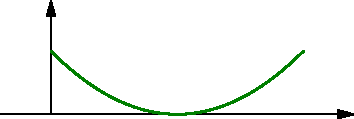
\includegraphics{Clebesg_4.pdf}
\caption{Cas 1. $M=g(a)=g(b)$}
\label{Clebesg_4}
\end{figure}

 La r{\'e}ciproque n'est pas vraie. Une relation $M=g(a)$ ou $g(b)$ n'emp{\^e}che pas que le maximum puisse {\^e}tre atteint en un autre point {\`a} l'int{\'e}rieur du segment. Dans ce cas $E$ ne sera pas $]a,b[ $. On peut choisir par exemple la fonction $\cos$ sur $[0,4\pi]$.
\begin{figure}[ht]
\centering
\includegraphics[width=7cm]{Clebesg_5.pdf}
\caption{Cas où $g(a)= M = g(B)$ et  $E$ n'est pas $]a,b[$.}
\end{figure}
\end{enumerate}
\end{enumerate}

\subsection*{Partie II}
\begin{enumerate}
 \item Quand $x$ augmente, l'intervalle $[ x,b] $ se r{\'e}duit. La fonction $\Psi $ est donc d{\'e}croissante.\newline
 Pour {\'e}tudier la continuit{\'e} de $\Psi$, deux méthodes sont possibles.\newline
La première consiste en une étude locale autour d'un point $x$ de $[a,b[ $.\newline
Remarquons d'abord que la fonction continue $g$ atteint sa borne sup{\'e}rieure sur $[x,b] $. Il existe donc $m\in [x,b]$ tel que $\Psi (x)=g(m)$. Distinguons deux cas.
\begin{description}
 \item[Cas 1.] $\Psi (x)=g(m)>g(x)$.\newline
Alors $m\in ] x,b] $ et par continuité en $x$,  il existe $\alpha >0$ tel que
\begin{displaymath}
 \forall t \in [x-\alpha,x]  : g(t)<g(m)
\end{displaymath}
On en d{\'e}duit que $\Psi(y)=\Psi(x)$ lorsque $y\in [x-\alpha ,m]$. Ainsi, la fonction $\Psi $ est non seulement continue mais \emph{constante} au voisinage de $x$.
\item[Cas 2.] $\Psi (x)=g(m)=g(x)$.\newline
Par continuit{\'e} de $g$ en $x$, pour tout $\varepsilon >0$, il existe un $\alpha >0$ tel que 
\begin{displaymath}
 \forall t\in [x-\alpha ,x+\alpha]  :  \Psi(x)-\varepsilon \leq g(t)\leq \Psi (x)+\varepsilon 
\end{displaymath}
On va alors chercher à encadrer $\Psi(y)$ pour $y\in [x-\alpha ,x+\alpha]$.\newline
Utilisons d'abord d{\'e}croissance de $\Psi$ :
\begin{displaymath}
\forall y\in [x-\alpha ,x+\alpha] : \Psi(x+\alpha )\leq \Psi(y)\leq \Psi (x-\alpha)
\end{displaymath}
D'un côté :
\begin{align*}
\forall t\in [ x-\alpha ,x] &:& g(t)\leq \Psi (x)+\varepsilon \\
\forall t\in [ x,b] &:& g(t)\leq \Psi (x)
\end{align*}
ce qui entra\^{\i }ne $\Psi (x-\alpha )\leq \Psi (x)+\varepsilon$.\newline
De l'autre 
\begin{displaymath}
 \Psi(x)-\varepsilon \leq g(x+\alpha)\leq \Psi(x+\alpha)
\end{displaymath}
ce qui entra\^{\i }ne $\Psi (x)-\varepsilon\leq \Psi(x+\alpha)$.\newline
Finalement on a donc 
\begin{displaymath}
 \forall y\in [x-\alpha ,x+\alpha] : \Psi (x)-\varepsilon\leq \Psi(x+\alpha) \leq \Psi(y)\leq \Psi (x-\alpha )\leq \Psi (x)+\varepsilon
\end{displaymath}
ce qui assure la continuité de $\Psi$ en $x$.
\end{description}
Une deuxième méthode possible consiste à utiliser un résultat de cours sur les fonctions monotones. Si $f$ est une fonction monotone définie sur un intervalle $I$ et si $f(I)$ est un intervalle, alors $f$ est continue dans $I$. Ce résultat repose sur l'étude des limites des fonctions monotones. Il sert en particulier à prouver la continuité de la bijection réciproque d'une fonction bijective, monotone et continue sur un intervalle.\newline
Il faudrait alors montrer que l'image par $\psi$ de l'intervalle $[a,b]$ est un intervalle.\newline
La fonction $g$ est continue sur un segment donc bornée. Notons
\begin{displaymath}
 M=g(x_m)=\max_{[a,b]}g
\end{displaymath}
Il est clair que $\Psi$ est à valeurs dans $[M,g(b)]$. On doit montrer que, pour tout $y$ dans $[M,g(b)]$, il existe un $x\in [a,b]$ tel que $\Psi(x)=y$. Cette méthode ne sera pas développée davantage.

\item \begin{enumerate}
 \item Un {\'e}l{\'e}ment $x$ de $] a,b[ $ est dans $E$ si et seulement si $g(x)<\Psi (x)$.
 
 \item Si $x\in E$, on sait que 
\begin{displaymath}
\dfrac{\Psi (x)-g(x)}{2}>0 
\end{displaymath}
En prenant cette quantit{\'e} comme $\varepsilon $ et en {\'e}crivant
la d{\'e}finition des continuit{\'e}s de $g$ et de $\Psi $ en $x$, on obtient facilement l'inclusion demand{\'e}e.
\end{enumerate}
\item \begin{enumerate}
 
  \item Notons $M_x$ la partie de $\R$ dont $s(x)$ est la borne inférieure :
\begin{displaymath}
 M_{x} = \left\lbrace  \xi \in \left] x,b \right] \text{ tq } g(x) < g(\xi ) \right\rbrace.
\end{displaymath}
C'est une partie non vide (car $x\in E$) de $]x,b]$, sa borne inf{\'e}rieure $s(x)$ est donc un {\'e}l{\'e}ment de $[x,b] $.\newline
Il est impossible que $s(x)=b$. En effet on aurait alors $M_{x}= \left\lbrace b \right\rbrace$ donc $g(x) < g(b)$. Dans ce cas, la continuit{\'e} de $g$ en $b$ entra\^{\i }nerait $g(x)<g(y)$ pour $y$ assez proche de $b$. Ceci serait en contradiction avec $M_{x}=\left\lbrace b\right\rbrace $.\newline
On doit donc avoir $s(x) \in \left[ x,b \right[$.
\newline Si $y\in \left[ x,s(x) \right[$, par définition d'une borne inférieure, $y$ n'est pas un {\'e}l{\'e}ment de $M_{x}$ donc $g(y)\leq g(x)$.

  \item Comme $g$ est continue en $s(x)$, la limite de $g(y)$ quand $y \rightarrow s(x)$ dans $[x,s(x)[ $ est $g(s(x))$. Par passage {\`a} la limite dans une in{\'e}galit{\'e} :
\begin{displaymath}
 g(s(x))\leq g(x)
\end{displaymath}
Lorsque $n$ est assez petit pour que $s(x)+\frac{1}{n}<b$, le nombre $s(x)+ \frac{1}{n}$ n'est pas un minorant de $M_{x}$, il existe donc $\xi_{n}\in M_x$ tel que
\[s(x) \leq \xi_{n}<s(x)+\frac{1}{n}\]
La suite des $\xi _{n}$ converge vers $s(x)$ en v{\'e}rifiant $g(x)<g(\xi _{n})$. Par passage {\`a} la limite :
\begin{displaymath}
g(x)\leq g(s(x)) 
\end{displaymath}
et finalement 
\begin{displaymath}
 g(x)=g(s(x))
\end{displaymath}
Pour tout $y\in [x,s(x)[$, $y$ n'est pas un élément de $M_x$, donc
\begin{displaymath}
 g(y)\leq g(x)
\end{displaymath}
 De plus pour tous les $\xi\in M_x$ :
\begin{displaymath}
 g(x)<g(\xi )
\end{displaymath}
On a donc prouvé l'existence d'un $\xi$ tel que :
\begin{displaymath}
 y<s(x)\leq \xi \leq b, \hspace{1cm}
g(y)\leq g(x) < g(\xi).
\end{displaymath}
Ce qui assure que $y$ est un {\'e}l{\'e}ment de $E$.
\end{enumerate}
\end{enumerate}
%
\newpage%
\section*{Problème 18}%
\addcontentsline{toc}{section}{Pb 18 : Nombres complexes et fonctions usuelles : autour de la formule de Machin.}%
\fancyhead[LO,RE]{Corrigés - Pb 18 : Nombres complexes et fonctions usuelles : autour de la formule de Machin.}%
\subsection*{Partie I}
\begin{enumerate}
\item Exprimons d'abord $x$ puis $x+i$:
\begin{displaymath}
 \alpha=\arctan \frac{1}{x} \Rightarrow x=\frac{\cos \alpha}{\sin \alpha}\\
\Rightarrow x+i=\frac{1}{\sin \alpha}e^{i\alpha}
\end{displaymath}
Deux expressions sont possibles pour les arguments de $x+i$.
\begin{align*}
 x>0 \Rightarrow \alpha\in ]0,\frac{\pi}{2}[ \Rightarrow \sin \alpha >0 &:& \alpha \text{ est un argument de } x+i\\
 x<0 \Rightarrow \alpha\in ]-\frac{\pi}{2},0[ \Rightarrow \sin \alpha <0 &:& \alpha +\pi \text{ est un argument de } x+i 
\end{align*}
Dans les deux cas, $\alpha$ est congru modulo $2\pi$ à un argument de $x+i$.
\item Posons $\beta = \arctan \frac{1}{y}$. Un calcul analogue à celui de la question précédente conduit à :
\[(x+i)^m(y+i)e^{-i\frac{\pi}{4}}=\frac{1}{\sin^m \alpha \sin \beta}e^{i(m\alpha +\beta -\frac{\pi}{4})}\]
Ce nombre complexe est réel si et seulement si
\[m\alpha +\beta -\frac{\pi}{4} \equiv 0 \quad (\pi)\]

\item On calcule $(2+i)^2(-7+i)$ et on trouve $-25(1+i)$. On en déduit la formule demandée modulo $\pi$. Pour lever cette ambigüité à $\pi$ près, on remarque que
\[0<\arctan\frac{1}{7}<\arctan\frac{1}{2}<\frac{\pi}{4}\]
donc
\begin{eqnarray*}
0<\arctan\frac{1}{2}-\arctan\frac{1}{7}<\frac{\pi}{4}\\
0<\arctan\frac{1}{2}<\frac{\pi}{4}
\end{eqnarray*}
La somme est donc bien entre $0$ et $\frac{\pi}{2}$.

\item En developpant et en utilisant $rq-1=p^2$, on obtient
\[(p+r+i)(p+q+i)=(2p+q+r)(p+i)\]
L'égalité en découle à un multiple de $\pi$ près. De plus, les deux membres de l'égalité sont entre $0$ et $\pi$, ils sont donc forcément égaux.
\end{enumerate}

\subsection*{Partie II}
\begin{enumerate}
\item En utilisant des formules du binôme et en séparant les parties réelles et imaginaires, on obtient

\begin{center}
\renewcommand{\arraystretch}{1.5}
\begin{tabular}{c|c|c|c|c}
 $m$ & 1 & 2 & 3 & 4\\ \hline
 $A_m$ & $x$ & $x^2-1$ & $x^3-3x$ & $x^4-6x^2+1$\\\hline
 $B_m$ & 1 & $2x$ & $3x^2-1$ & $4x^3-4x$
\end{tabular}  
\end{center}

\item Il s'agit de séparer les parties réelles et imaginaires de
\begin{displaymath}
 A_{m+1}+iB_{m+1} = (A_m+iB_m)(x+i)
\end{displaymath}
On obtient :
\begin{align*}
A_{m+1} =xA_m-B_m & & B_{m+1}= A_m+xB_m
\end{align*}
Ici encore, on sépare les parties réelles et imaginaires après quelques manipulations simples :
\begin{multline*}
 A_m(-x)+iB_m(-x) = (-x+i)^m = (-1)^m (x-i)^m 
= (-1)^m \overline{(x+i)^m} \\
= (-1)^m(A_m-iB_m)
\end{multline*}
On en déduit :
\begin{align*}
 A_m(-x)=(-1)^mA_m(x) & & B_m(-x)=-(-1)^mB_m(x)
\end{align*}
Cette fois on dérive 
\begin{displaymath}
 (A_m+iB_m)' = m(x+i)^{m-1}
\end{displaymath}
\begin{align*}
 A'_m = mA_{m-1} & & B'_m = mB_{m-1}
\end{align*}
Pour $x\neq0$, on fait apparaitre $\frac{1}{x}$
\begin{displaymath}
 (x+i)^m = (ix)^m \left(\frac{1}{i}+\frac{1}{x} \right)^m
= (-ix)^m \left(i-\frac{1}{x} \right)^m
\end{displaymath}
Si $m$ est pair :
\begin{displaymath}
 (-i)^m =(-1)^\frac{m}{2} \Rightarrow
\left\lbrace 
\begin{aligned}
 A_m(x) &= (-1)^\frac{m}{2}x^m A_m(-\frac{1}{x})\\
 B_m(x) &= (-1)^\frac{m}{2}x^m B_m(-\frac{1}{x})
\end{aligned}
\right. 
\end{displaymath}
Si $m$ est impair :
\begin{multline*}
 (-i)^m = -(-1)^\frac{m-1}{2}i 
\Rightarrow
(x+i)^m= -(-1)^\frac{m+1}{2}i x^m \left(A_m(-\frac{1}{x})+iB_m(-\frac{1}{x}) \right) \\
= (-1)^\frac{m-1}{2} x^m\left(B_m(-\frac{1}{x}) - iA_m(-\frac{1}{x}) \right)
\\
\Rightarrow
\left\lbrace 
\begin{aligned}
 A_m(x) &= (-1)^\frac{m-1}{2}x^m B_m(-\frac{1}{x})\\
 B_m(x) &= -(-1)^\frac{m-1}{2}x^m A_m(-\frac{1}{x})
\end{aligned}
\right. 
\end{multline*}

\item En utilisant $\arctan$ pour exprimer un argument de $x+i$, on peut écrire une suite d'équivalences :
\begin{multline*}
 A_m(x)=B_m(x)\Leftrightarrow \frac{\pi}{4}\equiv  \text{ un argument de } (x+i)^m \mod(\pi)\\
\Leftrightarrow m\arctan\frac{1}{x} \equiv \frac{\pi}{4}  \mod(\pi) 
\Leftrightarrow \arctan\frac{1}{x} \equiv \frac{\pi}{4m} \mod(\frac{\pi}{4m})
\end{multline*}
On en déduit que l'ensemble des solutions est
\begin{displaymath}
 \left\lbrace 
\cotan \left(\frac{\pi}{4m}+k\frac{\pi}{m} \right)\;,\;k\in\{0,\cdots,m-1\} 
\right\rbrace 
\end{displaymath}
Tous les $\frac{(4k+1)\pi}{4m}$ sont dans $]0,\pi[$. La fonction $\cotan$ est décroissante dans cet intervalle. Donc la plus grande des solutions est
\begin{displaymath}
 \cotan\left( \frac{\pi}{4m}\right) 
\end{displaymath}

\item On calcule la dérivée de $F_m$ en remplaçant les dérivées des polynômes à l'aide des formules de la question II.2. et en utilisant les relations de récurrence pour n'avoir que des $m-1$. On obtient
\begin{displaymath}
 F'_m =
-2m \frac{A_{m-1}^2 + B_{m-1}^2}{(A_m - B_m)^2}
\end{displaymath}
On en déduit que $F_m$ est décroissante dans chaque intervalle de son domaine de définition. Il s'agit d'intervalles ouverts dont les extrémités sont les $\cotan \frac{(4k+1)\pi}{4m} $ pour $k$ entre $0$ et $m-1$.\newline
D'après la formule du binôme, le degré de $A_m$ est $m$ et celui de $B_m$ est $m-1$ donc $F_m$ tend vers $+1$ en $+\infty$ et $-\infty$.
\end{enumerate} 

\subsection*{Partie III. Les formules du type Machin}
\begin{enumerate}
 \item D'après la définition, $(x,y)\in\mathcal C_m$ si et seulement si  
\begin{displaymath}
 (x+i)^m(y+i)\in\R e^{i\frac{\pi}{4}}
\end{displaymath}
Un nombre complexe est dans $\R e^{i\frac{\pi}{4}}$ si et seulement si sa partie réelle est égale à sa partie imaginaire. Or
\begin{multline*}
 (x+i)^m(y+i)=(A_m(x)+iB_m(x))(y+i) \\
 = A_m(x)y-B_m(x)+i(B_m(x)y+A_m(x))
\end{multline*}
Donc
\begin{multline*}
 (x,y)\in C_m \Leftrightarrow A_m(x)y-B_m(x) = B_m(x)y+A_m(x) \\
\Leftrightarrow (A_m(x)-B_m(x))y = A_m(x) + B_m(x)
\end{multline*}
On en déduit :
\begin{displaymath}
 \left.  
\begin{aligned}
 A_m(x) &\neq B_m(x)\\
 y &=F_m(x) 
\end{aligned}
\right\rbrace
\Rightarrow (x,y)\in \mathcal C_m
\end{displaymath}
Supposons maintenant $(x,y)\in \mathcal C_m$ avec $A_m(x) = B_m(x)$. Alors $A_m(x)+B_m(x)=0$ donc $A_m(x)=B_m(x)=0$ donc $(x+iy)^m$  devrait aussi être nul ce qui est évidemment faux car $x$ et $y$ sont non nuls. Ceci montre l'implication réciproque. 
\item Ici, $m$ désigne un entier entre $1$ et $4$.\newline
Les fonctions $F_m$ sont strictement décroissantes dans leurs intervalles de définition et tendent vers $1$ en $+\infty$.\\
D'après le tableau des valeurs de $\cotan\frac{\pi}{4m}$, la plus grande de ces valeurs est inférieure à $6$. On est donc certain que l'intervalle $[13,+\infty[ $ est tout entier dans un intervalle de définition de $F_m$. Comme $F_m(13)$ est strictement inférieur à $2$ et que $F_m$ tend vers $1$ à l'infini, on est certain qu'aucun $F_m(x)$, pour $x\geq 14$, ne peut prendre de valeur entière.\newline
On peut lire sur les tableaux les entiers entre $1$ et $13$ pour lesquels les $F_m(x)$ prennent des valeurs entières.\newline
Pour $m=1$ :
\begin{align*}
 &x=2  &y=F_1(2)=3 & & \arctan \frac{1}{2}+\arctan\frac{1}{3} \equiv \frac{\pi}{4} \hspace{10pt} (\pi)\\
 &x=3  &y=F_1(3)=2 & & \text{ même formule }
\end{align*}
Ici, les deux $\arctan$ sont entre $0$ et $\frac{\pi}{2}$ donc leur somme est entre $0$ et $\pi$ donc
\begin{displaymath}
 \arctan \frac{1}{2}+\arctan\frac{1}{3} = \frac{\pi}{4}
\end{displaymath}
Pour $m=2$ :
\begin{align*}
 x=&1 & & y = F_2(1)=-1 & & 2\arctan 1 + \arctan (-1) = \frac{\pi}{4}&\hspace{20pt}\text{ (évident)}\\
 x=&2 & & y = F_2(2)=-7 & & 2\arctan\frac{1}{2} - \arctan\frac{1}{7} = \frac{\pi}{4}& \\
 x=&3 & & y = F_2(3)=7  & & 2\arctan\frac{1}{3} + \arctan\frac{1}{7} = \frac{\pi}{4}&
\end{align*}
On a fait disparaitre le modulo $\pi$ par une évaluation numérique.
\end{enumerate}
Pour $m=3$, il n'existe pas de formule de Machin.\newline
Pour $m=4$, on obtient \emph{la} formule de Machin:
\begin{align*}
 x&=5 & y&=F_4(5)=-239 & 4\arctan\frac{1}{5} - \arctan\frac{1}{239}=\frac{\pi}{4}
\end{align*}
On a fait disparaitre le modulo $\pi$ par une évaluation numérique.

\subsection*{Partie IV. Algorithme de Lehmer.}
\begin{enumerate}
 \item Les calculs conduisent à :
\begin{align*}
 z_0&= 17+7i & & z_1=-41+3i & & z_2=-577+i & & z_4=-33290
\end{align*}
\item Pour un entier $k$  tel que $z_k$ est défini et de partie imaginaire strictement positive, notons $a_k$ et $b_k$ respectivement sa partie réelle et sa partie imaginaire. Montrons que 
\begin{displaymath}
 0\leq b_{k+1} < b_{k} 
\end{displaymath}
Par définition:
\begin{displaymath}
 z_{k+1}=(-n_k +i)(a_k +ib_k)
=-n_ka_k-b_k +i(-n_kb_k+a_k)
\Rightarrow
\left\lbrace 
\begin{aligned}
b_{k+1} &= a_k-n_kb_k \\
a_{k+1} &= -n_k-b_k
\end{aligned}
\right. 
\end{displaymath}
Par définition de la partie entière :
\begin{multline*}
 n_k\leq \frac{a_k}{b_k} <n_k +1 
\Rightarrow n_kb_k\leq a_k <n_kb_k + b_k \\
\Rightarrow 0 \leq a_k -n_kb_k<b_k
\Rightarrow 0\leq b_{k+1} <b_k
\end{multline*}

\item \begin{enumerate}
 \item Lorsque $a_0$ et $b_0$ sont des entiers, les relations obtenus dans la question précédentes montrent que tous les $a_k$ et $b_k$ sont entiers. La suite des $b_k$ est une suite décroissante d'entiers strictement positifs. Elle ne peut être infinie. Il existe donc un $k$ tel que $z_k$ est réel.
\item L'algorithme permet d'écrire 
\begin{align*}
 z_1 &= z_0(-n_0 + i)\\
z_2 &= z_1(-n_1+i)\\
 &\vdots \\
z_k &= z_{n-1}(-n_{k-1}+i)\in \R
\end{align*}
d'où
\begin{displaymath}
 \frac{z_k}{z_0} = (-n_0 + i)(-n_1 + i)\cdots (-n_{k-1} + i)
\end{displaymath}
Comme $z_k$ est réel, les arguments de $\frac{1}{z_0}$ et de $(-n_0 + i)\cdots (-n_{k-1} + i)$ sont congrus modulo $\pi$.\newline
Pour $w$ complexe de partie imaginaire strictement positive, un argument est :
\begin{align*}
 &\arctan\left( \frac{\Im w}{\Re w}\right)  &\text{ si } \Re w >0 \\
 &\arctan\left( \frac{\Im w}{\Re w}\right) +\pi &\text{ si } \Re w <0 \\
 &\frac{\pi}{2} &\text{ si } \Re w =0
\end{align*}
Les arguments de $z_0$ sont donc congrus modulo $\pi$ à $\arctan \frac{b}{a}$, ceux de $-n_j+i$ à $-\arctan \frac{1}{n_j}$ (ou $\frac{\pi}{2}$ si $n_j=0$). On en déduit :
\begin{displaymath}
 -\arctan \frac{b}{a}\equiv
\left( -\arctan \frac{1}{n_0}\right) + \cdots +\left( -\arctan \frac{1}{n_0}\right) \hspace{20pt} (\pi)
\end{displaymath}
Ce qui donne la formule annoncée en remplaçant éventuellement certains termes par des $\frac{\pi}{2}$.
\end{enumerate}

\end{enumerate}
%
\newpage%
\section*{Problème 19}%
\addcontentsline{toc}{section}{Pb 19 : Chemins et nombres de Catalan.}%
\fancyhead[LO,RE]{Corrigés - Pb 19 : Chemins et nombres de Catalan.}%
Avec les définitions, le $m(\Gamma)$ pour l'exemple de la figure vaut $1$.
\begin{enumerate}
 \item 
\begin{enumerate}
 \item Quand sur un chemin, on passe d'un point au point suivant, une seule des deux coordonnées augmente de $1$. Pour aller de $(0,0)$ à $(n,n)$, les deux coordonnées doivent augmenter de $n$. La longueur d'un chemin dans $\mathcal{P}_{0,n}$ est donc $2n$. 
 \item Montrons que 
\begin{displaymath}
\sharp\,\mathcal{P}_{0,n} = \binom{2n}{n} 
\end{displaymath}
en formant une bijection avec l'ensemble des parties de $\llbracket 1,2n \rrbracket$.\newline
Définissons une application de $\mathcal{P}(\llbracket 1,2n \rrbracket)$ dans $\mathcal{P}_{0,n} $ en associant à une partie $\Omega$ de $\llbracket 1,2n \rrbracket$ un chemin $\Gamma_\Omega=(M_0,M_1,\cdots,M_{2n})$. on pose $M_0=(0,0)$ et
\begin{displaymath}
\forall k\in \llbracket 1,2n \rrbracket,\;
M_k=
\left\lbrace  
\begin{aligned}
 &M_{k-1}+(1,0) &\text{ si } k\in \Omega \\
 &M_{k-1}+(0,1) &\text{ si } k\notin \Omega 
\end{aligned}
\right. 
\end{displaymath}
Pour tout chemein $\Gamma$, il existe une unique partie $\Omega$ telle que $\Gamma=\Gamma_\Omega$. Elle est formée avec les indices des points qui sont les extrémités droites des segments horizontaux du chemin.
\end{enumerate}

 \item 
\begin{enumerate}
 \item L'ensemble $\mathcal{C}_{0,1}$ contient un seul chemin $((0,0),(1,0),(1,1))$ donc $c_1=1$.\newline
L'ensemble $\mathcal{C}_{0,2}$ contient deux chemins seulement:
\begin{displaymath}
 ((0,0),(1,0),(1,1),(2,1),(2,2))\text{ et } ((0,0),(1,0),(2,0),(2,1),(2,2))
\end{displaymath}
donc $c_2=2$.
 \item La translation de vecteur $(-a,-a)$ définit une bijection de $\mathcal{P}_{a,b}$ vers $\mathcal{P}_{0,b-a}$. On en déduit
\begin{displaymath}
 \sharp\,\mathcal{C}_{a,b} = c_{b-a}
\end{displaymath}

 \item Si $(M_0,M_1,\cdots,M_{2m}$ est un chemin au dessous de la diagonale, on a forcément $M_1=(1,0)$ et $M_{2m-1}=(m,m-1)$. Lorsque les $M_1,\cdots,M_{2m-1}$ sont tous strictement au dessous de la diagonale, on peut les translater de $1$ vers la gauche en restant au dessous de la diagonale. Posons
\begin{displaymath}
 \forall i\in \llbracket 0, 2m-2 \rrbracket,\;
P_i = M_{i+1} -(1,0)
\end{displaymath}
On obtient une bijection de $\mathcal{C}'_{0,m}$ vers $\mathcal{C}_{0,m-1}$. On en déduit
\begin{displaymath}
 \sharp\,\mathcal{C}'_{0,m} = c_{m-1}
\end{displaymath}
 \item Par définition, $m$ prend ses valeurs entre $1$ et $n$ pour des chemins $\mathcal{C}_{0,n}$. Classons donc ces chemins suivant la valeur prise par la fonction $m$. On forme une partition
\begin{displaymath}
 \mathcal{C}_{0,n} = \mathcal{A}_1\cup \mathcal{A}_2\cup \cdots \cup \mathcal{A}_n 
\end{displaymath}
 où $\mathcal{A}_k$ est l'ensemble des chemins $\Gamma \in\mathcal{C}_{0,n}$ tels que $m(\Gamma)=k$.\newline
Si $\Gamma=(M_0,\cdots,M_{2n})$ est un tel chemin, on a $M_{2k}=(k,k)$ et, à cause de la minimalité dans la définition de $m$,
\begin{displaymath}
 (M_0,\cdots,M_{2k})\in \mathcal{C}'_{0,k},\hspace{1cm} (M_2k,\cdots,M_{2n})\in \mathcal{C}_{k,m}
\end{displaymath}
L'application
\begin{displaymath}
 \left\lbrace 
\begin{aligned}
 \mathcal{A}_{k} &\rightarrow \mathcal{C}'_{0,k}\times \mathcal{C}_{k,n} \\
 (M_0,\cdots,M_{2n}) &\mapsto \left( (M_0,\cdots,M_{2k}) , (M_{2k},\cdots,M_{2n})\right) 
\end{aligned}
\right. 
\end{displaymath}
est une bijection. On en déduit que $\sharp\,\mathcal{A}_k=c_{k-1}c_{n-k}$ d'après les questions b. et c. La partition de $\mathcal{C}_{0,n} $ conduit alors au résultat demandé. En remplaçant $n$ par $n+1$ et en utilisant $k-1$ comme nouvel indice, on obtient
\begin{displaymath}
 c_{n+1} = \sum_{k=0}^n c_kc_{n-k}
\end{displaymath}

\end{enumerate}

 \item 
\begin{enumerate}
 \item Posons $i=n-k$ dans la somme définissant $T_n$.
\begin{displaymath}
 T_n = \sum_{i=0}^n (n-i)a_{n-i}a_i= n\sum_{i=0}^n a_{n-i}a_i - \sum_{i=0}^n ia_{n-i}a_i
= nS_n - T_n
\end{displaymath}
 On en déduit $2T_n = nS_n$ puis
\begin{displaymath}
 T_{n+1}+S_{n+1} = \left( \frac{n+1}{2}+1\right) S_{n+1}=\frac{n+3}{2}S_{n+1}
\end{displaymath}

 \item D'après les définitions de l'énoncé et les propriétés des coefficients du binome,
\begin{displaymath}
 a_k=\frac{(2k)!}{k!(k+1)!},\hspace{0.5cm}
 a_{k+1}=\frac{(2k+2)!}{(k+1)!(k+2)!},\hspace{0.5cm}
 (k+1)a_{k+1}=\frac{(2k+2)!}{(k+1)!(k+1)!}
\end{displaymath}
D'autre part,
\begin{displaymath}
 2(2k+1)a_k=\frac{2(2k+1)!}{k!(k+1)!} = \frac{2(k+1)(2k+1)!}{(k+1)k!(k+1)!}=\frac{(2k+2)!}{(k+1)!(k+1)!}
\end{displaymath}
ce qui démontre l'égalité demandée. On en tire
\begin{multline*}
 T_{n+1}+S_{n+1}=a_{n+1}+\sum_{k=1}^{n+1}(k+1)a_ka_{n+1-k}\\
= a_{n+1}+\sum_{k=0}^{n}(k+2)a_{k+1}a_{n-k} \text{ (avec un changement d'indice  $k'=k-1$)}\\
= a_{n+1}+\sum_{k=0}^{n}2(2k+1)a_{k}a_{n-k} \text{ (avec la dernière relation) }\\
= a_{n+1} + 4T_n +2S_n \text{ (par définition de $T_n$ et $S_n$)}
\end{multline*}

 \item On suppose $S_n = a_{n+1}$. D'après a. et b.
\begin{displaymath}
 a_{n+1}+4T_n+2S_n = \frac{n+3}{2}S_{n+1}
\end{displaymath}
Exprimons $T_n$ en fonction de $S_{n+1}$ puis de $a_{n+2}$.
\begin{multline*}
 a_{n+1}+2(n+1)S_n= \frac{n+3}{2}S_{n+1} \Rightarrow
(2n+3)a_{n+1} = \frac{n+3}{2}S_{n+1}\\
\Rightarrow 
S_{n+1} = \frac{2(2n+3)}{n+3}a_{n+1} = a_{n+2}
\end{multline*}
d'après la relation du b. prise avec $k=n+1$.
On en déduit par récurrence que les suites $\left( a_n\right) _{n\in \N}$ et $\left( a_n\right) _{n\in \N}$ vérifient les mêmes conditions initiales et la même relation de récurrence. Elles sont donc égales.
\end{enumerate}

\end{enumerate}
%
\newpage%
\section*{Problème 20}%
\addcontentsline{toc}{section}{Pb 20 : Exemples de produits infinis.}%
\fancyhead[LO,RE]{Corrigés - Pb 20 : Exemples de produits infinis.}%
\subsection*{I. Exemples}
\begin{enumerate}
\item  Comme 
\[
 p_{n}=\frac{2}{1}\cdot \frac{3}{2}\cdots \frac{n+1}{n}=n+1
\]
le produit infini diverge vers $+ \infty $.

 \item  La clé est la relation $\sin(2x) = 2 \sin(x) \cos(x)$. 
\[
\cos \frac{a}{2^{p}}\sin \frac{a}{2^{p}}=\frac{1}{2}\sin \frac{a}{2^{p-1}} 
\Rightarrow
p_{n}=\prod_{p=1}^{n}\frac{1}{2}\frac{\sin \frac{a}{2^{p-1}}}{\sin \frac{a}{2^{p}}}=\frac{1}{2^{n}}\frac{\sin a}{\sin \frac{a}{2^{n}}}
\]
De plus, $2^{n}\sin \frac{a}{2^{n}}\rightarrow a$ quand $n\rightarrow +\infty $. Donc $(p_{n})_{n\in \N}\rightarrow \frac{\sin a}{a}$.

 \item Ici encore une simplification télescopique multiplicative se produit.
\begin{multline*}
 u_k = \frac{(k-1)(k+1)}{k^2} \\\Rightarrow
 p_n = \frac{(1)(3)}{2^2} \frac{(2)(4)}{3^2}\cdots \frac{(k-1)(k+1)}{k^2} \cdots \frac{(n-1)(n+1)}{n^2}\\
  = \frac{(n+1)}{2n} \rightarrow \frac{1}{2}.
\end{multline*}

 \item Calculons $(1-a^{2})p_{n}$.
\begin{multline*}
(1-a^{2})p_{n}  = (1-a^{2})(1+a^{2})(1+a^{4})(1+a^{8})\cdots (1+a^{2^{n}})\\ 
 = (1-a^{4})(1+a^{4})(1+a^{8})\cdots (1+a^{2^{n}}) \\
 = (1-a^{8})(1+a^{8})\cdots (1+a^{2^{n}}) 
 = \cdots  \\
 = (1-a^{2^{n}})(1+a^{2^{n}})=(1-a^{2^{n+1}})
\end{multline*}
On en d\'{e}duit que le produit infini converge vers $\frac{1}{1-a^{2}}$.

\end{enumerate}

\subsection*{II. Conditions.}
\begin{enumerate}
 \item  Si $(p_{n})_{n\in \N}$ converge vers $l\neq 0$, $(p_{n+1})_{n\in \N}$ converge aussi vers $l$ et \[(\frac{p_{n+1}}{p_{n}})_{n\in \N}=(u_{n+1})_{n\in \N}\] 
converge vers 1.

 \item Comme tous les $u_k$ sont strictement positifs à partir de $n_0$, on peut utiliser librement le logarithme et la fonction exponentielle qui sont toutes les deux continues.
\[
 (p_{n})_{n \geq n_0} \text{ converge } \Leftrightarrow (\frac{p_{n}}{p_{n_0-1}})_{n \geq n_0} \text{ converge } \Leftrightarrow (\ln(\frac{p_{n}}{p_{n_0-1}}))_{n \geq n_0} \text{ converge. }
\]
Or $\ln(\frac{p_{n}}{p_{n_0-1}} = \sum_{k=n_0}^{n}\ln(u_k)$. On en déduit
\[
 (p_{n})_{n \geq n_0} \text{ converge } \Leftrightarrow \left( \sum \ln(u_k) \right)_{k \geq n_0} \text{ converge.} 
\]
Dans le cas de convergence, on a
\[
 \prod_{n\geq 1} u_n = \left( \prod_{n\geq 1}^{n_0 -1} u_n\right)\, e^{\left( \sum_{n \geq n_0} u_n\right) } 
\]

 \item Les hypothèses traduisent le fait que la série des $\ln u_n$ est de signe constant à partir d'un certain rang. On peut donc appliquer les critères des séries à termes positifs. Si $u_n$ ne tend pas vers $1$, la série et le produit divergent grossièrement. Si la suite tend vers $1$ alors $v_n$ tend vers $0$ et $\ln(1\pm v_n)\sim \pm v_m$. La série des $\ln(u_n)$ converge si et seulement si la série des $v_n$ converge.\newline
 On peut remarquer que dans le cas où les $u_k$ sont plus petits que $1$ à partir d'un certain rang, la suite des produits est décroissante et positive donc elle converge. Mais par définition, la convergence d'un produit infini exige une limite non nulle. En fait la série des $v_k$ diverge vers l'infini si et seulement si le produit des $u_k$ tend vers $0$. 
 \item
\begin{enumerate}
  \item  On veut appliquer le théorème des accroissements finis à la fonction
\[f\; : \; x \rightarrow (\ln x )^2\]
entre $p$ et $p+1$. \'Etudions les variations de la dérivée 
\[x\rightarrow 2\frac{\ln x}{x}\]
Comme
\[
\left( \frac{\ln x}{x}\right) ^{\prime }=\frac{1-\ln x}{x^{2}} < 0 \text{ pour } x > e,
\]
cette dérivée est décroissante dans $\left] 3,+\infty \right[ $. On en d\'{e}duit 
\[
\forall x\in \left[ p,p+1\right], \; \frac{\ln x}{x}\leq \frac{\ln p}{p}
\]
La formule demand\'{e}e traduit alors
\[0\leq f(p+1)-f(p)\leq (p+1 -p)f^\prime(p)\]

  \item  En sommant les inégalités du a., pour tout $p$ entre 3 et $n\geq 3$, on obtient 
\begin{multline*}
(\ln(n+1))^2 -(\ln(3))^2 \leq 2\left(S_n-\frac{\ln 2}{2} \right) \\ 
\Rightarrow
S_n \geq \frac{1}{2}(\ln(n+1))^2 + \frac{\ln 2 -(\ln(3))^2}{2}
\end{multline*}
Ce qui entra\^{i }ne que $(S_{n})_{n\in \N}$ et $(p_{n})_{n\in \N}$ divergent vers $+\infty $.
\end{enumerate}
\end{enumerate}

\subsection*{III. Une expression de $\sin$ comme produit infini.}
\begin{enumerate}
 \item 
\begin{enumerate}
 \item Pour $x$ fixé dans $]-1,+1[$ et $n \in \N^*$, les $\frac{2x}{x^2 - n^2}$ sont strictement négatifs. L'opposé du terme général est équivalent à $\frac{x^2}{n^2}$ qui est le terme général d'une série convergente. On pouvait aussi dire que la série est absolument convergente. 
 \item On se trouve dans le premier cas de la question II.3. Le produit infini est convergent car la série de terme général $\frac{x^2}{n^2}$ est convergente.
\end{enumerate}

 \item
\begin{enumerate}
 \item Après calculs, on trouve
\[
 \pi \cot(\pi t) = \frac{1}{t} - \frac{\pi^2}{3}t + o(t).
\]

 \item En $0$, comme $\sin x \sim x$, $\ln(\frac{sin \pi t}{\pi t})$ converge vers $0$. En revanche la fonction diverge vers $-\infty$ en $1$ et $-1$. On prolonge donc par continuité en une fonction $f$ continue
\[
 \forall t \in ]-1,+1[, \;
 f(t) =
 \left\lbrace 
 \begin{aligned}
  \ln\left(\frac{\sin \pi t}{\pi t} \right) &\text{ si } t\neq 0 \\
  0  &\text{ si } t = 0
 \end{aligned}
\right. .
\]
 
 \item Comme elle est composée de fonctions $\mathcal{C}^{\infty}$, la fonction est clairement $\mathcal{C}^{1}$ dans l'intervalle privé de $0$ et continue dans $]-1,1[$. Pour montrer qu'elle est $\mathcal{C}^{1}$ dans $]-1,1[$, d'après le théorème de la limite de la dérivée, il suffit de prouver que la dérivée dans l'ouvert privé de $0$ admet une limite fini en $0$. Or
\[
 \forall t \neq 0, \; f'(t) = 
\left(\frac{\cos(\pi t)}{t} -\frac{\sin(\pi t)}{\pi t^2} \right)\frac{\pi t}{\sin (\pi t)}
= \pi \cot(\pi t) - \frac{1}{t}
\sim - \frac{\pi^2}{3}t \rightarrow 0.
\]
La fonction $f$ est donc $\mathcal{C}^1$ avec 
\[
 f'(t) = 
\left\lbrace 
\begin{aligned}
 &0 &\text{ si } t = 0 \\
 &\pi \cot(\pi t) - \frac{1}{t} &\text{ si } t \neq 0
\end{aligned}
\right. 
\]
\end{enumerate}

 \item
\begin{enumerate}
 \item On calcule la différence
\[
 \frac{1}{n^2 -1} - \frac{t}{n^2 -t^2}= \frac{(n^2+t)(1-t)}{(n^2 -1 )(n^2 -t^2)} > 0.
\]

 \item Fixons un entier $N$ et notons $r_N$ le reste:
\[
 f'(x) = \sum_{k=1}^N\frac{2x}{x^2 - k^2} + r_N(x).
\]
La fonction $r_N$ qui s'exprime comme une différence est continue. On intégre entre $0$ et $x$ (pour $|x| < 1$) en utilisant la linéarité de l'intégrale
\[
 \ln\left(\frac{\sin \pi x}{\pi x} \right) = f(x) = \sum_{k=1}^N\int_0^x\frac{2t}{t^2 - k^2}\,dt + \underset{=R_N(x)}{\underbrace{\int_0^xr_N(t)\,dt}} \\
\]
Majorons $|R_N(x)|$. Commençons par 
\[
 |R_N(x)| \leq \int_0^{|x|}|r_N(t)|\,dt.
\]
$r_N(t)$ est le reste d'une série. On le majore (pour tous les $t$) avec l'inégalité de la question a. par un nombre \emph{indépendant} de $t$
\begin{multline*}
 |r_N(t)| = \underset{p\rightarrow +\infty}{\lim}\left| \sum_{k=N+1}^{p}\frac{2t}{t^2 - k^2}\right|
  \leq \underset{p\rightarrow +\infty}{\lim} \sum_{k=N+1}^{p}\left|\frac{2t}{t^2 - k^2}\right| \\
  \leq \underset{p\rightarrow +\infty}{\lim} \sum_{k=N+1}^{p} \frac{2}{k^2 -1}
\leq \sum_{k=N+1}^{+\infty} \frac{2}{k^2 -1}
\end{multline*}
Il reste à integrer cette fonction constante sur un intervalle de longueur $|x|$ pour obtenir l'inégalité demandée.

 \item Calculons les intégrales dans la somme
\[
 \sum_{k=1}^N\int_0^x\frac{2t}{t^2 - k^2}\,dt 
 =  \sum_{k=1}^{N}\ln \frac{k^2 - t^2}{k^2}
 = \ln\left( \prod_{k=1}^N (1-\frac{x^2}{k^2})\right) .
\]
On a vu que le produit infini est convergent. Le ajorant à droite est le reste d'une série convergente. On en déduit en passant à la limite
\[
 \ln\left(\frac{\sin \pi x}{\pi x} \right) = \ln\left( \prod_{k \geq 1} (1-\frac{x^2}{k^2})\right) 
 \Rightarrow \sin(\pi x) = \pi x \prod_{k \geq 1} (1-\frac{x^2}{k^2}).
\]
en composant par l'exponentielle (continue).
\end{enumerate}
\end{enumerate}
%
\newpage%
\section*{Problème 21}%
\addcontentsline{toc}{section}{Pb 21 : Introduction aux polynômes orthogonaux}%
\fancyhead[LO,RE]{Corrigés - Pb 21 : Introduction aux polynômes orthogonaux}%
\subsection*{Partie 1}
\begin{enumerate}
 \item 
 \begin{enumerate}
   \item Voir cours.
   \item Dans le cas particulier du produit scalaire défini par l'intégrale, on peut calculer directement les $c_n$.
\begin{displaymath}
 c_n = \int_{-1}^1 t^n dt = \left\lbrace 
% use packages: array
\begin{array}{ll}
0 & \mathrm{si}\: n \:\mathrm{impair} \\ 
\frac{2}{n+1} & \mathrm{si}\: n\: \mathrm{pair} 
 \end{array}
\right. 
\end{displaymath}
Le calcul direct des déterminants donne
\begin{eqnarray*}
 \Delta_1 = \frac{4}{3} &,& \Delta_2 = \frac{32}{135}
\end{eqnarray*}
Le calcul des polynômes $D_1$, $D_2$, $D_3$ donne :
\begin{displaymath}
 D_1 = 2X \:,\: D_2 = \frac{4}{3}(X^2-\frac{1}{3}) \:,\: D_3 = -\frac{32}{225}X + \frac{32}{135} X^3
\end{displaymath}
Le calcul de $D_3$ se fait par exemple en développant suivant la dernière colonne
\renewcommand{\arraystretch}{1.6}
\begin{displaymath}
 D_3 = \frac{2}{5}  
% use packages: array
\begin{vmatrix}
2 & 0 & \frac{2}{3} \\ 
\frac{2}{3} & 0 & \frac{2}{5} \\ 
1 & x & x^2
\end{vmatrix}
+\Delta_2 x^3
= \frac{2}{5}(-x)(\frac{4}{5}-\frac{4}{9})+\Delta_2 x^3
\end{displaymath}

 \end{enumerate}
\item Il est clair en développant selon la dernière ligne que chaque polynôme $D_n$ est de degré \emph{inférieur ou égal} à $n$ et que le coefficient de $X^n$ est $\Delta_{n-1}$.\newline
Pourquoi $\Delta_{n-1} \neq 0$ est-il non nul ?\newline
La matrice des $c_i$ (notons la $C$) est la matrice de la restriction du produit scalaire à l'espace des polynômes de degré inférieur ou égal à $n-1$ dans la base canonique. Il existe une base orthonormée pour cet espace, soit $P$ la matrice de passage entre la base canonique et la base orthonormée. On a alors $C=\trans P\,P$ donc $\Delta_{n-1}=(\det P)^2>0$.\newline
Pour montrer l'orthogonalité, considérons $(X^i/D_n)$ avec $i<n$. Notons
\begin{displaymath}
 D_n= a_0+a_1X + \cdots +a_n X^n
\end{displaymath}
où les coefficients sont obtenus par le développement selon la dernière ligne (en particulier $a_n=\Delta_n$). Par linéarité du produit scalaire :
\begin{displaymath}
 (X^i/D_n) = a_0c_i+a_1c_{i+1}+\cdots + a_nc_{i+n}
\end{displaymath}
On peut interpréter cette expression comme le développement d'un déterminant selon la dernière ligne
\begin{displaymath}
 (X^i/D_n) = \left \vert
\begin{array}{ccccc}
 c_0 & c_1 & \cdots & c_{n-1} & c_n \\
 c_1 & c_2 & \cdots & c_{n} & c_{n+1} \\
 \vdots & \vdots & \ddots & \vdots & \vdots \\
 c_{n-1} & c_n & \cdots & c_{2n-2} & c_{2n-1} \\
c_i & c_{i+1} & \cdots & c_{i+n-1} & c_{i+n}
\end{array}
\right \vert
\end{displaymath}
Ce dernier déterminant est nul car la même ligne (en $i$) se retrouve deux fois. Ceci assure, par linéarité, l'orthogonalité demandée.
\item
\begin{enumerate}
 \item Par définition, $P_n$ est orthogonal à $1,X,\cdots,X^{n-1}$. Il est donc orthogonal par linéarité à tout polynôme de degré inférieur ou égal à $n-1$. 
 \item Comme chaque $\lambda_n$ est non nul, chaque $\lambda_nP_n$ est bien de degré $n$. Il est clairement orthogonal aux $X^i$ par linéarité.
 \item Soit $\left( P_n\right) _{n\in \N}$ et $\left(Q_n\right) _{n\in \N}$ deux suites de polynômes orthogonaux. Ils sont tous les deux dans $\R_n[X]\cap \R_{n-1}[X]^\perp$. Cet espace est l'orthogonal dans $\R_n[X]$ de $\R_{n-1}[X]^\perp$ qui en est un hyperplan. Il est donc de dimension $1$. Les polynômes $P_n$ et $Q_n$ en sont chacun une base, ils sont donc colinéaires avec des coefficients non nuls.
\end{enumerate}
\item 
\begin{enumerate}
 \item Comme le coefficient de $x^n$ dans $D_n$ est $\delta_{n-1}$, on a $D_n=\Delta_{n-1}Q_n$.
 \item On peut écrire $Q_n=X^n +(Q_n-X^n)$ où $Q_n-X^n$ est de degré strictement inférieur à $n$ donc orthogonal à $Q_n$. On a donc :
\begin{displaymath}
 \Vert Q_n\Vert^2 = (Q_n/X^n+(Q_n-X^n))=(Q_n/X^n)
\end{displaymath}
Par un calcul de déterminant analogue à celui de la question 2, on obtient
\begin{displaymath}
 (D_n/X^n)=\Delta_n\Rightarrow \Delta_{n-1}(Q_n/X^n)=\Delta_n\Rightarrow 
\Vert Q_n\Vert^2 = \frac{\Delta_{n}}{\Delta_{n-1}}
\end{displaymath}
\end{enumerate}
\item Relation de récurrence
\begin{enumerate}
 \item Le polynôme $XP_n$ est de degré $n+1$, il s'exprime donc dans la base orthogonale $P_0,\cdots,P_{n+1}$:
\begin{displaymath}
 XP_n = \sum_{k=0}^n\frac{(XP_n/P_k)}{\Vert P_k\Vert^2}P_k
\end{displaymath}
En fait seules les trois dernières coordonnées ne sont pas nulles car, pour $k<n-1$,
\begin{displaymath}
 (XP_n/X_k)=(P_n/XP_k)= 0
\end{displaymath}
 d'après l'hypothèse sur le produit scalaire et par orthogonalité car $\deg(XP_k)=k+1<n$.
 \item D'après la question précédente, $XQ_{n-1}$ est une combinaison linéaire de $Q_{n-2}$, $Q_{n-1}$ et $Q_{n}$. La considération du terme de degré $n$ montre que le coefficient de $Q_n$ est égal à $1$. Si on note $-a_n$ et $-b_n$ les deux autres coefficients, on obtient bien
\begin{displaymath}
 Q_{n}=(X+a_n)Q_{n-1}+b_nQ_{n-2}
\end{displaymath}

\end{enumerate}
\end{enumerate}
\subsection*{Partie II.}
\begin{enumerate}
 \item On sait qu'il existe $\lambda_n\neq 0$ tel que $L_n=\lambda_nQ_n$. Pour assurer $L_n(1)=1$, on doit avoir 
\begin{displaymath}
L_n = \frac{1}{Q_n(1)}Q_n 
\end{displaymath}
 \item Posons $\Lambda_n(x)=L_n(-x)$. Il est clair que son degré est $n$. Par le changement de variable $t=-x$, on montre que $\left( \Lambda_n\right) _{n\in \N}$ est une famille de polynômes orthogonaux. Il existe donc des $k_n$ tels que $\Lambda_n = k_n L_n$. Que vaut $k_n$? Pour le savoir, considérons le terme de degré $n$ de $L_n$ avec son coefficient dominant $\lambda_n$. Par définition de $\Lambda_n$, ce terme est $\lambda_n(-x)^n = k_n\lambda_nx^n$ donc $k_n=(-1)^n$ ce qui prouve la relation demandée.

\item D'après la question 5.a.
\begin{displaymath}
 \beta_n = (XL_n/L_n)=\int_{-1}^{1}tL_n^2(t)dt = 0
\end{displaymath}
car la fonction $t\rightarrow tL_n^2(t)$ est impaire et le domaine d'intégration est symétrique.

 \item Comme $L_{n-1}$ et $L_n$ sont orthogonaux, à partir de l'expression de $XL_n$, on tire $(XL_n/L_{n-1})=\alpha_n\Vert L_{n-1}\Vert^2$. D'autre part, $(XL_n/L_{n-1})= (L_n/XL_{n-1})$.  Comme $XL_{n-1}$ est un polynôme de degré $n$ et de coefficient dominant $\lambda_{n-1}$, on peut écrire
\begin{multline*}
 XL_{n-1}=\frac{\lambda_{n-1}}{\lambda_n}L_n+\text{polynôme de degré $<n$ orthogonal à $L_n$}\\
\Rightarrow
(L_n/XL_{n-1})=(L_n/\frac{\lambda_{n-1}}{\lambda_n}L_n)
\Rightarrow
\alpha_n = \frac{\lambda_{n-1}}{\lambda_n}\frac{\Vert L_n\Vert^2}{\Vert L_{n-1}\Vert^2}
\end{multline*}
L'expression de $\gamma_n$ en fonction de $\lambda_n$ et $\lambda_{n-1}$ s'obtient simplement en considérant le coefficient dominant
\begin{displaymath}
 XL_n=\alpha_nL_{n-1}+\gamma_nL_{n+1}\Rightarrow 
\lambda_n = \gamma_n \lambda_{n+1}
\end{displaymath}

 \item Considérons $(L_n'/L_{n-1})$ et transformons cette expression par intégration par parties pour utiliser l'orthogonalité de $L_n$ avec $L_{n-1}'$ due au degré 
\begin{multline*}
 (L_n'/L_{n-1})=\int_{-1}^1L_n'(t)L_{n-1}(t)\,dt
=\left[L_n(t)L_{n-1}(t) \right]_{-1}^1- \int_{-1}^1L_n(t)L_{n-1}'(t)\,dt\\
=1 - (-1)^{n}(-1)^{n-1}-0=2
\end{multline*}
D'autre part, $L_n'$ est de degré $n-1$ et de coefficient dominant $n\lambda_n$. On peut donc écrire
\begin{multline*}
 L_n'= n\lambda_n X^{n-1} + \text{ polynôme de degré $< n-1$ orthogonal à $L_{n-1}$}\\
 = n \frac{\lambda_n}{\lambda_{n-1}}L_{n-1}+\text{ polynôme de degré $< n-1$ orthogonal à $L_{n-1}$}
\end{multline*}
ce qui entraine
\begin{displaymath}
 (L_n'/L_{n-1})=n \frac{\lambda_n}{\lambda_{n-1}}(L_{n-1}/L_{n-1})
\end{displaymath}
Des deux expressions obtenues, on tire
\begin{displaymath}
 2\lambda_{n-1}=n\lambda_n\Vert L_{n-1}\Vert^2
\end{displaymath}

 \item  On va d'abord exprimer les coefficients $\alpha_n$, $\beta_n$, $\gamma_n$ en fonction de $n$ et de la norme de $L_n$ puis exploiter la relation $\alpha_n+\beta_n+\gamma_n=1$ qui vient de ce que tous les $L_k$ prennent en $1$ la valeur $1$.\newline
D'après 4. et 5. :
\begin{displaymath}
 \left. 
\begin{aligned}
 \alpha_n = \frac{\lambda_{n-1}}{\lambda_n}\frac{\Vert L_n\Vert^2}{\Vert L_{n-1}\Vert^2}\\
 2\lambda_{n-1}=n\lambda_n\Vert L_{n-1}\Vert^2
\end{aligned}
\right\rbrace 
\Rightarrow
\alpha_n = \frac{n}{2}\Vert L_n \Vert^2
\end{displaymath}
On a montré en 3. que $\beta_n=0$. L'expression de $\gamma_n$ vient aussi de 4. et 5. (en décalant la relation tirée de 5.)
\begin{displaymath}
 \left. 
\begin{aligned}
 \gamma_n = \frac{\lambda_{n}}{\lambda_{n+1}}\\
 2\lambda_{n}=(n+1)\lambda_{n+1}\Vert L_{n}\Vert^2
\end{aligned}
\right\rbrace 
\Rightarrow
\gamma_n = \frac{n+1}{2}\Vert L_n \Vert^2
\end{displaymath}
On peut alors exprimer $\Vert L_n\Vert$:
\begin{displaymath}
\alpha_n+\beta_n+\gamma_n=1 \Rightarrow
\left(\frac{n}{2}+\frac{n+1}{2} \right)\Vert L_n\Vert^2=1 \Rightarrow
  \Vert L_n\Vert^2=\frac{2}{2n+1}
\end{displaymath}
On en déduit les valeurs de $\alpha_n$, $\beta_n$ et $\gamma_n$:
\begin{align*}
 \alpha_n=\frac{n}{2n+1}& &\beta_n=0 & & \gamma_n=\frac{n+1}{2n+1}
\end{align*}
puis la relation de récurrence
\begin{displaymath}
 XL_n=\frac{n}{2n+1}L_{n-1}+\frac{n+1}{2n+1}L_{n+1}
\end{displaymath}
qui s'écrit aussi
\begin{displaymath}
 L_{n+1}=\frac{2n+1}{n+1}XL_n-\frac{n}{n+1}L_{n-1}
\end{displaymath}

\end{enumerate}
%
\newpage%
\section*{Problème 22}%
\addcontentsline{toc}{section}{Pb 22 : Rotations, angles d'Euler, quaternions}%
\fancyhead[LO,RE]{Corrigés - Pb 22 : Rotations, angles d'Euler, quaternions}%
\subsection*{Partie I - Angles d'Euler}
\begin{enumerate}
 \item Par définition des rotations :
\begin{displaymath}
\left( r_2(\overrightarrow{i})=\overrightarrow{u}, \;
r_1(\overrightarrow{u})=\overrightarrow{u}, \;
r_3(\overrightarrow{u})=\overrightarrow{i_1}\right) 
\hspace{0.3cm} \Rightarrow \hspace{0.3cm}
r_3 \circ r_2 \circ r_1 (\overrightarrow{i})=\overrightarrow{i}
\end{displaymath}
De même 
\begin{displaymath}
 \left( r_2(\overrightarrow{k})=\overrightarrow{k}, \;
 r_1(\overrightarrow{k})=\overrightarrow{k_1},\;
 r_3(\overrightarrow{k_1})=\overrightarrow{k_1}\right) 
 \hspace{0.3cm} \Rightarrow \hspace{0.3cm}
r_3 \circ r_2 \circ r_1 (\overrightarrow{k})=\overrightarrow{k_1}. 
\end{displaymath}
La rotation composée transforme la base orthonormée directe $(\overrightarrow{i},\overrightarrow{j},\overrightarrow{k})$ en une base orthonormée directe $(\overrightarrow{i_1},\overrightarrow{w},\overrightarrow{k_1})$. La seule base orthonormée directe dont le premier et le troisième vecteur sont $\overrightarrow{i_1}$ et $\overrightarrow{k_1}$ est $(\overrightarrow{i_1},\overrightarrow{j_1},\overrightarrow{k_1})$. On en déduit
\begin{displaymath}
 r_3 \circ r_2 \circ r_1 = r
\end{displaymath}

\item La fonction $R=f\circ r_{\overrightarrow{w},\alpha}\circ f^{-1}$ est une rotation car elle est composée de plusieurs rotations (les rotations forment un groupe pour la composition). On va montrer que c'est une rotation d'angle $\alpha$ autour de l'axe $f(\overrightarrow{w})$.\newline
On vérifie facilement que $R(f(\overrightarrow{w}))=f(\overrightarrow{w})$. Pour montrer que l'angle est $\alpha$, on utilise la formule de changement de base.\newline
Soit $\mathcal U=(\overrightarrow{u},\overrightarrow{v},\overrightarrow{w})$ une base orthonormée directe et $\mathcal V=(f(\overrightarrow{u}),f(\overrightarrow{v}),f(\overrightarrow{w}))$. La famille $\mathcal V$ est également orthonormée directe car $f$ est une rotation. Alors:
\begin{displaymath}
\Mat_{\mathcal U} r_{\overrightarrow{w},\alpha} =
\begin{pmatrix}
 \cos \alpha & -\sin \alpha & 0 \\
 \sin \alpha & \cos \alpha & 0\\
0 & 0 & 1
\end{pmatrix}
\end{displaymath}
On peut alors regarder la matrice de $f$ comme une matrice de passage entre deux bases (elle exprime les vecteurs de $\mathcal V$ en fonction de ceux de $\mathcal U$) puis utiliser la formule de changement de base.
\begin{multline*}
 \Mat_{\mathcal U}f = P_{\mathcal V \mathcal U} \Rightarrow 
 \Mat_{\mathcal V}R=  P_{\mathcal U \mathcal V}\,\Mat_{\mathcal U}R\,P_{\mathcal V \mathcal U}\\
=P_{\mathcal U \mathcal V} 
    \left( \Mat_{\mathcal U}f \, \Mat_{\mathcal U}r_{\overrightarrow{w},\alpha} \, \Mat_{\mathcal U}f^{-1}\right) P_{\mathcal V \mathcal U}\\
= \left( P_{\mathcal U \mathcal V}\,P_{\mathcal V \mathcal U}\right)
  \Mat_{\mathcal U}r_{\overrightarrow{w},\alpha}
\left(  P_{\mathcal U \mathcal V}\,P_{\mathcal V \mathcal U} \right) 
=\Mat_{\mathcal U}r_{\overrightarrow{w},\alpha}
\end{multline*}
La forme de cette matrice montre que $R$ est la rotation d'angle $\alpha$ autour de $f(\overrightarrow{w})$.
\item On remarque que $r_\varphi$ et $r_\psi$ sont des rotations de même axe. Elles vont donc commuter. Comme $r_1$ et $R_\theta$ sont des rotations d'angle $\theta$ mais respectivement autour de $\overrightarrow{u}$ et $\overrightarrow{i}$ avec $\overrightarrow{u}=r_\varphi(\overrightarrow{i})$, la question précédente montre que
\begin{displaymath}
 r_1 = r_\varphi \circ R_\theta \circ r_\varphi ^{-1}
\end{displaymath}
De même, comme $r_1(\overrightarrow{k})=\overrightarrow{k_1}$ :
\begin{displaymath}
 r_3 = r_{\overrightarrow{k_1},\varphi}=r_1\circ r_\varphi \circ r_1^{-1}
\end{displaymath}
On en déduit :
\begin{multline*}
 r = r_3\circ r_1 \circ r_2 = r_1 \circ r_\psi \circ r_1^{-1}\circ r_1 \circ r_2 
= r_1 \circ r_\psi \circ r_2 \\
= r_\varphi \circ R_\theta \circ r_\varphi^{-1}\circ r_\psi \circ r\varphi 
=  r_\varphi \circ R_\theta \circ r_\psi
\end{multline*}
car $r_\varphi$ et $r_\psi$ commutent. Le point intéressant dans cette décomposition est que les axes des trois rotations soient dirigés par les vecteurs $\overrightarrow{i}$ et $\overrightarrow{k}$ de la base de départ.
\end{enumerate}

\subsection*{Partie II - Quaternions}
Les questions de cette partie se traitent par de simples vérifications. Leur correction ne sera pas détaillée.

\subsection*{Partie III - Multiplications}
\begin{enumerate}
 \item La vérification de ce que $S$, $g_q$, $d_q$, $C_q$ sont des endomorphismes ne pose pas de difficulté. Bien remarquer qu'il s'agit d'une structure de $\R$-espace vectoriel.\newline
Soit $q^\prime$ un quaternion quelconque, on peut écrire :
\begin{equation*}
 d_{q^{-1}}(q^\prime) = q^\prime q^{-1} = \dfrac{1}{N(q)}q^\prime \overline{q} = \dfrac{1}{N(q)}\overline{q\overline{q^\prime}}
\end{equation*}
donc
\begin{displaymath}
 d_{q^{-1}} = \dfrac{1}{N(q)} \,S \circ g_q \circ S
\end{displaymath}
De même :
\begin{displaymath}
 C_q=g_q \circ d_{q^{-1}}= \dfrac{1}{N(q)} \,g_q \circ S \circ g_q \circ S
\end{displaymath}
\item \begin{enumerate}
 \item Pour former la matrice de $g_q$, on exprime les images des vecteurs de base en fonction de $(1_{\mathbb{H}},\overrightarrow{i},\overrightarrow{j},\overrightarrow{k})$. On peut se permettre de ne pas écrire complètement certaines matrices car on \emph{sait} qu'il s'agit de quaternions.
\begin{displaymath}
 g_q(1)= \alpha 1_{\mathbb{H}} + \delta \overrightarrow{i} + \gamma \overrightarrow{j} + \beta \overrightarrow{k}
\end{displaymath}
\begin{multline*}
 g_q(\overrightarrow{i}) = 
 \begin{bmatrix}
a  & -\overline{b} \\
b  & \overline{a}
\end{bmatrix}
\begin{bmatrix}
0  & i \\
i  & 0 
\end{bmatrix}
=
\begin{bmatrix}
 -i\overline{b} & . \\
 i\overline{a} &  .
\end{bmatrix}
=
\begin{bmatrix}
 -i\gamma -\delta & . \\
 i\alpha + \beta & .
\end{bmatrix}
 \\
 = -\delta 1_{\mathbb{H}} + \alpha \overrightarrow{i} + \beta \overrightarrow{j}  -\gamma \overrightarrow{k}
\end{multline*}
\begin{multline*}
 g_q(\overrightarrow{j}) = 
 \begin{bmatrix}
a  & -\overline{b} \\
b  & \overline{a}
\end{bmatrix}
\begin{bmatrix}
0  & -1 \\
1  & 0 
\end{bmatrix}
=
\begin{bmatrix}
 -\overline{b} & . \\
 \overline{a} &  .
\end{bmatrix}
=
\begin{bmatrix}
 -\gamma +i\delta & . \\
 \alpha -i\beta & .
\end{bmatrix}
 \\
 = -\gamma 1_{\mathbb{H}} - \beta \overrightarrow{i} + \alpha \overrightarrow{j} + \delta \overrightarrow{k}
\end{multline*}
\begin{multline*}
 g_q(\overrightarrow{k}) = 
 \begin{bmatrix}
a  & -\overline{b} \\
b  & \overline{a}
\end{bmatrix}
\begin{bmatrix}
i  & 0 \\
0  & -i 
\end{bmatrix}
=
\begin{bmatrix}
 ia & . \\
 ib &  .
\end{bmatrix}
=
\begin{bmatrix}
 i\alpha -\beta & . \\
 i\gamma - \delta & .
\end{bmatrix}
 \\
 = -\beta 1_{\mathbb{H}} + \gamma \overrightarrow{i} - \delta \overrightarrow{j} + \alpha \overrightarrow{k}
\end{multline*}
On en déduit :
\begin{displaymath}
 \mathop{\mathrm{Mat}}_{\mathcal B}g_q = 
\begin{bmatrix}
 \alpha & -\delta & -\gamma & -\beta \\
 \delta & \alpha & -\beta & \gamma \\
 \gamma & \beta & \alpha & -\delta \\
 \beta & -\gamma & \delta & \alpha
\end{bmatrix}
\end{displaymath}
\item La matrice précédente s'écrit avec des blocs $2\times 2$ $A$, $B$ :
\begin{displaymath}
 \det g_q =
\begin{vmatrix}
A  & -B \\
B  & A 
\end{vmatrix}
\end{displaymath}
Ce déterminant n'est pas modifié par des opérations élémentaires sur les blocs :
\begin{multline*}
 \det g_q =
\begin{vmatrix}
A  & -B + iA \\
B  & A + iB 
\end{vmatrix}
= \begin{vmatrix}
A  & i(A + iB) \\
B  & A + iB 
\end{vmatrix}
= \begin{vmatrix}
A - iB  & 0 \\
B  & A + iB 
\end{vmatrix}
\\
=\vert \det(A+iB)\vert ^2
= \left\vert \begin{vmatrix}
\alpha + i\gamma  & -\delta + i\beta \\
\delta + i\beta  & \alpha - i\gamma 
\end{vmatrix} \right\vert ^2 
\\
= \vert (\alpha + i\gamma)(\alpha - i\gamma)-(\delta - i\beta)(\delta + i\beta)\vert^2
=(\alpha^2 + \beta^2 + \gamma^2 + \delta^2)^2 = N(q)^2
\end{multline*}
On en déduit :
\begin{displaymath}
 \det g_q = N(q)^2
\end{displaymath}
\end{enumerate}
\item L'égalité entre applications linéaires 
\begin{displaymath}
 C_q = \dfrac{1}{N(q)} g_q \circ S \circ g_q \circ S
\end{displaymath}
se traduit par l'égalité suivante entre les déterminants (attention, l'espace est de dimension $4$):
\begin{displaymath}
 \det C_q = \dfrac{1}{N(q)^4} (\det g_q)^2 (\det S)^2
\end{displaymath}
Or $(\det S)^2=1$ car $S\circ S$ est l'identité. On en déduit :
\begin{displaymath}
 \det C_q = 1
\end{displaymath}
\end{enumerate}

\subsection*{Partie IV - Produit scalaire}
Dans cette partie $\overrightarrow{u}$ et $\overrightarrow{v}$ sont deux quaternions purs respectivement de coordonnées $(\gamma , \delta , \beta)$ et $(\gamma^\prime , \delta^\prime , \beta^\prime)$ dans la base 
$(\overrightarrow{i} , \overrightarrow{j} , \overrightarrow{k})$.
\begin{align*}
 \overrightarrow{u} =&
\gamma \overrightarrow{i} +\delta \overrightarrow{j} + \beta \overrightarrow{k}
=
\begin{bmatrix}
i\beta  & -\gamma + i\delta \\
\gamma + i\delta  & -i\beta
\end{bmatrix}
\\
 \overrightarrow{v}
=& 
\gamma^\prime \overrightarrow{i} +\delta^\prime \overrightarrow{j} + \beta^\prime \overrightarrow{k}
=
\begin{bmatrix}
i\beta^\prime  & -\gamma^\prime + i\delta^\prime \\
\gamma^\prime + i\delta^\prime  & -i\beta^\prime
\end{bmatrix}
\end{align*}

\begin{enumerate}
 \item Pour vérifier que $(./.)$ définit un produit scalaire, formons le produit matriciel des quaternions.
\begin{displaymath}
 \overrightarrow{u}\overrightarrow{u^\prime} 
=
\begin{bmatrix}
-\beta \beta^\prime -\gamma \gamma^\prime -\delta \delta^\prime +i(\delta \gamma^\prime - \gamma \delta^\prime) & . \\
-\delta \beta^\prime + \beta \delta^\prime + i(\gamma \beta^\prime -\gamma^\prime \beta)  & .
\end{bmatrix}
\end{displaymath}
On en déduit l'expression du produit scalaire
\begin{displaymath}
 (\overrightarrow{u}/\overrightarrow{v}) = \dfrac{1}{2}\tr (\overrightarrow{u}\overrightarrow{v}) = 
\beta\beta^\prime + \gamma\gamma^\prime + \delta \delta^\prime
\end{displaymath}
Ceci montre en même temps que $(\overrightarrow{i}, \overrightarrow{j},\overrightarrow{k})$ est une base orthonormée. Elle est directe par définition de l'orientation de l'espace $E$ des quaternions purs.

\item Dans l'espace vectoriel euclidien oriené $E$, le calcul en coordonnées (dans une base orthonormée directe) du produit vectoriel $\overrightarrow{u}\overrightarrow{v}$ donne
\begin{displaymath}
 \begin{pmatrix}
  \delta \\
  \gamma \\
 \beta
 \end{pmatrix}
\wedge
 \begin{pmatrix}
  \delta^\prime \\
  \gamma^\prime \\
 \beta^\prime
 \end{pmatrix}
=
 \begin{pmatrix}
  \gamma \beta^\prime -\gamma^\prime \beta \\
  \beta \delta^\prime - \beta^\prime \delta \\
 \delta \gamma^\prime - \delta^\prime \gamma
 \end{pmatrix}
\end{displaymath}
On retrouve des expressions figurant dans le produit matriciel calculé plus haut, on en déduit :
\begin{displaymath}
\overrightarrow{u} \overrightarrow{v} = 
-(\overrightarrow{u}/\overrightarrow{v})1_{\mathbb H} + \overrightarrow{u} \wedge \overrightarrow{v}
\end{displaymath}
Les autres expressions demandées par l'énoncé en découlent immédiatement.
\end{enumerate}

\subsection*{Parties V - Rotations}
\begin{enumerate}
 \item \begin{enumerate}
 \item On doit montrer que l'image par l'application $C_q$ d'un quaternion pur $\overrightarrow{u}$ est encore un quaternion pur. On utilise la conjugaison (un quaternion est pur lorsqu'il est égal à l'opposé de son conjugué).
\begin{displaymath}
 C_q(\overrightarrow{u}) = \dfrac{1}{N(q)} q \overrightarrow{u} \overline{q}
\end{displaymath}
\begin{displaymath}
\overline{C_q(\overrightarrow{u})} = \dfrac{1}{N(q)} q \overline{\overrightarrow{u}} \overline{q} = \dfrac{1}{N(q)} q (-\overrightarrow{u}) \overline{q} = -C_q(\overrightarrow{u})
\end{displaymath}
On en déduit que $C_q(\overrightarrow{u})$ est un quaternion pur.
\item On note $c_q$ la restriction de $C_q$ à $E$. Comme $C_q(1_{\mathbb H}) = 1_{\mathbb H}$, la matrice de $C_q)$ dans la base $(1_{\mathbb H}, \overrightarrow i,\overrightarrow j,\overrightarrow k)$ est de la forme
\begin{displaymath}
 \begin{bmatrix}
  1 &  
\begin{matrix}
 0 & 0 & 0
\end{matrix}

\\
\begin{matrix}
 0 \\
 0 \\
 0
\end{matrix}
  & \mathop{\mathrm{Mat}}_{(\overrightarrow i,\overrightarrow j,\overrightarrow k)} c_q
 \end{bmatrix}
\end{displaymath}
D'après la définition du déterminant d'une matrice (ou en développant suivant la première colonne), on obtient
\begin{displaymath}
 \det c_q = \det C_q =1
\end{displaymath}
\item Comme $c_q$ est de déterminant 1, pour montrer que c'est une rotation, il suffit de montrer qu'il conserve le produit scalaire.
\begin{multline*}
 (c_q(\overrightarrow u)/c_q(\overrightarrow v)) = -\dfrac{1}{2} \tr (c_q(\overrightarrow u)c_q(\overrightarrow v))
= -\dfrac{1}{2} \tr (q \overrightarrow u q^{-1} q \overrightarrow v q^{-1}) \\
= -\dfrac{1}{2} \tr (q \overrightarrow u \overrightarrow v q^{-1}) 
= -\dfrac{1}{2} \tr (\overrightarrow u \overrightarrow v q^{-1} q) 
= -\dfrac{1}{2} \tr (\overrightarrow u \overrightarrow v )
= (\overrightarrow u / \overrightarrow v)
\end{multline*}
en utilisant le fait que la trace d'un produit de deux matrices ne change pas si on les permute 
\end{enumerate}
\item \begin{enumerate}
 \item Rappelons que
\begin{align*}
 q = \begin{bmatrix}
 a & -\overline{b} \\
 b & \overline{a}
     \end{bmatrix}
&,&
\overline{q} = \begin{bmatrix}
\overline{a}  & \overline{b} \\
 -b & a
\end{bmatrix}
\end{align*}
\begin{displaymath}
c_q(\overrightarrow i) = \dfrac{1}{N(q)} q 
\begin{bmatrix}
 0 & i \\
 i & 0
\end{bmatrix}
\overline{q}
= \dfrac{1}{N(q)} q 
\begin{bmatrix}
 -ib & ia \\
 i\overline{a} & i\overline{b}
\end{bmatrix} 
= \dfrac{1}{N(q)} 
\begin{bmatrix}
 . & . \\
 -ib^2+i\overline{a}^2 & 0
\end{bmatrix}
\end{displaymath}
\begin{displaymath}
 (c_q(\overrightarrow i)/\overrightarrow i) 
= \dfrac{\Im(-ib^2+i\overline{a}^2)}{N(q)}
=  \dfrac{\alpha^2 -\beta^2 -\gamma^2 +\delta^2}{N(q)}
\end{displaymath}

\begin{displaymath}
c_q(\overrightarrow j) = \dfrac{1}{N(q)} q 
\begin{bmatrix}
 0 & -1 \\
 1 & 0
\end{bmatrix}
\overline{q}
= \dfrac{1}{N(q)} q 
\begin{bmatrix}
 b & -a \\
 \overline{a} & \overline{b}
\end{bmatrix} 
= \dfrac{1}{N(q)} 
\begin{bmatrix}
 . & . \\
 b^2+\overline{a}^2 & 0
\end{bmatrix}
\end{displaymath}
\begin{displaymath}
 (c_q(\overrightarrow j)/\overrightarrow j)
= \dfrac{\Re(b^2+\overline{a}^2)}{N(q)}
= \dfrac{\gamma^2 -\delta^2 +\alpha^2 -\beta^2}{N(q)}
\end{displaymath}

\begin{displaymath}
c_q(\overrightarrow k) = \dfrac{1}{N(q)} q 
\begin{bmatrix}
 i & 0 \\
 0 & -i
\end{bmatrix}
\overline{q}
= \dfrac{1}{N(q)} q 
\begin{bmatrix}
 i\overline{a} & i\overline{b} \\
 ib & -ia
\end{bmatrix} 
= \dfrac{1}{N(q)} 
\begin{bmatrix}
 i|a|^2 -i|\overline{b}|^2 & . \\
 . & .
\end{bmatrix}
\end{displaymath}
\begin{displaymath}
 (c_q(\overrightarrow k)/\overrightarrow k)
= \dfrac{\Im(i|a|^2 -i|\overline{b}|^2)}{N(q)}
= \dfrac{\alpha^2 +\beta^2 -\gamma^2 -\delta^2}{N(q)}
\end{displaymath}
\item On déduit de la question précédente que
\begin{displaymath}
 \tr c_q = \dfrac{3\alpha^2 -\beta^2 -\gamma^2 -\delta^2}{\alpha^2 +\beta^2 +\gamma^2 +\delta^2}
\end{displaymath}
Cette trace est égale à 3 si et seulement si
\begin{displaymath}
 3\alpha^2 -\beta^2 -\gamma^2 -\delta^2 = 3(\alpha^2 +\beta^2 +\gamma^2 +\delta^2)
\end{displaymath}
c'est à dire lorsque $\beta^2 +\gamma^2 +\delta^2=0$ ou encore que $q\in \Vect (1_{\mathbb H})$.
\end{enumerate}
\item Lorsque $q\not\in \Vect (1_{\mathbb H})$, $c_q$ n'est pas l'identité car la trace de $c_q$ n'est pas égale à la trace de l'identité (qui est 3). De plus :
\begin{align*}
 C_q(q) =& q q q^{-1} =q\\
C_q(\overline{q}) =& \dfrac{1}{N(q)}qq^{-1}q^{-1}  = \dfrac{1}{N(q)}q^{-1} = \overline{q}\\
c_q(\overrightarrow V_q) =& \dfrac{1}{2}C_q(q-\overline{q})= \dfrac{1}{2}(q-\overline{q})= \overrightarrow V_q
\end{align*}
\item En utilisant les calculs de la partie IV et les décompositions
\begin{align*}
 q = \alpha 1_{\mathbb H} + \overrightarrow V_q
&,&
 \overline{q} = \alpha 1_{\mathbb H} - \overrightarrow V_q
\end{align*}
on obtient
\begin{align*}
 q\overrightarrow u \overline{q} =&
\alpha^2 \overrightarrow u + 2\alpha \overrightarrow V_q \wedge \overrightarrow u -(\overrightarrow V_q \wedge \overrightarrow u)\wedge \overrightarrow V_q \\
 \overline{q}\overrightarrow u q =&
\alpha^2 \overrightarrow u - 2\alpha \overrightarrow V_q \wedge \overrightarrow u -(\overrightarrow V_q \wedge \overrightarrow u)\wedge \overrightarrow V_q \\
(c_q-c_q^{-1})(\overrightarrow u) =& \dfrac{4\alpha}{N(q)} \overrightarrow V_q\wedge \overrightarrow u
\end{align*}
On sait déjà que $c_q$ est une rotation, cette rotation est un demi-tour lorsque $c_q\circ c_q$ est l'identité c'est à dire lorsque $c_q = c_q^{-1}$. Comme $\overrightarrow V_q$ n'est pas nul, ceci se produit si et seulement si $\alpha=0$ c'est à dire lorsque $q\in E$ ($q$ est un quaternion pur).

On suppose dans toute la suite que $q\not \in \Vect 1_{\mathbb{H}}$ et $q\not \in E$. Il existe alors un unique $\theta \in ]-\pi , \pi[$ tel que  $c_q=r_{\theta , \overrightarrow{V}_q}$ car $c_q$ est une rotation qui n'est pas un demi-tour.
\item
\begin{enumerate}
 \item Lorsque $c_q=r_{\theta , \overrightarrow{V}_q}$ la matrice de $c_q$ dans une base orthonormée directe de la forme $\mathcal U = (\overrightarrow{a}, \overrightarrow{b}, \frac{1}{N(\overrightarrow{V}_q)}\overrightarrow{V}_q)$ est 
\begin{displaymath}
\mathop{\mathrm{Mat}}_{\mathcal U} c_q
 \begin{bmatrix}
  \cos \theta & -\sin \theta & 0 \\
  \sin \theta & \cos \theta & 0 \\
  0 & 0 & 1 
 \end{bmatrix}
\end{displaymath}
\item On déduit de la matrice précédente et du calcul de la trace de $c_q$ (V.2) que :
\begin{align*}
 \tr c_q =& 2\cos \theta + 1 = \dfrac{3\alpha^2 - \Vert \overrightarrow V_q \Vert^2}{\alpha^2 + \Vert \overrightarrow V_q \Vert^2} \\
\cos \theta =& \dfrac{\alpha^2 - \Vert \overrightarrow V_q \Vert^2}{\alpha^2 + \Vert \overrightarrow V_q \Vert^2}
=  \dfrac{\alpha^2 - \Vert \overrightarrow V_q \Vert^2}{N(q)}
\end{align*}
Dans la base $\mathcal U$, la matrice de $\overrightarrow u \rightarrow \overrightarrow V_q \wedge \overrightarrow u$ se calcule avec l' expression usuelle du produit vectoriel :
\begin{displaymath}
 \begin{bmatrix}
  0 \\
  0 \\
 \Vert \overrightarrow V_q \Vert
 \end{bmatrix}
\wedge
 \begin{bmatrix}
  x \\
  y \\
 z
 \end{bmatrix}
= \begin{bmatrix}
   -\Vert \overrightarrow V_q \Vert y \\
  \Vert \overrightarrow V_q \Vert x \\
0
  \end{bmatrix}
\end{displaymath}
la matrice cherchée est donc :
\begin{displaymath}
 \begin{bmatrix}
  0 &   - \Vert \overrightarrow V_q \Vert & 0 \\
\Vert \overrightarrow V_q \Vert & 0 & 0 \\
0 & 0 & 0
 \end{bmatrix}
\end{displaymath}
En identifiant les expressions des matrices de $c_q - c_q^{-1}$ dans $\mathcal U$ obtenues à partir de a. et de V.4., on obtient
\begin{displaymath}
 \sin \theta = \dfrac{2\alpha \Vert \overrightarrow V_q \Vert}{N(q)}
\end{displaymath}
\item On utilise
\begin{displaymath}
 \tan \frac{\theta}{2} = \dfrac{\sin \theta}{1 + \cos \theta}
\end{displaymath}
On en déduit
\begin{displaymath}
  \tan \frac{\theta}{2} = \dfrac{2\alpha \Vert \overrightarrow V_q \Vert}{N(q)+\alpha^2-\Vert \overrightarrow V_q \Vert} 
= \dfrac{\Vert \overrightarrow V_q \Vert}{\alpha}
\end{displaymath}
Cette expression détermine un unique $\frac{\theta}{2}$ dans $]-\frac{\pi}{2},\frac{\pi}{2}[$ donc un unique $\theta$ dans $]-\pi, \pi[$.
\end{enumerate}
\end{enumerate}

\subsection*{Partie VI - Quaternions et angles d'Euler}
\begin{enumerate}
 \item Lorsque $q$ est de la forme 
\begin{displaymath}
 q = \begin{bmatrix}
e^{i\omega} & 0 \\
0 & e^{-i\omega}
     \end{bmatrix}
=\cos \omega 1_{\mathbb H} + \sin \omega \overrightarrow k
\end{displaymath}
$c_q$ est une rotation d'axe $\overrightarrow k$ (car $\sin \theta >$) et d'angle $\theta\in]-\pi,\pi[$ défini par :
\begin{displaymath}
 \tan \frac{\theta}{2} = \dfrac{\sin \omega}{\cos \omega} = \tan \omega
\end{displaymath}
Lorsque $\cos \omega \neq \frac{\pi}{2}$.
\begin{itemize}
 \item si $\omega \in ]0,\frac{\pi}{2}[$ : $c_q = r_{\overrightarrow k , 2\omega}$.
\item  si $\omega = \frac{\pi}{2}$ : $c_q$ est le demi-tour d'axe $\Vect \overrightarrow k$.
\item si $\omega \in ]\frac{\pi}{2}, \pi[$ : $c_q = r_{\overrightarrow k , 2\omega -2\pi}=r_{\overrightarrow k , 2\omega}$
\end{itemize}
Lorsque $q$ est de la forme
\begin{displaymath}
 q= \begin{bmatrix}
\cos \omega & i\sin \omega \\
i\sin \omega & \cos \omega
    \end{bmatrix}
=\cos \omega 1_{\mathbb H} + \sin \omega \overrightarrow i
\end{displaymath}
\begin{itemize}
\item  si $\omega = \frac{\pi}{2}$ : $c_q$ est le demi-tour d'axe $\Vect \overrightarrow i$.
\item si $\omega \in ]0,\pi[-\{\frac{\pi}{2}\}$, $\sin \omega >0$ : $c_q = r_{\overrightarrow i , 2\omega}$
\end{itemize}
\item Effectuons le calcul matriciel qui donne la matrice d'une rotation en fonction de ses angles d'Euler:
\begin{multline*}
 \begin{bmatrix}
  e^{i\frac{\varphi}{2}} & 0\\
0 & e^{-i\frac{\varphi}{2}}
 \end{bmatrix}
\begin{bmatrix}
 \cos\frac{\theta}{2} & i\sin\frac{\theta}{2}  \\
i\sin\frac{\theta}{2} & \cos\frac{\theta}{2}
\end{bmatrix}
 \begin{bmatrix}
  e^{i\frac{\psi}{2}} & 0\\
0 & e^{-i\frac{\psi}{2}}
 \end{bmatrix}
\\
=  \begin{bmatrix}
  e^{i\frac{\varphi}{2}} & 0\\
0 & e^{-i\frac{\varphi}{2}}
 \end{bmatrix}
\begin{bmatrix}
 \cos\frac{\theta}{2}e^{i\frac{\psi}{2}} & i\sin\frac{\theta}{2}e^{-i\frac{\psi}{2}}  \\
i\sin\frac{\theta}{2}e^{i\frac{\psi}{2}} & \cos\frac{\theta}{2}e^{-i\frac{\psi}{2}}
\end{bmatrix} 
= 
\begin{bmatrix}
 \cos\frac{\theta}{2}e^{i\frac{\varphi+\psi}{2}} & . \\
 \sin\frac{\theta}{2}e^{i\frac{\psi - \varphi}{2}} & . \\
\end{bmatrix}
\end{multline*}
\item Comme $q$ est un quaternion de norme 1 : $|a|^2 + |b|^2=1$, il existe donc un réel $\lambda\in ]0,\frac{\pi}{2}[$ qui permet d`'exprimer les modules sous forme trigonométrique.
\begin{displaymath}
 |a| = \cos \lambda , |b| = \sin \lambda
\end{displaymath}
Introduisons des arguments $\mu$ et $\nu$ dans $[0,2\pi]$ :
\begin{displaymath}
 a = \cos \lambda e^{i\mu}, |b| = \sin \lambda e^{i\nu}
\end{displaymath}
Il ne reste plus qu'à identifier les deux matrices :
\begin{align*}
 \dfrac{\theta}{2}= \lambda &,& \dfrac{\varphi + \psi}{2}=\mu &,& \dfrac{\psi -\varphi}{2} =\nu \\
\theta = 2\lambda &,& \psi=\mu+\nu &,& \varphi = \mu - \nu
\end{align*}

\end{enumerate}%
\newpage%
\section*{Problème 23}%
\addcontentsline{toc}{section}{Pb 23 : Des suites de moyennes définies par récurrence.}%
\fancyhead[LO,RE]{Corrigés - Pb 23 : Des suites de moyennes définies par récurrence.}%
\begin{enumerate}
 \item \begin{enumerate}
 \item Il s'agit d'une simple vérification. On développe et ordonne d'abord le crochet de droite, on obtient :
\begin{displaymath}
 2(a^2+b^2+c^2) -2(ab+ac+bc)
\end{displaymath}
Quand on multiplie par $a+b+c$, on obtient :
\begin{multline*}
 2(a^3+b^3+c^3) + 2(ab^2+ac^2+ba^2+bc^2+ca^2+cb^2)\\
-2(a^2b+abc+ca^2+ab^2+b^2c+abc+abc+bc^2+c^2a)\\
= 2(a^3+b^3+c^3) -6abc
\end{multline*}
\item Dans la relation précédente, en remplaçant $a$ par $a^{\frac{1}{3}}$, $b$ par $b^{\frac{1}{3}}$, $c$ par $c^{\frac{1}{3}}$, on obtient (tout est $>0$)
\begin{displaymath}
 a+b+c = 3(abc)^{\frac{1}{3}} + \text{terme positif avec des puissances }\frac{1}{3}
\end{displaymath}
De même, en remplaçant $a$ par $a^{-\frac{1}{3}}$, $b$ par $b^{-\frac{1}{3}}$, $c$ par $c^{-\frac{1}{3}}$, on obtient
\begin{displaymath}
 \frac{1}{a} + \frac{1}{b} + \frac{1}{c} = 3(abc)^{-\frac{1}{3}} + \text{terme positif avec des puissances }-\frac{1}{3}
\end{displaymath}
Cela prouve les inégalités demandées.
\end{enumerate}
\item Les deux inégalités de la question précédentes se reformulent en :
\begin{displaymath}
 \frac{3}{\frac{1}{a}+\frac{1}{b}+\frac{1}{c}} \leq (abc)^{\frac{1}{3}} \leq \frac{a+b+c}{3}
\end{displaymath}
Il s'agit de la comparaison classique entre moyennes \emph{harmonique}, \emph{géométrique} et \emph{arithmétique}.\newline
Les suites sont bien définies car chaque nouveau terme est strictement positif ce qui permet la poursuite du processus. La comparaison des moyennes montre par récurrence que 
\begin{displaymath}
 \forall n \geq 1 : c_n \leq b_n \leq a_n
\end{displaymath}
\item Montrons que $(c_n)_{n\in\N}$ et $(a_n)_{n\in\N}$ sont adjacentes. \newline
Preuve de la croissance de $(c_n)_{n\in\N}$.
\begin{displaymath}
 c_n \leq b_n \leq a_n \Rightarrow
\left\lbrace 
\begin{aligned}
 \frac{1}{a_n} &\leq \frac{1}{c_n}\\
 \frac{1}{b_n} &\leq \frac{1}{c_n}
\end{aligned}
\right. 
\Rightarrow
c_{n+1}= \frac{3}{\frac{1}{a_n}+\frac{1}{b_n}+\frac{1}{c_n}} \geq c_n 
\end{displaymath}
Preuve de la décroissance de $(a_n)_{n\in\N}$.
\begin{displaymath}
 c_n \leq b_n \leq a_n \Rightarrow
\left\lbrace 
\begin{aligned}
 c_n &\leq a_n\\
 b_n &\leq a_n
\end{aligned}
\right. 
\Rightarrow
a_{n+1}= \frac{a_n+b_n+c_n}{3} \leq a_n 
\end{displaymath}
Majoration de la différence.
\begin{displaymath}
 b_n\leq a_n \Rightarrow a_{n+1} = \frac{a_n+b_n+c_n}{3} \leq \frac{2a_n+c_n}{3}
\end{displaymath}
D'autre part $c_{n+1}\geq c_n$ donc
\[
 a_{n+1} - c_{n+1} \leq \frac{2a_n + c_n}{3} - c_n = \frac{2}{3}(a_n - c_n).
\]
On en déduit que $(a_n - c_n)_{n\in\N}$ est majorée par une suite géométrique de raison $\frac{2}{3}  < 1$. Elle converge donc vers $0$ par le théorème d'encadrement.\newline
Il est alors évident, d'après le théorème d'encadrement encore, que $(b_n)_{n\in\N^*}$ converge vers la limite commune de $(a_n)_{n\in\N}$ et $(c_n)_{n\in\N}$.

\item 
Le point essentiel dans les deux questions suivantes est la formule
\begin{equation}
 a_{n+1}c_{n+1} = \frac{a_nb_nc_n(a_n+b_n+c_n)}{a_nb_n+b_nc_n+c_na_n}
\end{equation}
 \begin{enumerate} \item En particulier, si $a_nc_n=b_n^2$, la formule devient
\begin{displaymath}
 a_{n+1}c_{n+1} = \frac{b_n^3(a_n+b_n+c_n)}{a_nb_n+b_nc_n+b_n^2}=b_n^2 
\end{displaymath}
Comme tout est positif, lorsque $a_1c_1=b_1^2$ on obtient $a_2c_2=b_1^2=b_2^2$ et la relation se propage par récurrence, la suite des $b_n$ est alors constante. Les trois suites convergent vers $b_1$ qui est la moyenne géométrique de $a_1$ et $c_1$.

\item On va montrer que si $a_1c_1<b_1^2$, la suite des $b_n$ est décroissante. Remarquons que
\begin{displaymath}
 b_2^3 = a_1b_1c_1 < b_1^3 \Rightarrow b_2 < b_1.
\end{displaymath}
Il s'agit donc de montrer que $a_nc_n<b_n^2$ pour tous les entiers $n$.\newline
La relation (1) peut encore s'écrire $a_{n+1}c_{n+1} = f(a_nc_n)$ avec 
\[
 f: x\rightarrow\frac{ux}{x+v}, \hspace{1cm} u=b_n(a_n+b_n+c_n), \hspace{1cm} v = a_nb_n + b_nc_n.
\]
La fonction $f$ est croissante car elle peut s'écrire 
\begin{displaymath}
 f(x) = u - \frac{uv}{x+v}
\end{displaymath}
et que tout est strictement positif. Alors :
\begin{displaymath}
 a_nc_n<b_n^2 \Rightarrow a_{n+1}c_{n+1} = f(a_nc_n) <f(b_n^2)= b_n^2
\end{displaymath}
puis :
\begin{displaymath}
 b_{n+1}^3= a_{n+1}b_{n+1}c_{n+1} < b_n^3 \Rightarrow b_{n+1}<b_n
\end{displaymath}
Le raisonnement est analogue lorsque $a_1c_1 > b_1^2$ et conduit à une suite décroissante.
\end{enumerate}

\end{enumerate}
%
\newpage%
\section*{Problème 24}%
\addcontentsline{toc}{section}{Pb 24 : Famille de suites définie par récurrence, points fixes stables et instables.}%
\fancyhead[LO,RE]{Corrigés - Pb 24 : Famille de suites définie par récurrence, points fixes stables et instables.}%
Attention, ce corrigé utilise des définitions et des conditions de stabilité présentées dans le complément de cours \footnote{http://back.maquisdoc.net/data/cours\_nicolair/C4792.pdf}  sur les \href{http://back.maquisdoc.net/data/cours_nicolair/C4792.pdf}{suites définies par récurrence}. Ces définitions et propriétés sont à la frontière (extérieure) du programme.\newline
En particulier, pour un point fixe $c$ d'une fonction $f$ on utilisera :
\begin{align*}
 |f'(c)|<1 &\Rightarrow c \text{ est stable} \\
 |f'(c)|>1 &\Rightarrow c \text{ est instable} 
\end{align*}
On utilisera aussi que lorsque $I$ est un intervalle stable pour une fonction $f$ croissante. La suite définie par récurrence par $f$ et une condition initiale $x_0$ dans $I$ est \emph{monotone}. Le sens de la monotonie est lié au signe de $f(x_0)-x_0$. L'inégalité initiale entre $x_0$ et $x_1=f(x_0)$ se propage en une inégalité de même sens entre $x_n$ et $x_{n+1}$ à cause de la croissance de $f$.\newline
Lorsqu'une fonction $f$ est croissante, le tableau des signes de $x\rightarrow f(x)-x$ permet donc de déterminer la stabilité d'un point fixe.
\subsubsection*{Partie I}
\begin{enumerate}
\item \begin{enumerate}
\item La fonction $f_a$ est strictement décroissante dans $\R$ car pour $a\in ]0,1[$
\[f_a^\prime (x) =(\ln a)a^x<0\]
La fonction $f\circ f$ est donc croissante, les suites $(x_{2n})_{n\in\N}$ et $(x_{2n+1})_{n\in\N}$ sont donc monotones.\newline
Pour étudier les points fixes de $f$, on forme $g$ avec $g(x)=f_a(x)-x$. Comme $f_a$ est décroissante, $g$ l'est aussi. De plus elle décroit de $-\infty$ à $-\infty$. Elle s'annule donc en un unique point $c$ qui est l'unique point fixe de $f$. Il vérifie
\[a^c=c\]
\item Si $f_a(c)=c$ alors evidemment $f_a\circ f_a(c)=c$. De plus :
\[(f_a\circ f_a)^\prime(c)=f_a^\prime(c)f_a^\prime\circ f_a(c)=(f_a^\prime(c))^2 \]
D'après le a., on obtient
\[(f_a\circ f_a)^\prime (c)=(\ln a)^2c^2\]
\end{enumerate}
\item \begin{enumerate}
\item L'objectif de cette question est de donner un outil permettant de comparer facilement $|f_a^\prime(c)|$ avec $1$.\newline
On va comparer $\frac{1}{\ln \frac{1}{a}}$ et $\frac{1}{e}$ en utilisant la fonction monotone décroissante $f_a$.
\begin{displaymath}
 f_a(\frac{1}{\ln \frac{1}{a}})=a^{\frac{1}{\ln \frac{1}{a}}}
=a^{-\frac{1}{\ln a}}=e^{\frac{\ln a}{-\ln a}}=\frac{1}{e}
\end{displaymath}
La fonction $g$ étant définie comme en 1., on en déduit
\[
\frac{1}{e} -\frac{1}{\ln \frac{1}{a}}=g(\frac{1}{\ln \frac{1}{a}})
\]
Comme $g$ est décroissante de $+\infty$ vers $-\infty$
\[\frac{1}{\ln \frac{1}{a}}<\frac{1}{e}\Leftrightarrow g(\frac{1}{\ln \frac{1}{a}})>0 \Leftrightarrow \frac{1}{\ln \frac{1}{a}}<c \Leftrightarrow 1<(-\ln a)c \Leftrightarrow |\ln a |c>1\]
Comme $f_a^\prime(c)|=|\ln a |c$, on obtient bien l'équivalence demandée.\newline
On peut remarquer que lorsque cette égalité est vérifiée, le point fixe $c$ de $f_a$ est instable.
\item On se ramène à la forme de la question précédente :
\[
a<e^{-e}\Leftrightarrow e^e < \frac{1}{a} \Leftrightarrow e< \ln \frac{1}{a} 
\Leftrightarrow \frac{1}{\ln \frac{1}{a}}<\frac{1}{e}
\]
On en déduit :
\begin{itemize}
\item[$a<e^e$] si et seulement si $|f_a^\prime(c)|>1$ c'est à dire $c$ instable.
\item[$a>e^e$] si et seulement si $|f_a^\prime(c)|<1$ c'est à dire $c$ stable.
\end{itemize}
\end{enumerate}
\end{enumerate}

\subsubsection*{Partie II}
L'objet de cette partie est l'étude des points fixes de $f\circ f$. On définit $g$ et $h$ par
\begin{align*}
 g(x)=f\circ f(x)-x & & h(x)=f(x)+x
\end{align*}
\begin{enumerate}
\item \begin{enumerate}
\item Un calcul de dérivée.
\[
g^\prime (x)=f^\prime(x)f^\prime(f(x))-1=\ln a\,a^x \ln a \, a^{f(x)}-1 = (\ln a)^2a^{h(x)}-1
\]
\item \'Etude de $h$.
\[h(x)=f(x)+x \Rightarrow h^\prime(x)=1+(\ln a)a^x \Rightarrow h''(x)=(\ln a)^2a^x \geq 0\]
donc $h^\prime$ est croissante.
Par définition $f(0)=1$ donc
\begin{align*}
 h^\prime (0) &= 1+\ln a \\
 g^\prime (0) &=(\ln a)^2a^{0+f(0)}-1=(\ln a)^2a-1
\end{align*}
Comme $f(1)=a$, $g(0)=a$.
\item En $+\infty$ : $f\rightarrow 0$ car $0<a<1$, d'où $g\rightarrow -\infty$, $h^\prime \rightarrow 1$,  $g^\prime \rightarrow -1$ 
\item D'après 1.a.
\[g^\prime (x)=(\ln a)^2 a^{h(x)}-1\]
avec $(\ln a)^2>0$ et $a<1$ donc les variations de $g^\prime$ sont opposées à celles de $h$. Par exemple quand $h$ est croissant, $g^\prime$ est décroissant.
\end{enumerate}
\item \'Etude des zéros de $h^\prime$. On rappelle que $h^\prime$ est croissante avec 
\begin{align*}
h^\prime(0)=1+\ln a &  &  h^\prime (x)=1+(\ln a) a^x
\end{align*}
\begin{enumerate}
\item Si $a>e^{-1}$, $h^\prime(0)>0$ donc $h^\prime>0$ dans $[0,+\infty[$.
\item Si $a\leq e^{-1}$, $h^\prime(0)\leq 0$ donc $h^\prime$ s'annule. En étudiant l'équation on trouve que $h^\prime$ s'annule seulement en
\[
b=\frac{\ln (\ln \frac{1}{a})}{\ln \frac{1}{a}}
\]

\item Dans le cas $a<e^{-e}$, on  $a<e^{-1}$ donc $h^\prime$ s'annule en $b$ calculé dans la question précédente. Alors:
\begin{displaymath}
 h^\prime(b)=1+(\ln a)a^b = 0 \Rightarrow f(b) = a^b =-\frac{1}{\ln a}
\end{displaymath}
Donc
\begin{displaymath}
 f\circ f (b)=e^{f(b)\ln a}=e^{-1}
\end{displaymath}
D'autre part, 
\begin{eqnarray*}
g^\prime(b)&=&(\ln a)^2a^{b+f(b)}-1=(\ln a)^2f(b)f\circ f(b)-1\\
&=&(\ln a)^2\frac{1}{\ln\frac{1}{a}}\frac{1}{e} -1 = \frac{\ln \frac{1}{a}}{e}-1
\end{eqnarray*}
On en déduit que $g^\prime(b)>0$ lorsque $a<e^{-e}$ et que $g^\prime(b)<0$ lorsque $a>e^{-e}$. Remarquer que l'on doit toujours avoir $a<e^{-1}$ pour que le $b$ annulant $h^\prime$ existe.\newline
La suite de la discussion portera donc sur trois cas : 
\begin{align*}
 & a <e^{-e} \\
 & e^{-e} < a < e^{-1} \\
 & e^{-1} < a
\end{align*}
\end{enumerate}

\item Cas $e^{-1}<a$. Dans ce cas 
\begin{displaymath}
g^\prime(0) = (\ln a)^2a-1 > e^{-1}-1 > 0 
\end{displaymath}
On peut former d'après II.1. le tableau de variations
\[
\begin{array}{c|lcr|}
\hline
& 0 & & +\infty \\
\hline
h^\prime & & + & \\
\hline
h & & \nearrow & \\
\hline
g^\prime & <0 & \searrow & -1 \\
\hline
g & a>0 & \searrow & -\infty \\
\hline
\end{array} 
\]
La fonction $g$ s'annule une fois seulement. Ce point est forcément le point fixe $c$ de $f$. Le tableau de $g$ montre que ce point fixe est \emph{attractif} pour $f\circ f$. Les deux suites extraites (indices pairs et indices impairs pour une récurrence définie par $f\circ f$) sont adjacentes et convergent vers $c$.

\item Cas $e^{-e}<a<e^{-1}$. Cette fois $g^\prime(b)<0$ d'après 2.c.
\[
\begin{array}{c|lcccr|}
 & 0 & & b & & +\infty \\ \hline
h^\prime & & - & 0 & + & \\ \hline
g^\prime & & \nearrow & g^\prime (b)<0 & \searrow & \\ \hline
g & a &  & \searrow  & & -\infty \\
\hline 
\end{array}
\]
La situation est en fait la même que celle du cas précédent. La fonction $g$ admet un seul zéro qui est le point fixe $c$ de $f$. Il est attractif, les suites extraites convergent vers $c$.
\item Cas $a<e^{-e}$. Cette fois on doit trouver un vrai changement de comportement car d'après la partie I., le point fixe $c$ de $f$ devient instable.
\begin{enumerate}
\item Posons $\varphi(a)=g^\prime(0)=(\ln a)^2a-1$. Alors 
\begin{displaymath}
\varphi^\prime(a)=2\ln a +(\ln a)^2 = (2+\ln a)\ln a 
\end{displaymath}
On en déduit le tableau suivant :
\[
\begin{array}{c|rcccl|}
 & 0 & & e^{-2} & & 1 \\ \hline
\varphi & -\infty & \nearrow & <0 & \searrow & -1 \\
\hline
\end{array}
\]
avec $\varphi(e^{-2})=\frac{4}{e^{2}}-1<0$. On en déduit donc que $g^\prime(0)$ est toujours strictement négatif.
On peut former le tableau
\[
\begin{array}{c|lcccccccr|}
         & 0 &        & b_1     & & b           & & b_2    &        & +\infty \\ \hline
h^\prime &   &        & -       & & 0           & & +      &        &         \\ \hline
g^\prime &<0 &        & \nearrow& &g^\prime(b)>0& &\searrow&        &-1 \\ \hline
g        &a>0&\searrow&\alpha   & &\nearrow     & &\beta   &\searrow&-\infty \\
\hline
\end{array}
\]
On en déduit que $g$ peut avoir 1, 2 ou 3 zéros suivant les signes de $\alpha$ et $\beta$.
\item On sait que $c$ est un point fixe de $f$ et de $f\circ f$. C'est donc un zéro de $g$. De plus, d'après I.2.b, $f^\prime(c)<-1$ donc $g^\prime(c)>0$. Comme $[b_1,b_2]$ est le seul intervalle sur lequel $g$ est croissante, $c$ est dans cet intervalle donc $\alpha<0$ et $\beta>0$. Par conséquent $g$ s'annule trois fois en des points $c_1<c<c_2$.
\item Le tableau des signes de $g$ est alors :
\[
\begin{array}{|lcccccccr|}
0 & &c_1& &c& &c_2& &+\infty \\ \hline
  &+&0  &-&0&+&0  &-& \\
\hline
\end{array}
\]
Montrons que $f(c_1)=c_2$.\newline
En effet $f\circ f(f(c_1))=f(f\circ f(c_1))=f(c_1)$ donc $f(c_1)$ est un point fixe de $f\circ f$ donc $f(c_1)\in\{c_1,c,c_2\}$. Or $f(c_1)=c_1$ est impossible car $c_1$ est le seul point fixe de $f$. L'égalité $f(c_1)=c$ est aussi impossible car $f$ est injective (strictement décroissante) avec $f(c)=c$. La seule possibilité est donc $f(c_1)=c_2$. On démontre de même que $f(c_2)=c_1$.\newline
Lorsque $a$ devient strictement plus petit que $e^{-e}$, le point fixe $c$ \emph{"explose"} en trois points fixes. Les deux points fixes stables $c_1$ et $c_2$ encadrent le point fixe $c$ devenu instable.
\[0\:\rightarrow \: c_1  \: \leftarrow \: c \: \rightarrow \: c_2 \: \leftarrow\]
Les suites extraites ne sont plus adjacentes mais convergent l'une vers $c_1$ l'autre vers $c_2$.\newline
Par exemple si $x_0<c_1$ alors $(x_{2n})_{n\in\N}$ est croissante et converge vers $c_1$ dans $[0,c_1]$, $x_1=f(x_0)>c_2$ et $(x_{2n+1})_{n\in\N}$ est décroissante et converge vers $c_2$ dans $[c_2,+\infty[$.\newline
Si $c_1<x_0<c$ alors $(x_{2n})_{n\in\N}$ est décroissante et converge vers $c_1$ dans $[c_1,c[$, $x_1=f(x_0)>c_2$ et $(x_{2n+1})_{n\in\N}$ est croissante et converge vers $c_2$ dans $]c,c_2[$.
\end{enumerate}

\end{enumerate}
%
\newpage%
\section*{Problème 25}%
\addcontentsline{toc}{section}{Pb 25 : Autour du résultant}%
\fancyhead[LO,RE]{Corrigés - Pb 25 : Autour du résultant}%
\subsection*{Partie I - Définition et propriétés.}
\begin{enumerate}
 \item
\begin{enumerate}
 \item La linéarité est évidente avec les opérations polynomiales.
 \item Si $u$ est bijective, elle est en particulier surjective et le polynôme $1$ est une image par $u$. Il existe donc des polynômes $A$ et $B$ tels que $1=PA + QB$ ce qui entraine $P$ et $Q$ premiers entre eux d'après le théorème de Bezout.
 \item Supposons $P$ et $Q$ premiers entre eux et considérons $(A,B)\in \ker u$.\newline
Alors $PA = -QB$ donc $P$ divise $QB$. Or $P$ est premier avec $Q$ donc $Q$ divise $B$ d'après le théorème de Gauss. Comme $A,B)\in E$, le degré de $B$ est strictement plus petit que celui de $Q$. On doit donc avoir $B=0$ ce qui entraine $A$ nul et l'injectivité de $u$.\newline
Comme $u$ est une application linéaire entre deux espaces vectoriels de \emph{même} dimension, on en déduit que $u$ est bijective.
\end{enumerate}
 
 \item
\begin{enumerate}
 \item Par définition, $\Mat_{\mathcal{B} \mathcal{B}'}u$ est la matrice présentée dans l'énoncé et dont le déterminant est le résultant.
 \item L'application $u$ est bijective si et seulement si $\Mat_{\mathcal{B} \mathcal{B}'}u$ est inversible si et seulement si $\text{Res}(P,Q)\neq 0$.\newline
\emph{Attention} à ne surtout pas parler de $\det u$ qui n'a aucun sens car $u$ \emph{n'est pas} un endomorphisme.\newline
D'autre part, $u$ bijective est équivalent à $P$ et $Q$ premiers entre eux d'après la question 1. Comme on considère des polynômes à coefficients complexes, ils sont scindés. Deux polynômes sont premiers entre eux si et seulement si ils n'ont pas de racine en commun. Deux polynômes ont une racine en commun si et seulement si ils ne sont pas premiers entre eux c'est à dire si et seulement si leur résultant est nul.
\end{enumerate}

 \item
\begin{enumerate}
 \item Un polynôme $P$ à coefficients complexes admet une racine multiple si et seulemnt si il a une racine en commun avec son polynôme dérivé ce qui est équivalent à $\text{Res}(P,P')= 0$.
 \item Soit $P=X^3+aX+b$. Alors $P'=3X^2+a$ et
\begin{displaymath}
 \text{Res}(P,P')=
\begin{vmatrix}
b & 0 & a & 0 & 0 \\
a & b & 0 & a & 0 \\
0 & a & 3 & 0 & a \\
1 & 0 & 0 & 3 & 0 \\
0 & 1 & 0 & 0 & 3 
\end{vmatrix}
\end{displaymath}
Calculons ce déterminant par la méthode du pivot:
\begin{multline*}
 \text{Res}(P,P')=
\begin{vmatrix}
1 & 0 & 0 & 3 & 0 \\
0 & 1 & 0 & 0 & 3 \\
b & 0 & a & 0 & 0 \\
a & b & 0 & a & 0 \\
0 & a & 3 & 0 & a \\
\end{vmatrix}
=
\begin{vmatrix}
1 & 0 & 0 & 3 & 0 \\
0 & 1 & 0 & 0 & 3 \\
0 & 0 & a & -3b & 0 \\
0 & b & 0 & -2a & 0 \\
0 & a & 3 & 0 & a \\
\end{vmatrix} \\
=
\begin{vmatrix}
1 & 0 & 0 & 3 & 0 \\
0 & 1 & 0 & 0 & 3 \\
0 & 0 & a & -3b & 0 \\
0 & 0 & 0 & -2a & -3b \\
0 & 0 & 3 & 0 & -2a \\
\end{vmatrix}
=
\begin{vmatrix}
 a & -3b & 0 \\
 0 & -2a & -3b \\
 3 & 0 & -2a \\
\end{vmatrix}
= a(4a^2)+3(9b^2)\\
= 4a^3+27b^2
\end{multline*}
\end{enumerate}

\end{enumerate}


\subsection*{Partie II - Applications.}
\begin{enumerate}
 \item 
\begin{enumerate}
 \item On calcule le résultant des deux polynômes qui est le déterminant d'une matrice (notons la $A$) $7\times 7$.
\begin{multline*}
 \begin{vmatrix}
1 & 0 & 0 & 1  & 0  & 0  & 0 \\
0 & 1 & 0 & -1 & 1  & 0  & 0 \\
0 & 0 & 1 & 0  & -1 & 1  & 0 \\
1 & 0 & 0 & 1  & 0  & -1 & 1 \\
1 & 1 & 0 & 0  & 1  & 0  & -1 \\
0 & 1 & 1 & 0  & 0  & 1  & 0 \\
0 & 0 & 1 & 0  & 0  & 0  & 1
 \end{vmatrix}
=
 \begin{vmatrix}
1 & 0 & 0 & 1  & 0  & 0  & 0 \\
0 & 1 & 0 & -1 & 1  & 0  & 0 \\
0 & 0 & 1 & 0  & -1 & 1  & 0 \\
0 & 0 & 0 & 0  & 0  & -1 & 1 \\
0 & 1 & 0 & -1 & 1  & 0  & -1 \\
0 & 1 & 1 & 0  & 0  & 1  & 0 \\
0 & 0 & 1 & 0  & 0  & 0  & 1
 \end{vmatrix} \\
=
 \begin{vmatrix}
 1 & 0 & -1 & 1  & 0  & 0 \\
 0 & 1 & 0  & -1 & 1  & 0 \\
 0 & 0 & 0  & 0  & -1 & 1 \\
 1 & 0 & -1 & 1  & 0  & -1 \\
 1 & 1 & 0  & 0  & 1  & 0 \\
 0 & 1 & 0  & 0  & 0  & 1
 \end{vmatrix}
=
 \begin{vmatrix}
 1 & 0 & -1 & 1  & 0  & 0 \\
 0 & 1 & 0  & -1 & 1  & 0 \\
 0 & 0 & 0  & 0  & -1 & 1 \\
 0 & 0 & 0  & 0  & 0  & -1 \\
 0 & 1 & 1  & -1 & 1  & 0 \\
 0 & 1 & 0  & 0  & 0  & 1
 \end{vmatrix}\\
= -
 \begin{vmatrix}
 1 & 0  & -1 & 1   \\
 0 & 0  & 0  & -1  \\
 1 & 1  & -1 & 1   \\
 1 & 0  & 0  & 0  
 \end{vmatrix}
=
 \begin{vmatrix}
 1 & 0  & -1  \\
 1 & 1  & -1  \\
 1 & 0  & 0   
 \end{vmatrix}
=
 \begin{vmatrix}
0  & -1  \\
1  & -1  \\
 \end{vmatrix} = 1
\end{multline*}
Comme ce résultant est non nul, les polynômes sont premiers entre eux.
 \item D'après la première partie, on peut trouver le couple $(A,B)$ en résolvant l'équation vectorielle
\begin{displaymath}
 u(A,B)=1
\end{displaymath}
Elle se traduit par l'équation matricielle $AX=C$ où $X$ est une matrice colonne inconnue à 7 lignes et $C$ la matrice colonne dont le premier coefficient vaut $1$ et les autres $0$.\newline
Les trois premières lignes donnent les coefficients de $A_0$ et les quatre dernières celles de $B_0$. Notons $x_1,\cdots, x_7$ les coefficients de $X$.\newline
Résolvons le système associé à cette équation matricielle par une méthode du pivot :
\begin{multline*}
AX = C  
\Leftrightarrow
 \left\lbrace 
\begin{aligned}
 &x_1 &     &     &+x_4 &     &     &     &= 1\\ 
 &    &x_2  &     &-x_4 &+x_5 &     &     &= 0\\
 &    &     &x_3  &     &-x_5 &+x_6 &     &= 0\\
 &x_1 &     &     &x_4  &     &-x_6 &+x_7 &= 0\\
 &x_1 &+x_2 &     &     &+x_5 &     &-x_7 &= 0\\
 &    &x_2  &+x_3 &     &     &+x_6 &     &= 0\\
 &    &     &x_3  &     &     &     &+x_7 &= 0
\end{aligned}
\right. \\
\Leftrightarrow
 \left\lbrace 
\begin{aligned}
 &x_1 &      &     &+x_4 &     &     &     &= 1\\ 
 &    &x_2   &     &-x_4 &+x_5 &     &     &= 0\\
 &    &      &x_3  &     &-x_5 &+x_6 &     &= 0\\
 &    &      &     &     &     &-x_6 &+x_7 &= -1\\
 &    &x_2   &     &-x_4 &+x_5  &     &-x_7 &= -1\\
 &    &x_2   &+x_3 &     &     &+x_6 &     &= 0\\
 &    &      &x_3  &     &     &     &+x_7 &= 0
\end{aligned}
\right. \\
\Leftrightarrow
 \left\lbrace 
\begin{aligned}
 &x_1 &      &     &+x_4 &     &     &     &= 1\\ 
 &    &x_2   &     &-x_4 &+x_5 &     &     &= 0\\
 &    &      &x_3  &     &-x_5 &+x_6 &     &= 0\\
 &    &      &     &     &     &-x_6 &+x_7 &= -1\\
 &    &      &     &     &     &     &-x_7 &= -1\\
 &    &      &x_3  &+x_4 &-x_5 &+x_6 &     &= 0\\
 &    &      &x_3  &     &     &     &+x_7 &= 0
\end{aligned}
\right.
\end{multline*}
\begin{multline*}
\Leftrightarrow
 \left\lbrace 
\begin{aligned}
 &x_1 &      &     &+x_4 &     &     &     &= 1  \\ 
 &    &x_2   &     &-x_4 &+x_5 &     &     &= 0  \\
 &    &      &x_3  &     &     &     &+x_7 &= 0  \\
 &    &      &x_3  &     &-x_5 &+x_6 &     &= 0  \\
 &    &      &x_3  &+x_4 &-x_5 &+x_6 &     &= 0   \\
 &    &      &     &     &     &-x_6 &+x_7 &= -1 \\
 &    &      &     &     &     &     &-x_7 &= -1 \\
\end{aligned}
\right. \\
\Leftrightarrow
 \left\lbrace 
\begin{aligned}
 &x_1 &      &     &+x_4 &     &     &     &= 1  \\ 
 &    &x_2   &     &-x_4 &+x_5 &     &     &= 0  \\
 &    &      &x_3  &     &     &     &+x_7 &= 0  \\
 &    &      &     &     &-x_5 &+x_6 &-x_7 &= 0  \\
 &    &      &     &x_4 &-x_5 &+x_6 &-x_7 &= 0   \\
 &    &      &     &     &     &-x_6 &+x_7 &= -1 \\
 &    &      &     &     &     &     &-x_7 &= -1 \\
\end{aligned}
\right.
\Leftrightarrow
\begin{pmatrix}
 x_1 \\ x_2 \\  x_3 \\  x_4 \\  x_5 \\  x_6 \\  x_7 
\end{pmatrix}
=
\begin{pmatrix}
 1 \\ -1 \\  -1 \\  0 \\  1 \\  2 \\  1
\end{pmatrix}
\end{multline*}
On en tire
\begin{displaymath}
 A_0 = 1-X-X^2 \hspace{1cm} B_0 = X + 2X + X^3 
\end{displaymath}

 \item Il s'agit d'une question de cours classique utilisant le théorème de Gauss. Les couples cherchés sont de la forme
\begin{displaymath}
 \left( A_0 + \Lambda B, B_0 - \Lambda A\right) 
\end{displaymath}
où $\Lambda$ est un polynôme quelconque.
\end{enumerate}

% \item
%\begin{figure}[h!t]
% \centering
% \includegraphics{./Cresult1_1.pdf}
 % Cresult1_1.pdf: 0x0 pixel, -2147483648dpi, 0.00x0.00 cm, bb=
% \caption{Tracé de $\Gamma$}
% \label{fig:Cresult1_1}
%\end{figure}

%\begin{enumerate}
% \item On note $\gamma$ la fonction à valeur dans $\R^2$ dont l'image est $\Gamma$. On ne voit pas de transformation simple conduisant à une symétrie de la courbe. On peut étudier facilement les variations des deux projections sur le axes.\newline
%La courbe admet des branches infinies pour lorsque le paramètre $t$ tend vers $+\infty$ ou -$\infty$. Les fonctions $x$ et $y$ sont alors clairement équivalentes ce qui signifie que la courbe admet $\overrightarrow i + \overrightarrow j $  comme direction asymptotique. La courbe n'admet pas d'asymptote car $x(t)-y(t)=2t-1$ diverge vers $+\infty$ ou $-\infty$.\newline
%Le tracé à la machine est présenté dans la figure \ref{fig:Cresult1_1}. Il ressemble à une parabole, la recherche de l'équation cartésienne  dans la question suivante permettra de montrer que c'est bien une parabole.
% \item Un point $M$ de coordonnées $(x,y)$ appartient à la courbe si et seulement si il existe un $t$ réel tel que $x=P(t)$ et $y=Q(t)$.\newline
%Dans ce cas, les polynômes $A_x$ et $B_y$ ont une racine (réelle) en commun. Il faut noter qu'il pourrait y avoir une racine non réelle en commun. On a donc seulement une implication : $M$ appartient à la courbe entraine $\text{Res}(A_x,B_y)=0$.\newline
%Dans le cas particulier de la question précédente, on doit calculer le résultant des polynômes $X^2+X-x$ et $X^2-X+1-y$. Il vient
%\begin{multline*}
%\begin{vmatrix}
%-x & 0  & 1-y & 0   \\
%1  & -x & -1  & 1-y \\
%1  & 1  & 1   & -1  \\
%0  & 1  & 0   & 1
%\end{vmatrix} 
%=
%\begin{vmatrix}
%1  & 1  & 1   & -1  \\
%-x & 0  & 1-y & 0   \\
%1  & -x & -1  & 1-y \\
%0  & 1  & 0   & 1
%\end{vmatrix} \\
%=
%\begin{vmatrix}
%1  & 1    & 1      & -1  \\
%0  & x    & 1-y +x & -x  \\
%0  & -x-1 & -2     & 2-y \\
%0  & 1    & 0      & 1
%\end{vmatrix} \\
%= \left((1-y+x)(2-y)-2x \right)+\left(-2x+(x+1)(1-y+x) \right)  \\
%= x^2 + y^2 -2xy -4y +3
%\end{multline*}
%Dans ce cas particulier, il existe un moyen beaucoup plus simple pour obtenir l'équation cartésienne. Il suffit d'exprimer $t$ en fonction de $x$ et $y$ pour %un point de la courbe puis de remplacer. On obtient $x-y = 2t-1$ donc 
%\begin{displaymath}
% t = \frac{1}{2}(x-y+1)
%\end{displaymath}
 
% \item L'équation étant du second degré, il s'agit d'une conique. C'est une parabole car son discriminant est nul.
%\end{enumerate}

 \item Considérons des polynômes $P$ et $Q$ avec des ensembles de racines respectivement $\mathcal{R}$ et $\mathcal{S}$. Pour $y$ réel, formons le polynôme $B_y $ obtenu en substituant $y-X$ à $X$ dans $B$.\newline
Pour tout $z\in\C$, $z$ est racine de $Q_y$ si et seulement si $y-z$ est racine de $B$.\newline
On peut alors écrire
\begin{multline*}
\text{Res}(P,Q_y)=0 \Leftrightarrow
 P \text{ et } Q_y\text{ ont une racine en commun} \\
\Leftrightarrow \exists z\in \mathcal{R} \text{ tq } y-z \in \mathcal{S} 
\Leftrightarrow \exists (z,x)\in \mathcal{R}\times\mathcal{S} \text{ tq } y-z = x  \\
\Leftrightarrow \exists (z,x)\in \mathcal{R}\times\mathcal{S} \text{ tq } y = z + x 
\end{multline*}
Comme $\text{Res}(P,Q_y)$ est une expression polynomiale en $y$, les racines du polynômes associé sont donc les sommes des racines des polynômes de départ.\newline
Dans notre cas particulier, on forme encore le résultant
\begin{multline*}
\begin{vmatrix}
3 & 0 & y^2-7 & 0     \\
0 & 3 & -2y   & y^2-7 \\
1 & 0 & 1     & -2y   \\
0 & 1 & 0     &  1
\end{vmatrix}
=
\begin{vmatrix}
1 & 0 & 1     & -2y   \\
3 & 0 & y^2-7 & 0     \\
0 & 3 & -2y   & y^2-7 \\
0 & 1 & 0     &  1
\end{vmatrix} \\
=
\begin{vmatrix}
1 & 0 & 1      & -2y   \\
0 & 0 & y^2-10 & 6y    \\
0 & 3 & -2y    & y^2-7 \\
0 & 1 & 0      &  1
\end{vmatrix}
=
\begin{vmatrix}
1 & 0      &  1    \\
0 & y^2-10 & 6y    \\
3 & -2y    & y^2-7 
\end{vmatrix}
= (y^2-10)^2 + 12 y^2 \\
= y^4 -8y^2 + 100
\end{multline*}

\end{enumerate}
%
\newpage%
\section*{Problème 26}%
\addcontentsline{toc}{section}{Pb 26 : Rang et matrices extraites}%
\fancyhead[LO,RE]{Corrigés - Pb 26 : Rang et matrices extraites}%
\begin{enumerate}
 \item Comme la matrice $A$ n'est pas la matrice nulle, il existe $i$ et $j$ tels que $a_{ij}\neq 0$. La matrice extraite $A_{\{i\}\{j\}}$ est alors une matrice $1\times 1$ inversible ce qui entraine que $r$ (égal à la taille de la plus grande des matrices extraites inversibles) est supérieur ou égal à $1$.

 \item \begin{enumerate}
 \item On se place dans le sous-espace vectoriel $E_I = \Vect \mathcal U_I$.\newline
On considère la projection $p_I$ sur $E_I$ parallèlement au sous-espace $E_{\overline{I}}$. La matrice extraite $A_{IJ}$ est alors la matrice dans la base $\mathcal U_I$ de $E_I$ de la famille de vecteurs $p_I(v_j)$ pour $j\in J$.
\begin{displaymath}
 A_{IJ} = \Mat_{\mathcal U_I}\left( p_I(\mathcal V_J)\right) 
\end{displaymath}
\item Par définition, $r$ est le rang d'une matrice extraite de $A$ (la plus grande possible parmi celles qui sont inversibles). Il existe donc des parties $I$ et $J$ à $r$ lignes et $r$ colonnes telles que 
\begin{displaymath}
 r = \rg A_{IJ}
\end{displaymath}
Le rang d'une famille de vecteurs images par une application linéaire est toujours inférieur ou égal au rang de la famille de départ. Le rang d'une famille extraite est évidemment inférieur ou égal au rang de la famille dont elle est extraite. On a donc :
\begin{displaymath}
 r = \rg A_{IJ} = \rg  p_I(\mathcal V_J) \leq \rg \mathcal V_J \leq \rg \mathcal V = \rg A
\end{displaymath}
\end{enumerate}
\item Une application linéaire est injective si et seulement si son noyau ne contient que l'élément nul de l'espace.\newline
Le noyau de la restriction à un certain sous-espace d'un endomorphisme est l'intersection du noyau de l'endomorphisme avec ce sous-espace.\newline
Par définition, le noyau de $p_I$ est $E_{\overline{I}}$ donc le noyau de la restriction à $V_J$ de $p_I$ est $E_{\overline{I}}\cap V_J$. On en déduit que la restriction à $V_J$ de $p_I$ est $E_{\overline{I}}\cap V_J$ est injective si et seulement si
\begin{displaymath}
E_{\overline{I}}\cap V_J = \{0_E\} 
\end{displaymath}

\item Soit $J$ une partie de $\{1,2,\cdots,q\}$ telle que $\mathcal V_J$ soit libre et ne soit pas une base de $E$ (c'est à dire $q<\dim E$).\newline
Comme cette famille n'est pas une base, elle n'engendre pas $E$. Si tous les vecteurs de la base $\mathcal U$ étaient des combinaisons linéaires des vecteurs de $\mathcal U_J$, la famille  $\mathcal U_J$ engendrerait $E$. Il existe donc des $i\in\{1,\cdots,p\}$ tels que $u_i\not\in V_J$. Pour un tel $i$, la famille obtenue en ajoutant $u_i$ aux vecteurs de $\mathcal V_J$ est libre.\newline
Il existe donc des familles \emph{libres} obtenues en ajoutant des vecteurs de $\mathcal U$ aux vecteurs de $\mathcal V_J$. Ces familles ont moins de $\dim E$ éléments (elles sont libres). On peut en considérer une (disons $\mathcal F$) dont le nombre d'éléments soit le plus grand possible.\newline
Pour une telle famille, on ne peut adjoindre un nouvel élément de $\mathcal U$ sans briser le caractère libre.\newline
Cela signifie que les éléments de $\mathcal U$ sont des combinaisons linéaires des éléments de $\mathcal F$. La famille $\mathcal F$ est donc génératrice.\newline
Comme elle est libre par définition, c'est une base de $E$. 
\item Notons $m$ le rang de la matrice $A$.\newline
C'est aussi le rang de la famille de vecteurs $\mathcal V$. En considérant, parmi les familles libres formées de vecteurs de $\mathcal V$, une qui soit la plus grande possible. On montre qu'il existe une partie $J$ de $\{1,\cdots,q\}$ à $m$ éléments telle que $\mathcal V_J$ soit libre et que $V_J$ soit l'espace engendré par tous les éléments de $\mathcal V$.\newline
Pour une telle partie $J$, complétons $\mathcal V_J$ par des vecteurs de $\mathcal U$ comme dans la question $4$ et notons $I$ l'ensemble des indices des vecteurs \emph{qui ne sont pas choisis}.\newline
La base de $E$ est donc obtenue en complétant $\mathcal V_J$ par $\mathcal U_{\overline{I}}$. On remarque que $\overline{I}$ contient $p-m$ éléments donc $I$ contient $m$ éléments.\newline
Le caractère libre de cette famille entraine que
\begin{displaymath}
 E_{\overline{I}}\cap V_J = \{0_E\} 
\end{displaymath}
donc la restriction de $p_I$ à $V_J$  est injective. On en déduit :
\begin{displaymath}
 \rg A = m = \rg \mathcal V_J = \rg p_I \mathcal V_J = \rg A_{IJ}
\end{displaymath}
La matrice $A_{IJ}$ est une matrice carrée à $m$ lignes et $m$ colonnes extraite de $A$. Elle est inversible donc $r\geq \rg A$. On obtient donc bien
\begin{displaymath}
 r = \rg A
\end{displaymath}

\end{enumerate}
%
\newpage%
\section*{Problème 27}%
\addcontentsline{toc}{section}{Pb 27 : Borne inférieure d'un ensemble de nombres réels. Densité de Schnirelmann.}%
\fancyhead[LO,RE]{Corrigés - Pb 27 : Borne inférieure d'un ensemble de nombres réels. Densité de Schnirelmann.}%
\begin{enumerate}
\item \begin{enumerate}
  \item Par définition, $\sigma (A)$ est la borne inférieure d'un ensemble non vide de nombres réels. Cette définition est correcte car cet ensemble est formé de réels tous positifs ou nuls. Il est donc minoré (par $0$) et, d'après les axiomes de $\R$, toute partie de $\R$ non vide et minorée admet une borne inférieure. On peut déduire aussi que $0\leq \sigma(A)$ car $0$ est un minorant de $A$ et $\inf(A)$ est le plus grand des minorants. D'autre part, 
\[
 \forall n \in \N^*, \; \sharp\left( A \cap \llbracket 1,n \rrbracket\right) \leq n \Rightarrow \frac{S_n(A)}{n} \leq 1 
\]
et  $\sigma(A)\leq \frac{S_n(A)}{n} \Rightarrow \sigma(A) \leq 1$.
  
  \item Si $1\not \in A$, $\{1\}\cap A= \emptyset$ donc $S_1(A)=0$ et $\sigma (A)\leq 0$ d'où $\sigma(A)=0$.
  
  \item Supposons que $\sigma (A)=1$. Comme $\sigma (A)$ est un minorant de l'ensemble des $\frac{S_n(A)}{n}$:
\begin{displaymath}
\forall n\in \N^*, \;   1\leq \frac{S_n(A)}{n} \Rightarrow n\leq S_n(A)
\end{displaymath}
Or $\llbracket 1,n  \rrbracket\cap A$ contient \emph{au plus} $n$ éléments, donc ici $\llbracket 1,n  \rrbracket\subset A$ pour tous les entiers $n$. On en déduit que $\sigma (A)=1$ entraîne $A=\N$. La réciproque est évidente.
  \item Si $A \subset B$, il est clair que $S_n(A)\leq S_n(B)$ donc $\sigma (A)$ est un minorant de l'ensemble des $\frac{S_n(B)}{n}$. Or $\sigma (B)$ est le plus grand des minorants des $\frac{S_n(B)}{n}$ donc $\sigma(A) \leq \sigma(B)$.
\end{enumerate}

\item \begin{enumerate}
  \item Ici $A$ est une partie finie, on note $m$ son nombre d'éléments. Il est clair que $S_n(A) \leq \frac{m}{n}$. Donc, \emph{pour tous les entiers} $n$, $\sigma (A) \leq \frac{m}{n}$. Par passage à la limite dans une inégalité: $\sigma (A) =0$.
  \item Ici $A$ est l'ensemble de tous les entiers impairs. \'Evaluons le nombre d'entiers impairs dans $\llbracket 1 ,n \rrbracket$:
\begin{displaymath}
\sharp(A\cap \llbracket 1 ,n \rrbracket) =
\left\lbrace 
\begin{aligned}
  \frac{n+1}{2} &\text{ si $n$ impair} \\ \frac{n}{2} &\text{ si $n$ pair} 
\end{aligned}
\right. \Rightarrow \frac{S(n)}{n}=
\left\lbrace 
\begin{aligned}
  &\frac{1}{2}+\frac{1}{n} \text{ si $n$ impair} \\ &\frac{1}{2} \text{ si $n$ pair} 
\end{aligned}
\right. 
\end{displaymath}
On en déduit que $\frac{1}{2}$ est un minorant donc $\frac{1}{2}\leq \sigma(A)$ et que
\begin{displaymath}
  \forall n \text{ impair }, \; \frac{1}{2} \leq \sigma(A) \leq \frac{1}{2} + \frac{1}{n}
\end{displaymath}
On obtient $\sigma(A) = \frac{1}{2}$ par passage à la limite dans une inégalité.
   
   \item Ici $A=\{m^k,m\in\N\}$. Pour un entier $n$ donné, le nombre d'entiers $m$ tels que $m^k \leq n$ est la partie entière de $n^{\frac{1}{k}}$. On en déduit:
\begin{displaymath}
\forall n \in \N^*,\; \sigma (A) \leq \frac{S_n(A)}{n} \leq \frac{\left \lfloor n^{\frac{1}{k}}\right \rfloor}{n} \leq n^{\frac{1}{k}-1}
\end{displaymath}
La suite à droite converge vers 0. Par passage à la limite dans une inégalité: $\sigma (A)=0$.
\end{enumerate}

\item L'ensemble $C$ contient $S_n(B)+1$ éléments. Le $+1$ venant de la présence de 0 qui est dans $A$ et $B$. De même, l'ensemble $A\cap \llbracket 0,n  \rrbracket$ contient $S_n(A)+1$ éléments. La somme des cardinaux\footnote{le \emph{cardinal} d'un ensemble fini est le nombre d'éléments qu'il contient.} de ces deux ensembles est donc $S_n(A)+S_n(B)+2 \geq n+2$. Comme ces deux ensembles sont dans $\llbracket 0,n  \rrbracket$ qui contient $n+1$ éléments et que la somme de leurs nombres d'élément est strictement plus grande, leur intersection est non vide. Il existe donc $a\in A \cap \llbracket 0,n  \rrbracket$ et $b \in B \cap \llbracket 0,n  \rrbracket$ tels que $a=n-b$ ce qui entraîne $n\in A+B$. Ceci est valable pour n'importe quel entier $n$.

\item \begin{enumerate}
  \item Supposons $\sigma (A) +\sigma (B) \geq 1$. Alors, pour tout entier $n$ :
\begin{displaymath}
1\leq \sigma (A) +\sigma (B) \leq \frac{S_n(A)}{n}+\frac{S_n(B)}{n}  \Rightarrow S_n(A)+S_n(B) \geq n
\end{displaymath}
La question précédente montre alors que $n\in A+B$. Comme ceci est valable pour tous les $n$, on a bien $\N=A+B$.

  \item Il suffit d'appliquer la question précédente avec $B=A$.\newline
  On peut remarquer que l'hypothèse $0\in A$ permet d'utiliser la question 3. Elle est indispensable à ce résultat
  car, si $A$ est l'ensemble des impairs, sa densité est $\frac{1}{2}$ mais un nombre impair n'est certainement pas la somme de deux impairs.
\end{enumerate}
\end{enumerate}
%
\newpage%
\section*{Problème 28}%
\addcontentsline{toc}{section}{Pb 28 : Suite implicite}%
\fancyhead[LO,RE]{Corrigés - Pb 28 : Suite implicite}%
\begin{enumerate}
 \item \begin{enumerate}
 \item La fonction $g_n$ est clairement contine, dérivable strictement croissante. Elle définit une bijection de $[0,+\infty[$ vers $[1,+\infty[$. Pour chaque $a>1$, il existe donc un unique $\alpha_n >0$ tel que $g_n(\alpha_n)=a$.
\item La fonction $g_{n+1}$ contient un terme de plus que $g_n$ :
\begin{displaymath}
 g_{n+1}(\alpha_n)=g_n(\alpha_n) + (n+1)\alpha_n^{n+1} = a+(n+1)\alpha_n^{n+1} >a
\end{displaymath}
Comme de plus $g_{n+1}$ est croissante, on en déduit $\alpha_{n+1}<\alpha_n$.
\item Comme $g_n(1)=1+2+\cdots+n$, la suite $(g_n(1))_{n\in \N^*}$ tend vers $+\infty$. Il existe donc un $N$ tel que $g_N(1)>a$. Comme $g_N$ est strictement croissante, on en déduit $\alpha_N <1$ puis
\begin{displaymath}
 \forall n\geq N : \alpha_n\leq \alpha_N <1
\end{displaymath}
car la suite est décroissante.
\item La suite $(\alpha_n)_{n\in \N^*}$ est positive et décroissante. Elle converge donc et sa limite $\alpha$ est positive ou nulle. De plus comme $\alpha_n\leq \alpha_N <1$ pour $n\geq N$, on obtient par passage à la limite dans une inégalité que
\begin{displaymath}
 0\leq \alpha \leq \alpha_N <1
\end{displaymath}
\item Les suites $(n^pq^n)_{n\in \N^*}$ sont des suites de référence du cours. On sait qu'elles convergent vers $0$ pour tout $p$ lorsque $|q|<1$. On utilise ce résultat ici combiné avec le théorème d'encadrement après avoir majoré $\alpha_n$ \emph{non pas par 1} mais par $\alpha_N$. On en déduit le résultat annoncé.
\end{enumerate}
\item \begin{enumerate}
 \item On remarque que 
\begin{displaymath}
 g_n(x) = f'_n(x) \text{ avec } f_n(x) = \dfrac{1-x^{n+1}}{1-x}
\end{displaymath}
On obtient le résultat annoncé en dérivant l'expression de $f_n$.
\item D'après le a. et la convergence vers $0$ des suites de référence $(x^n)_{n\in \N^*}$ et $(nx^n)_{n\in \N^*}$, on obtient 
\begin{displaymath}
 (g_n(x))_{n\in \N^*}\rightarrow \dfrac{1}{(1-x)^2}
\end{displaymath}
Comme la suite $(g_n(x))_{n\in \N^*}$ est croissante, on a, pour tous les $n$ et tous les $x$ :
\begin{displaymath}
 g_n(x)\leq \dfrac{1}{(1-x)^2}
\end{displaymath}
\end{enumerate}
\item \begin{enumerate}
 \item Pour tout $n$, comme $\alpha \leq \alpha_n$ et $g_n$ croissante :
\begin{displaymath}
 g_n(\alpha) \leq g_n(\alpha_n) = a
\end{displaymath}
par passage à la limite dans une inégalité, il vient
\begin{displaymath}
 \dfrac{1}{(1-\alpha)^2}\leq a
\end{displaymath}
\item  L'équation se résout sans problème, elle admet une seule solution:
\begin{displaymath}
 \beta = 1 - \dfrac{1}{\sqrt{a}}
\end{displaymath}
\item Pour tout $n$ :
\begin{displaymath}
 g_n(\beta)\leq \dfrac{1}{(1-\beta)^2}= a
\end{displaymath}
donc ($g_n$ croissante) $\beta \leq \alpha_n$. Comme $\beta$ est alors un minorant de la suite $(\alpha_n)_{n\in \N^*}$, on a $\beta\leq \alpha$. D'autre part, comme $x\rightarrow \frac{1}{(1-x)^2}$ est croissante, $\alpha \leq \beta$ donc
\begin{displaymath}
 \alpha = \beta = 1-\frac{1}{\sqrt{a}}
\end{displaymath}
\end{enumerate}
\item \begin{enumerate}
 \item On utilise la question 2.a. avec
\begin{displaymath}
 x=\alpha_n \text{ et } a=4 \text{ et } 1-\alpha_n = \dfrac{1}{2}(1-\varepsilon_n)
\end{displaymath}
On obtient
\begin{multline*}
 4 = \dfrac{1}{(1-\alpha_n)^2} - (n+1)\dfrac{\alpha_n^n}{1-\alpha_n}-\dfrac{\alpha_n^2}{(1-\alpha_n)^{n+1}}\\
\Rightarrow 4(1-\alpha_n)^2 = 1 -(n+1)\alpha_n^n(1-\alpha_n)-\alpha_n^{n+1} \\
\Rightarrow (1-\varepsilon_n)^2 = 1 -(n+1)\dfrac{1-\varepsilon_n}{2}\alpha_n^n -\alpha_n^{n+1} \\
\Rightarrow -2\varepsilon_n +\varepsilon_n^2 =  -(n+1)\dfrac{1-\varepsilon_n}{2}\alpha_n^n -\alpha_n^{n+1}
\end{multline*}
\item Comme $\alpha_n \rightarrow \frac{1}{2}$, $\varepsilon_n \rightarrow 0$ ce qui entraine :
\begin{align*}
 & \varepsilon_n^2 \text{ négligeable devant } \varepsilon_n \\
 & \alpha_n^{n+1}  \text{ négligeable devant } (n+1)\alpha_n^n
\end{align*}
De chaque coté de la relation, négligeons ce qui est négligeable. L'égalité se dégrade alors en une équivalence
\begin{displaymath}
 -2\varepsilon_n \sim -\dfrac{1-\varepsilon_n}{2}(n+1)\alpha_n^n
\end{displaymath}
or
\begin{displaymath}
 -\dfrac{1-\varepsilon_n}{2}(n+1)\alpha_n^n \sim -\dfrac{1}{2}n\alpha_n^n
\end{displaymath}
d'où
\begin{displaymath}
 \varepsilon_n \sim \dfrac{1}{4}n\alpha_n^n
\end{displaymath}
\item En utilisant la question précédente et la question 1.e.
\begin{displaymath}
 n\varepsilon_n \sim \dfrac{1}{4}n^2\alpha_n^n \rightarrow 0
\end{displaymath}
On en déduit 
\begin{displaymath}
 (1+\varepsilon_n)^n \rightarrow 1
\end{displaymath}
car
\begin{displaymath}
 (1+\varepsilon_n)^n = e^{n\ln(1+\varepsilon_n)} \text{ avec }
n\ln(1+\varepsilon_n) \sim n\varepsilon_n \rightarrow 0
\end{displaymath}
On en déduit enfin
\begin{displaymath}
 \varepsilon_n \sim \dfrac{n}{4}\dfrac{1}{2^n}(1+\varepsilon_n)^n \sim \dfrac{n}{2^{n+2}}
\end{displaymath}

\end{enumerate}
\end{enumerate}
%
\newpage%
\section*{Problème 29}%
\addcontentsline{toc}{section}{Pb 29 : Sommets d'une courbe paramétrée}%
\fancyhead[LO,RE]{Corrigés - Pb 29 : Sommets d'une courbe paramétrée}%
\subsection*{Partie 1. Définitions - Exemples}
\begin{enumerate}
 \item \begin{enumerate}
 \item Comme la paramétrisation est normale, $z'(s)$ est l'affixe complexe de $\overrightarrow \tau (s)$. Le vecteur $\overrightarrow n$ est obtenu à partir de $\overrightarrow \tau$ par une rotation de $\frac{\pi}{2}$ qui se traduit par la multiplication par $i$ pour les affixes. La relation (2) est donc simplement la traduction complexe de la définition de la courbure par :
\begin{displaymath}
 \overrightarrow \tau ' = c \overrightarrow n
\end{displaymath}
Les deux relations sont donc équivalentes
\item Lorsque $c_0$ est un réel fixé, cherchons les solutions de l'équation différentielle
\begin{displaymath}
 z''=ic_0z'
\end{displaymath}
Si $c_0=0$, l'équation devient $z''=0$ dont les solutions sont de la forme
\begin{displaymath}
 s \rightarrow as +b
\end{displaymath}
avec $a$ et $b$ complexes fixés ($a$ de module $1$) pour que la paramétrisations soit normale. Le support de ces paramétrisations sont des droites.\newline
Si $c_0\neq 0$. D'après le cours sur les équations différentielles linéaires du premier ordre :
\begin{displaymath}
 z'(s)=z'(0)e^{ic_0s} \Rightarrow z(s)=z(0) - i\dfrac{z'(0)}{c_0}e^{ic_0s}
\end{displaymath}
Le support d'une telle courbe paramétrée est un cercle.\newline
En conclusion, le support d'une courbe paramétrée dont tous les points sont des sommets est une droite ou un cercle.

\item D'après le cours sur les équations différentielles linéaires du premier ordre, les solutions de
\begin{displaymath}
 y'(s) = \dfrac{i}{1+s^2}y
\end{displaymath}
 sont les fonctions de la forme
\begin{displaymath}
 \lambda e^{iF}
\end{displaymath}
où $F$ est une primitive de $s\rightarrow \frac{1}{1+s^2}$. Une telle primitive est $\arctan$. En tenant compte de la condition initiale $z'(0)=1$ on obtient donc
\begin{displaymath}
 z'(s)=e^{i\arctan s}
\end{displaymath}
Pour $\theta$ dans $]-\frac{\pi}{2}, \frac{\pi}{2}[$ (ce qui est le cas si $\theta=\arctan s$), on a
\begin{align*}
 \cos \theta = \dfrac{1}{\sqrt{\tan^2 \theta}}  & & 
\sin \theta = \dfrac{\tan \theta}{\sqrt{\tan^2 \theta}}
\end{align*}
Avec $\theta=\arctan s$, on déduit :
\begin{displaymath}
 z'(s)=\dfrac{1+is}{\sqrt{1+s^2}}
\end{displaymath}
Le calcul de $z$ revient à un calcul d'intégrale :
\begin{displaymath}
 z(s)= \underset{=z(0)}{i}
+\int_{0}^{s}\dfrac{1+iu}{\sqrt{1+u^2}} du
\end{displaymath}
On effectue un changement de variable $u=\sh t$ et on obtient
\begin{displaymath}
 z(s)= \argsh s +i(s-1)
\end{displaymath}
Il apparait alors que le support est le même que celui de la paramétrisation
\begin{displaymath}
 t \rightarrow 1 +i(\ch t -1)
\end{displaymath}
obtenue avec le changement de paramètre admissible $t=\sh s$.\newline
Ce support est une courbe appelée \emph{chaînette} qui ressemble de loin à une parabole mais n'en n'est pas une.
\end{enumerate}
 
\item 
\begin{enumerate}
 \item Pour la parabole, les calculs sont immédiats :
\begin{align*}
 \overrightarrow f'(t)=& \overrightarrow i + \dfrac{t^2}{2p}\overrightarrow j \\
\overrightarrow f''(t)=&  \dfrac{1}{p}\overrightarrow j 
\end{align*}
On en déduit que la paramétrisation n'est pas normale. La vitesse n'est pas de norme $1$ mais
\begin{align*}
 \Vert  \overrightarrow f'(t)\Vert =& \dfrac{\sqrt{p^2+t^2}}{p}\\
\overrightarrow{\tau}(t) =& \dfrac{p}{\sqrt{p^2+t^2}}\left( \overrightarrow i + \dfrac{t}{p}\overrightarrow j\right) \\
\overrightarrow{n} (t) =& \dfrac{p}{\sqrt{p^2+t^2}}\left(- \dfrac{t}{p}\overrightarrow i+ \overrightarrow i\right) 
\end{align*}
L'équation de la tangente en $f(t)$ est
\begin{displaymath}
 \det(\overrightarrow{f(t)M},\overrightarrow f'(t))=0
\Leftrightarrow
\begin{vmatrix}
 x-t & 1 \\
y-\dfrac{t^2}{2p} & \dfrac{t}{p} 
\end{vmatrix}
=0
\end{displaymath}

\item Le calcul de la courbure se fait à l'aide du déterminant :
\begin{displaymath}
 \gamma(f(t))=
\dfrac{\det(\overrightarrow f'(t),\overrightarrow f''(t))}{\Vert \overrightarrow f'(t)\Vert}
=p^2(p^2+t^2)^{-\frac{3}{2}}
\end{displaymath}
La dérivée de cette fonction
\begin{displaymath}
 -3p^2t(p^2+t^2)^{-\frac{5}{2}}
\end{displaymath}
s'annule seulement pour $t=0$ qui correspond à l'origine et au sommet de la parabole.\newline
Rappelons que pour une conique, le terme sommet désigne un point d'intersection avec l'axe focal.
\end{enumerate}

\item 
\begin{enumerate}
 \item Pour l'ellipse, les calculs sont immédiats :
\begin{align*}
 \overrightarrow f'(t)=& -a\sin t \overrightarrow i + b\cos t \overrightarrow j \\
\overrightarrow f''(t)=& -a\cos t \overrightarrow i - b\sin t \overrightarrow j 
\end{align*}
On en déduit que la paramétrisation n'est pas normale. La vitesse n'est pas de norme $1$ mais
\begin{align*}
 \Vert  \overrightarrow f'(t)\Vert =& \sqrt{a^2\sin^2 t+ b^2\cos^2 t}\\
\overrightarrow{\tau}(t) =& \dfrac{1}{\sqrt{a^2\sin^2 t+ b^2\cos^2 t}}
\left( -a\sin t \overrightarrow i + b\cos t \overrightarrow j\right) \\
\overrightarrow{n} (t) =& \dfrac{1}{\sqrt{a^2\sin^2 t + b^2\cos^2 t}}
\left(-b\cos t \overrightarrow i + a\sin t \overrightarrow j\right) 
\end{align*}
L'équation de la tangente en $f(t)$ est
\begin{displaymath}
 \det(\overrightarrow{f(t)M},\overrightarrow f'(t))=0
\Leftrightarrow
\begin{vmatrix}
 x-a\cos t & -a\sin t \\
y-b\sin t & b\cos t 
\end{vmatrix}
=0
\end{displaymath}

\item Le calcul de la courbure se fait à l'aide du déterminant :
\begin{displaymath}
 \gamma(f(t))=
\dfrac{\det(\overrightarrow f'(t),\overrightarrow f''(t))}{\Vert \overrightarrow f'(t)\Vert}
=ab(a^2\sin^2 t +b^2\cos^2 t)^{-\frac{3}{2}}
\end{displaymath}
La dérivée de cette fonction
\begin{displaymath}
 -3ab(a^2-b^2)\sin t \cos t(a^2\sin^2 t +b^2\cos^2 t)^{-\frac{5}{2}}
\end{displaymath}
s'annule seulement pour $t$ congru à $0$ modulo $\frac{\pi}{2}$. Il existe donc quatre sommets qui correspondent aux intersection avec les deux axes de symétrie. Pour une conique les intersections avec le petit-axe ne sont pas habituellement appelées des sommets.
\end{enumerate}
\end{enumerate}

\begin{figure}[h!t]
 \centering
 \input{Csommets_1.pdf_t}
 \caption{Droites passant par $M(w)$}
 \label{fig:Csommets_1}
\end{figure}

\subsection*{Partie 2. Courbe fermée strictement convexe}
\begin{enumerate}
 \item 
\begin{enumerate}
 \item La fonction $Y$ est continue, les valeurs $Y(u)$ et $Y(v)$ sont de signes opposés. D'après le théorème des valeurs intermédiaires, il existe $w$ entre $u$ et $v$ tel que $Y(w)=0$.\newline
Par définition, $M(w)$ est sur la droite $(M_1,M_2)$ et même sur le segment $[M_1,M_2]$. Considérons toutes les droites $D$ passant par $M(w)$ (Fig. \ref{fig:Csommets_1}). Parmi  ces droites doit se trouver la tangente en $M(w)$.
\begin{itemize}
 \item Si $D$ n'est pas $(M_1,M_2)$. Les deux points $M_1$ et $M_2$ ne sont pas dans le même des deux demi-plans ouverts définis par $D$. Chacun est dans un (différent) des deux.
\item Si $D$ est  $(M_1,M_2)$. Aucun des des deux points $M_1$ et $M_2$ n'est dans un des demi-plans \emph{ouverts} définis par $D$.
\end{itemize}
Or, d'après la convexité de la courbe, lorsque $D$ est la tangente en $M(w)$, les deux points devraient se trouver dans le même des deux demi-plans ouverts définis par la tangente. Il est donc impossible que $Y$ change de signe entre $s_1$ et $s_2$.
\item Montrer que tous les points $M(s)$ avec $s_1<s<s_2$ se trouvent dans le même des deux demi-plans définis par la droite $(M_1,M_2)$ est une reformulation de la question précédente. S'ils ne s'y trouvaient pas, la fonction $Y$ changerait de signe.\newline
On peut raisonner entre $s_2$ et $s_1+L$ comme entre $s_1$ et $s_2$. (Fig. \ref{fig:Csommets_2}) Il faut toutefois jistifier que la deuxième portion de courbe n'est pas du même côté de la droite. Cela se fait en considérant ce qui se passe autour de $M_2$. Comme $(M_1,M_2)$ ne peut être tangente, la tangente en $M_2$ traverse la droite $(M_1,M_2)$. Pour $s>s2$ le point se trouvera donc de l'autre côté.
\begin{figure}[ht]
 \centering
 \input{Csommets_2.pdf_t}
 \caption{Intersection avec une corde}
 \label{fig:Csommets_2}
\end{figure}
\end{enumerate}

\item 
\begin{enumerate}
 \item La fonction $c$ est continue et périodique de période $L$. Sa restriction à un segment de longueur $L$ est donc bornée et atteint ses bornes. Comme l'ensemble des valeurs prises par la fonction est aussi l'ensemble des valeurs prises par une restriction à un segment de longueur $L$, la fonction complète est donc bornée et atteint ses bornes.\newline
Notons $s_1$ un réel tel que
\begin{displaymath}
 c(s_1)=\min\left\lbrace c(s), s\in \R\right\rbrace 
\end{displaymath}
Comme la restriction de $c$ à $[s_1,s_1+L]$ atteint sa borne supérieure, il existe alors un $s_2\in[s_1,s_1+L]$ tel que
\begin{displaymath}
 c(s_2)=\max\left\lbrace c(s), s\in \R\right\rbrace 
\end{displaymath}
Les réels $s_1$ et $s_2$ réalisent des extréma absolus de la fonction $c$ et la fonction $c$ est dérivable dans $\R$. On en déduit que $c'(s_1)=c'(s_2)=0$. Les points $M(s_1)$ et $M(s_2)$ sont des sommets de la courbe.
\item On suppose dans cette question que $c'$ ne s'annule qu'en $s_1$ et $s_2$. Elle garde donc un signe constant dans $]s_1,s_2[$ et dans $]s_2,s_1+L[$. Comme $s_1$ réalise le minimum de $c$ et $s_2$ le maximum, la fonction est croissante sur $]s_1,s_2[$ et décroissante sur $]s_2,s_1+L[$. Les signes se combinent alors pour que l'intégrale (fonctions continues) soit positive.
\begin{displaymath}
 \int_{s_1}^{s_1+L}c'(s)Y(s)ds
= \int_{s_1}^{s_2}\underset{>0}{c'(s)}\underset{>0}{Y(s)}ds 
+ \int_{s_2}^{s_1+L}\underset{<0}{c'(s)}\underset{<0}{Y(s)}ds
> 0
\end{displaymath}
En fait on va montrer que cette intégrale est nulle ce qui conduit évidemment à une contradiction et à l'existence d'une troisième valeur $s_3$ où $c'$ s'annule.\newline
Le calcul utilise une intégration par parties et la définition de la courbure. Commençons par la courbure. On exprime la vitesse dans le repère indiqué par l'énoncé :
\begin{displaymath}\left. 
 \begin{aligned}
\overrightarrow \tau (s) =& X'(s)\overrightarrow i + Y'(s)\overrightarrow j \\ 
\overrightarrow n (s) =& -Y'(s)\overrightarrow i + X'(s)\overrightarrow j \\
\overrightarrow \tau '(s) =& c(s) \overrightarrow n(s)
 \end{aligned}
\right\rbrace 
\Rightarrow
\left\lbrace 
\begin{aligned}
 X''(s) =& -c(s)Y'(s)\\ \\
 Y''(s) =& c(s)X'(s)
\end{aligned}
\right. 
\end{displaymath}
Utilisons maintenant l'intégration par parties 
\begin{multline*}
\int_{s_1}^{s_1+L}c'(s)Y(s)ds = \underset{=0 \;\text{ par périodicité}}{\underbrace{\left[ c(s)Y(s)\right]_{s_1}^{s_1+L}}}
- \int_{s_1}^{s_1+L}c(s)Y'(s)ds  \\
= \int_{s_1}^{s_1+L}X''(s)ds = \left[ X'(s)\right]_{s_1}^{s_1+L} = 0 \;\text{ par périodicité} 
\end{multline*}

\begin{figure}[ht]
 \centering
\input{Csommets_3.pdf_t}
\caption{Graphe de $c$}
\label{fig:Csommets_3}
\end{figure}

\item On a montré à la question précédente l'existence d'un $s_3$ en lequel $c'$ s'annule. Si $c'$ ne change pas de signe en $s_3$, le raisonnement de la question précédente sur la stricte positivité de l'intégrale s'applique encore en contradiction avec le calcul qui montre qu'elle est nulle. La fonction $c'$ doit donc changer de signe en $s_3$ ce qui prouve que $s_3$ est un extrémum relatif pour $c$.\newline
Comme $s_1$ est le minimum absolu, $s_3$ ne peut être qu'un maximum relatif si $c'$ ne change pas de signe avant. Il existe alors forcément un minimum relatif $s_4$ entre $s_3$ et le maximum absolu $s_1+L$(Fig. \ref{fig:Csommets_3}).\newline
Ceci prouve l'existence d'un quatrième sommet.
\end{enumerate}
\end{enumerate}
\clearpage%
\newpage%
\section*{Problème 30}%
\addcontentsline{toc}{section}{Pb 30 : Théorème de Sperner.}%
\fancyhead[LO,RE]{Corrigés - Pb 30 : Théorème de Sperner.}%
\subsubsection*{Partie I}
\begin{enumerate}
\item
En {\'e}crivant des lignes de coefficients du bin{\^o}me, on r{\'e}alise rapidement que les termes augmentent jusqu'au milieu, d{\'e}croissent ensuite. On veut donc montrer que 
\begin{displaymath}
 \omega(n)= \binom{n}{\mathrm{E}(\frac{n}{2})}
\end{displaymath}
On peut  le justifier (sommairement) par r{\'e}currence.\newline
Supposons que les coefficients de la ligne $n$ augmentent puis diminuent, il en est alors de m{\^e}me de la somme de deux termes cons{\'e}cutifs de cette ligne ce qui prouve (triangle de Pascal) la propri{\'e}t{\'e} {\`a} l'ordre $n+1$.

On peut aussi le justifier directement en remarquant que :
\begin{displaymath}
 \forall k\in\{0,1,\cdots,n-1\} : \binom{n}{k+1}= \dfrac{n-k}{k}\binom{n}{k}
\end{displaymath}
D'autre part :
\begin{displaymath}
 \dfrac{n-k}{k}<1 \Leftrightarrow \dfrac{n}{2}<k
\end{displaymath}
On en déduit 
\begin{align*}
 \forall k \in\{0,1,\cdots,\mathrm{E}(\frac{n}{2})\} &: \dfrac{n-k}{2}\geq 1 \\
 \forall k \in\{\mathrm{E}(\frac{n}{2})+1, \cdots n-1\} &: \dfrac{n-k}{2}< 1
\end{align*}
Ce qui prouve le comportement de la suite décrit au début.

\item D'apr{\`e}s la question pr{\'e}c{\'e}dente,
\begin{align*}
\omega (2n)=\binom{2n}{n} & & \omega (2n-1)=\binom{2n-1}{n-1} 
\end{align*}
avec
\begin{displaymath}
 \omega (2n)=\frac{(2n)(2n-1)\cdots(n+1)}{n!} = 2 \frac{(2n-1)\cdots(n+1)}{(n-1)!}=2 \omega (2n-1)
\end{displaymath}
\end{enumerate}

\subsubsection*{Partie II}
\begin{enumerate}
\item Lorsque deux partie de $E$ ont le m{\^e}me nombre d'{\'e}l{\'e}ments, une inclusion entre elles entraine l'{\'e}galit{\'e}. L'ensemble des parties {\`a} $p$ {\'e}l{\'e}ments de $E$ est donc un ensemble de Sperner.

\item Lorsque $f^{-1}(\{t\})$ n'est pas vide, il est form{\'e} des parties $A$ de $E$ telles que
$$\sum_{i \in A}a_{i}=t$$
Pour montrer que $f^{-1}(\{t\})$ est de Sperner, on consid{\`e}re $A$ et $B$ avec $A \subset B$ et $A \not = B$. Alors il ne peuvent {\^e}tre tous les deux dans $f^{-1}(\{t\})$ car les $a_i$ {\'e}tant strictement positifs
$$f(B)=f(A)+ \sum_{i \in B-A}a_{i}>f(A)$$
\item On va donner deux démonstrations.\newline
La première méthode consiste à compter d'abord les couples en les classant suivant le premier ensemble $A_1$.\newline
Comment former un couple de Sperner $(A_1,A_2)$ {\`a} partir de la donn{\'e}e de $A_1$ de cardinal $k$?\newline
Il ne faut pas que la partie $A_2$ soit une partie de $ A_1$ ni qu'elle contienne $A_1$. Il y a $2^k$ parties de $A_1$. Il y a $2^{n-k}-1$ parties contenant $A_1$ autres que $A_1$ (autant que de parties dans le compl{\'e}mentaire). On en d{\'e}duit donc que lorsque $A_1$ est fix{\'e} il y a
\begin{displaymath}
 2^n-2^k-2^{n-k}+1
\end{displaymath}
couples de Sperner $(A_1,A_2)$ lorsque $A_1$ est de cardinal $k$. Le nombre total de couples  de Sperner est
\begin{multline*}
\sum_{k=1}^{n-1}\binom{n}{k}(2^n-2^k-2^{n-k}+1)
 = (2^n+1)(2^n-2)-2((1+2)^n-1-2^n)\\
 = 2^{2n}-2\,3^n+2^n
\end{multline*}
Ce nombre est {\`a} diviser par 2 car on cherche le nombre de paires et non de couples soit
\begin{displaymath}
2^{2n-1}-3^n+2^{n-1} 
\end{displaymath}
La deuxième méthode s'inspire du \emph{principe d'inclusion-exclusion}\index{principe d'inclusion-exclusion} \footnote{voir Proofs From the Book Springer}. On compte toujours d'abord les couples mais on commence par les couples \emph{qui ne sont pas} de Sperner.\newline
On doit considérer les couples $(A,B)$ tels que $A\subset B$ privés des couples $(A,A)$. Il y en a $3^n-2^n$. (voir \href{http://back.maquisdoc.net/data/temptex/fexen.pdf}{feuille exercices Dénombrement})\newline
On doit compter aussi les $(A,B)$ tels que $B\subset A$ Il y en a aussi $3^n-2^n$. Mais attention à ne pas décompter deux fois les $(A,A)$. Comme le nombre total de couple est $(2^n)^2$. Le nombre de couples de Sperner est
\begin{displaymath}
 2^{2n}-\left( 2(3^n-2^n) + 2^n\right) = 2^{2n}-3^n+2^{n-1}
\end{displaymath}
et on retrouve
\begin{displaymath}
 2^{2n-1}-3^n+2^{n-1} 
\end{displaymath}
paires de Sperner en divisant par deux.
\end{enumerate}

\subsubsection*{Partie III}
Une cha{\^\i}ne est entièrement d{\'e}finie par une suite injective $(a_1,a_2,\ldots,a_n)$ d'{\'e}l{\'e}ments de $E$  en posant
\begin{displaymath}
 A_1=\{a_1\}, A_2=\{a_1,a_2\},\cdots,A_n=\{a_1,a_2,\ldots,a_n\}
\end{displaymath}
Ceci définit une bijection entre l'ensemble des chaînes et l'ensemble des injections de $\{1,2,\cdots,n\}$ dans $E$. Il y a donc $n!$ cha{\^\i}nes de l'ensemble $E$.\newline
Une cha{\^\i}ne dont le $k$ i{\`e}me terme est une partie fix{\'e}e $A$ s'obtient {\`a} partir d'une suite injective $(a_1,a_2,\ldots,a_k)$ d'{\'e}l{\'e}ments de $A$ et d'une suite injective $(a_{k+1},\ldots,a_n)$ d'{\'e}l{\'e}ments de $E-A$.\newline
Le nombre de ces suites, c'est {\`a} dire le nombre cherch{\'e} de cha{\^\i}nes est 
\begin{displaymath}
 k!\,(n-k)!
\end{displaymath}

\subsubsection*{Partie IV}
\begin{enumerate}
\item Considérons une cha{\^\i}ne $(C_1,\ldots,C_n)$ et une partie de Sperner $\mathcal{S}$ telles que l'intersection de $\{C_1,\ldots,C_n\}$ avec $\mathcal{S}$ soit non vide et contienne une partie $A$. Cette partie $A$ fait partie de la cha{\^\i}ne, tous les autres {\'e}l{\'e}ments de cette cha{\^\i}ne sont contenus dans $A$ ou le contiennent. Aucun ne peut donc {\^e}tre dans \cal{S} par d{\'e}finition d'un ensemble de Sperner.
\item
Consid{\'e}rons toutes les cha{\^\i}nes $(C_1,\ldots,C_n)$ qui coupent un ensemble de Sperner \cal{S}, classons les {\`a} l'aide de leur unique partie $A$ dans l'intersection.

Lorsque $A$ contient $k$ {\'e}l{\'e}ments, le nombre de cha{\^\i}nes coupant \cal{S} en $A$ est $$k!\,(n-k)!$$
On en d{\'e}duit que le nombre total de cha{\^\i}nes coupant \cal{S} est
$$\sum_{A\in \mathcal{S}}(\mathrm{card}A)!(n-\mathrm{card}A)!$$
Ce nombre est {\'e}videmment plus petit que $n!$ qui est le nombre total de cha{\^\i}nes. En divisant par $n!$ on obtient donc
$$\sum_{A\in \mathcal{S}}\frac{1}{\binom{n}{\mathrm{card}A }} \leq 1 .$$
\item
D'apr{\`e}s la partie pr{\'e}liminaire, tous les coefficients du bin{\^o}me qui interviennent dans la formule pr{\'e}c{\'e}dente sont plus petits que $\omega (n)$. On en d{\'e}duit
\begin{displaymath}
  1 \geq \sum_{A\in \mathcal{S}}\dfrac{1} {\binom{n}{\mathrm{card}A }} 
\geq \sum_{A\in \mathcal{S}}\dfrac{1}{\omega (n)}
=\dfrac{\mathrm{card}\mathcal{S}}{\omega (n)}.
\end{displaymath}
Ce qui permet de conclure.

On peut remarquer qu'il existe un ensemble de Sperner r{\'e}alisant l'{\'e}galit{\'e} $\mathrm{card}\,\mathcal{S}=\omega(n)$. Par exemple l'ensemble des parties de $E$ contenant  $\lfloor\frac{n}{2}\rfloor$ {\'e}l{\'e}ments.
\end{enumerate}
%
\newpage%
\section*{Problème 31}%
\addcontentsline{toc}{section}{Pb 31 : Polynômes de Tchebychev : produit de racines, minimalité.}%
\fancyhead[LO,RE]{Corrigés - Pb 31 : Polynômes de Tchebychev : produit de racines, minimalité.}%
\subsection*{Partie I. Propriétés trigonométriques.}
\begin{enumerate}
 \item \begin{enumerate}
 \item En utilisant la définition:
\begin{displaymath}
 T_2 = 2X^2 -1  \hspace{1cm} T_3 = 4X^3 -3X 
\end{displaymath}
 \item On démontre par récurrence la propriété
\begin{displaymath}
 (\mathcal P_n) : \left\lbrace
\begin{aligned}
 \deg(T_n) =& n \\
 \text{coefficient dominant de } T_n =& 2^{n-1}\\
 \widehat{T_n}(-X) =& (-1)^n T_n
\end{aligned}
 \right. 
\end{displaymath}
La dernière relation signifie que $T_n$ est "de même parité" que $n$.
\end{enumerate}
\item \'Ecrivons d'abord une relation entre exponentielles:
\begin{displaymath}
 e^{i(n+2)\theta}+e^{in\theta} = e^{i(n+1)\theta}\left( e^{i\theta}+e^{-i\theta}\right)=2\cos \theta e^{i(n+1)\theta} 
\end{displaymath}
En prenant la partie réelle, on obtient
\begin{displaymath}
 \cos(n+2)\theta + \cos n\theta = 2\cos\theta \cos (n+1)\theta
\end{displaymath}
De même:
\begin{displaymath}
 e^{(n+2)\theta}+e^{n\theta} = e^{(n+1)\theta}\left( e^{\theta}+e^{-\theta}\right)=2\ch \theta e^{(n+1)\theta} 
\end{displaymath}
En prenant la partie paire de l'expression considérée comme une fonction de $\theta$, on obtient
\begin{displaymath}
 \ch(n+2)\theta + \ch n\theta = 2\ch\theta \ch (n+1)\theta
\end{displaymath}
Il sera utile pour la question 3. d'écrire ces formules comme:
\begin{displaymath}
 \cos(n+1)\theta = 2\cos\theta \cos n\theta -\cos(n-1)\theta \hspace{0.5cm}
\ch(n+1)\theta = 2\ch\theta \ch n\theta -\ch(n-1)\theta
\end{displaymath}

\item \begin{enumerate}
 \item Utilisons une récurrence forte. Introduisons la propriété 
\begin{displaymath}
 (\mathcal P_n)\hspace{1cm}\forall k\in\{0,\cdots,n\}, \forall x\in \R :
\left\lbrace
\begin{aligned}
 \widetilde{T_n}(\cos x) =& \cos (nx) \\
 \widetilde{T_n}(\ch x) =& \ch (nx)
\end{aligned}
 \right. 
\end{displaymath}
Cette propriété est vérifiée pour $n=1$. La relation de récurrence $T_{n+1} = 2XT_n - T_{n-1}$ et les factorisations de la question 2. montrent que $\mathcal P_{n-1}$ entraine $\mathcal P_n$.
\item Pour tout nombre réel $u$ tel que $|u|\leq 1$, il existe des réels $x$ tels que $u=\cos x$. Alors
\begin{displaymath}
 \left \vert \widetilde{T_n}(u)\right\vert= \left \vert \widetilde{T_n}(\cos x)\right\vert
= \left \vert \cos(nx)\right\vert \leq 1
\end{displaymath}
Pour tout nombre réel $u>1$, il existe un unique réel $x>0$ tel que $u=\ch x$. Alors
\begin{displaymath}
 \left \vert \widetilde{T_n}(u)\right\vert= \left \vert \widetilde{T_n}(\ch x)\right\vert
= \left \vert \ch(nx)\right\vert = \ch(nx) > 1
\end{displaymath}
Pour tout nombre réel $u<-1$, il existe un unique réel $x>0$ tel que $u=-\ch x$. Alors
\begin{displaymath}
 \left \vert \widetilde{T_n}(u)\right\vert= \left \vert \widetilde{T_n}(-\ch x)\right\vert
= \left \vert (-1)^n\widetilde{T_n}(\ch x)\right\vert  = \left \vert \widetilde{T_n}(\ch x)\right\vert = \ch(nu) > 1
\end{displaymath}

\end{enumerate}
\item \begin{enumerate}
 \item D'après les questions précédentes : 
\begin{multline*}
 \widetilde{T_n}(\cos x) = 0 \Leftrightarrow \cos nx= 0
\Leftrightarrow nx \equiv \frac{\pi}{2} \mod \pi \\
\Leftrightarrow \exists k\in \Z \text{ tel que } x=\frac{(2k+1)\pi}{2n}
\end{multline*}
Pour les racines dans $[0,\pi]$, on doit se limiter aux $k\in\{0, \cdots,n-1\}$. On obtient donc $n$ racines distinctes car la restriction de $\cos$ dans cet intervalle est injective.
\item La restriction à $[0,\pi]$ de la fonction $\cos$ est strictement décroissante, les $\cos \frac{(2k+1)\pi}{2n}$ pour $k\in\{0, \cdots,n-1\}$ prennent donc $n$ valeurs distinctes qui sont toutes des racines de $T_n$. Comme $T_n$ est de degré $n$ elles forment l'ensemble de \emph{toutes} les racines de $T_n$.\\
\`A cause du caractère décroissant, pour numéroter les racines dans l'ordre croissant, il faut "inverser" les indices.\\
Lorsque $k$ croît de $0$ à $n-1$ alors $k'=n-k$ décroît de $n$ à $1$ et les $\cos$ augmentent. En revenant à la lettre $k$ pour désigner l'indice, on obtient que les $n$ racines de $T_n$ sont les
\begin{displaymath}
 x_k = \cos \frac{2(n-k)+1}{2n}\pi = - \cos\frac{2k-1}{2n}\pi \text{ avec } k\in\{1,\cdots n\}
\end{displaymath}

\end{enumerate}
\end{enumerate}

\subsection*{Partie II. Sommes et produits de racines.}
\begin{enumerate}
 \item Dans la partie I, on a vu que $T_n$ est de degré $n$ et de coefficient dominant $2^{n-1}$. Comme les racines de $T_n$ sont $x_1,\cdots,x_n$, la décomposition en facteurs irréductibles s'écrit
\begin{displaymath}
 T_n = 2^{n-1}\prod_{k=1}^{n}(X-x_k)
\end{displaymath}
La deuxième égalité est de nature trigonométrique.
\begin{multline*}
 \cos nx = \Re (\cos x + i \sin x)^n
= \Re \left( \sum _{l=0}^{n}\binom{n}{l}(\cos x)^{n-l}(i\sin x)^l\right)\text{ (binôme)}\\
= \sum _{k=0}^{n}\binom{n}{2k}(\cos x)^{n-2k}(-1)^k(\sin x)^{2k}\text{ (seuls les indices pairs contribuent)}\\
= \sum _{k=0}^{n}\binom{n}{2k}(\cos x)^{n-2k}(\cos^2 x-1)^{k}
\end{multline*}
car $-\sin^2 x=\cos^2x -1$.\newline
Rappelons que dans cette question $n$ est pair : $n=2p$.\newline
Définissons un polynôme $Q_n$ par :
\begin{displaymath}
 Q_n = \sum _{k=0}^{p}\binom{n}{2k}X^{n-2k}(X^2 -1)^{k}
\end{displaymath}
On a $\widetilde{Q_n}(\cos x)=\cos nx=\widetilde{T_n}(\cos x)$. Ainsi le polynôme $T_n -Q_n$ admet une infinité de racines; à savoir toutes les valeurs du $\cos$ c'est à dire $[-1,+1]$. Ce polynôme doit donc être nul et
\begin{displaymath}
 T_n = \sum _{k=0}^{p}\binom{n}{2k}X^{n-2k}(X^2 -1)^{k}
\end{displaymath}

\item \begin{enumerate}
 \item 
Ici encore, $n$ est pair égal à $2p$ et la parité de $T_n$ se lit très bien sur la deuxième expression qui ne contient que des puissances paires de $X$. On en déduit que $\sigma_1=0$. On aurait pu remarquer aussi que les racines vont par paires. Chaque racine peut être appariée à son opposée, la somme de toutes est donc nulle.\\
Le calcul du $\sigma_n$ se fait en cherchant les termes de degré $0$ dans la somme. Ils ne peuvent venir que du seul $k=p$. On a donc
\begin{displaymath}
 \text{terme de degré 0 de }T_n=\binom{n}{2p}(-1)^p=2^{n-1}(-1)^n\sigma_n=2^{n-1}(-1)^n\pi_n
\end{displaymath}
On en déduit :
\begin{displaymath}
 \sigma_n = \pi_n = (-1)^p\,2^{1-n}
\end{displaymath}
Le calcul du $\sigma_2$ est plus compliqué car tous les termes de la somme contribuent :
\begin{multline*}
 \text{terme degré $n-2$ de }T_n=\sum _{k=0}^{p}\binom{n}{2k}(\text{terme degré $2k-2$ de $(X^2-1)^k$})\\
= \sum _{k=0}^{p}\binom{n}{2k}(-k) \hspace{.5cm}\text{(formule du binôme)}\\
=-\frac{1}{2}\sum _{k=0}^{p}\binom{n}{2k}2k = -\frac{n}{2}\sum _{k=1}^{n}\binom{n-1}{2k-1} \hspace{.5cm}\text{(rel. coeff. binôme)}
\end{multline*}
La somme de tous les $\binom{n-1}{i}$ est égale à $(1+1)^{n-1}=2^{n-1}$. La différence entre les sommes pour les indices pairs et impairs est nulle. On en déduit que ces deux sommes sont égales entre elles et valent $2^{n-2}$. On obtient donc :
\begin{displaymath}
\text{terme degré $n-2$ de }T_n =-n\,2^{2n-3} = 2^{n-1}\sigma_2
\Rightarrow \sigma_2 = -\frac{n}{4}
\end{displaymath}
\item Pour les polynômes symétriques en général : $s_n = \sigma_1^2 - 2\sigma_2$. Dans notre cas particulier, on obtient, en revenant à l'expression des racines :
\begin{displaymath}
 s_n = \sum_{k=1}^n \cos^2\frac{2k-1}{2n}\pi = \frac{n}{2}
\end{displaymath}
\end{enumerate}
 
\item On peut calculer $s_n$ directement à partir de l'expression avec les racines
\begin{displaymath}
 \sum_{k=1}^n \cos^2\frac{2k-1}{2n}\pi
\end{displaymath}
On commence par linéariser les $\cos^2$:
\begin{displaymath}
 \cos^2\theta = \frac{1}{2}+\frac{1}{2}\cos 2\theta
\end{displaymath}
On obtient alors
\begin{displaymath}
 s_n = \frac{n}{2} + \frac{1}{2}\sum_{k=1}^n \cos \frac{2k-1}{n}\pi
\end{displaymath}
On utilise ensuite l'exponentielle, la partie réelle et une somme de termes en progression géométrique ou les propriétés des racines $n$-èmes de l'unité
\begin{displaymath}
 \sum_{k=1}^n \cos \frac{2k-1}{n}\pi =
\Re\left( \sum_{k=1}^n e^{i \frac{2k-1}{n}\pi}\right)
=\Re\left(e^{-\frac{i\pi}{n}} \sum_{k=1}^n \left( e^{i \frac{2\pi}{n}}\right)^n \right)=0 
\end{displaymath}
car la somme la plus à droite est formée par les racines $n$-èmes de l'unité.
\end{enumerate}

\subsection*{Partie III. Minimalité.}
\begin{figure}[ht]
 \centering
 \input{Ctcheb3_1.pdf_t}
 % .: 1179666x1179666 pixel, 0dpi, infxinf cm, bb=
 \caption{Graphe de $T_6$}
 \label{fig:Cthceb3_1}
\end{figure}

\begin{enumerate}
 \item \begin{enumerate}
 \item L'ensemble $\mathcal U_n$ n'est évidemment pas un sous-espace vectoriel, il n'est pas stable par la multiplication par un réel car le coefficient dominant est multiplié aussi.
\item La fonction polynomiale associée à un polynôme est continue. Sa restriction au segment $[-1,1]$ est donc bornée et atteint ses bornes. On peut donc poser 
\begin{displaymath}
N(P)=\max\left\lbrace \left\vert\widetilde{P}(x)\right\vert, x\in[-1,1]\right\rbrace  
\end{displaymath}
Si la fonction polynomiale est nulle sur le segment, le polynôme admet une infinité de racines, il doit donc être nul. Ainsi pour un polynôme non nul $N(P)>0$.
\item L'ensemble $\left\lbrace N(P), P\in \mathcal U_n \right\rbrace$ est une partie de $\R$ non vide et minorée par $0$, elle admet donc une borne inférieure $m_n$. Il n'est absolument pas évident que cette borne soit le plus petit élément, c'est l'objet des questions suivantes.
\end{enumerate}

\item Le polynôme $T_n$ est de degré $n$ et de coefficient dominant $2^{n-1}$, de plus il vérifie : $|\widetilde{T_n}(x)|\leq1$ pour tous les $x\in[-1,1]$ et il atteint plusieurs fois les valeurs $1$ et $-1$ (ce point sera détaillé dans la question3.a.). On en déduit que pour le polynôme \emph{unitaire} $2^{1-n}T_n$:
\begin{displaymath}
 N(2^{1-n}T_n)= 2^{1-n} \Rightarrow m_n \leq 2^{1-n}
\end{displaymath}


\item \begin{enumerate}
 \item Comme en I, on utilise $\widetilde{T_n}(\cos x)=\cos nx$.
\begin{displaymath}
 \cos nx = 1 \Leftrightarrow nx \equiv 0\mod 2\pi
\Leftrightarrow \exists k\in \Z \text{ tq } x=\frac{2k\pi}{n}
\end{displaymath}
On se limite à $[0,\pi]$ pour assurer l'injectivité du $\cos$.\\
Le polynôme $T_n-1$ admet donc  $\lfloor\frac{n}{2}\rfloor+1$ racines qui sont les 
\begin{displaymath}
 \cos \frac{2k\pi}{n} \text{ avec } 0\leq k \leq \lfloor\frac{n}{2}\rfloor
\end{displaymath}
De même 
\begin{displaymath}
 \cos nx = -1 \Leftrightarrow nx \equiv \pi\mod 2\pi
\Leftrightarrow \exists k\in \Z \text{ tq } x=\frac{(2k+1)\pi}{n}
\end{displaymath}
Le polynôme $T_n + 1$ admet donc  $\lfloor\frac{n-1}{2}\rfloor+1$ racines qui sont les 
\begin{displaymath}
 \cos \frac{(2k+1)\pi}{n} \text{ avec } 0\leq k \leq \lfloor\frac{n-1}{2}\rfloor
\end{displaymath}
Remarquons de plus que $\widetilde{T_n}(1)=\cos 0=1$. Il est évident à cause des monotonies des restrictions des $\cos$ que ces racines s'entremèlent. Pour les disposer précisément, il est commode de séparer les cas pairs et impairs. La valeur $1$ est atteinte aux $y_i$, la valeur $-1$ est atteinte aux $z_i$
\begin{displaymath}
\renewcommand{\arraystretch}{1.8}
 \begin{array}{c|c|c|c}
 n & \lfloor\frac{n}{2}\rfloor+1 & \lfloor\frac{n-1}{2}\rfloor+1 & \text{ racines} \\ \hline
2p & p+1                         &   p & y_1=-1<z_1<y_2<\cdots < z_p<y_{p+1}=1  \\ \hline
2p+1 & p+1                       & p+1 & z_1=-1<y_1<z_2<\cdots < z_{p+1}<y_{p+1}=1  \\ \hline
\end{array}
\end{displaymath}
\item Dans les deux cas, on obtient $n+1$ racines qui forment $n$ intervalles. De l'hypothèse $N(P)<2^{-n+1}$, on tire que $2^{n-1}P$ ne prend (en module) que des valeurs strictement plus petites que $1$. Le polynôme $T_n - 2^{n-1}P$ admettra donc au moins $n$ racines. Or ce polynôme est de degré strictement plus petit car les coefficients de degré $n$ s'annulent.
\item D'après la question précédente, $2^{-n+1}$ est un minorant de $\left\lbrace N(P), P\in \mathcal U_n \right\rbrace$ ce qui entraine l'inégalité manquante $2^{-n+1}\leq m_n$ car la borne inférieure est le plus grand des minorants.
\end{enumerate}
\item \begin{enumerate}
 \item La fonction suivante répond aux conditions demandées
\begin{displaymath}
 t \rightarrow \frac{a+b}{2} + t\,\frac{b-a}{2}
\end{displaymath}
\item \`A partir du polynôme $P$ vérifiant l'hypothèse, formons un polynôme $Q$ :
\begin{displaymath}
 Q = \widehat{P}(\frac{a+b}{2} + X\,\frac{b-a}{2})
\end{displaymath}
Ce polynôme est de degré $p$ et de coefficient dominant $(\frac{b-a}{2})^p$. De plus, par construction, il vérifie :
\begin{displaymath}
 \forall x\in[-1,1] : \left\vert\widetilde{Q}(x)\right\vert\leq 2
\end{displaymath}
Formons un polynôme unitaire et appliquons le résultat de 3.
\begin{displaymath}
 N\left( \frac{2^p}{(b-a)^p}Q\right)\leq  \frac{2^{p+1}}{(b-a)^p} \Rightarrow
2^{-p+1}\leq \frac{2^{p+1}}{(b-a)^p} \Rightarrow
(b-a)^p \leq 2^{2p}\Rightarrow b-a\leq 4
\end{displaymath}

\end{enumerate}

\end{enumerate}

%
\newpage%
\section*{Problème 32}%
\addcontentsline{toc}{section}{Pb 32 : Plans médiateur, bissecteur et hauteur d'un triangle dans l'espace.}%
\fancyhead[LO,RE]{Corrigés - Pb 32 : Plans médiateur, bissecteur et hauteur d'un triangle dans l'espace.}%
\begin{enumerate}
 \item \begin{enumerate}
 \item D'après les propriétés usuelles du produit scalaire :
\begin{displaymath}
  \mathcal{P}(\overrightarrow{a}^\bot) \cap \mathcal{P}(\overrightarrow{b}^\bot) = 
\mathcal D (\overrightarrow{a}^\bot \wedge \overrightarrow{b}^\bot)
\end{displaymath}
De plus ici $\overrightarrow c = -\overrightarrow a - \overrightarrow b$ donc tout vecteur orthogonal à $\overrightarrow a$ et $\overrightarrow b$ est aussi orthogonal à $\overrightarrow c$ ce qui se traduit par :
\begin{align*}
 \mathcal{P}(\overrightarrow{a}^\bot) \cap \mathcal{P}(\overrightarrow{b}^\bot) &\subset \mathcal{P}(\overrightarrow{c}^\bot) \\
 \mathcal{P}(\overrightarrow{a}^\bot) \cap \mathcal{P}(\overrightarrow{b}^\bot) \cap \mathcal{P}(\overrightarrow{c}^\bot) &=  \mathcal{P}(\overrightarrow{a}^\bot) \cap \mathcal{P}(\overrightarrow{b}^\bot) 
= \mathcal D (\overrightarrow{a}^\bot \wedge \overrightarrow{b}^\bot)
\end{align*}

\item \'Equation normale du plan $\mathcal P (\overrightarrow a , \overrightarrow b)$ :
\begin{displaymath}
 \overrightarrow u \in \mathcal P (\overrightarrow a , \overrightarrow b) \Leftrightarrow
(\overrightarrow u / \overrightarrow a \wedge \overrightarrow b )= 0 
\end{displaymath}
On en déduit d'après le cours :
\begin{displaymath}
 d(M,\mathcal P (\overrightarrow a , \overrightarrow b)) =
 \frac
   {\left \vert (\overrightarrow u / \overrightarrow a \wedge \overrightarrow b ) \right \vert}
   {\left\|\overrightarrow a \wedge \overrightarrow b \right\|}
\end{displaymath}
\end{enumerate}

\item Plans \og hauteurs\fg.
\begin{enumerate}
 \item Le plan hauteur issu de $\overrightarrow u$ est orthogonal à $\mathcal P (\overrightarrow v , \overrightarrow w)$ c'est à dire qu'il contient le vecteur $\overrightarrow v \wedge \overrightarrow w$. Il doit aussi contenir $\overrightarrow u$. Un vecteur orthogonal au plan hauteur issu de $\overrightarrow u$ est donc 
\begin{displaymath}
 (\overrightarrow v \wedge \overrightarrow w)\wedge \overrightarrow u
\end{displaymath}
 \item Preuve de l'identité de Jacobi.\newline
Les termes se simplifient deux à deux en sommant les doubles produits vectoriels :
\begin{align*}
 (\overrightarrow u \wedge \overrightarrow v)\wedge \overrightarrow w &=
\underset{\blacksquare}{(\overrightarrow u / \overrightarrow w)\overrightarrow v}
-\underset{\blacktriangle}{(\overrightarrow v / \overrightarrow w)\overrightarrow u} \\
 (\overrightarrow v \wedge \overrightarrow w)\wedge \overrightarrow u &=
\underset{\blacklozenge}{(\overrightarrow v / \overrightarrow u)\overrightarrow w}
-\underset{\blacksquare}{(\overrightarrow w / \overrightarrow u)\overrightarrow v} \\
 (\overrightarrow w \wedge \overrightarrow u)\wedge \overrightarrow v &=
\underset{\blacktriangle}{(\overrightarrow w / \overrightarrow v)\overrightarrow u}
-\underset{\blacklozenge}{(\overrightarrow u / \overrightarrow v)\overrightarrow w}
\end{align*}
Chacun des trois vecteurs de l'identité de Jacobi est orthogonal à un des plans hauteurs. La question 1. montre alors que l'intersection des trois plans est la droite $\mathcal D _h$ dirigée par le vecteur
\begin{displaymath}
 \left( (\overrightarrow u \wedge \overrightarrow v)\wedge \overrightarrow w\right) \wedge
\left( (\overrightarrow v \wedge \overrightarrow w)\wedge \overrightarrow u\right) 
\end{displaymath}
\end{enumerate}

\item Plans \og bissecteurs\fg.
\begin{enumerate}
 \item En utilisant les équations normale et le résultat de cours donnant la distance d'un point à un plan, on obtient que le point $M$ est équidistant de $\mathcal P (\overrightarrow u , \overrightarrow v)$ et $\mathcal P (\overrightarrow w , \overrightarrow u)$ si et seulement si :
\begin{equation*}
 \frac{\left\vert (\overrightarrow m / \overrightarrow u \wedge \overrightarrow v)\right\vert}
   {\left\Vert \overrightarrow u \wedge \overrightarrow v \right\Vert}
= \frac{\left\vert (\overrightarrow m / \overrightarrow w \wedge \overrightarrow u)\right\vert }
   {\left\Vert \overrightarrow w \wedge \overrightarrow u \right\Vert}
\end{equation*}
ou encore, pour $\varepsilon\in \{-1,+1\}$:
\begin{equation*}
 \frac{ (\overrightarrow m / \overrightarrow u \wedge \overrightarrow v)}
   {\left\Vert \overrightarrow u \wedge \overrightarrow v \right\Vert}
= \varepsilon\,
\frac{(\overrightarrow m / \overrightarrow w \wedge \overrightarrow u) }
   {\left\Vert \overrightarrow w \wedge \overrightarrow u \right\Vert}
\end{equation*}
Ce qui s'écrit
\begin{displaymath}
 (\overrightarrow m / \overrightarrow \alpha_\varepsilon ) = 0
\;\text{ avec }\;  \overrightarrow \alpha_\varepsilon =
\frac{1}{\left\Vert \overrightarrow u \wedge \overrightarrow v \right\Vert}\overrightarrow u \wedge \overrightarrow v 
+
\frac{\varepsilon}{\left\Vert \overrightarrow w \wedge \overrightarrow u \right\Vert}\overrightarrow w \wedge \overrightarrow u 
\end{displaymath}
On obtient donc deux plans bissecteurs respectivement orthogonaux à $\overrightarrow \alpha_1$ et $\overrightarrow \alpha_{-1}$

\item Calculons les produits scalaires :
\begin{align*}
 (\overrightarrow \alpha_\varepsilon / \overrightarrow v) 
&= \frac{\varepsilon}{\left\Vert \overrightarrow w \wedge \overrightarrow u \right\Vert}(\overrightarrow w \wedge \overrightarrow u / \overrightarrow v) 
= \varepsilon
    \frac{\det(\overrightarrow u , \overrightarrow v , \overrightarrow w)}
          {\left\Vert \overrightarrow w \wedge \overrightarrow u \right\Vert} \\
 (\overrightarrow \alpha_\varepsilon / \overrightarrow w) 
&= \frac{\varepsilon}{\left\Vert \overrightarrow u \wedge \overrightarrow v \right\Vert}(\overrightarrow u \wedge \overrightarrow v / \overrightarrow w) 
= \frac{\det(\overrightarrow u , \overrightarrow v , \overrightarrow w)}
          {\left\Vert \overrightarrow w \wedge \overrightarrow u \right\Vert} 
\end{align*}
Ces deux produits scalaires sont donc de signe opposés uniquement pour 
\begin{displaymath}
 \overrightarrow a = \overrightarrow \alpha_{-1}
= \frac{1}{\left\Vert \overrightarrow u \wedge \overrightarrow v \right\Vert}\overrightarrow u \wedge \overrightarrow v 
-\frac{1}{\left\Vert \overrightarrow w \wedge \overrightarrow u \right\Vert}\overrightarrow w \wedge \overrightarrow u
\end{displaymath}

\item On déduit les autres vecteurs orthogonaux aux plans bissecteurs en permutant les lettres. Ils se simplifient deux par deux dans la sommation :
\begin{align*}
 \overrightarrow a &=
\underset{\blacksquare}{\frac{1}{\left\Vert \overrightarrow u \wedge \overrightarrow v \right\Vert}\overrightarrow u \wedge \overrightarrow v }
-\underset{\blacktriangle}{\frac{1}{\left\Vert \overrightarrow w \wedge \overrightarrow u \right\Vert}\overrightarrow w \wedge \overrightarrow u} \\
 \overrightarrow b &=
\underset{\blacklozenge}{\frac{1}{\left\Vert \overrightarrow v \wedge \overrightarrow w \right\Vert}\overrightarrow v \wedge \overrightarrow w }
-\underset{\blacksquare}{\frac{1}{\left\Vert \overrightarrow u \wedge \overrightarrow v \right\Vert}\overrightarrow u \wedge \overrightarrow v} \\
 \overrightarrow c &=
\underset{\blacktriangle}{\frac{1}{\left\Vert \overrightarrow w \wedge \overrightarrow u \right\Vert}\overrightarrow w \wedge \overrightarrow u }
-\underset{\blacklozenge}{\frac{1}{\left\Vert \overrightarrow v \wedge \overrightarrow w \right\Vert}\overrightarrow v \wedge \overrightarrow w} \\
\end{align*}
La question 1. montre ici que l'intersection des trois plans bissecteurs (intérieurs) est une droite $\mathcal D_b$ dirigée par :
\begin{multline*}
 \left(
\frac{1}{\left\Vert \overrightarrow u \wedge \overrightarrow v \right\Vert}\overrightarrow u \wedge \overrightarrow v 
-
\frac{1}{\left\Vert \overrightarrow w \wedge \overrightarrow u \right\Vert}\overrightarrow w \wedge \overrightarrow u
\right)  \\
\wedge 
\left( 
\frac{1}{\left\Vert \overrightarrow v \wedge \overrightarrow w \right\Vert}\overrightarrow v \wedge \overrightarrow w
-
\frac{1}{\left\Vert \overrightarrow u \wedge \overrightarrow v \right\Vert}\overrightarrow u \wedge \overrightarrow v
\right) 
\end{multline*}
\end{enumerate}

\item Plans \og médiateurs\fg.
\begin{enumerate}
 \item En décomposant à l'aide du projeté orthogonal, on obtient que
\begin{displaymath}
 \Vert \overrightarrow m \Vert ^2
 = d(M,\mathcal D(\overrightarrow v))^2 +d(M,\mathcal P(\overrightarrow v ^\bot))^2 
 = d(M,\mathcal D(\overrightarrow w))^2 +d(M,\mathcal P(\overrightarrow w ^\bot))^2
\end{displaymath}
On en déduit qu'un point est à égale distance des droites si et seulement si il est à égale distance des plans.

\item \'Ecrivons qu'un point $M$ est à égale distance des droites en écrivant qu'il est à égale distance des plans (avec les équations normales) :
\begin{displaymath}
 \frac{\left| (\overrightarrow m / \overrightarrow v)\right|}{\Vert v \Vert}
=
 \frac{\left| (\overrightarrow m / \overrightarrow w)\right|}{\Vert w \Vert}
\end{displaymath}
ce qui s'écrit encore, avec $\varepsilon \in \{-1,+1\}$,
\begin{align*}
 (\overrightarrow m / \overrightarrow \alpha_\varepsilon) &= 0
  & \text{ avec } &  &
 \overrightarrow \alpha_\varepsilon &= 
 \frac{1}{\Vert \overrightarrow v \Vert}\overrightarrow v
+ \frac{\varepsilon}{\Vert \overrightarrow w \Vert}\overrightarrow w
\end{align*}
On obtient donc deux plans médiateurs associés aux deux vecteurs orthogonaux $\overrightarrow\alpha_{-1}$ et $\overrightarrow\alpha_{1}$.
\item Exprimons les produits scalaires avec des $\cos$ :
\begin{equation*}
 (\overrightarrow\alpha_\varepsilon / \overrightarrow v) = 
\Vert \overrightarrow v \Vert + \varepsilon \frac{(\overrightarrow w / \overrightarrow v)}{\Vert \overrightarrow w \Vert} =
\Vert \overrightarrow v \Vert(1+\varepsilon \cos \delta) = 
\Vert \overrightarrow v \Vert \varepsilon(\varepsilon + \cos \delta)
\end{equation*}
où $\delta$ est l'écart angulaire entre $\overrightarrow v$ et $\overrightarrow w$. De même
\begin{displaymath}
  (\overrightarrow\alpha_\varepsilon / \overrightarrow w) = 
\Vert \overrightarrow v \Vert (\varepsilon + \cos \delta)
\end{displaymath}
On en déduit que l'unique vecteur pour lequel les produits scalaires sont de signe opposés est
\begin{displaymath}
 \overrightarrow a = \overrightarrow \alpha_{-1} =
 \frac{1}{\Vert \overrightarrow v \Vert}\overrightarrow v
- \frac{1}{\Vert \overrightarrow w \Vert}\overrightarrow w
\end{displaymath}
\item Les vecteurs $\overrightarrow b$ et $\overrightarrow c$ s'obtiennent par permutation circulaire. Les termes se simplifient deux par deux lorsque l'on somme les trois. L'intersection des plans médiateurs est donc une droite $\mathcal D_m$ dirigée par
\begin{displaymath}
 \left(  \frac{1}{\Vert \overrightarrow v \Vert}\overrightarrow v
- \frac{1}{\Vert \overrightarrow w \Vert}\overrightarrow w
\right) 
\wedge
 \left(  \frac{1}{\Vert \overrightarrow w \Vert}\overrightarrow w
- \frac{1}{\Vert \overrightarrow u \Vert}\overrightarrow u
\right) 
\end{displaymath}
\end{enumerate}

\item Expression des vecteurs directeurs des droites.
\begin{itemize}
 \item Plans hauteurs. Avec des doubles produits vectoriels, et après avoir mis en facteur
\begin{displaymath}
 (\overrightarrow u / \overrightarrow w)(\overrightarrow v / \overrightarrow u)(\overrightarrow w / \overrightarrow v)
\end{displaymath}
on trouve :
\begin{displaymath}
 \frac{\overrightarrow{u}\wedge \overrightarrow{v}}{\overrightarrow{u}. \overrightarrow{v}} +
\frac{\overrightarrow{v}\wedge \overrightarrow{w}}{\overrightarrow{v}. \overrightarrow{w}} +
\frac{\overrightarrow{w}\wedge \overrightarrow{u}}{\overrightarrow{w}. \overrightarrow{u}}
\end{displaymath}
\item Plans bissecteurs. En utilisant la linéarité du produit vectoriel et après avoir multiplié par
\begin{displaymath}
 \Vert \overrightarrow{u}\wedge \overrightarrow{v} \Vert
\Vert \overrightarrow{v}\wedge \overrightarrow{w} \Vert
\Vert \overrightarrow{w}\wedge \overrightarrow{u} \Vert
\end{displaymath}
et mis en facteur 
\begin{displaymath}
 \det(\overrightarrow u,\overrightarrow v,\overrightarrow w)
\end{displaymath}
on trouve 
\begin{displaymath}
 \Vert \overrightarrow{v}\wedge \overrightarrow{w} \Vert \overrightarrow{u} +
\Vert \overrightarrow{w}\wedge \overrightarrow{u} \Vert \overrightarrow{v} +
\Vert \overrightarrow{u}\wedge \overrightarrow{v} \Vert \overrightarrow{w}
\end{displaymath}
\item Plans médiateurs. En utilisant la linéarité du produit vectoriel, on obtient directement :
\begin{displaymath}
 \frac{1}{\Vert \overrightarrow{u}\Vert \Vert \overrightarrow{v} \Vert}\overrightarrow{u}\wedge \overrightarrow{v} +
\frac{1}{\Vert \overrightarrow{v}\Vert \Vert \overrightarrow{w} \Vert}\overrightarrow{v}\wedge \overrightarrow{w} +
\frac{1}{\Vert \overrightarrow{w}\Vert \Vert \overrightarrow{u} \Vert}\overrightarrow{w}\wedge \overrightarrow{u}
\end{displaymath}


\end{itemize}



\end{enumerate}
%
\newpage%
\end{document}